% ============================================================
% Chapter 5: Experimental Results and Discussion
% ============================================================
\chapter{Experimental Results and Discussion}
\label{ch:results}

% Finding environment defined in main.tex preamble

This chapter presents experimental results across the three evaluation axes of the SustainRL-Bench framework introduced in \Cref{ch:methodology}: noise robustness (\Cref{sec:results_noise}), safe reinforcement learning (\Cref{sec:results_saferl}), and a consolidated cross-axis discussion (\Cref{sec:results_discussion}). Multi-agent RL results will be presented in \Cref{sec:results_marl} upon completion of ongoing experiments. For each axis, we report results across all three environments---EV Charging, Building, and Cogeneration---highlighting both positive findings and negative results, addressing the research questions posed in \Cref{sec:research_questions}.

% ============================================================
\section{Noise Robustness}
\label{sec:results_noise}

We evaluate the noise robustness of three standard RL algorithms---PPO, SAC, and TD3---trained under clean conditions and tested under observation noise, action noise, and environment noise injected at varying intensities (see noise injection framework in \Cref{sec:noise_framework}). All models are trained for 9M steps (EVCharging, Building) or 3M steps (Cogen) following the training configurations in \Cref{sec:experimental_design}, and evaluated over 100 episodes per noise condition. Statistical summaries include mean, standard deviation, and 95\% bootstrap confidence intervals as described in \Cref{sec:stat_methods}.

% ------------------------------------------------------------
\subsection{Baseline Performance (Clean Conditions)}
\label{sec:baseline_perf}

\Cref{tab:baseline_results} reports the baseline performance of each algorithm under zero noise conditions. These serve as reference points for subsequent robustness analysis.

\begin{table}[htbp]
\centering
\caption{Baseline performance (zero noise) across environments and algorithms. Mean $\pm$ std over 100 evaluation episodes with 95\% confidence intervals.}
\label{tab:baseline_results}
\begin{tabular}{@{}llccc@{}}
\toprule
\textbf{Environment} & \textbf{Algorithm} & \textbf{Mean Reward} & \textbf{Std} & \textbf{95\% CI} \\
\midrule
\multirow{3}{*}{EV Charging}
    & PPO & $6.01$ & $3.48$ & $[5.80, 6.23]$ \\
    & SAC & $3.79$ & $3.29$ & $[3.59, 3.99]$ \\
    & TD3 & $3.16$ & $3.11$ & $[2.96, 3.35]$ \\
\midrule
\multirow{3}{*}{Building}
    & PPO & $-32.10$ & $7.65$ & $[-32.57, -31.63]$ \\
    & SAC & $-97.71$ & $9.50$ & $[-98.30, -97.12]$ \\
    & TD3 & $-63.20$ & $26.85$ & $[-64.86, -61.53]$ \\
\midrule
\multirow{3}{*}{Cogeneration}
    & PPO & $-1.76$ & $0.91$ & $[-1.82, -1.70]$ \\
    & SAC & $-0.033$ & $0.079$ & $[-0.038, -0.029]$ \\
    & TD3 & $-0.040$ & $0.073$ & $[-0.044, -0.035]$ \\
\bottomrule
\end{tabular}
\end{table}

\Cref{fig:baseline_ev,fig:baseline_bu,fig:baseline_co} visualize the baseline training curves for each environment, comparing all three algorithms under clean conditions.

\begin{figure}[htbp]
\centering
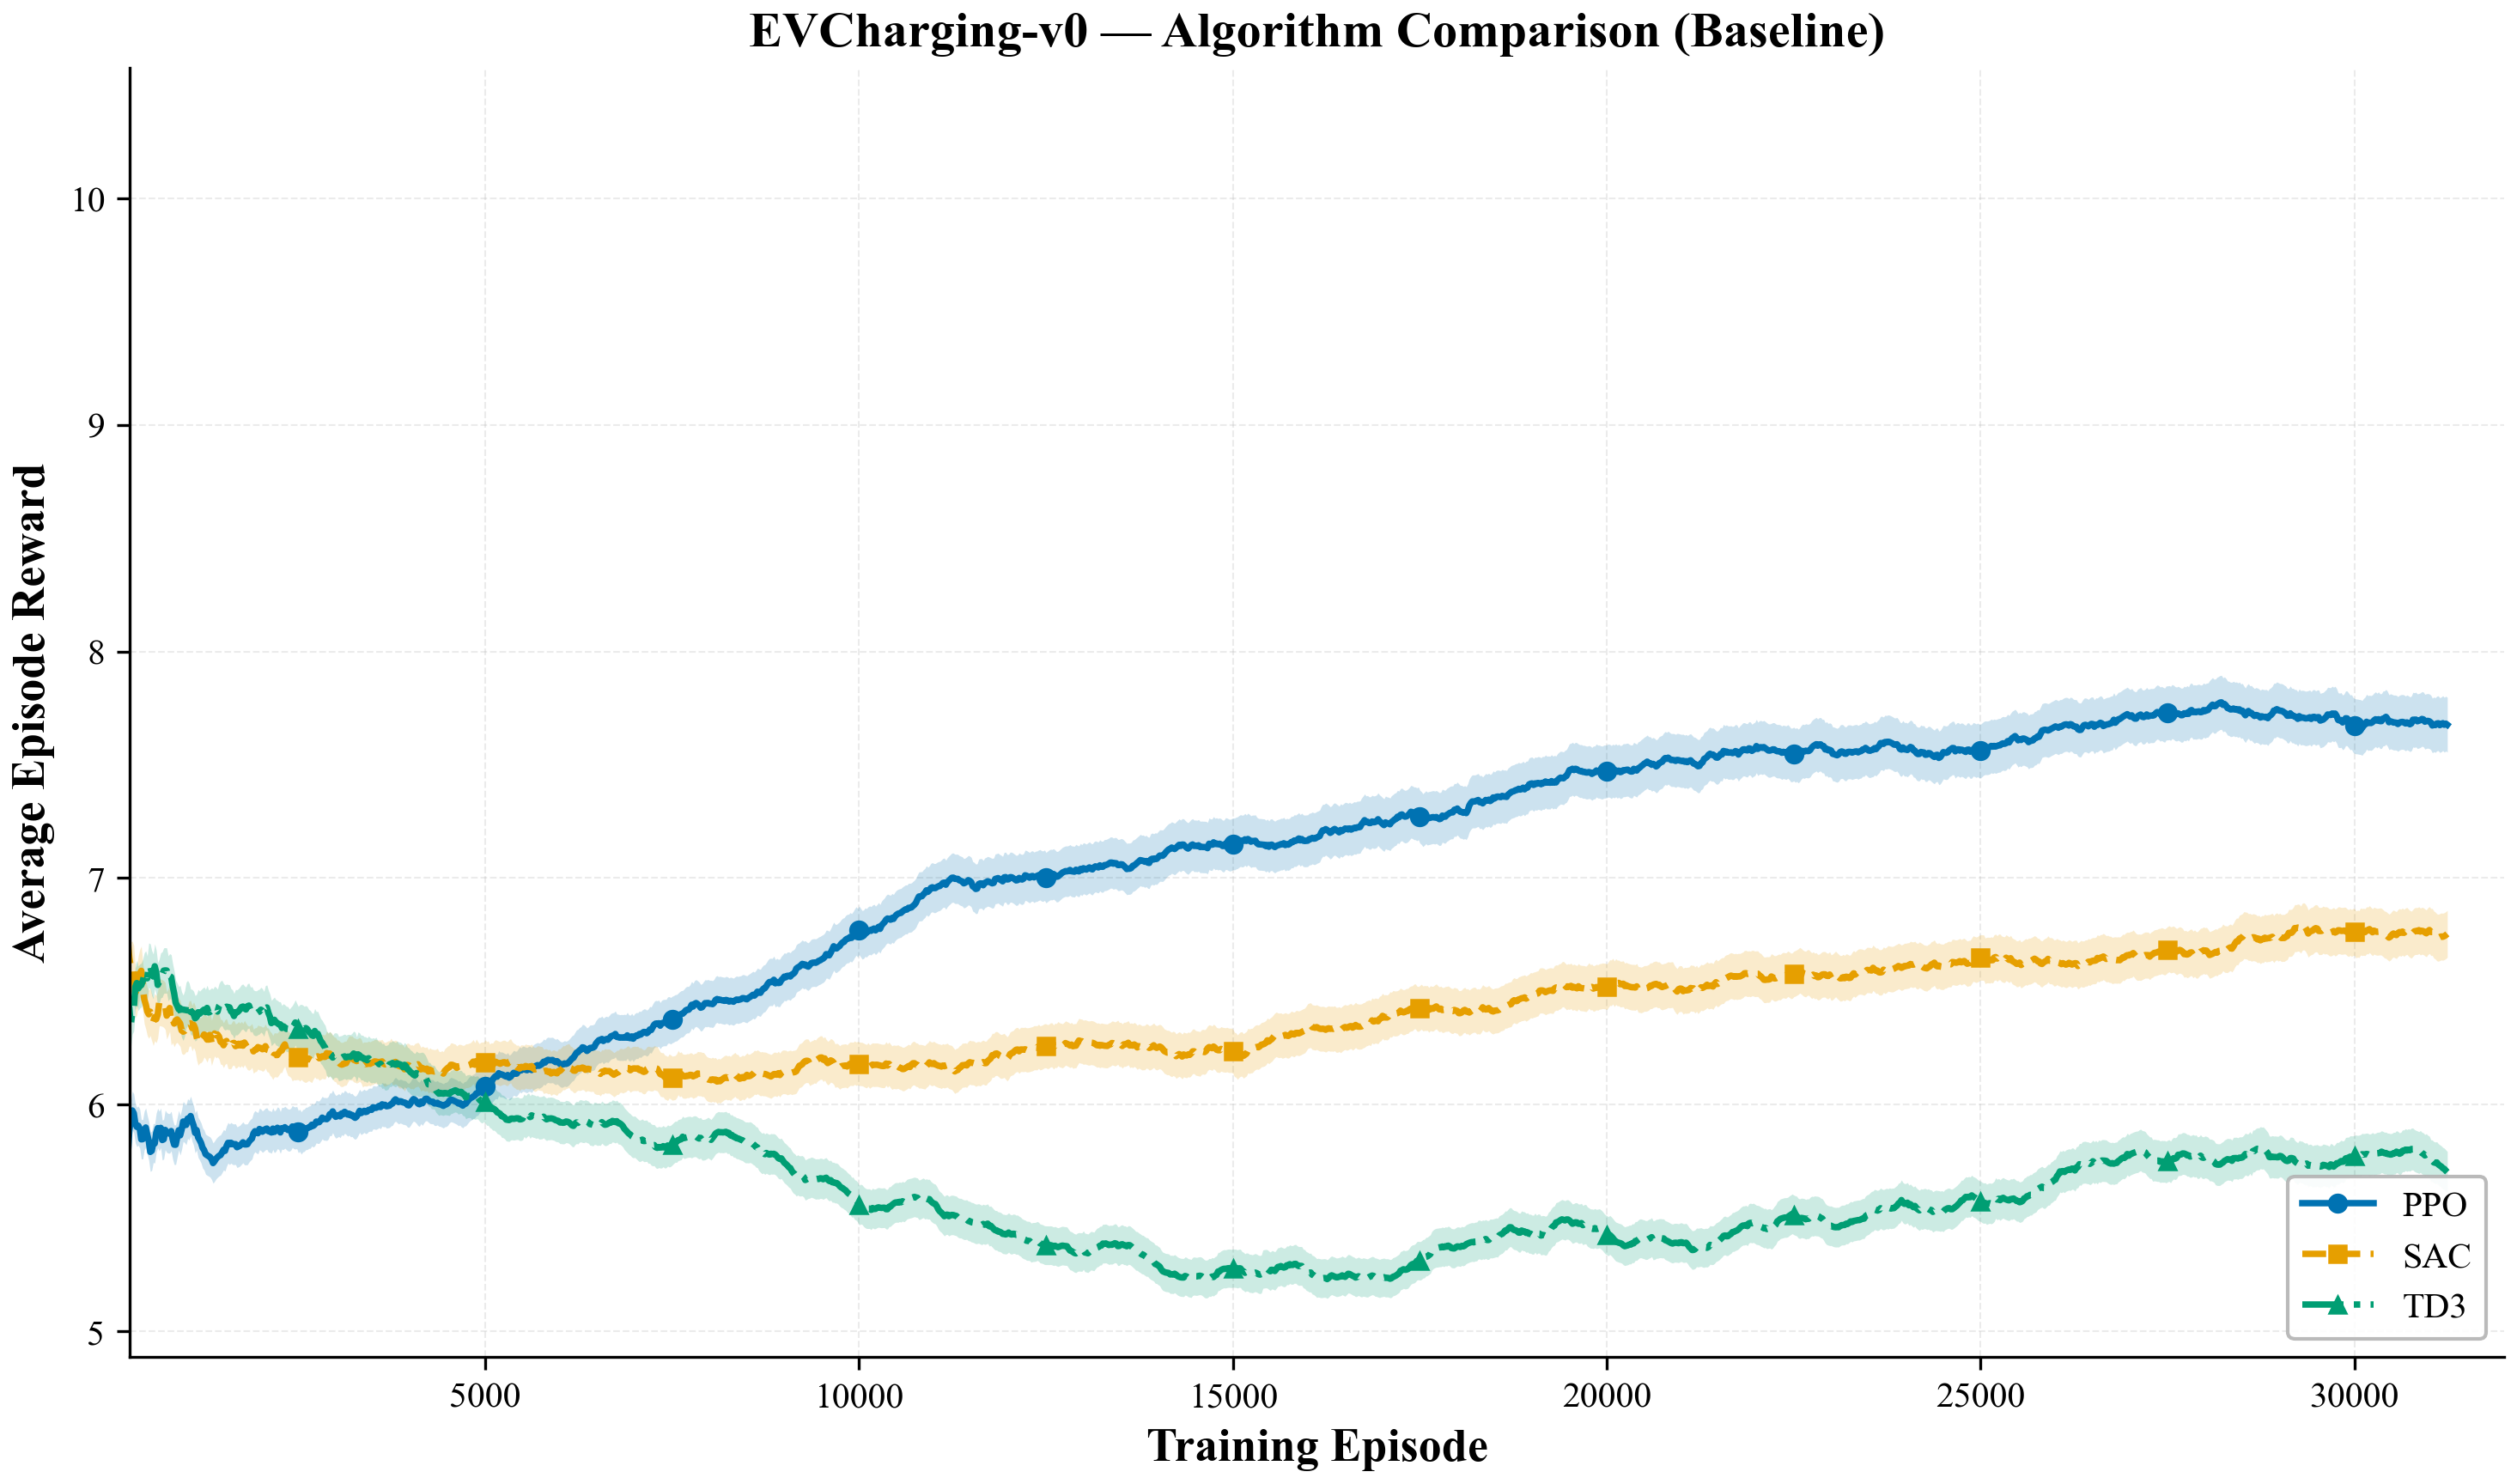
\includegraphics[width=0.9\textwidth]{figures/C_STDRL/ev/comparison/baseline_comparison_2026-03-18_00-03-51.png}
\caption{EV Charging: Baseline training curve comparison across PPO, SAC, and TD3 under clean conditions.}
\label{fig:baseline_ev}
\end{figure}

\begin{figure}[htbp]
\centering
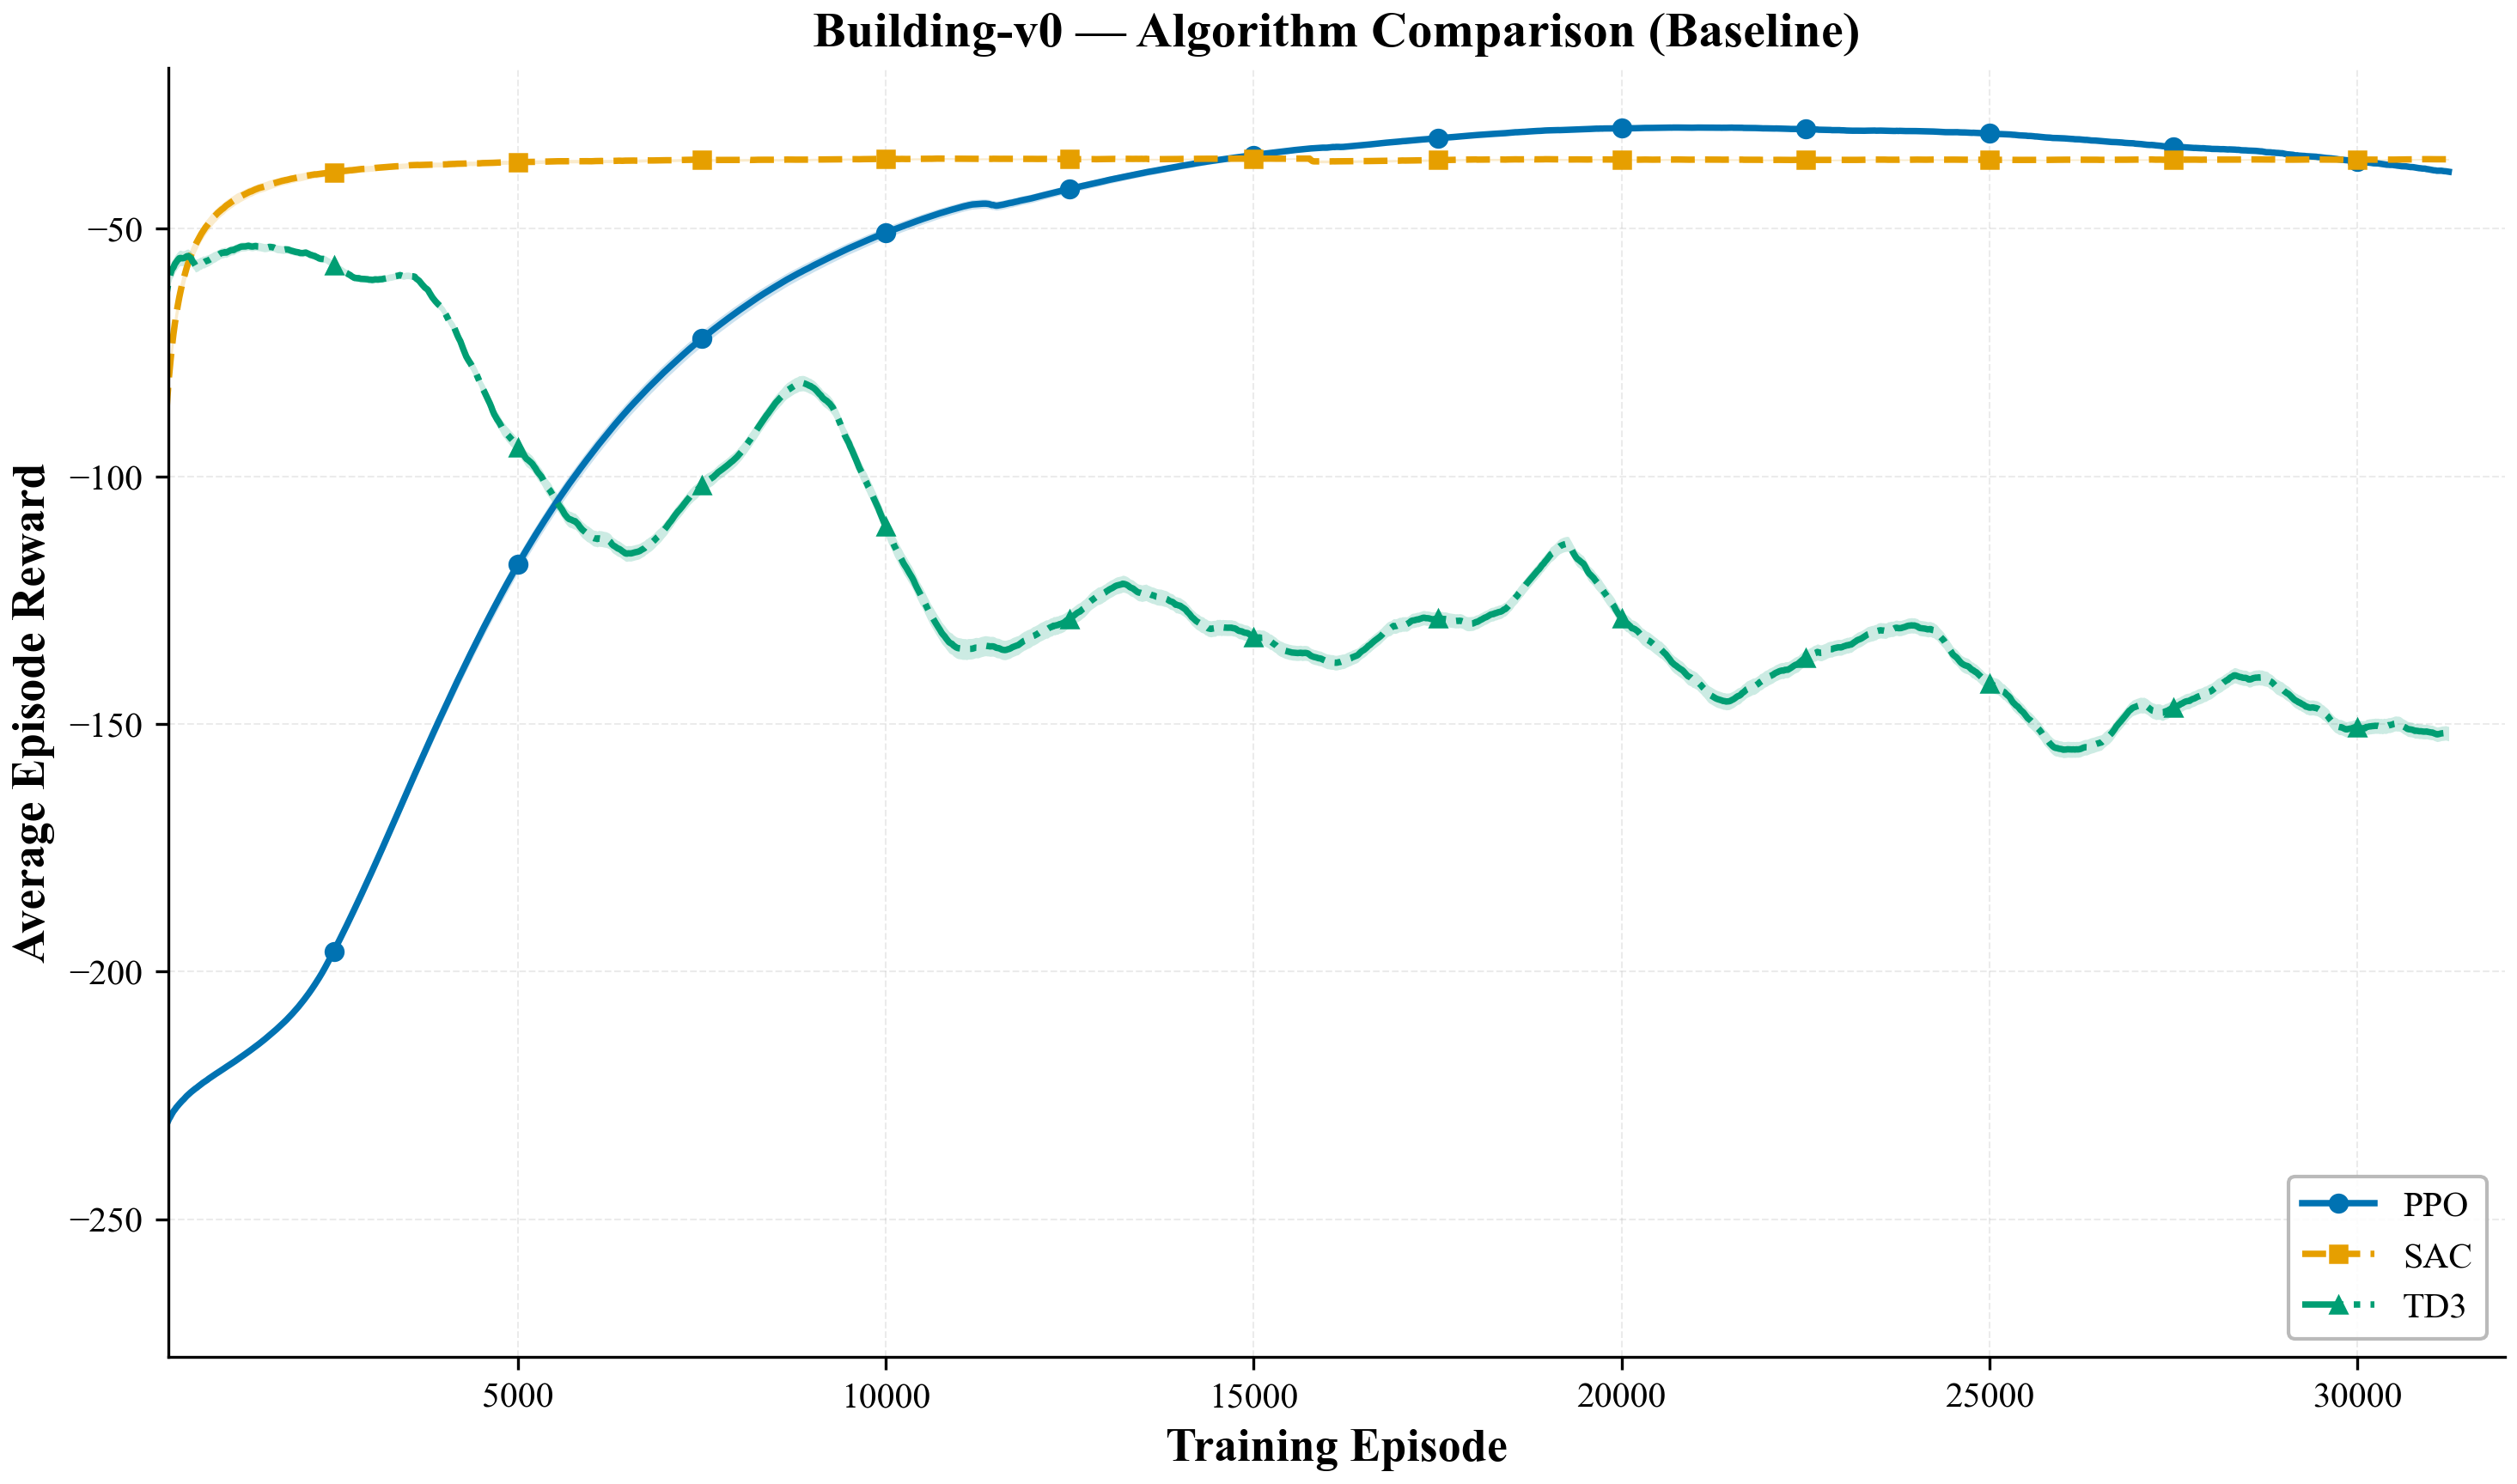
\includegraphics[width=0.9\textwidth]{figures/C_STDRL/bu/comparison/baseline_comparison_2026-03-18_00-04-07.png}
\caption{Building: Baseline training curve comparison across PPO, SAC, and TD3 under clean conditions.}
\label{fig:baseline_bu}
\end{figure}

\begin{figure}[htbp]
\centering
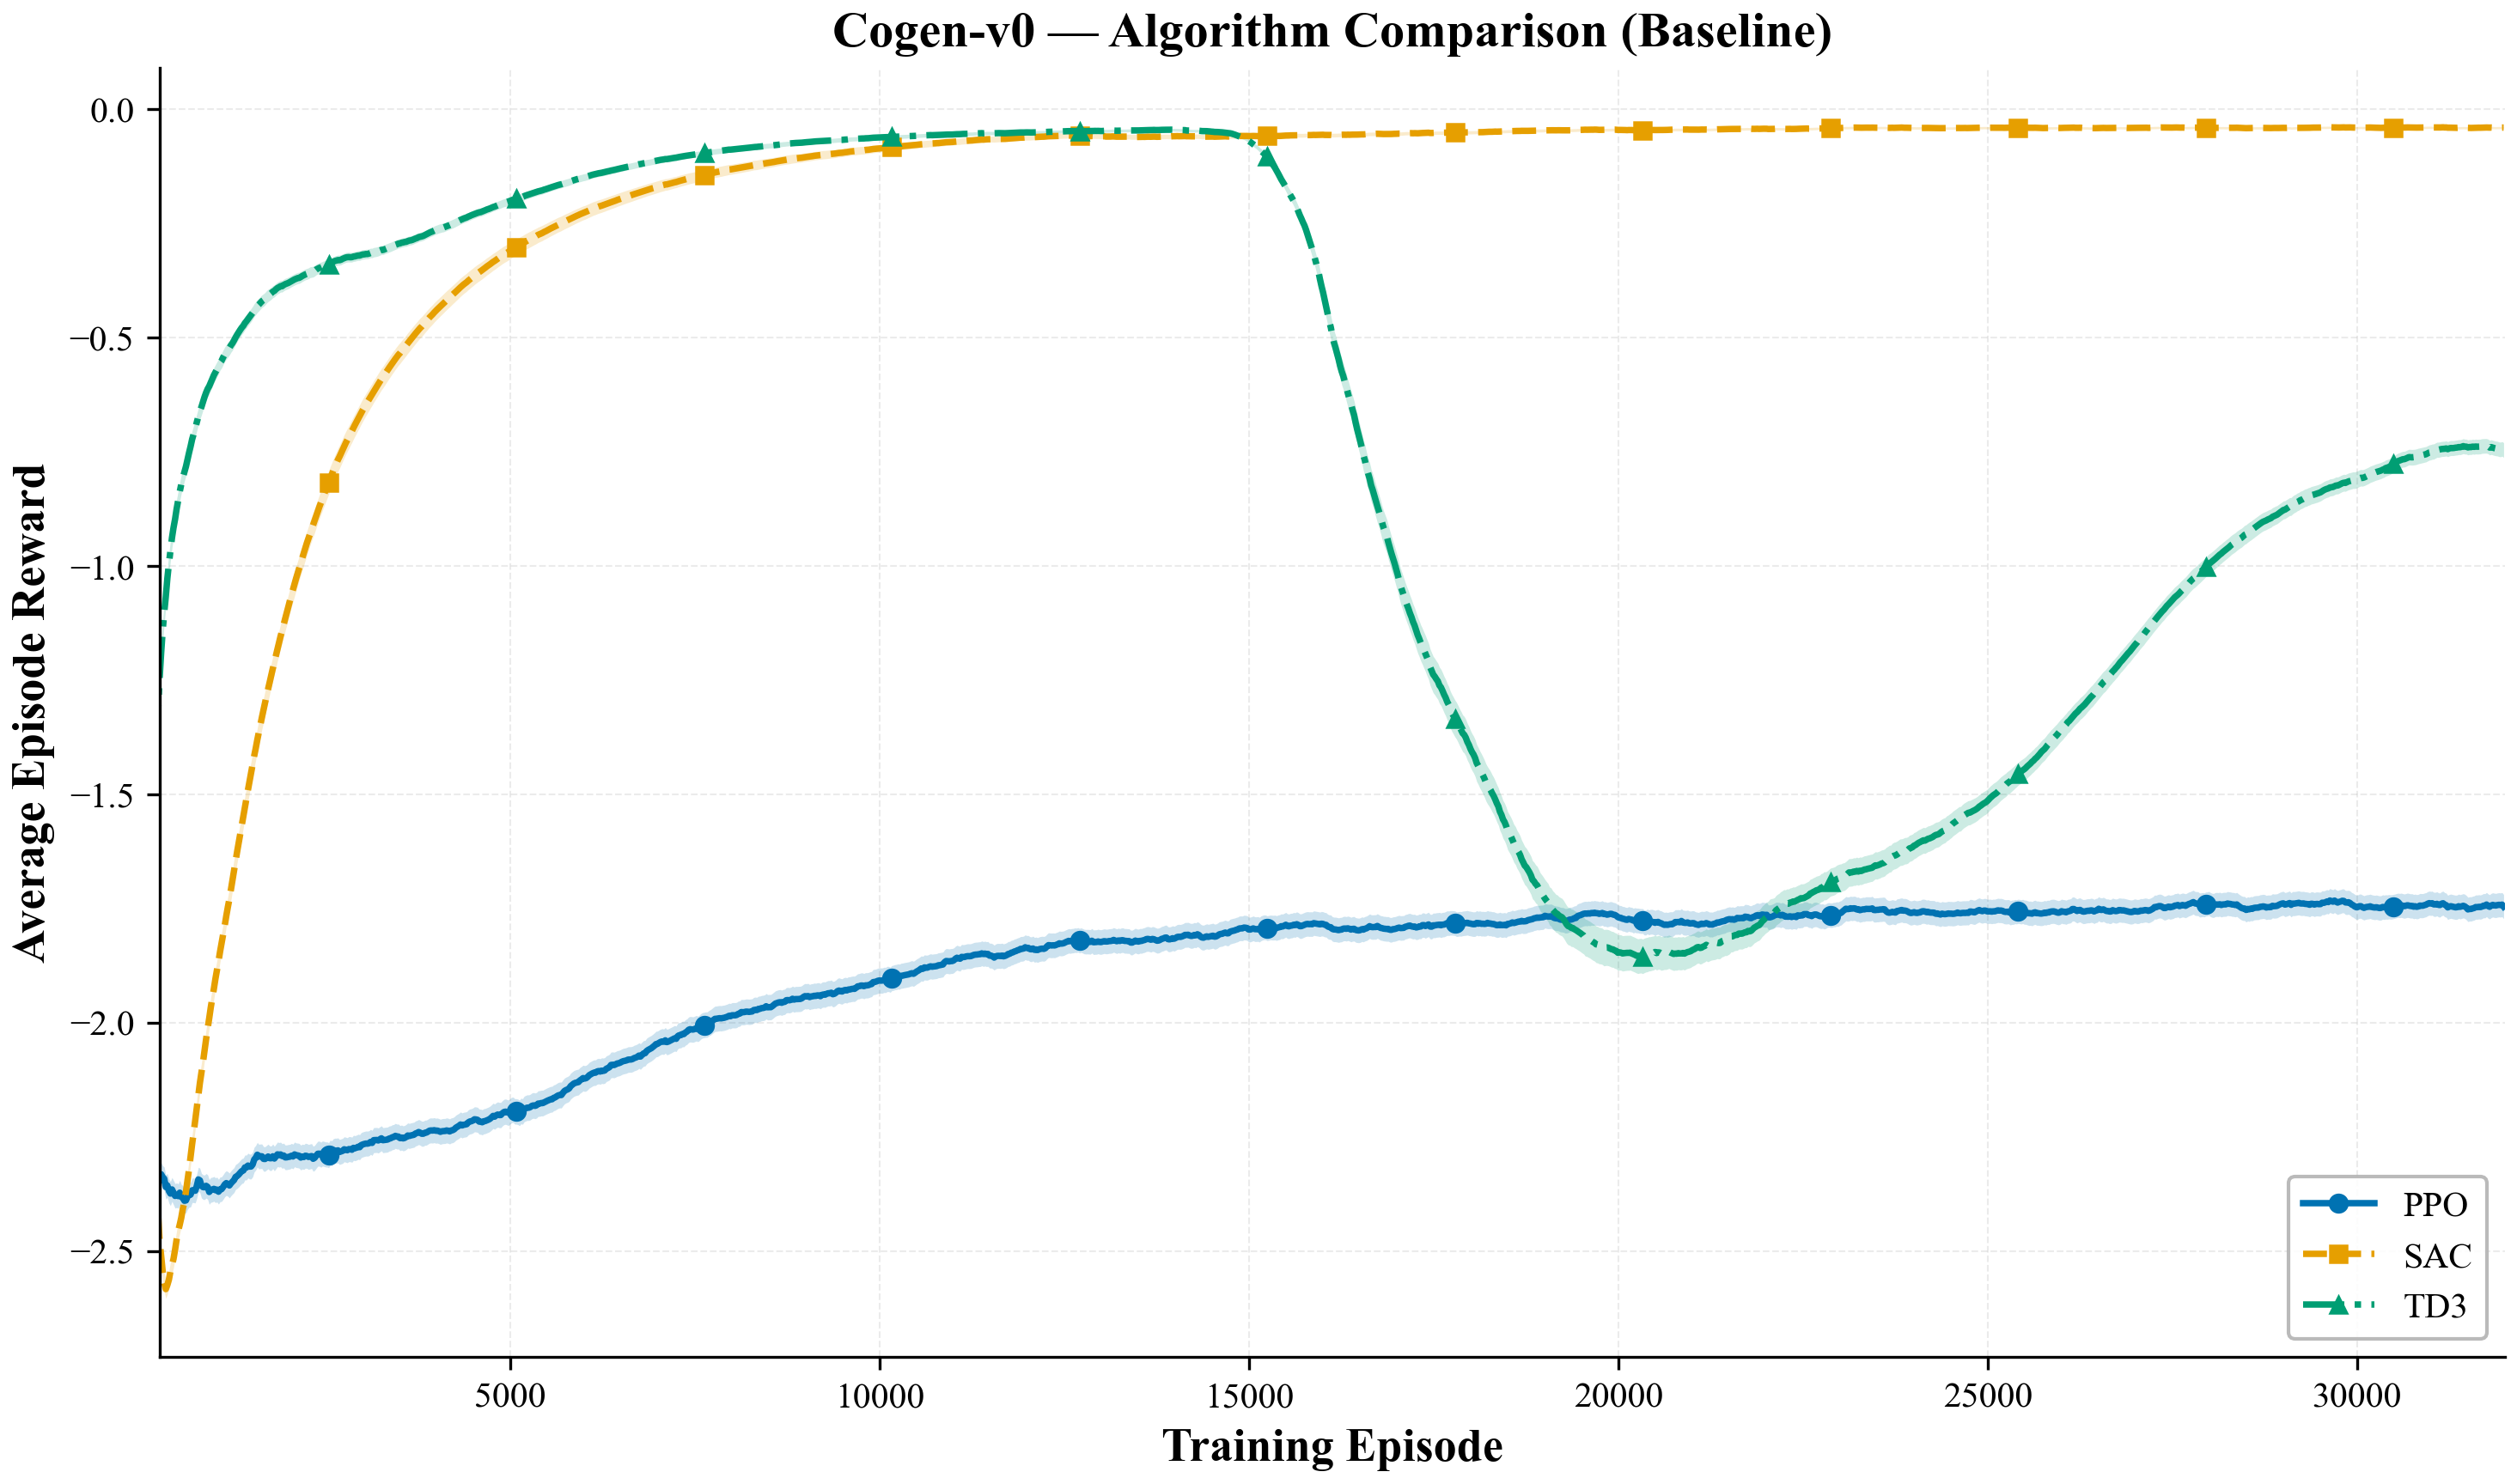
\includegraphics[width=0.9\textwidth]{figures/C_STDRL/co/comparison/baseline_comparison_2026-03-18_00-04-19.png}
\caption{Cogeneration: Baseline training curve comparison across PPO, SAC, and TD3 under clean conditions.}
\label{fig:baseline_co}
\end{figure}

Several environment-specific observations emerge from the baselines:

\paragraph{EV Charging.} PPO significantly outperforms SAC and TD3 in absolute reward ($6.01$ vs.\ $3.79$ and $3.16$), though SAC achieves a slightly higher profit ratio ($0.730$ vs.\ $0.695$). The variance is substantial across all algorithms ($\text{std} \approx 3.1$--$3.5$), reflecting the stochastic nature of EV arrival/departure patterns.

\paragraph{Building.} PPO achieves the best baseline reward ($-32.10$), substantially outperforming TD3 ($-63.20$) and SAC ($-97.71$). The large gap suggests that PPO's on-policy optimization is better suited to the Building environment's multi-zone thermal dynamics. TD3's high variance ($\text{std} = 26.85$) indicates inconsistent HVAC control across episodes.

\paragraph{Cogeneration.} SAC and TD3 achieve near-zero reward ($\approx -0.03$ to $-0.04$), indicating successful plant operation. PPO's reward of $-1.76$ is significantly worse, reflecting PPO's known difficulty with high-dimensional continuous action spaces (15 actuators). However, PPO achieves the lowest fuel cost (\$11,001 vs.\ \$18,700 for SAC), suggesting it learns an overly conservative but fuel-efficient strategy.

% ============================================================
\subsection{EV Charging: Noise Robustness}
\label{sec:noise_ev}

The EV Charging environment exhibits remarkable robustness to all noise types across all algorithms. This resilience stems from the environment's reward structure, which depends primarily on aggregate daily charging patterns rather than instantaneous observations.

% --- EV PPO ---
\subsubsection{EV Charging --- PPO}

\paragraph{Training curves.} \Cref{fig:stdrl_ev_ppo_ds,fig:stdrl_ev_ppo_da,fig:stdrl_ev_ppo_de} show PPO training curves under observation, action, and environment noise respectively. Convergence is virtually unaffected across all noise levels, with final rewards clustering tightly around the clean baseline.

\begin{figure}[htbp]
\centering
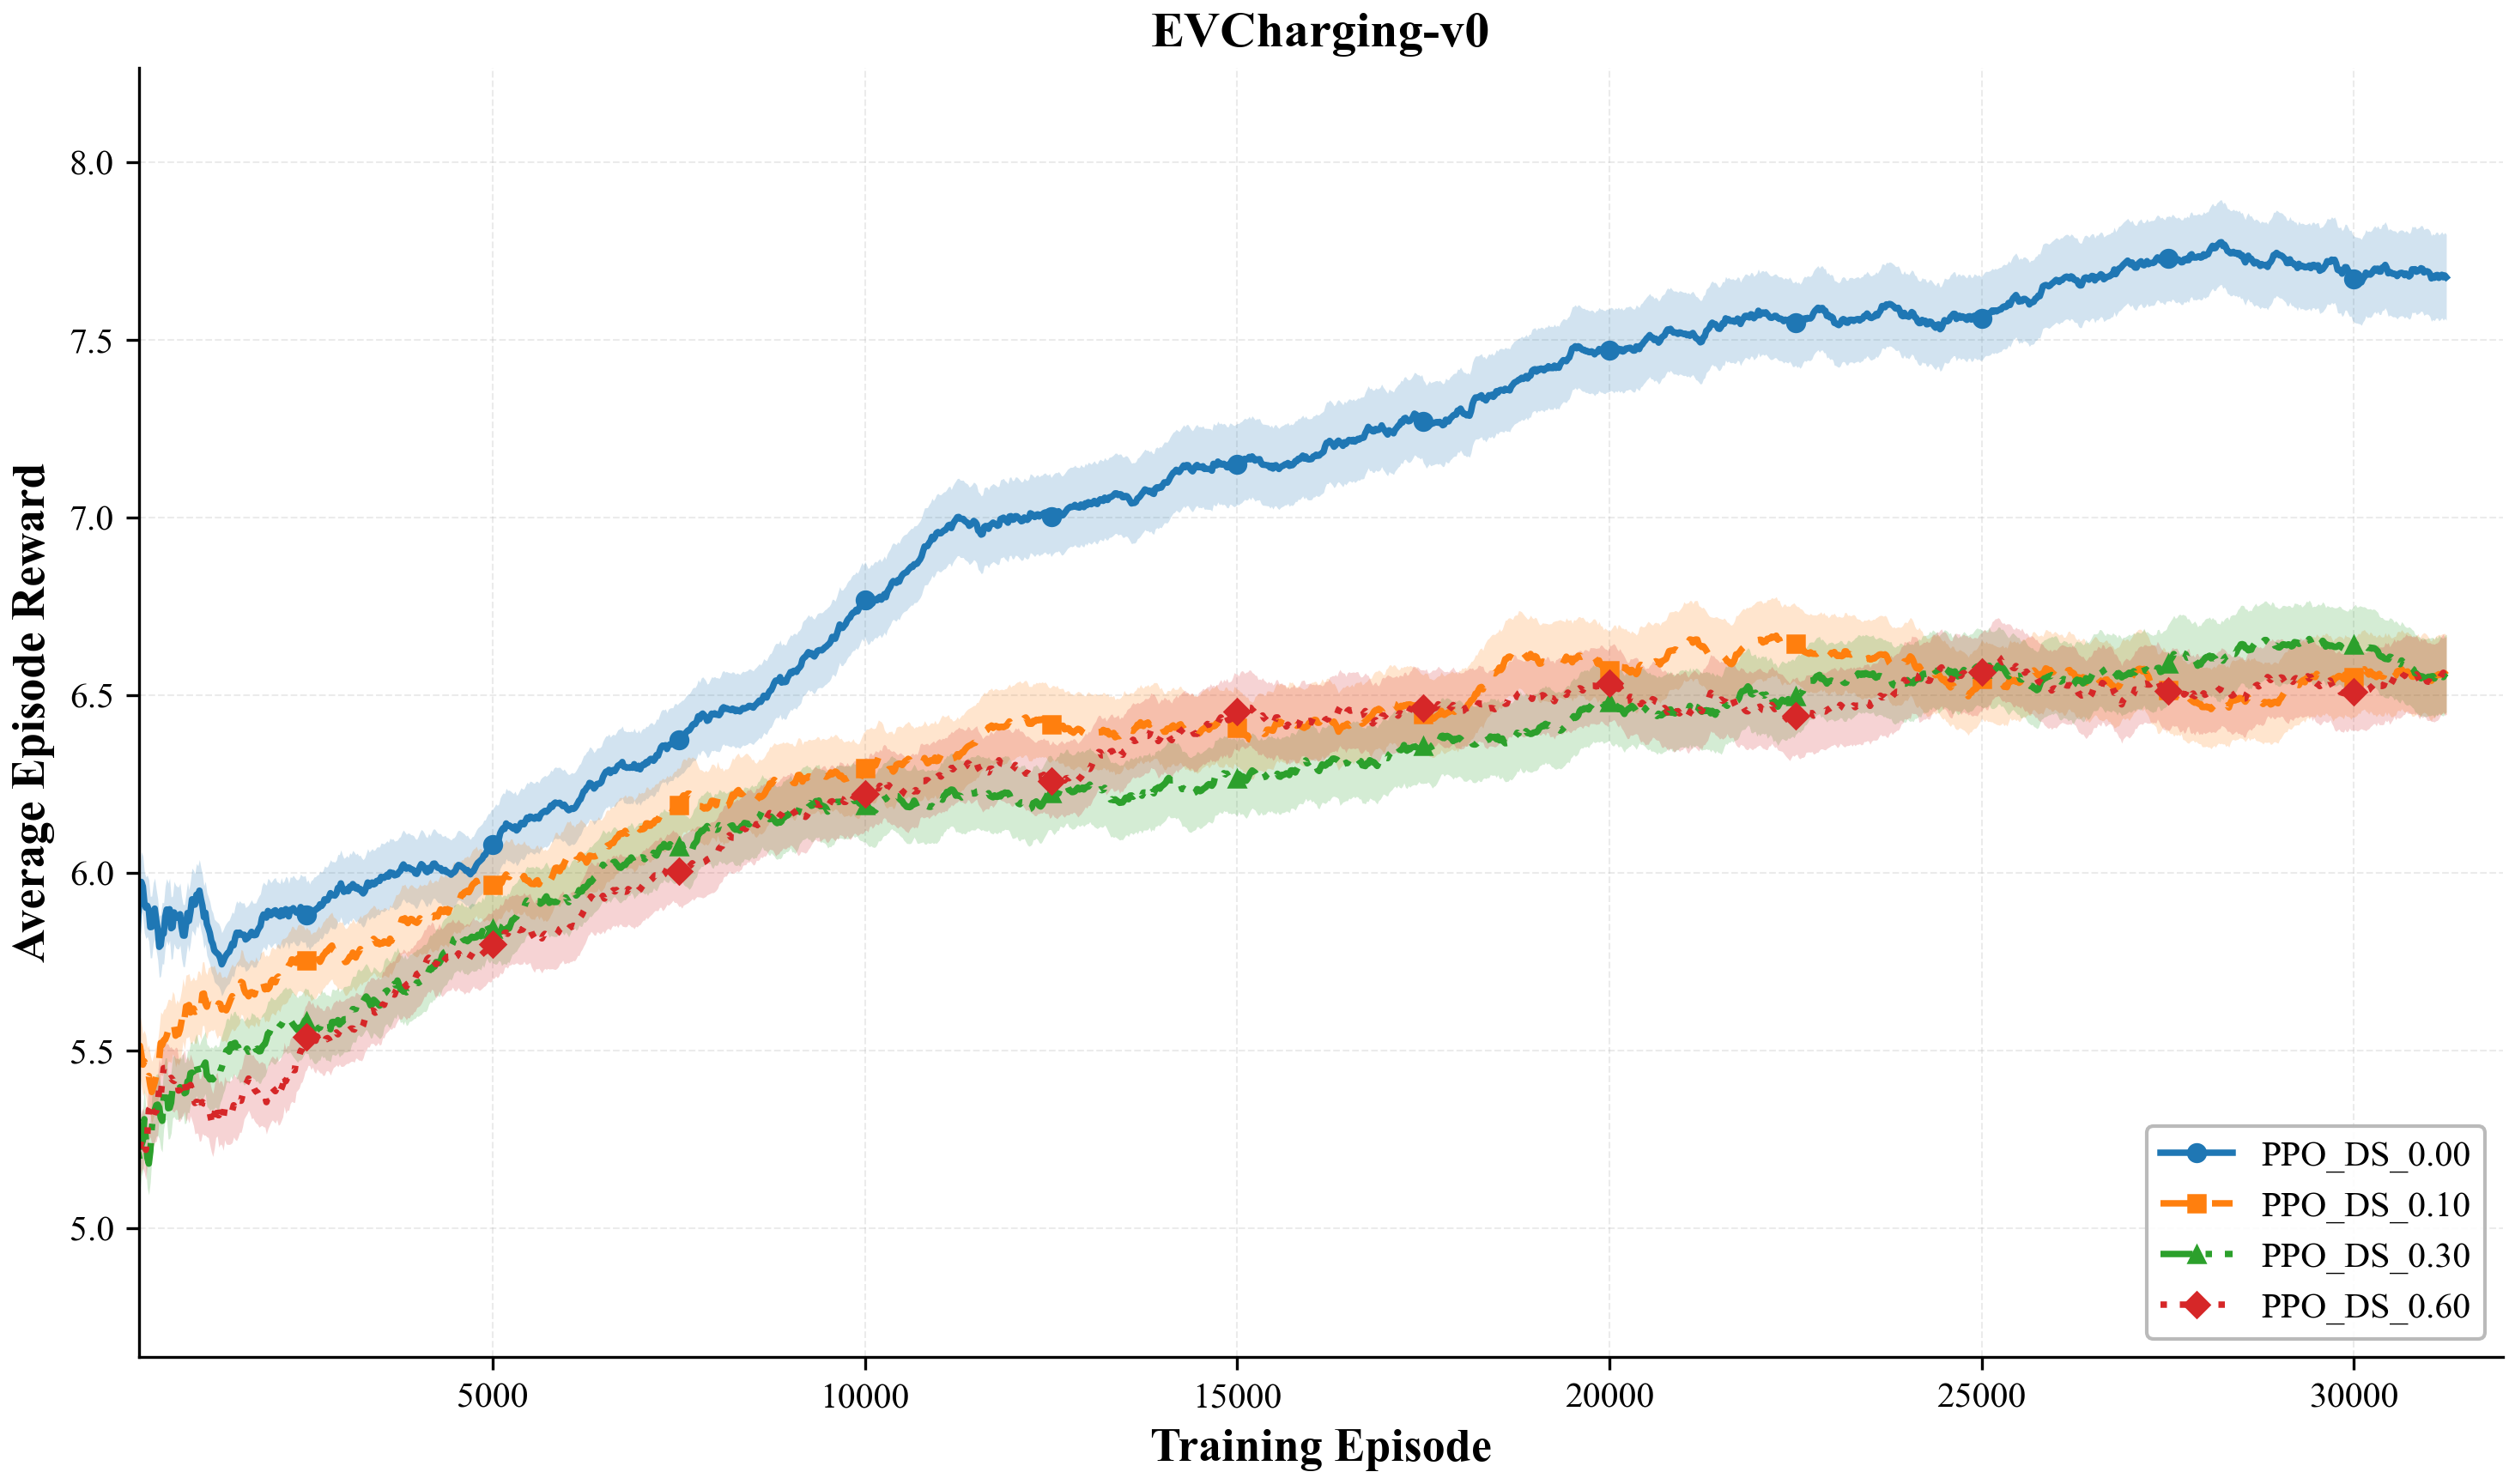
\includegraphics[width=0.9\textwidth]{figures/C_STDRL/ev/PPO/DS_2026-03-16_23-32-01.png}
\caption{EV Charging PPO: Training curves under observation noise (DS) at varying intensities.}
\label{fig:stdrl_ev_ppo_ds}
\end{figure}

\begin{figure}[htbp]
\centering
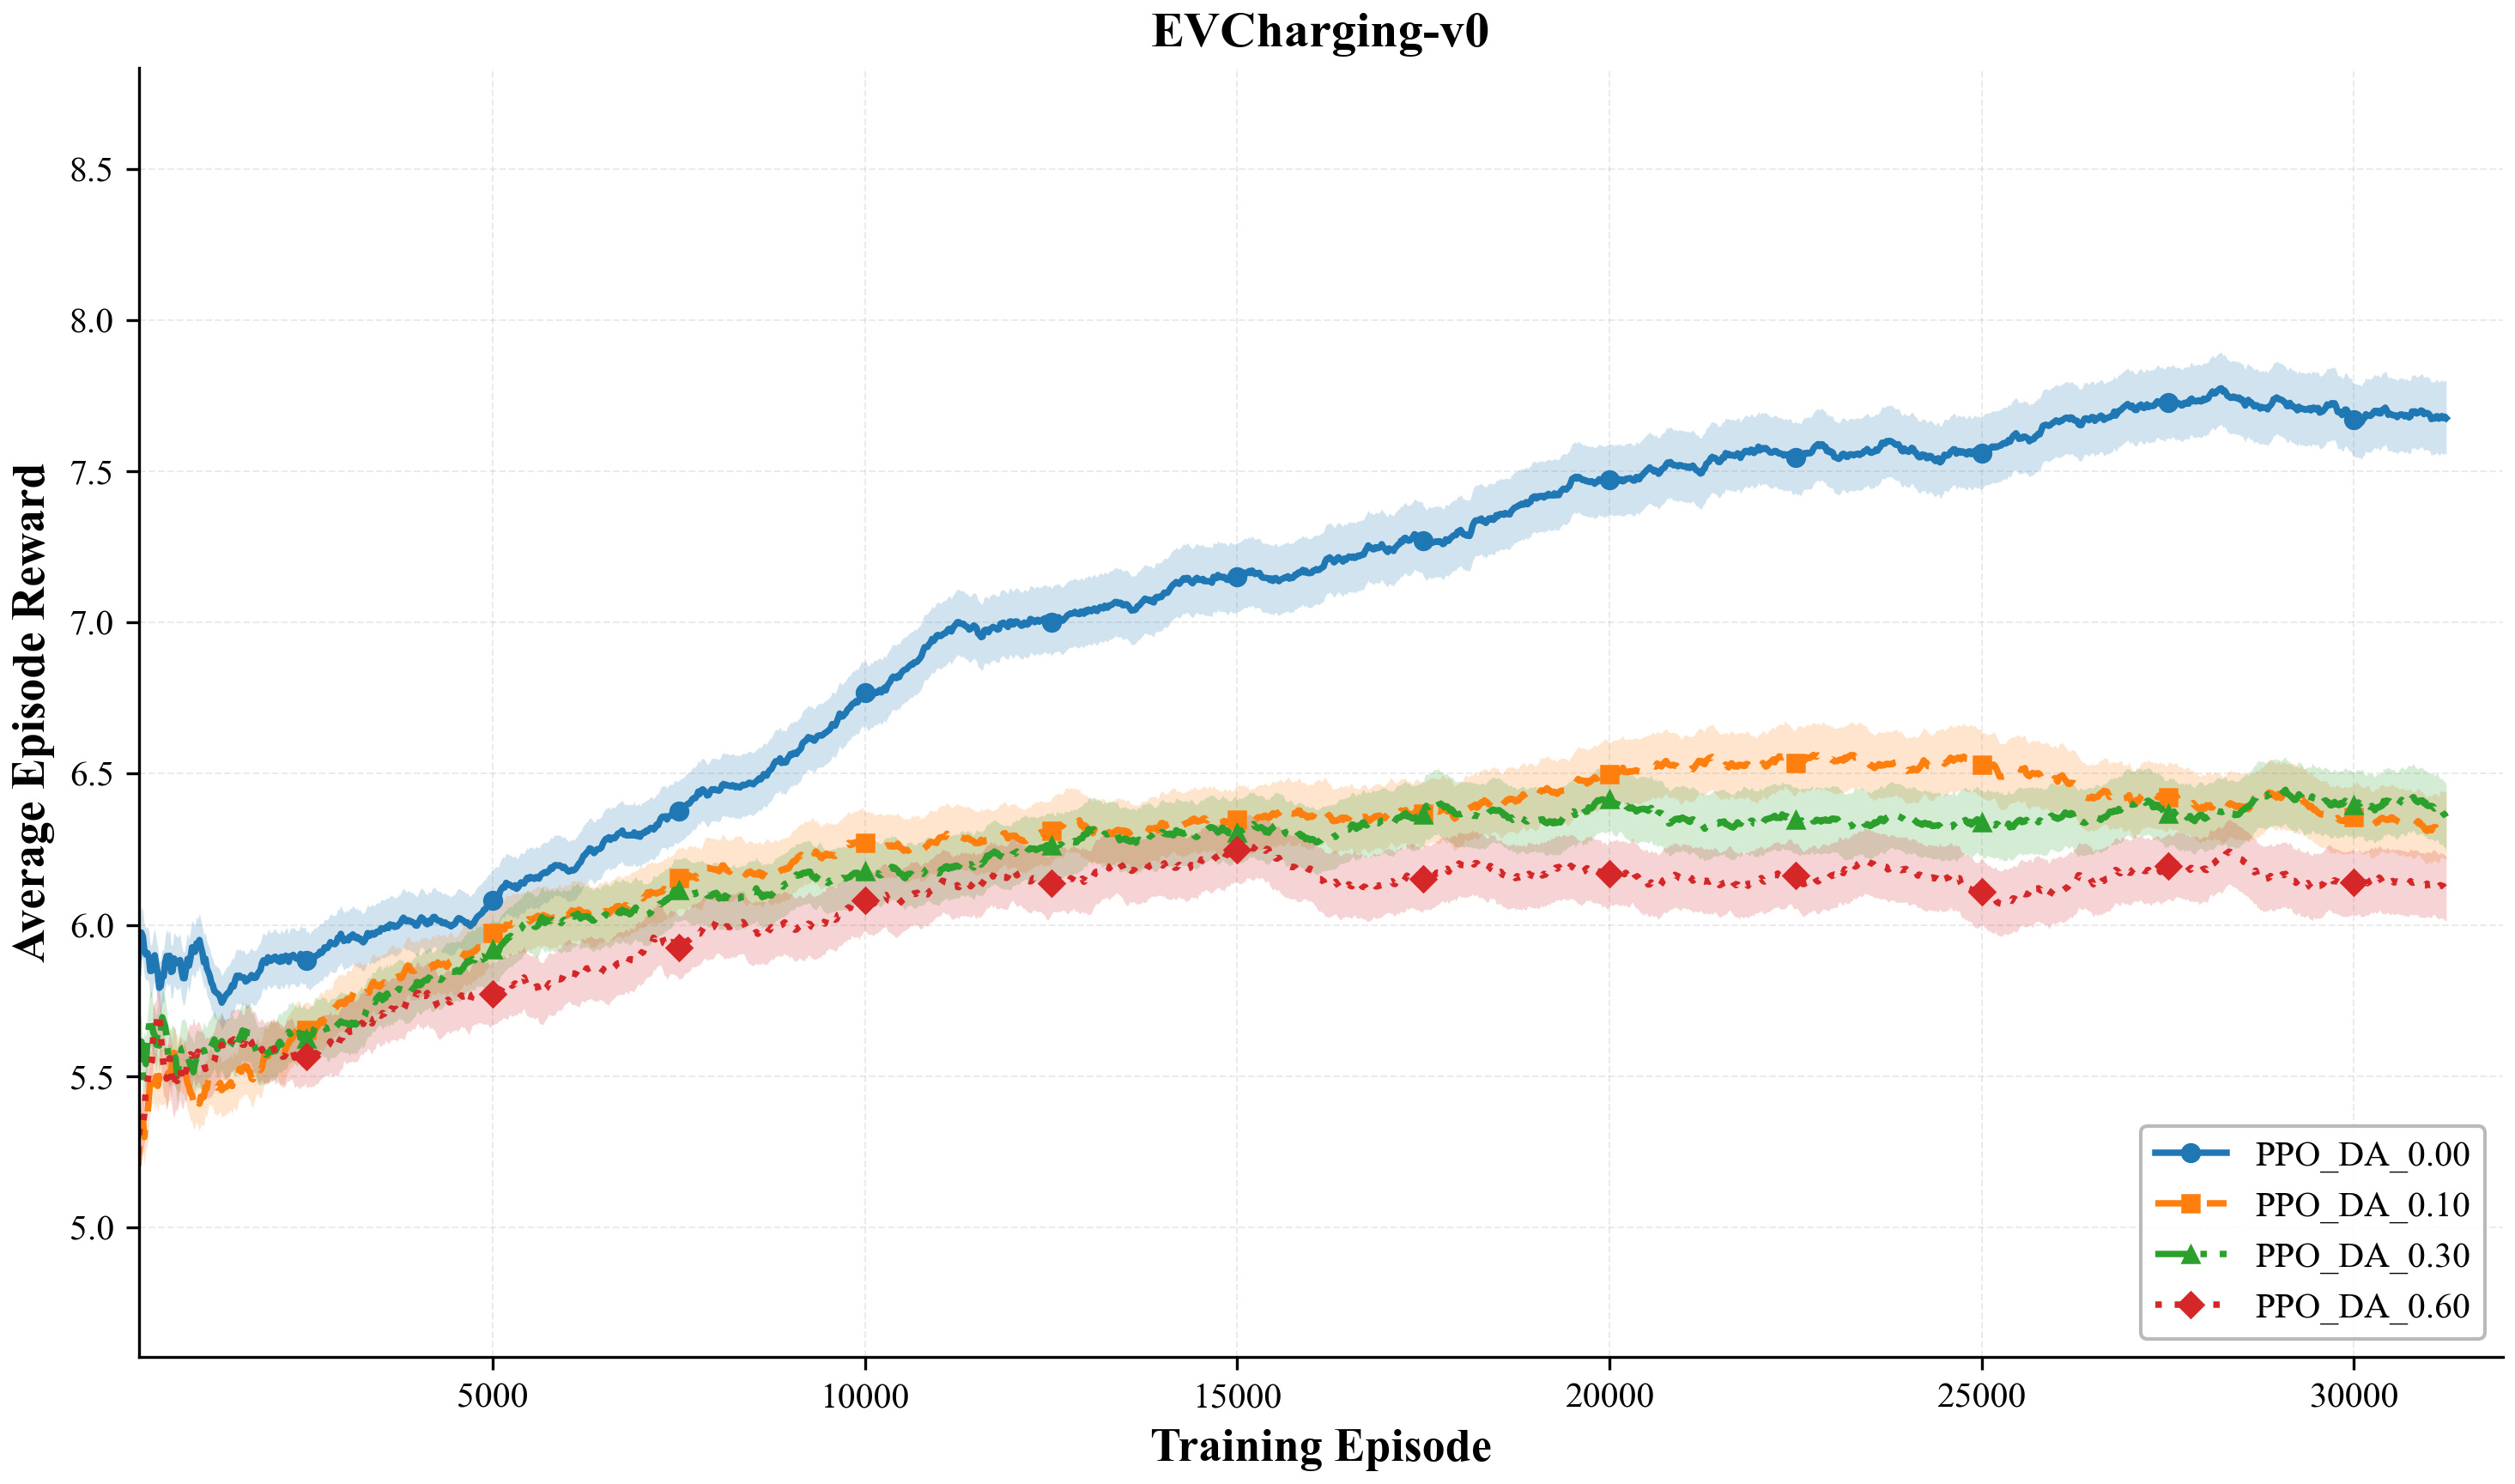
\includegraphics[width=0.9\textwidth]{figures/C_STDRL/ev/PPO/DA_2026-03-16_23-32-03.png}
\caption{EV Charging PPO: Training curves under action noise (DA) at varying intensities.}
\label{fig:stdrl_ev_ppo_da}
\end{figure}

\begin{figure}[htbp]
\centering
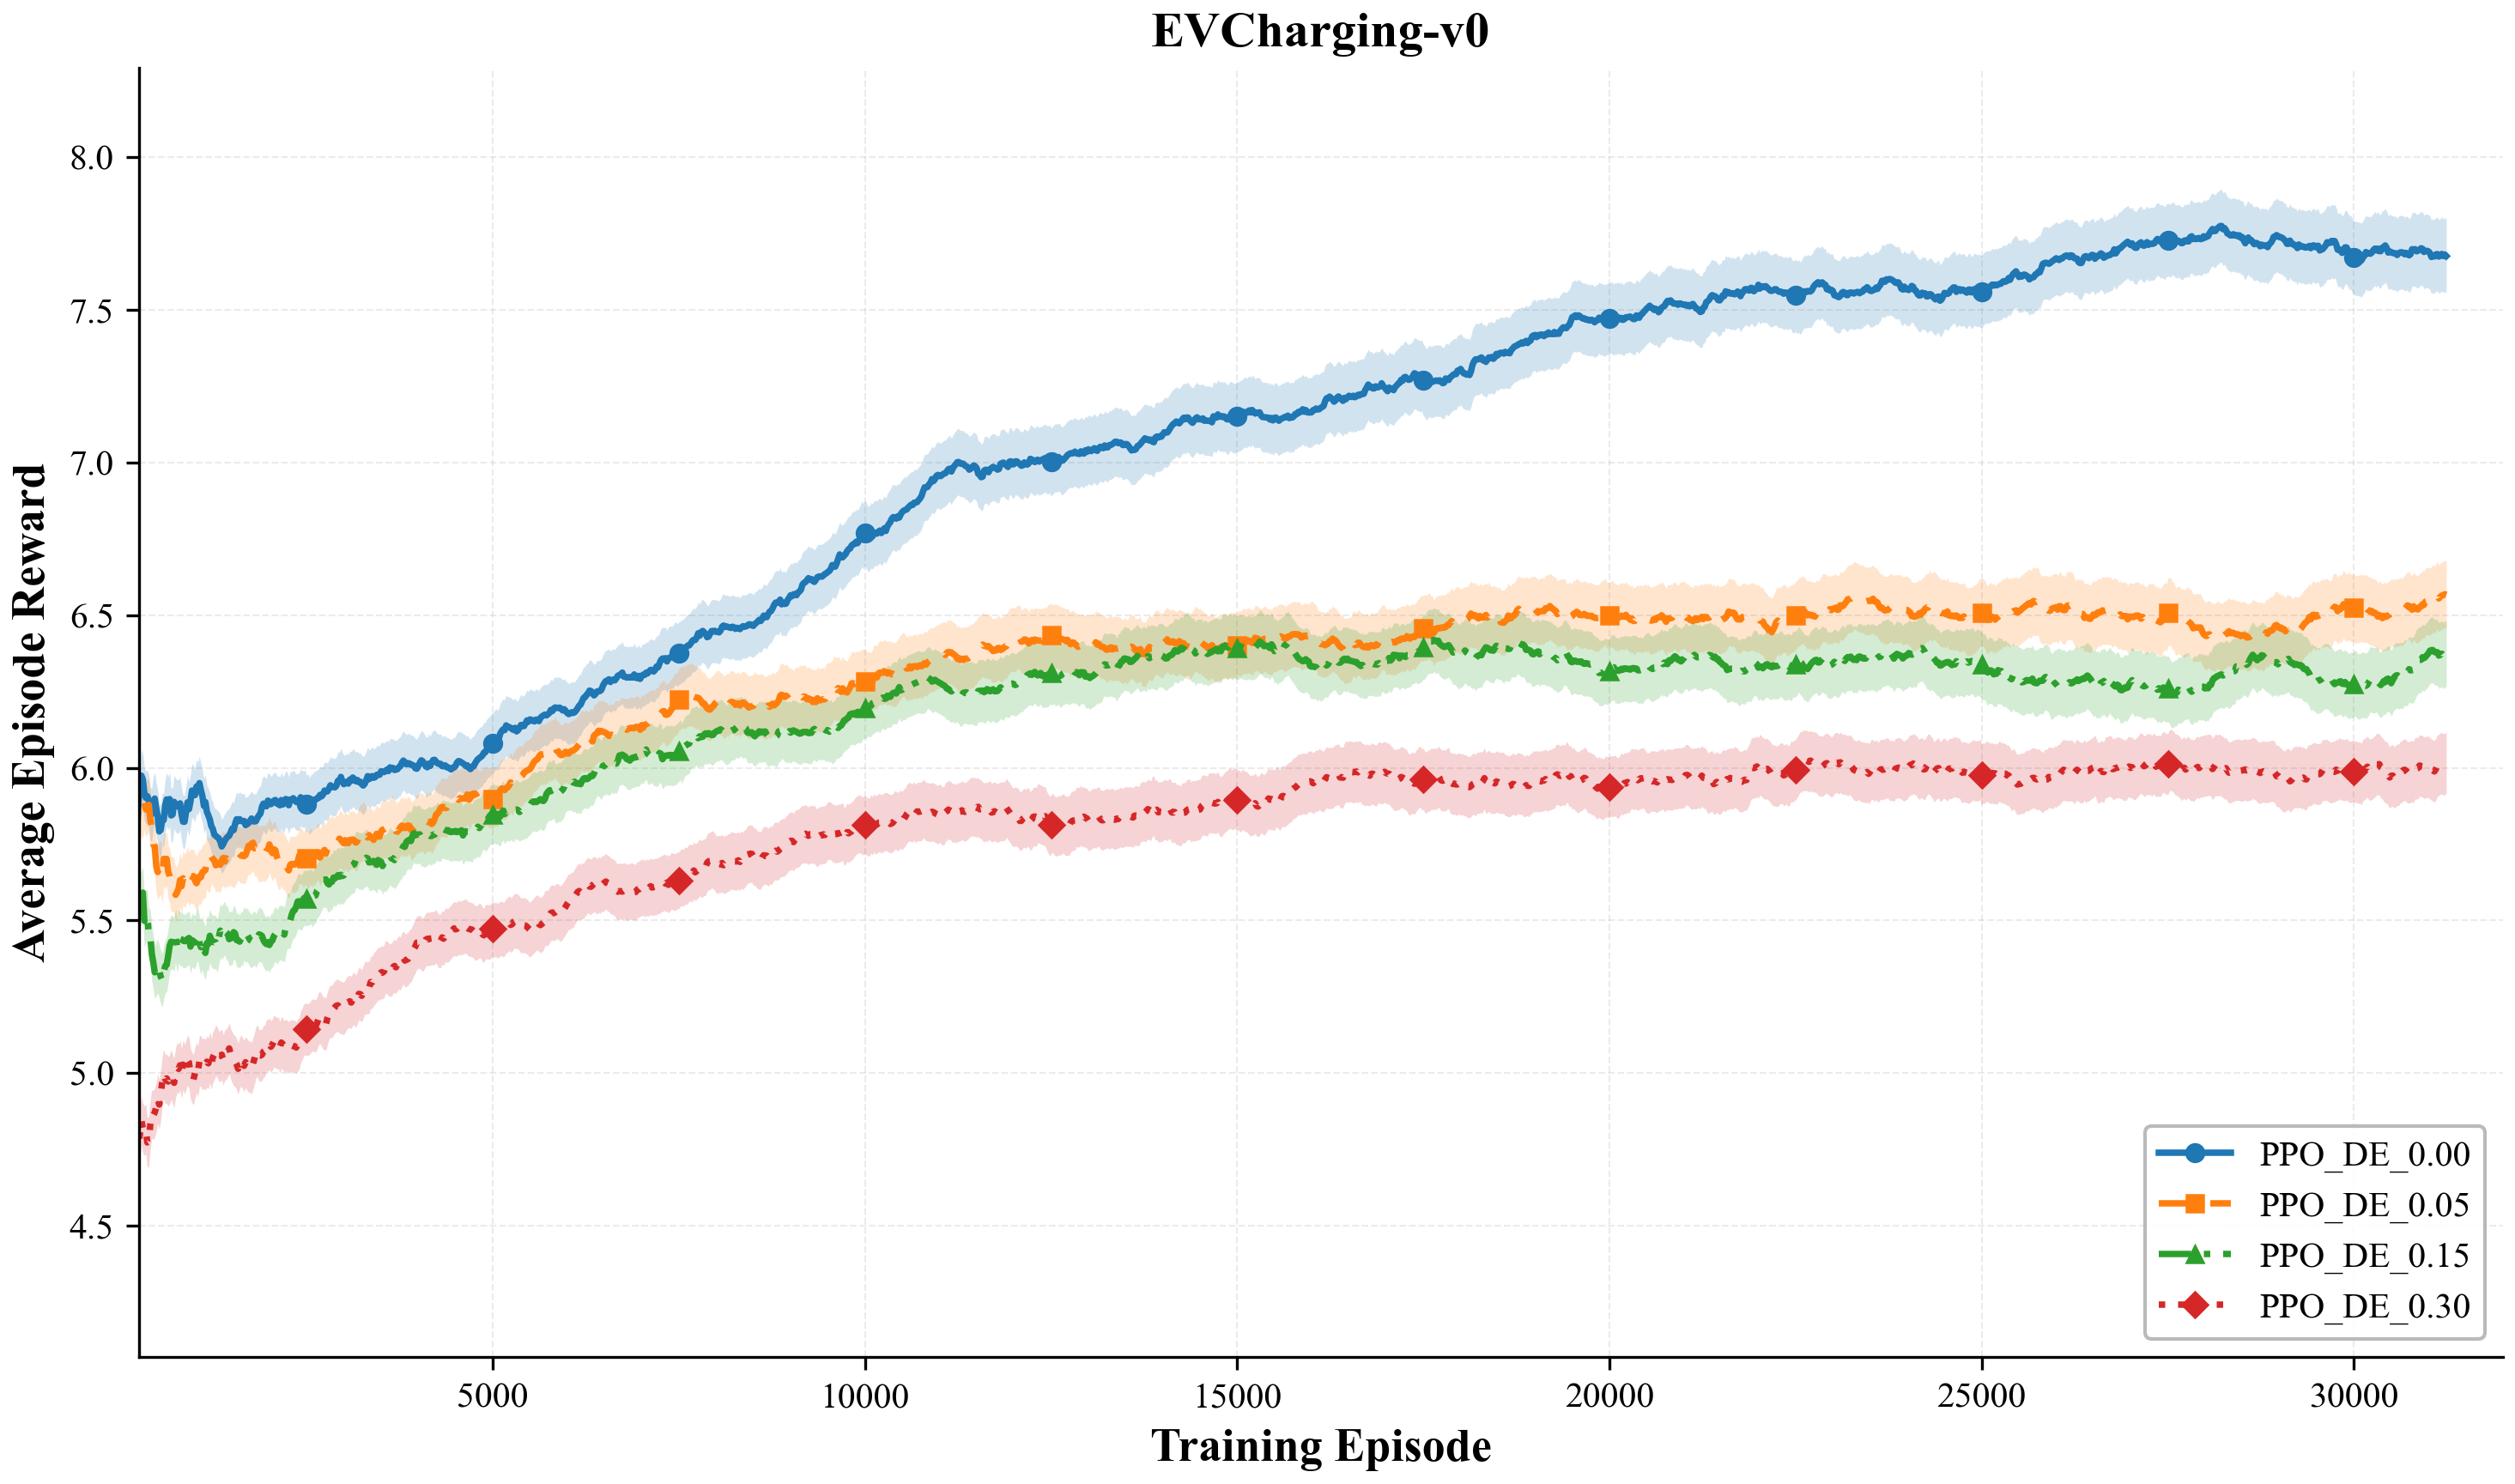
\includegraphics[width=0.9\textwidth]{figures/C_STDRL/ev/PPO/DE_2026-03-16_23-32-04.png}
\caption{EV Charging PPO: Training curves under environment noise (DE) at varying intensities.}
\label{fig:stdrl_ev_ppo_de}
\end{figure}

\paragraph{Test-time robustness.} The violin plots in \Cref{fig:violin_ev_ppo_obs,fig:violin_ev_ppo_act,fig:violin_ev_ppo_env} confirm that the reward distribution remains stable across all noise channels. The distributional shape is virtually unchanged even at extreme noise levels, with no shift in the mode or emergence of heavy tails.

\begin{figure}[htbp]
\centering

\includegraphics[width=0.9\textwidth]{figures/C_POST/evcharging/PPO/obs_violin.png}
\caption{EV Charging PPO: Reward distribution under observation noise. The distribution remains stable across noise levels, confirming exceptional robustness to sensor uncertainty.}
\label{fig:violin_ev_ppo_obs}
\end{figure}

\begin{figure}[htbp]
\centering

\includegraphics[width=0.9\textwidth]{figures/C_POST/evcharging/PPO/action_violin.png}
\caption{EV Charging PPO: Reward distribution under action noise.}
\label{fig:violin_ev_ppo_act}
\end{figure}

\begin{figure}[htbp]
\centering

\includegraphics[width=0.9\textwidth]{figures/C_POST/evcharging/PPO/env_violin.png}
\caption{EV Charging PPO: Reward distribution under environment noise.}
\label{fig:violin_ev_ppo_env}
\end{figure}

\begin{figure}[htbp]
\centering

\includegraphics[width=0.9\textwidth]{figures/C_POST/evcharging/PPO/panel.png}
\caption{EV Charging PPO: Summary panel across all three noise channels. Mean reward degradation is negligible ($<1\%$) across the full noise range.}
\label{fig:post_ev_ppo_panel}
\end{figure}

% --- EV SAC ---
\subsubsection{EV Charging --- SAC}

\paragraph{Training curves.} \Cref{fig:stdrl_ev_sac_ds,fig:stdrl_ev_sac_da,fig:stdrl_ev_sac_de} show SAC training curves under all noise types.

\begin{figure}[htbp]
\centering
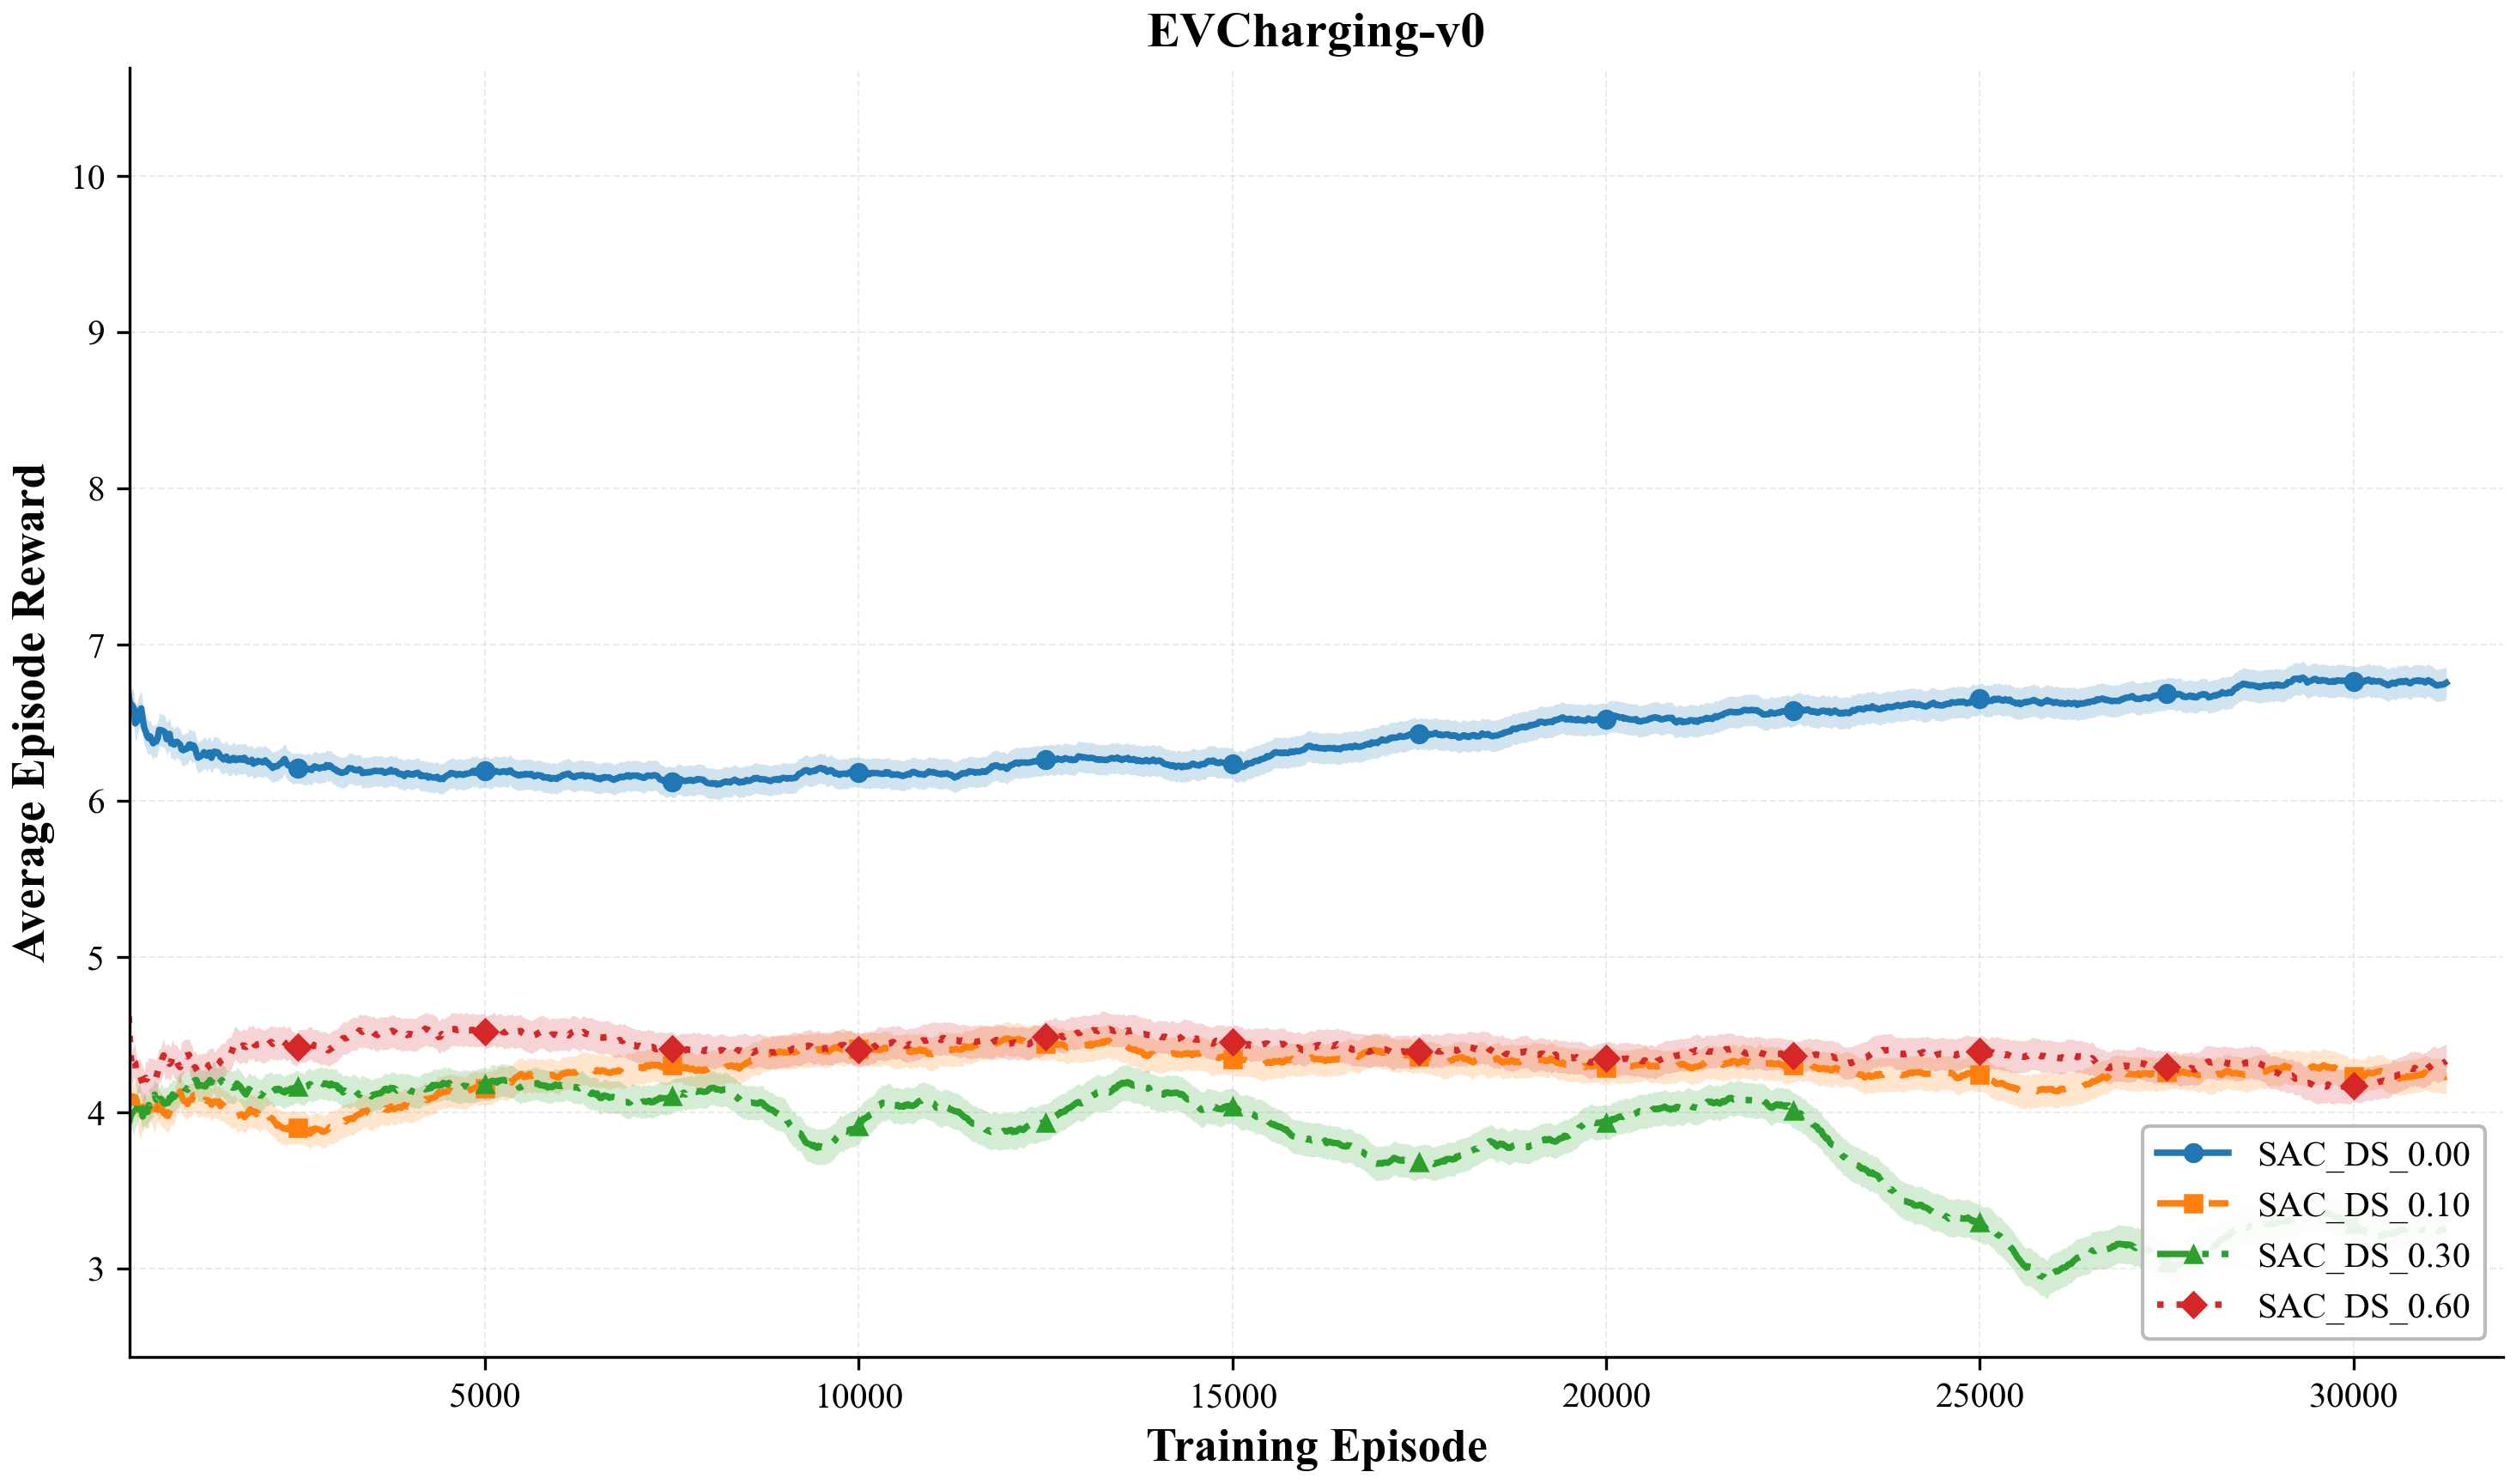
\includegraphics[width=0.9\textwidth]{figures/C_STDRL/ev/SAC/DS_2026-03-16_23-32-06.png}
\caption{EV Charging SAC: Training curves under observation noise (DS).}
\label{fig:stdrl_ev_sac_ds}
\end{figure}

\begin{figure}[htbp]
\centering
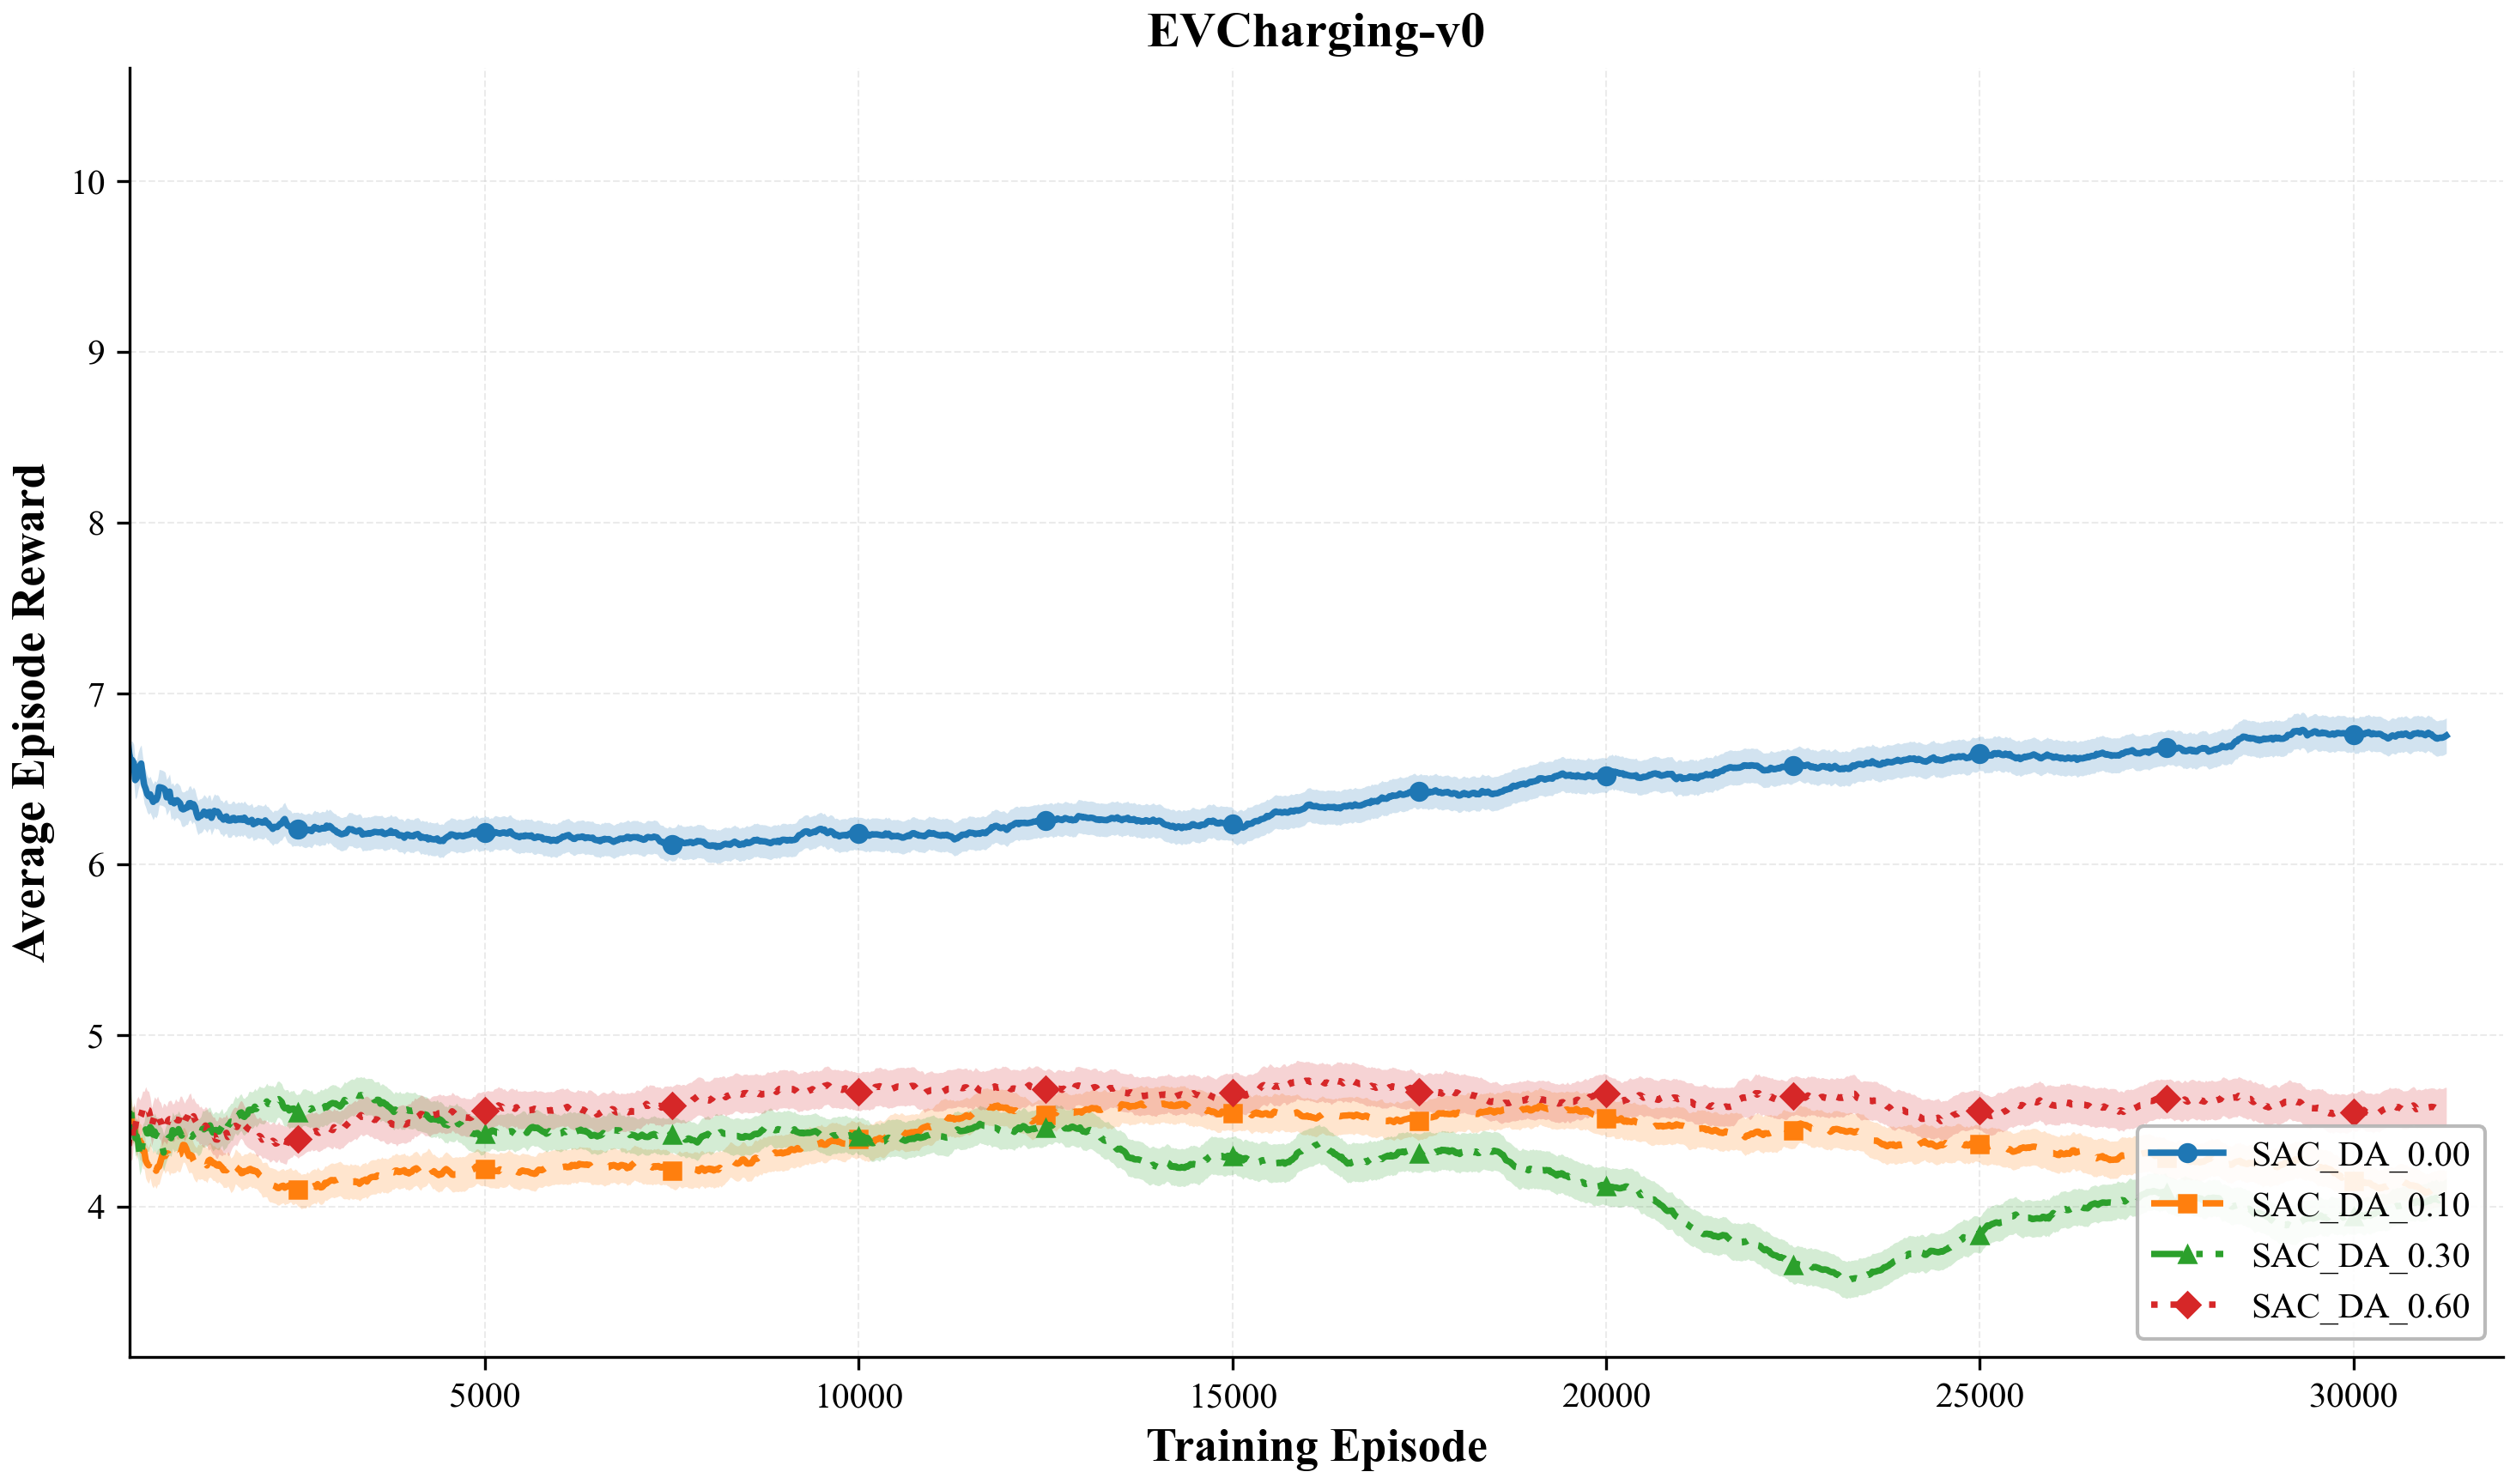
\includegraphics[width=0.9\textwidth]{figures/C_STDRL/ev/SAC/DA_2026-03-16_23-32-09.png}
\caption{EV Charging SAC: Training curves under action noise (DA).}
\label{fig:stdrl_ev_sac_da}
\end{figure}

\begin{figure}[htbp]
\centering
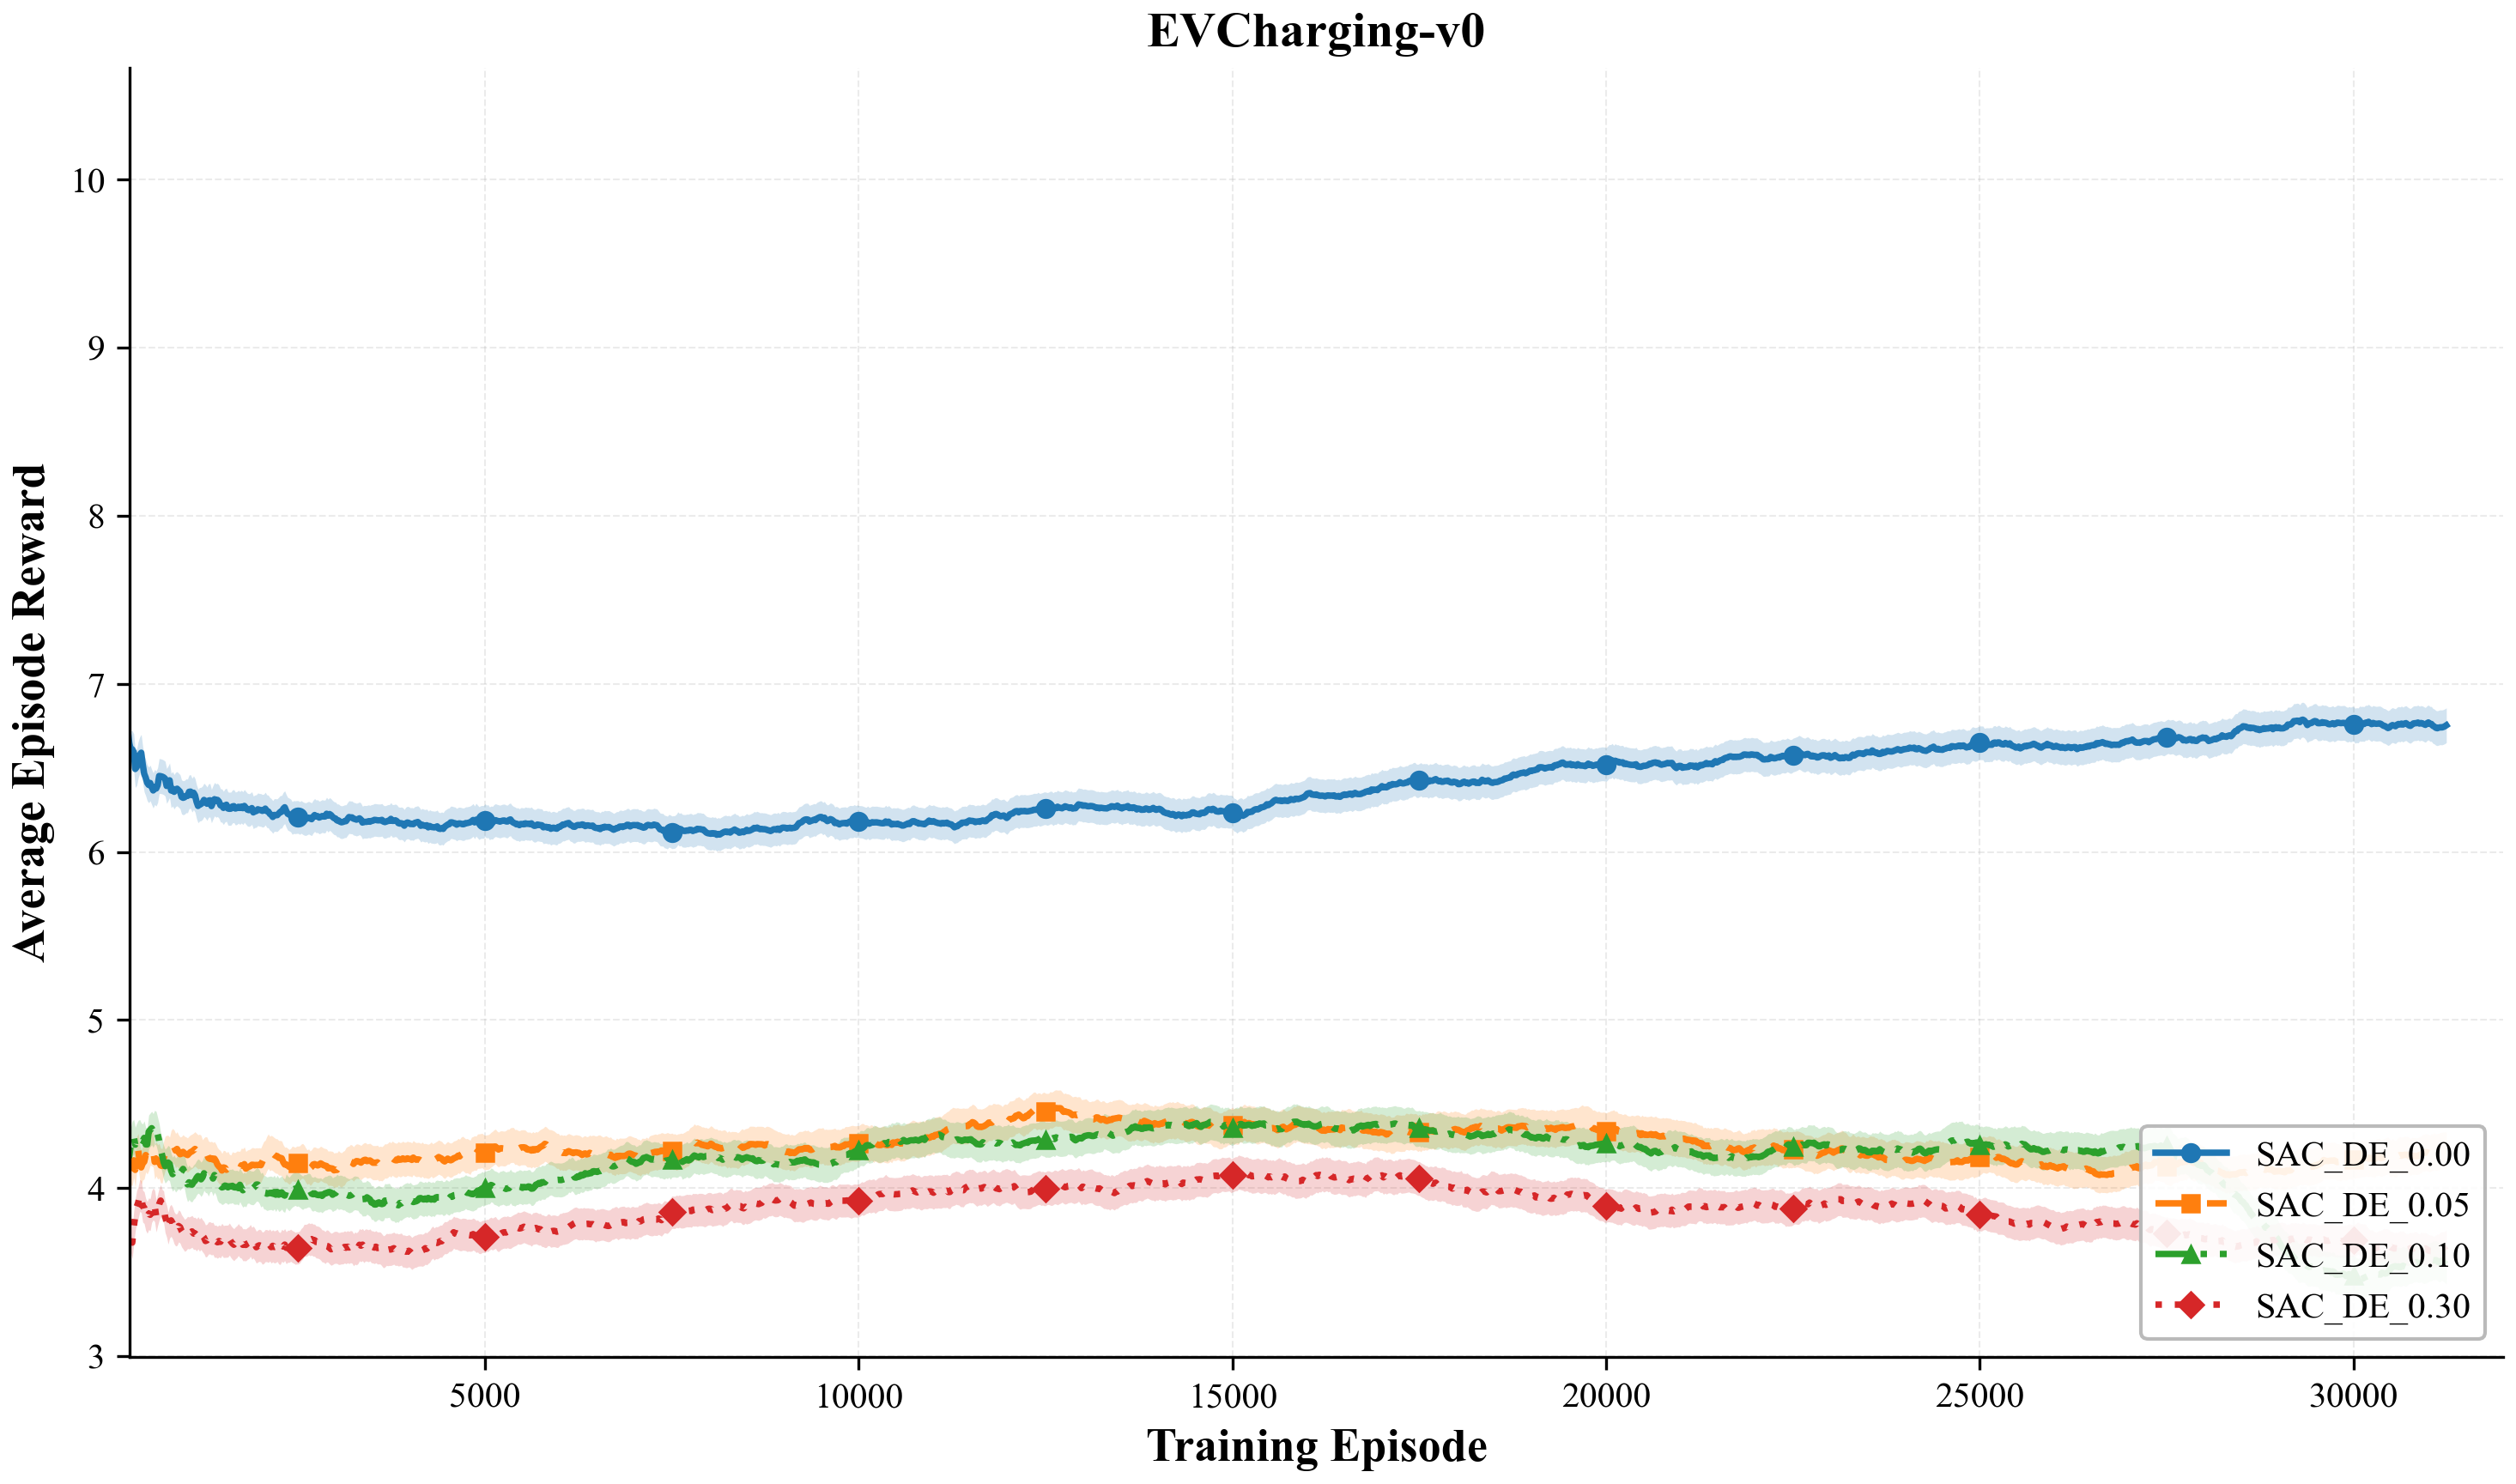
\includegraphics[width=0.9\textwidth]{figures/C_STDRL/ev/SAC/DE_2026-03-16_23-32-10.png}
\caption{EV Charging SAC: Training curves under environment noise (DE).}
\label{fig:stdrl_ev_sac_de}
\end{figure}

\paragraph{Test-time robustness.} Counterintuitively, SAC's performance \emph{improves} under observation noise (\Cref{fig:violin_ev_sac_obs}): the distribution shifts slightly rightward at higher noise levels, suggesting that noise acts as implicit regularization. SAC's entropy-based exploration benefits from additional stochasticity, preventing overfitting to specific EV arrival patterns.

\begin{figure}[htbp]
\centering

\includegraphics[width=0.9\textwidth]{figures/C_POST/evcharging/SAC/obs_violin.png}
\caption{EV Charging SAC: Reward distribution under observation noise. Slight rightward shift at higher noise suggests implicit regularization.}
\label{fig:violin_ev_sac_obs}
\end{figure}

\begin{figure}[htbp]
\centering

\includegraphics[width=0.9\textwidth]{figures/C_POST/evcharging/SAC/action_violin.png}
\caption{EV Charging SAC: Reward distribution under action noise.}
\label{fig:violin_ev_sac_act}
\end{figure}

\begin{figure}[htbp]
\centering

\includegraphics[width=0.9\textwidth]{figures/C_POST/evcharging/SAC/env_violin.png}
\caption{EV Charging SAC: Reward distribution under environment noise. Distribution broadens at high noise, indicating increased episode-to-episode variability in MOER-dependent rewards.}
\label{fig:violin_ev_sac_env}
\end{figure}

\begin{figure}[htbp]
\centering

\includegraphics[width=0.9\textwidth]{figures/C_POST/evcharging/SAC/panel.png}
\caption{EV Charging SAC: Summary panel across all three noise channels.}
\label{fig:post_ev_sac_panel}
\end{figure}

% ============================================================
\subsection{Building: Noise Robustness}
\label{sec:noise_bu}

The Building environment is the most noise-sensitive of the three environments, with rapid performance degradation under observation and environment noise. The RC thermal model amplifies per-timestep observation errors through coupled zone dynamics, creating cascading failures over the 288-step episode.

% --- Building PPO ---
\subsubsection{Building --- PPO}

\paragraph{Training curves.} \Cref{fig:stdrl_bu_ppo_ds} shows a clear separation between noise levels during training: higher observation noise leads to lower converged reward. Action noise (\Cref{fig:stdrl_bu_ppo_da}) and environment noise (\Cref{fig:stdrl_bu_ppo_de}) show similar but more severe training degradation patterns.

\begin{figure}[htbp]
\centering
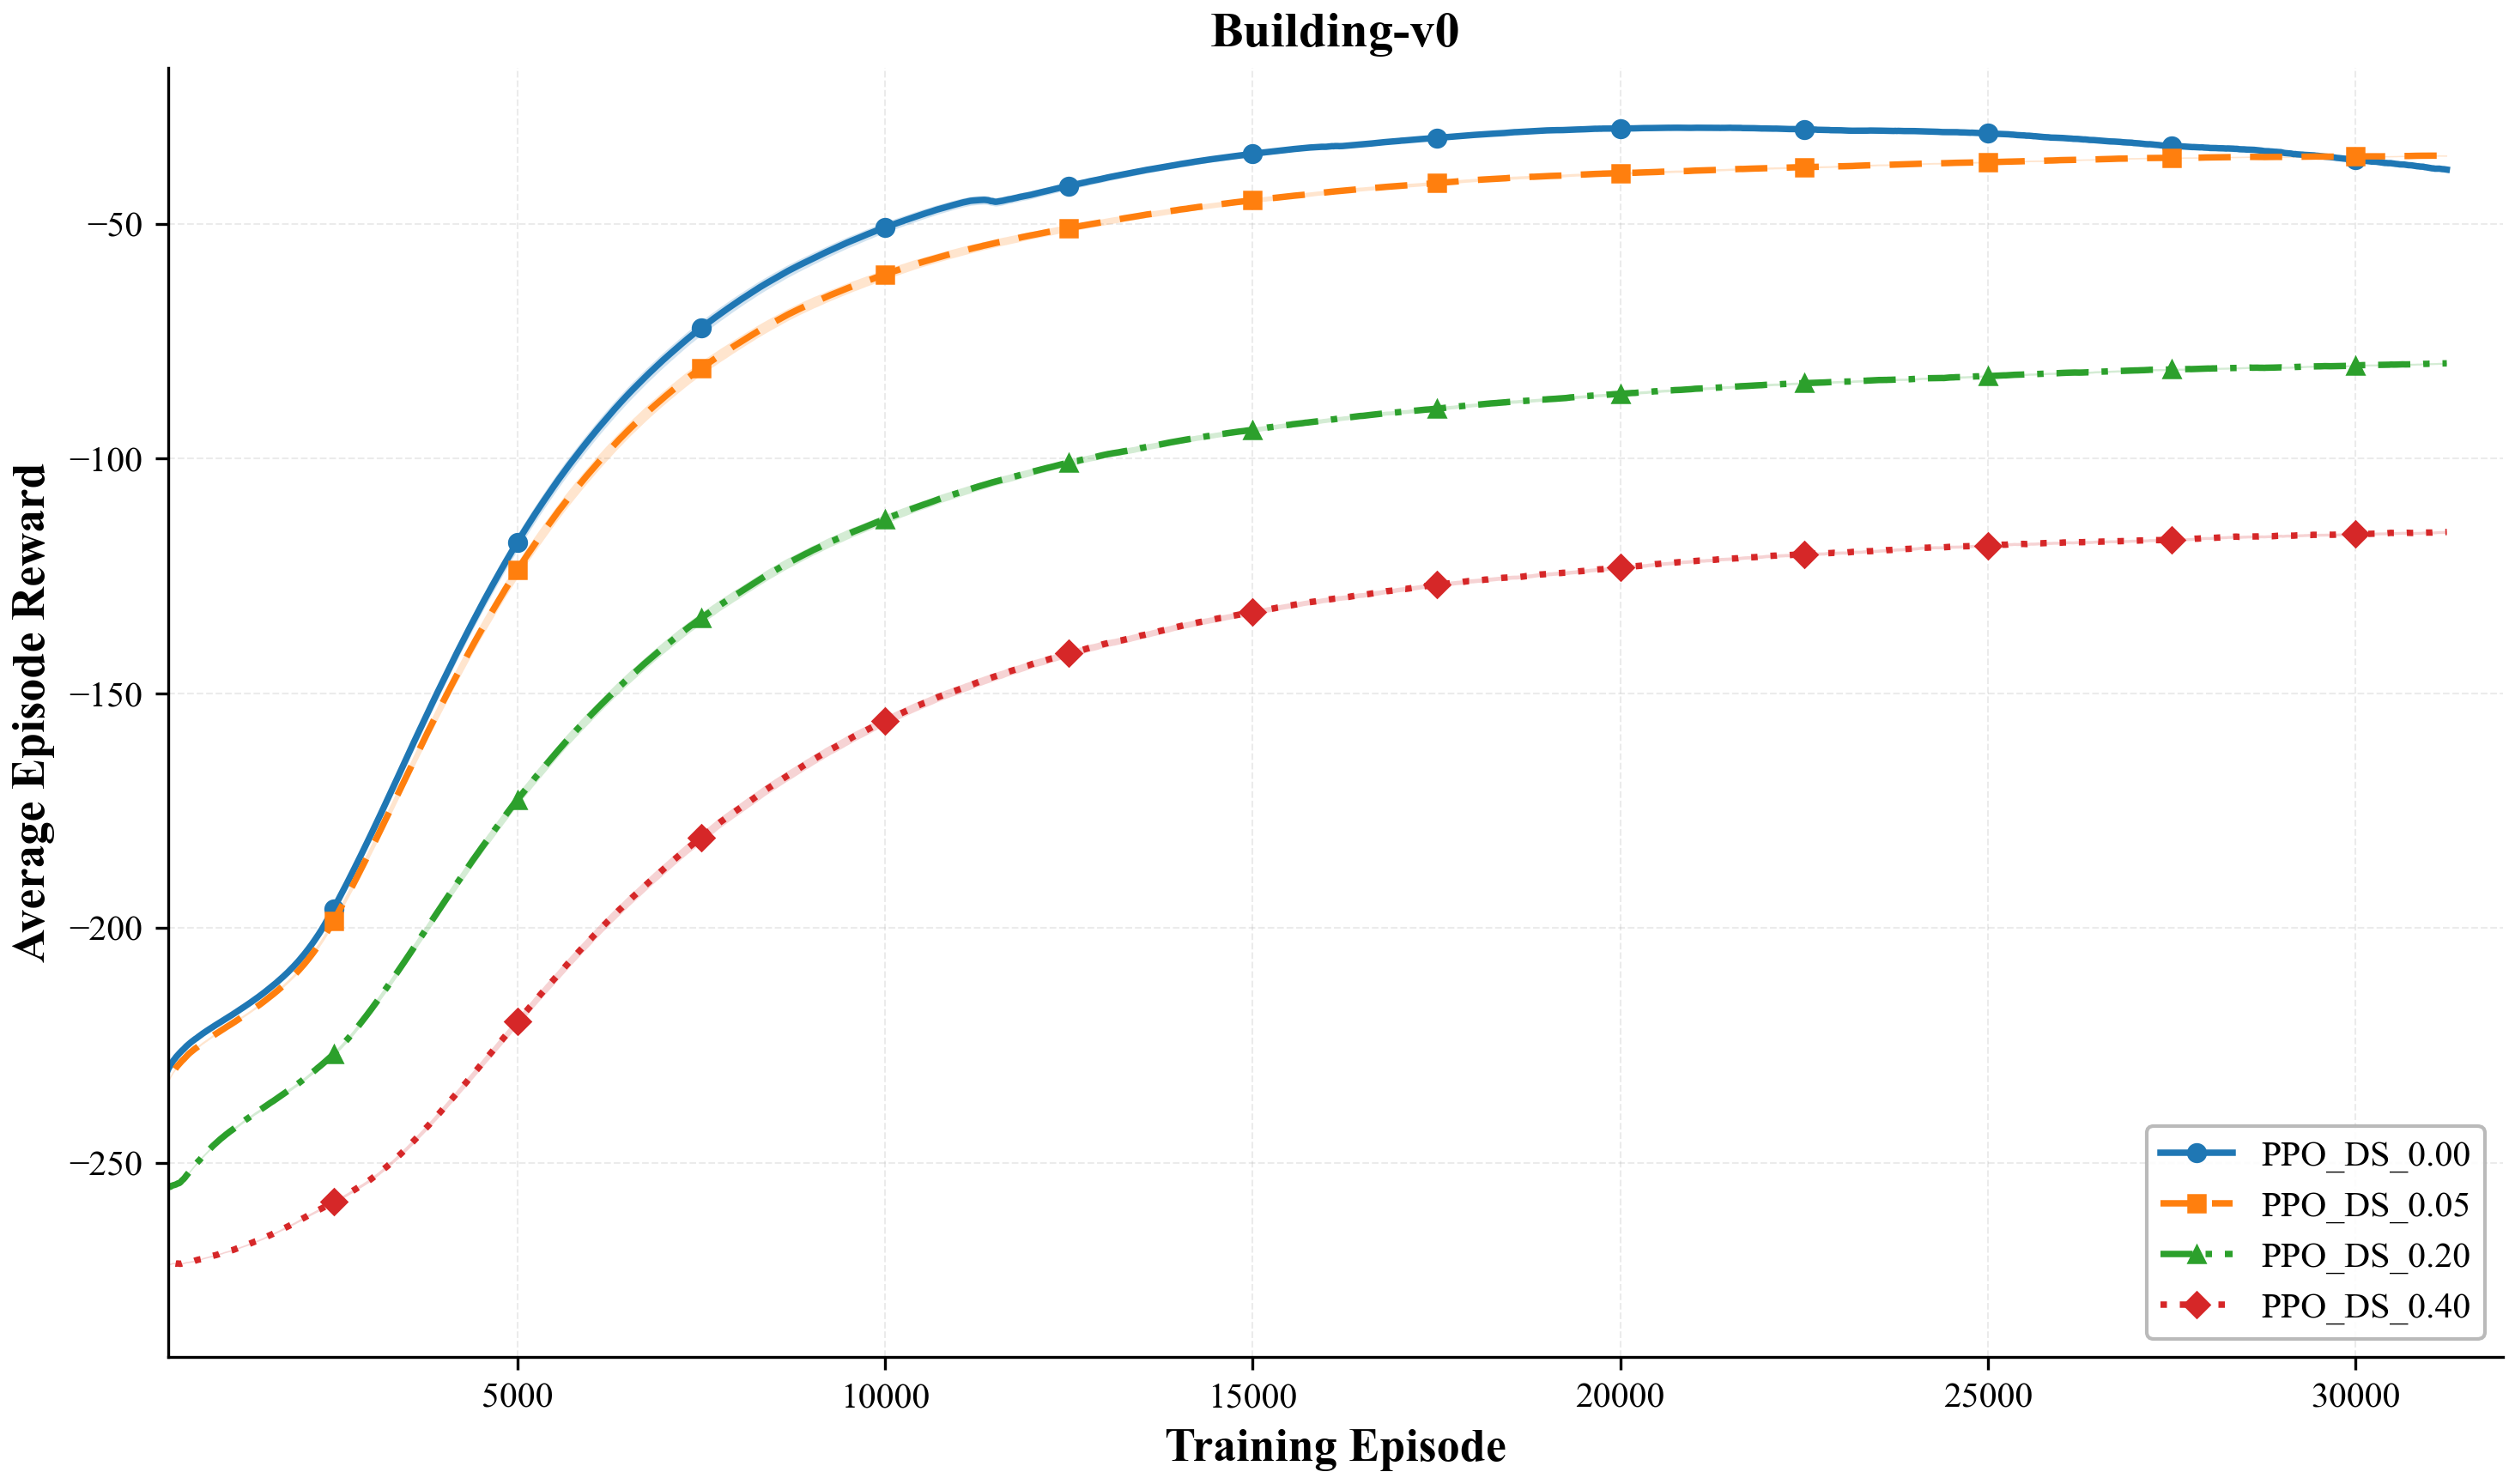
\includegraphics[width=0.9\textwidth]{figures/C_STDRL/bu/PPO/DS_2026-03-16_23-32-18.png}
\caption{Building PPO: Training curves under observation noise (DS).}
\label{fig:stdrl_bu_ppo_ds}
\end{figure}

\begin{figure}[htbp]
\centering
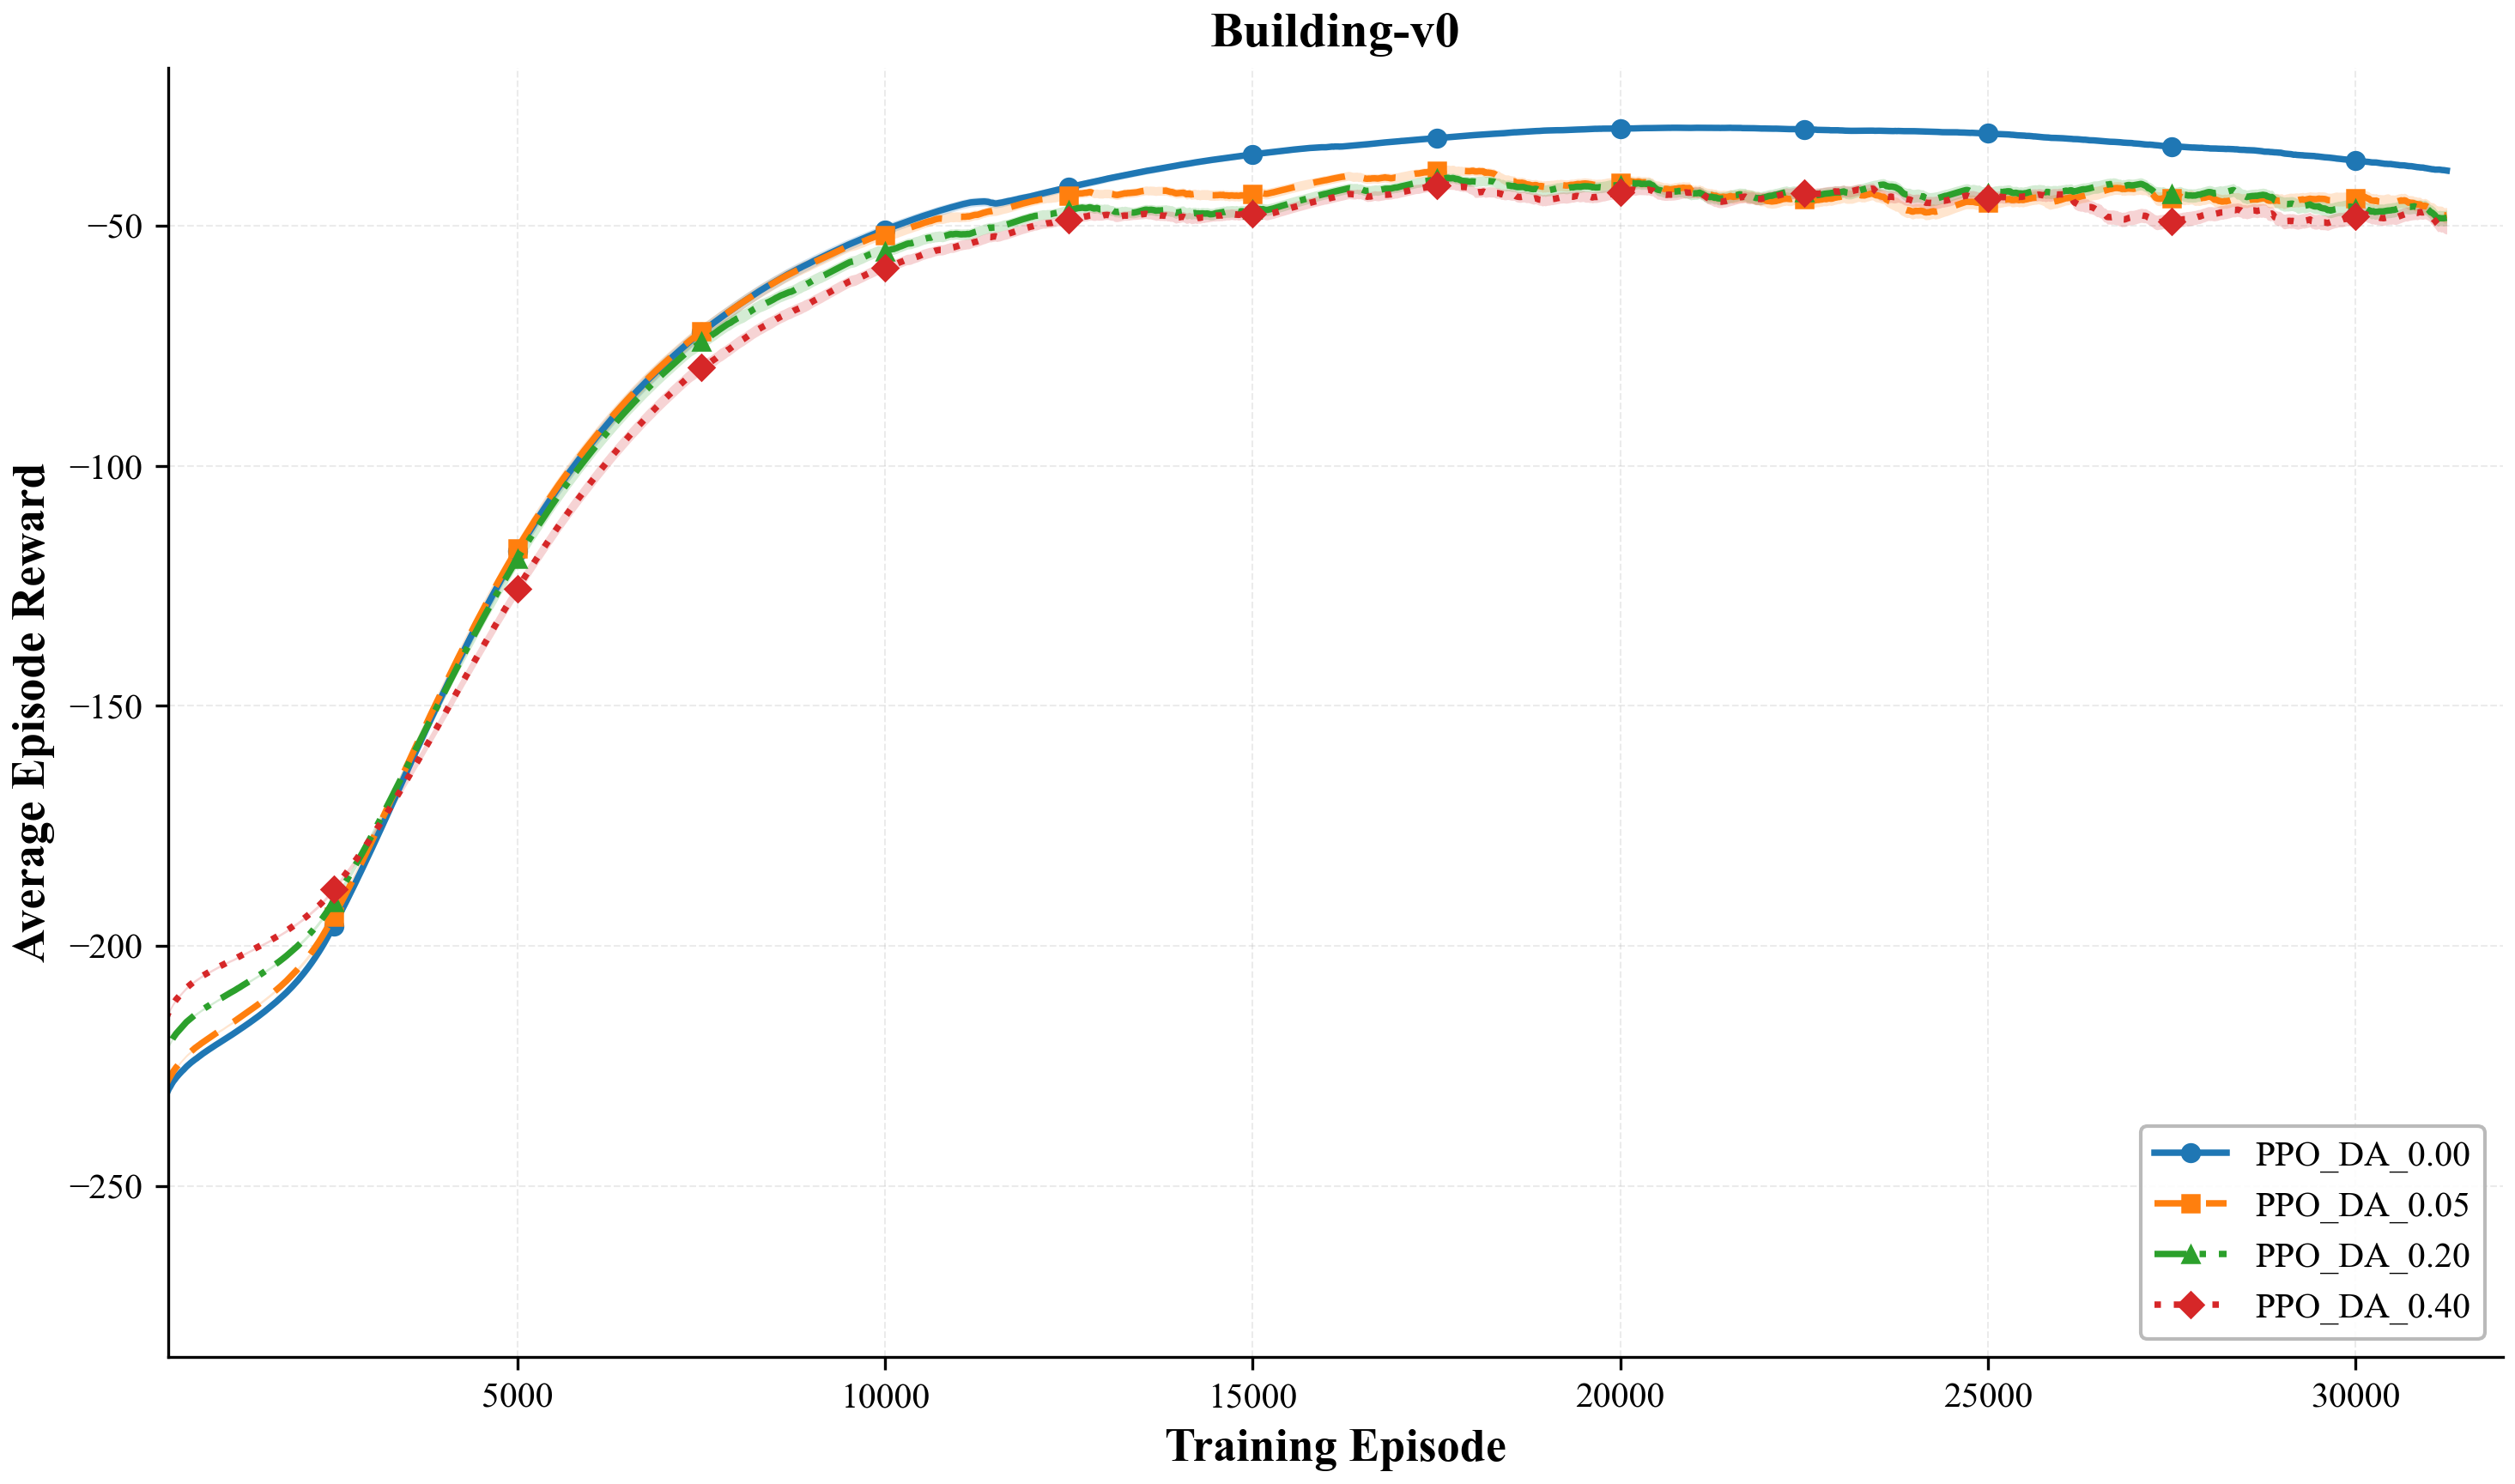
\includegraphics[width=0.9\textwidth]{figures/C_STDRL/bu/PPO/DA_2026-03-16_23-32-19.png}
\caption{Building PPO: Training curves under action noise (DA).}
\label{fig:stdrl_bu_ppo_da}
\end{figure}

\begin{figure}[htbp]
\centering
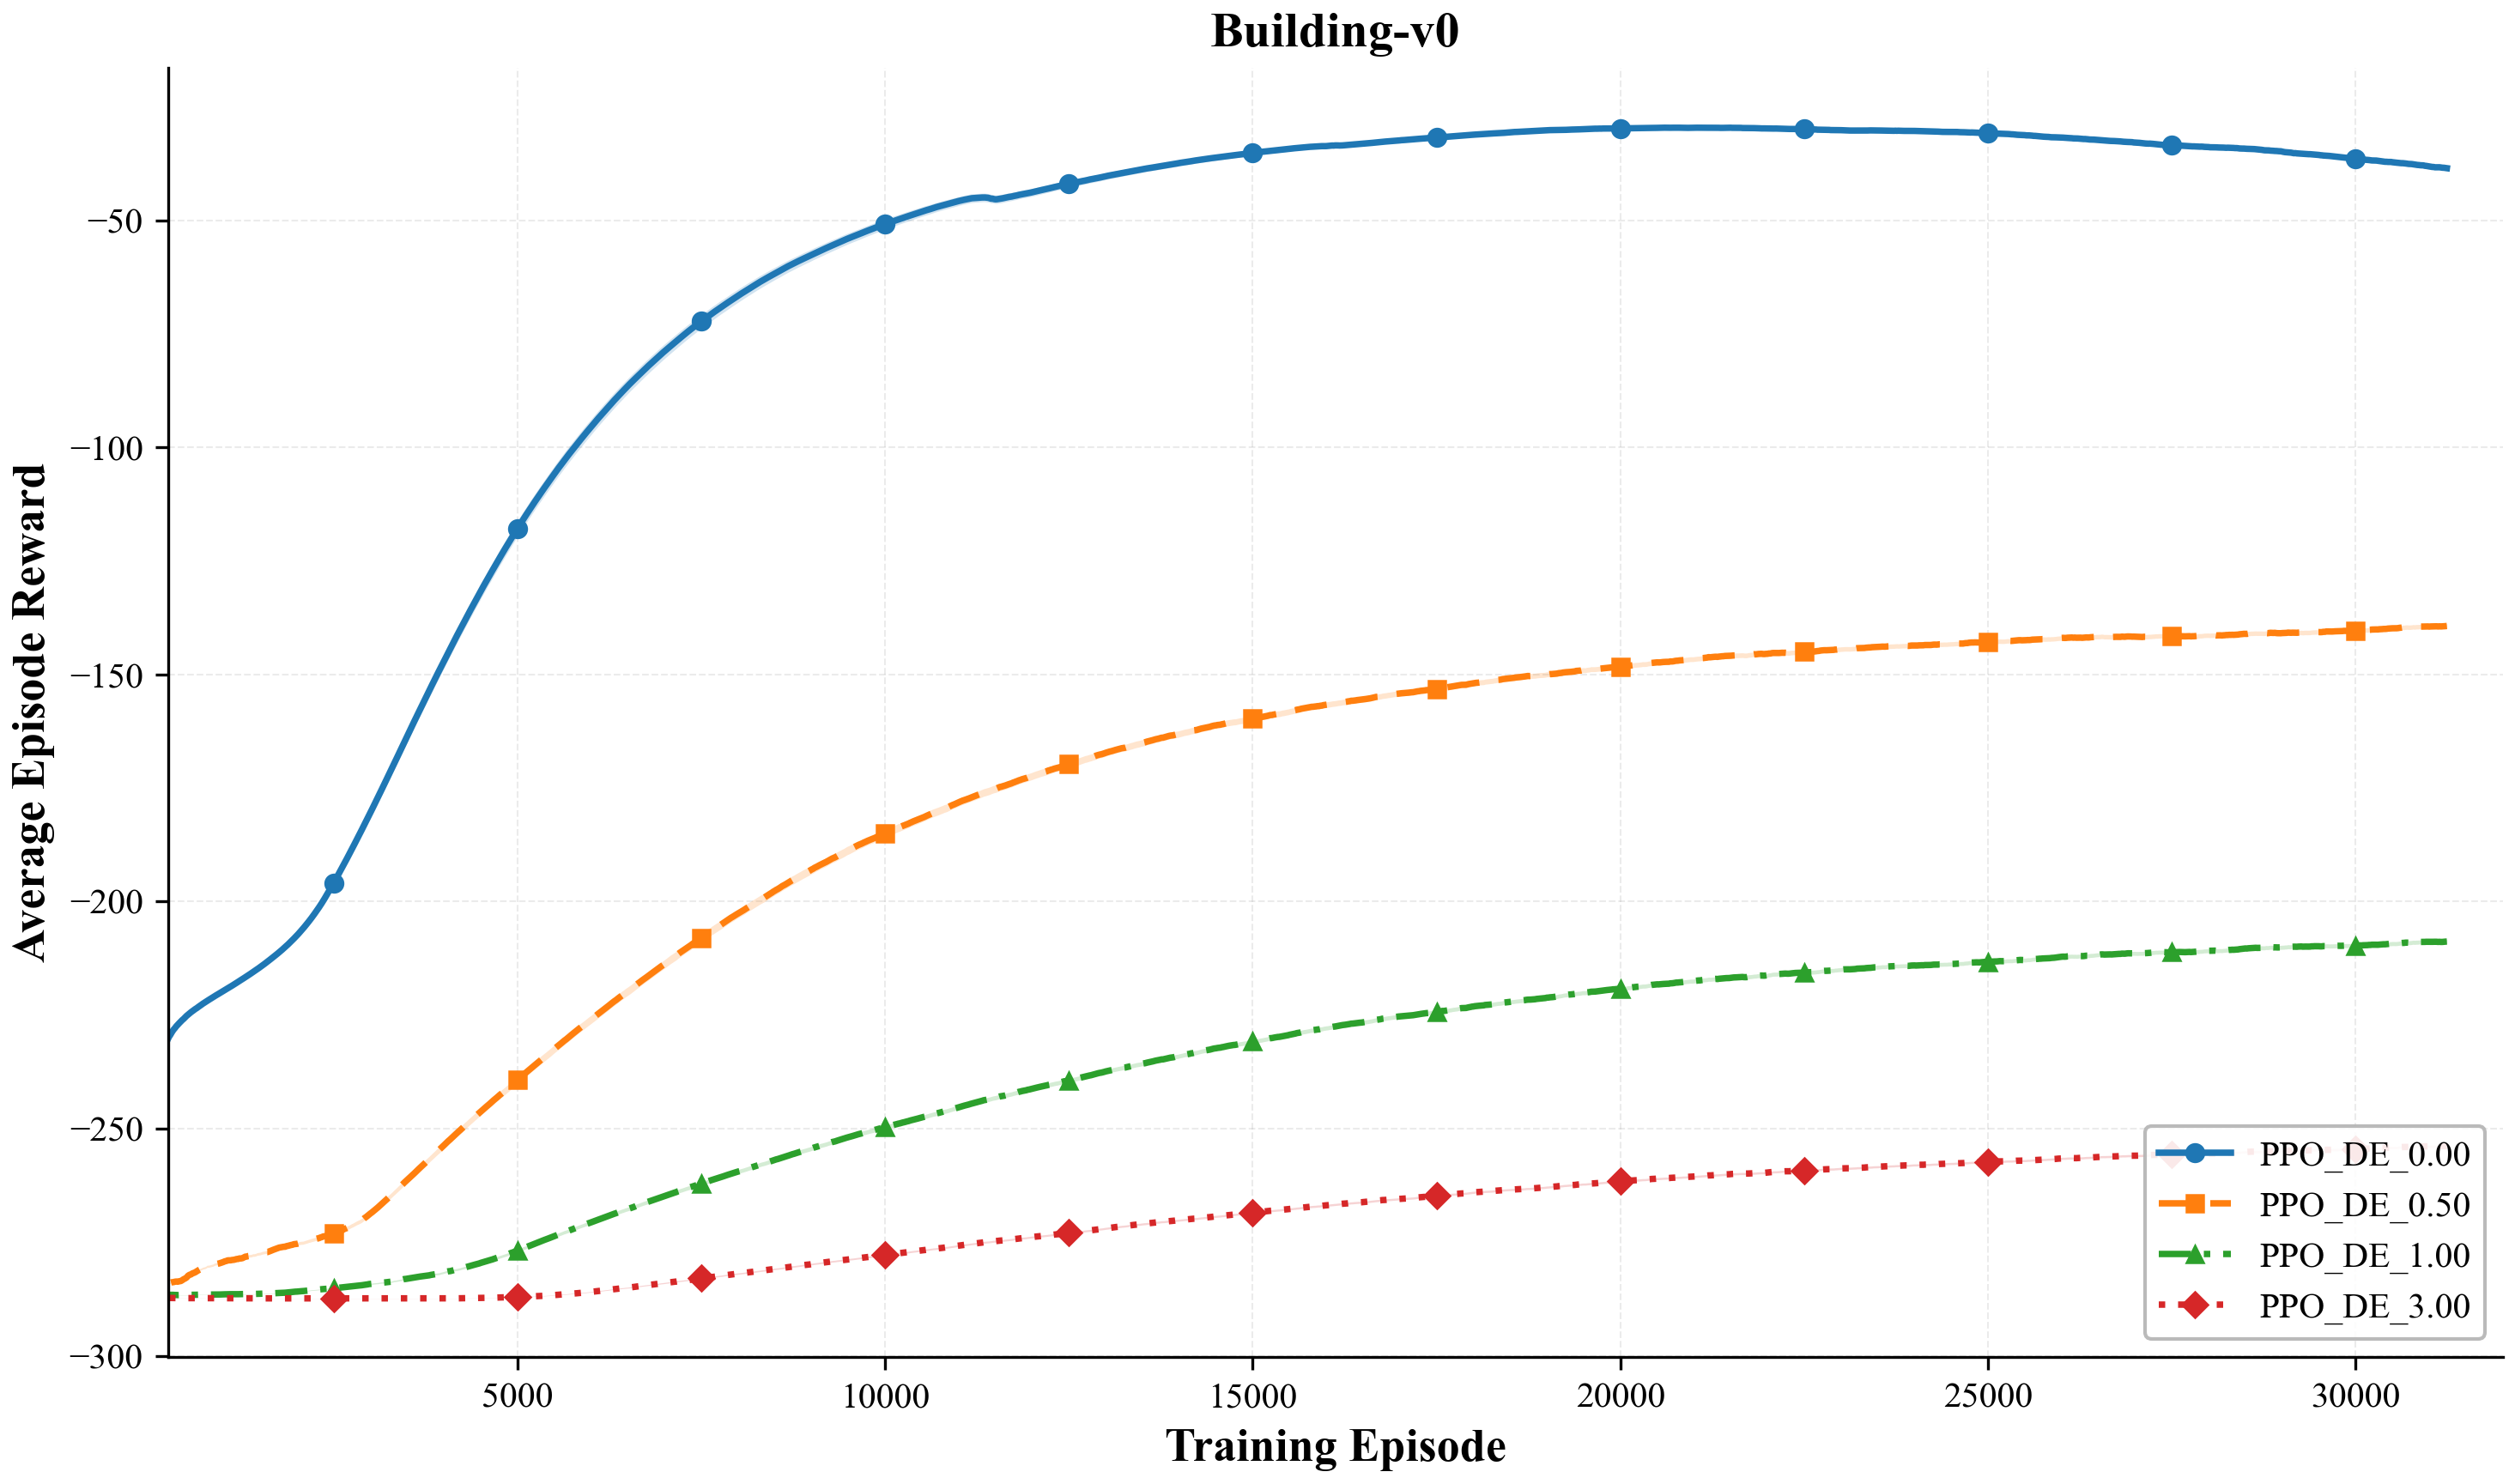
\includegraphics[width=0.9\textwidth]{figures/C_STDRL/bu/PPO/DE_2026-03-16_23-32-21.png}
\caption{Building PPO: Training curves under environment noise (DE).}
\label{fig:stdrl_bu_ppo_de}
\end{figure}

\paragraph{Test-time robustness.} The violin plots reveal the distributional impact of noise. Under observation noise (\Cref{fig:violin_bu_ppo_obs}), the bimodal reward structure---driven by high-occupancy vs.\ low-occupancy days---shifts entirely downward at $\sigma \geq 0.15$, with the high-reward mode collapsing. Under action noise (\Cref{fig:violin_bu_ppo_act}), the distribution shape is largely preserved up to $\sigma_{\text{act}} = 0.2$, consistent with the HVAC system's bang-bang control nature. Under environment noise (\Cref{fig:violin_bu_ppo_env}), the entire distribution collapses catastrophically as thermal dynamics amplify weather prediction errors.

\begin{figure}[htbp]
\centering
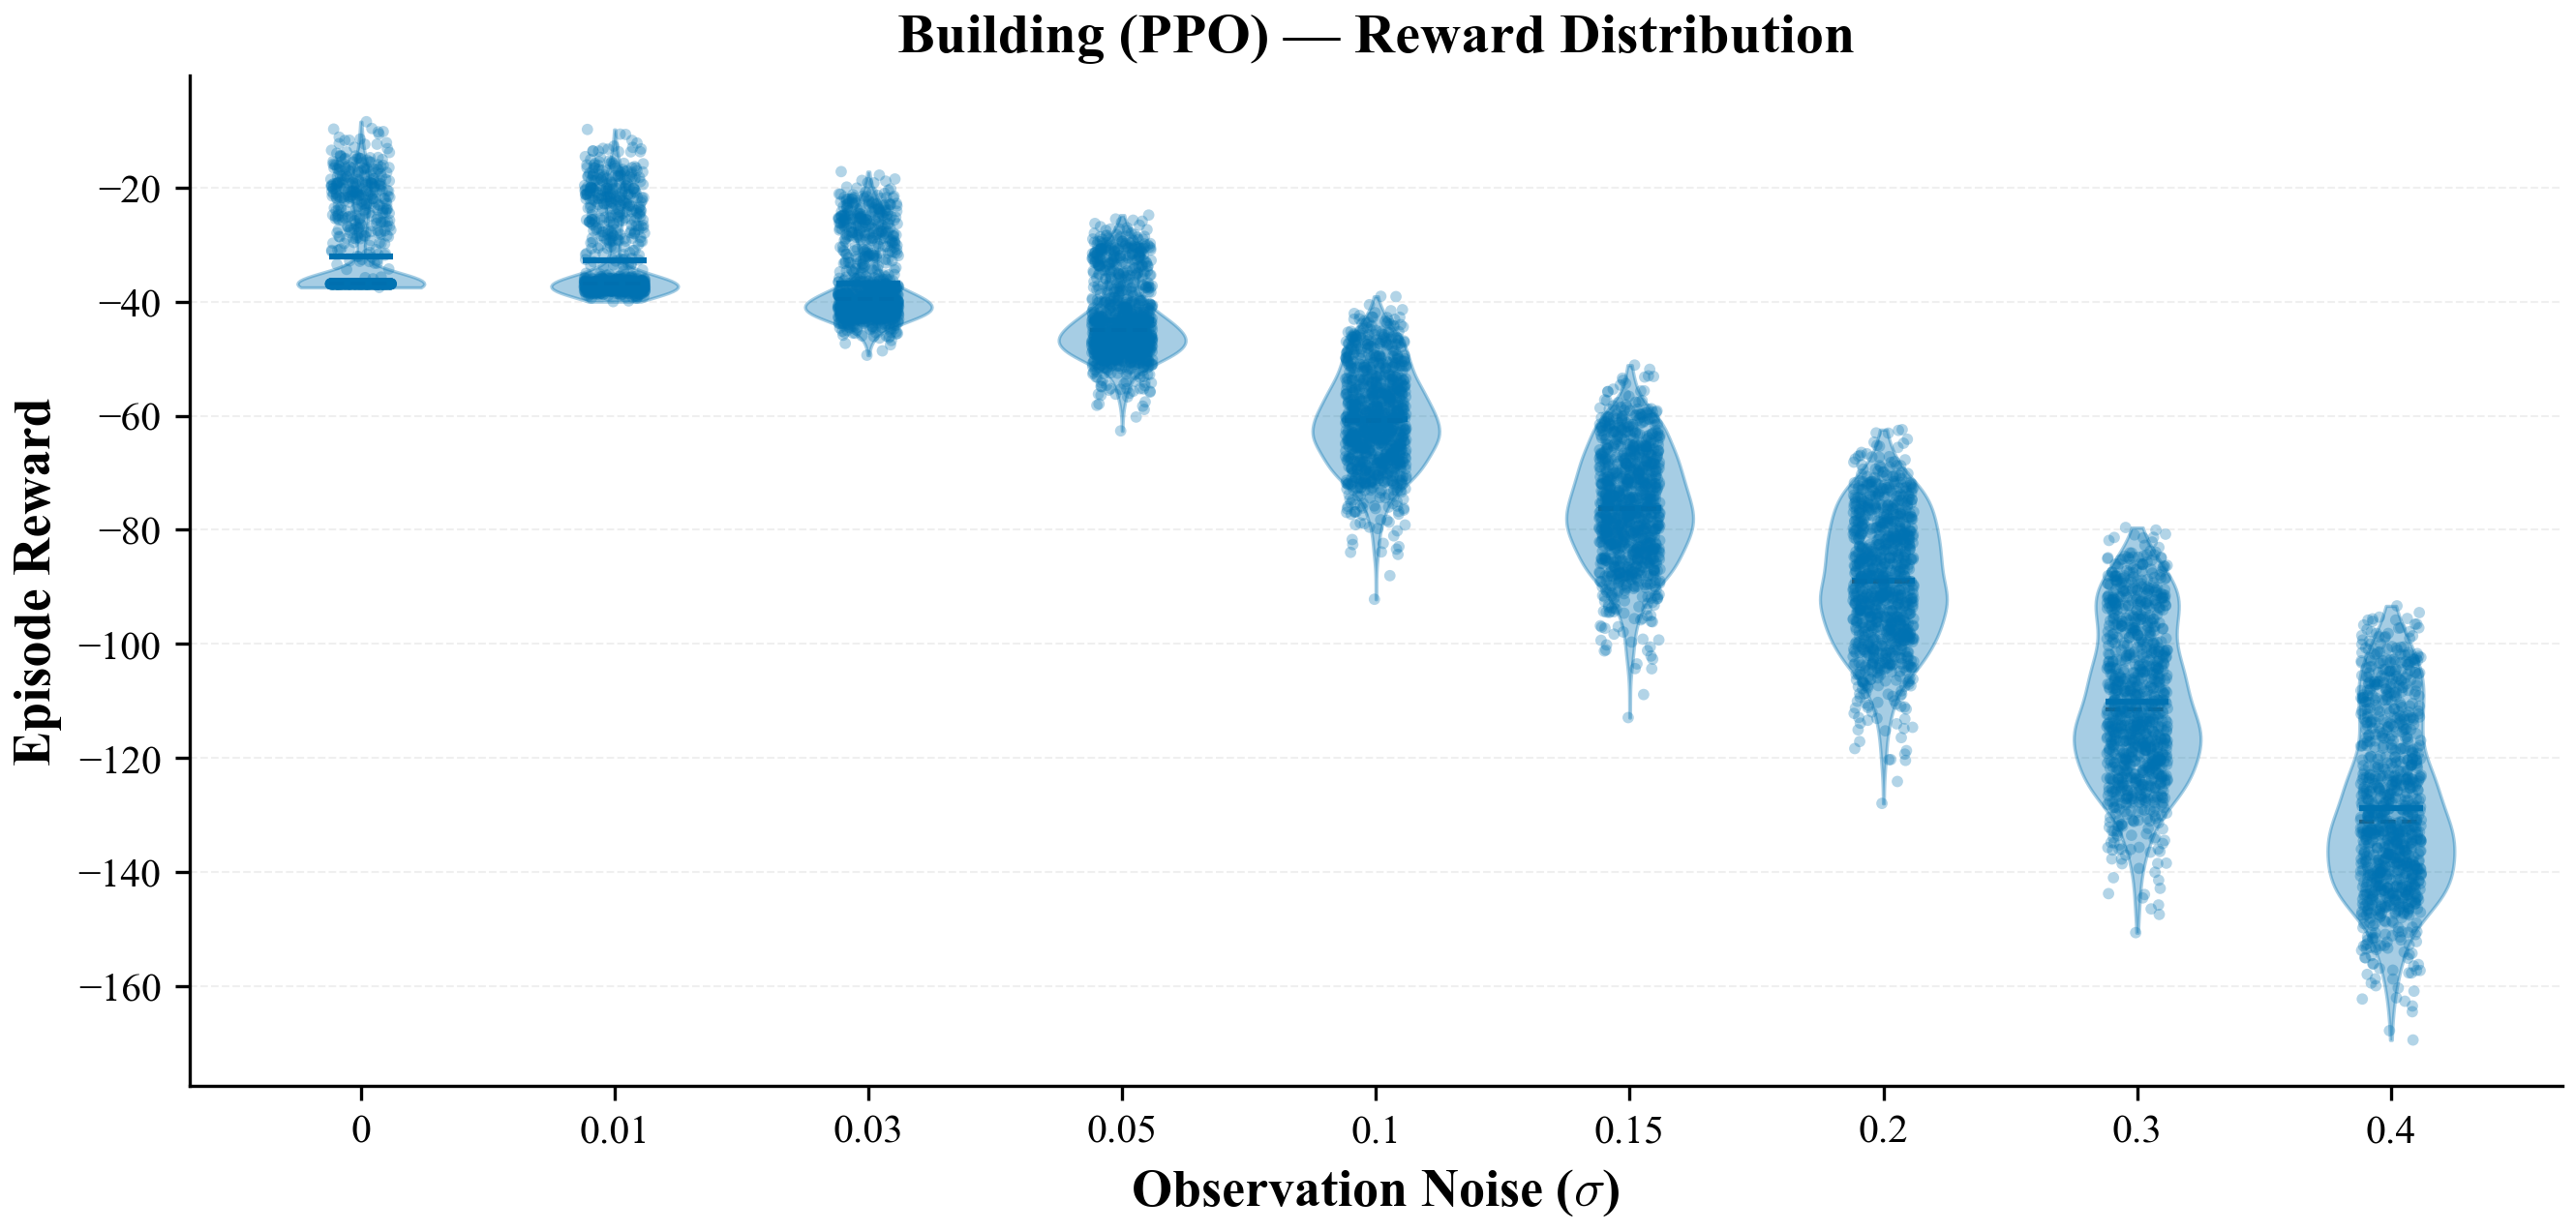
\includegraphics[width=0.9\textwidth]{figures/C_POST/building/PPO/obs_violin.png}
\caption{Building PPO: Reward distribution under observation noise. The bimodal structure shifts downward with increasing noise; the high-reward mode collapses at $\sigma \geq 0.15$.}
\label{fig:violin_bu_ppo_obs}
\end{figure}

\begin{figure}[htbp]
\centering
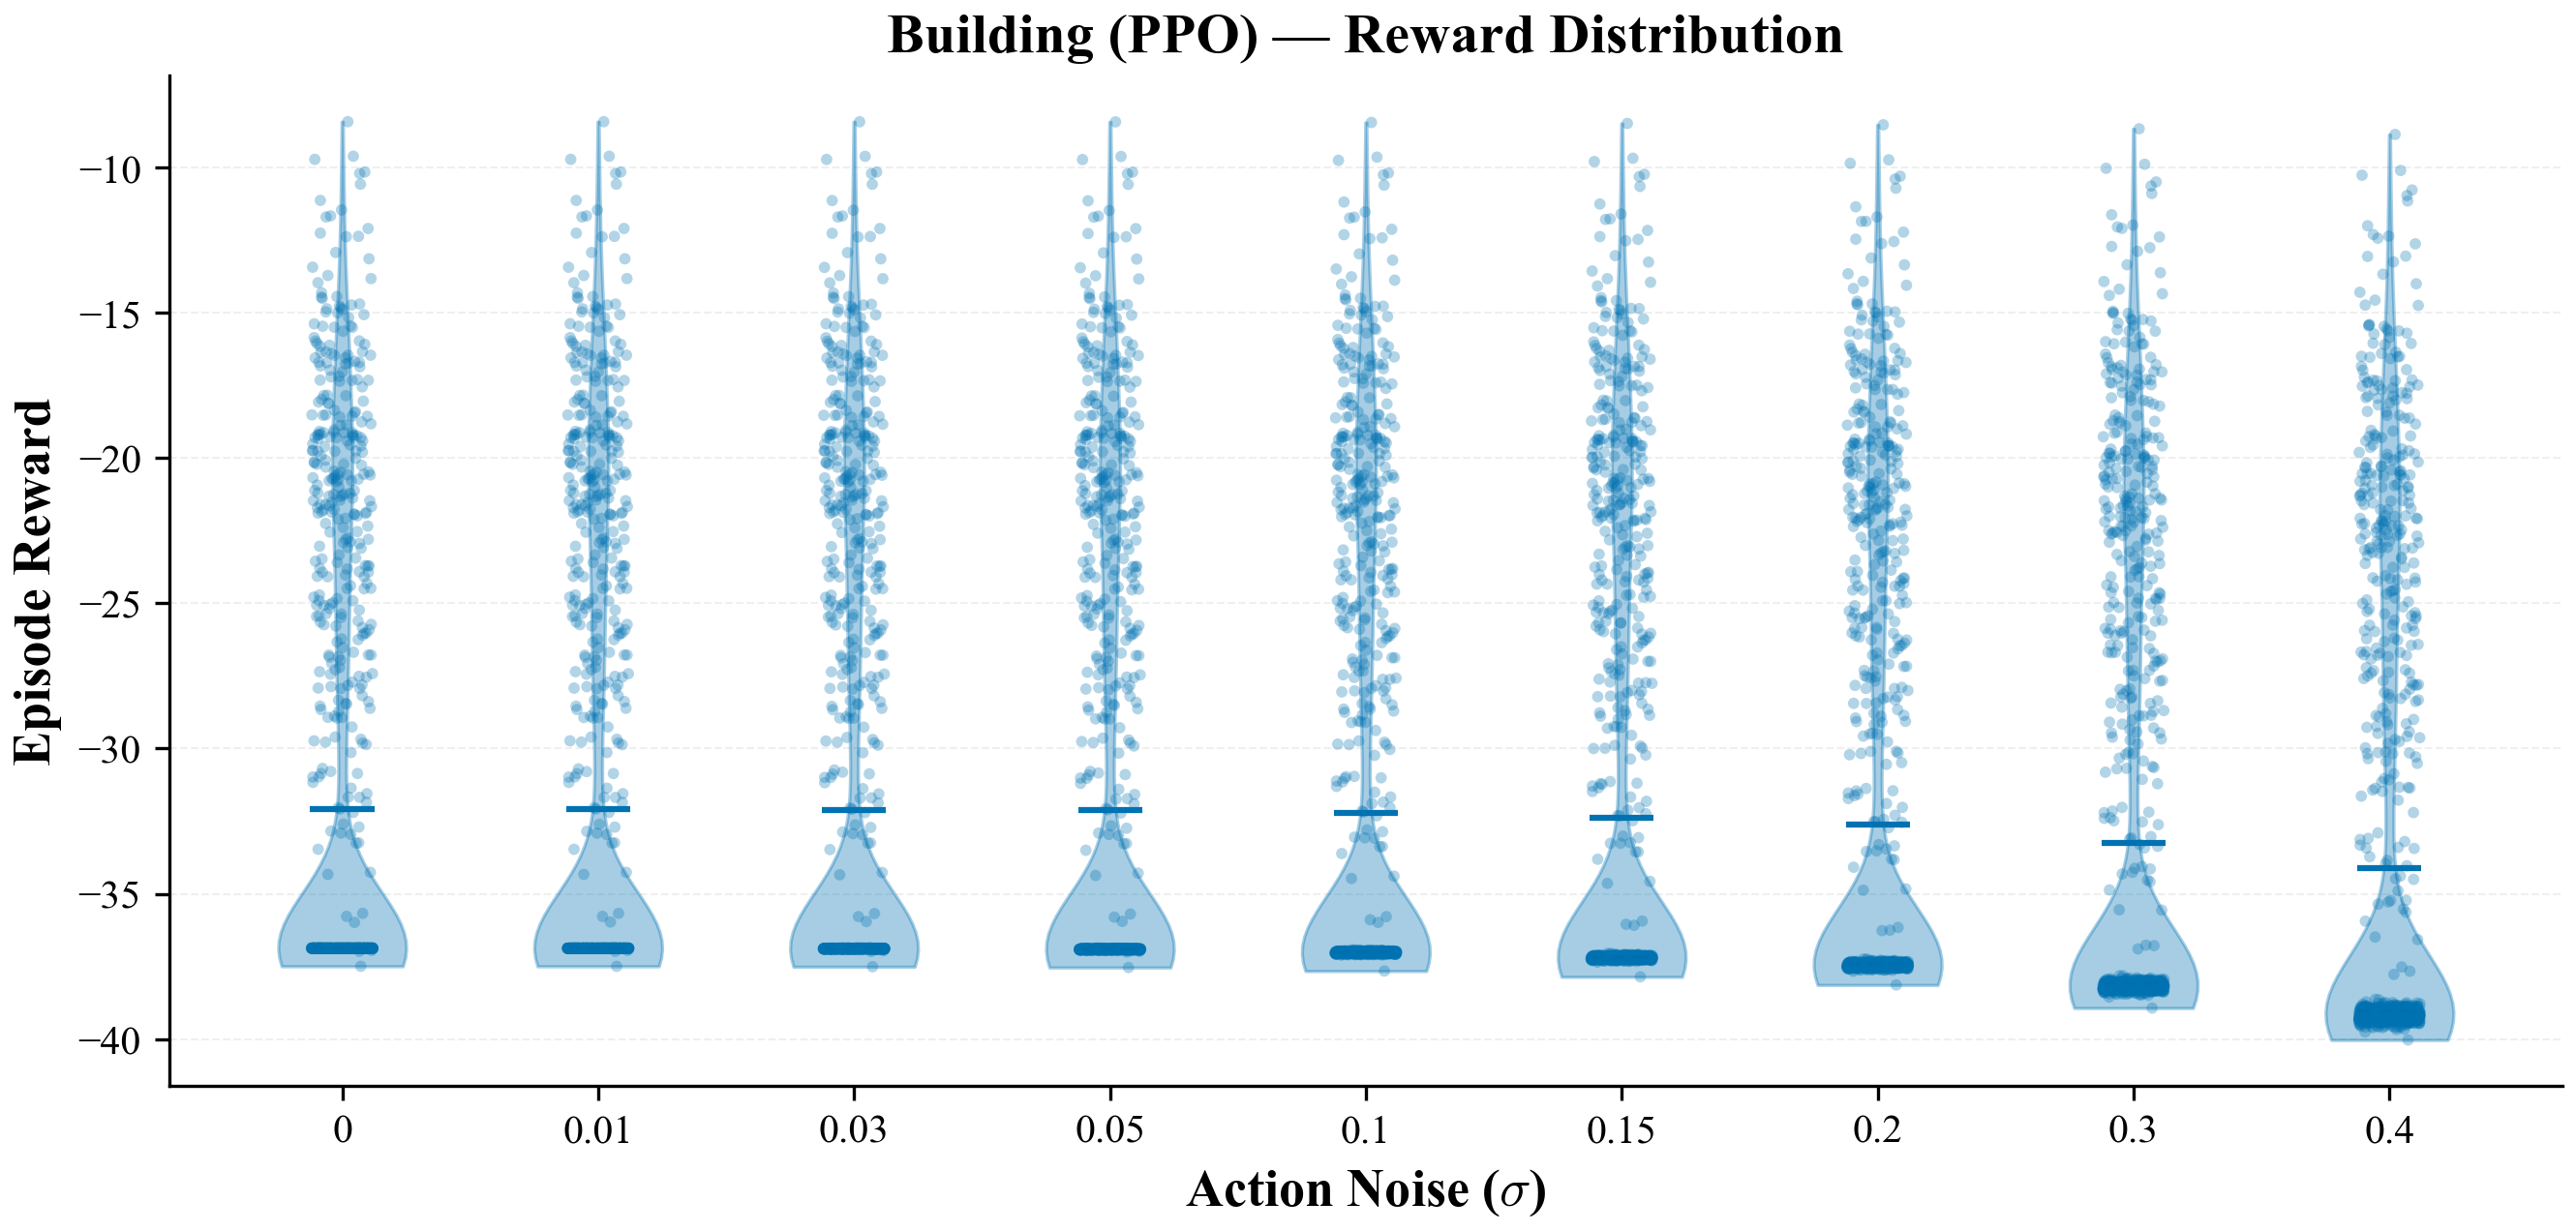
\includegraphics[width=0.9\textwidth]{figures/C_POST/building/PPO/action_violin.png}
\caption{Building PPO: Reward distribution under action noise. Distribution shape preserved up to $\sigma_{\text{act}} = 0.2$, consistent with bang-bang HVAC control.}
\label{fig:violin_bu_ppo_act}
\end{figure}

\begin{figure}[htbp]
\centering
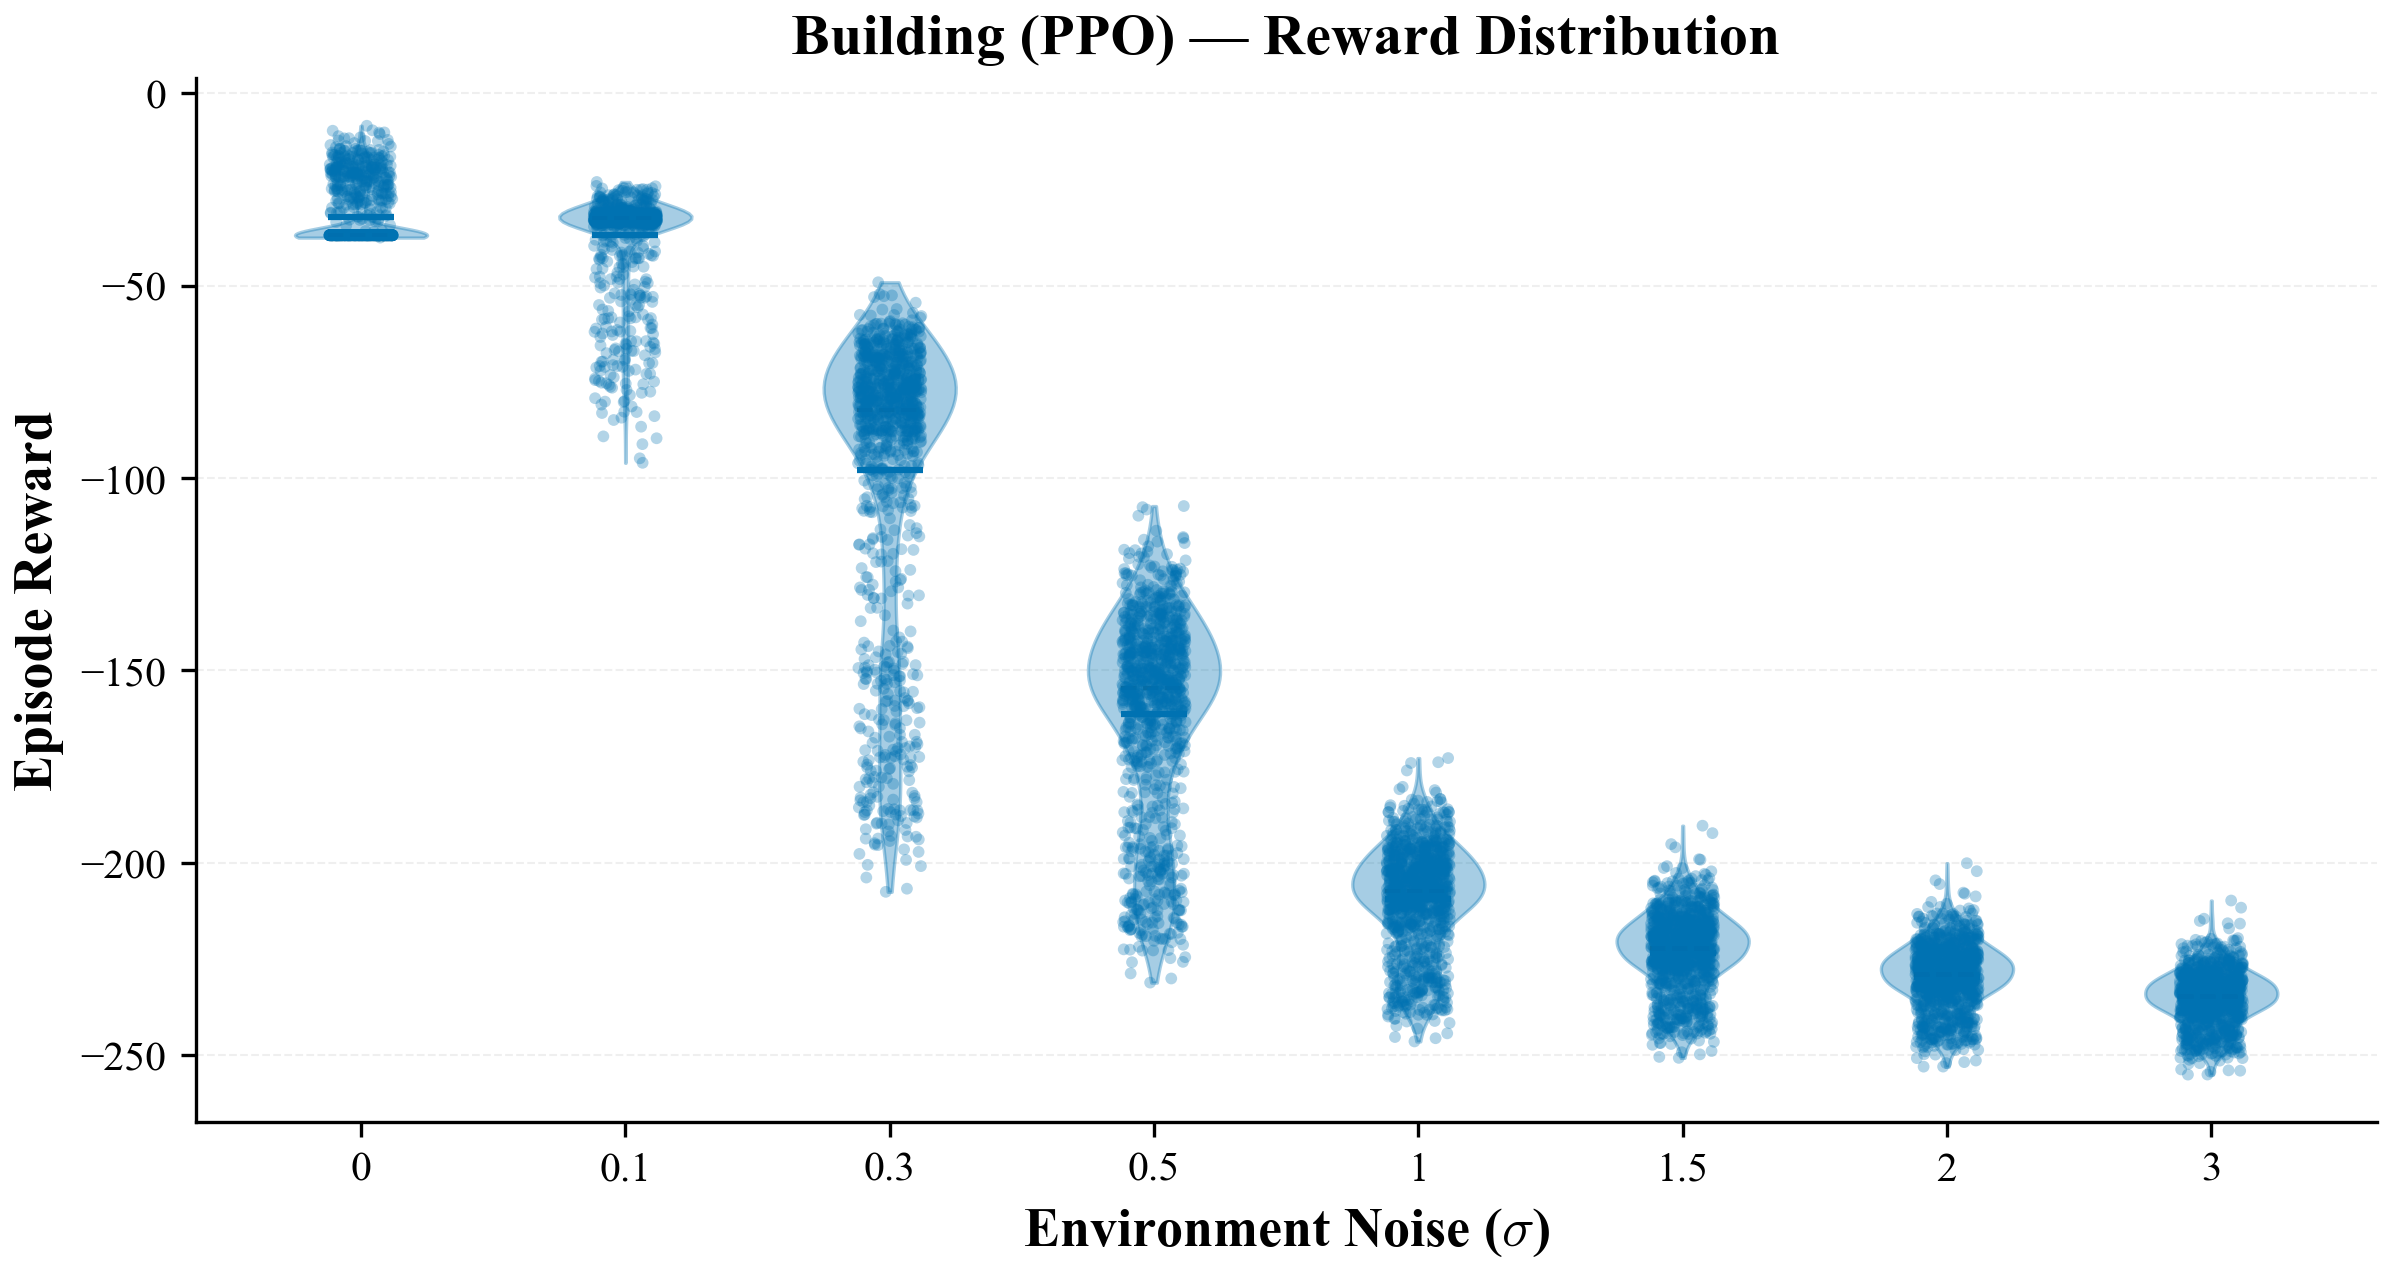
\includegraphics[width=0.9\textwidth]{figures/C_POST/building/PPO/env_violin.png}
\caption{Building PPO: Reward distribution under environment noise. Catastrophic degradation: the entire distribution collapses as thermal dynamics amplify weather prediction errors.}
\label{fig:violin_bu_ppo_env}
\end{figure}

\begin{figure}[htbp]
\centering
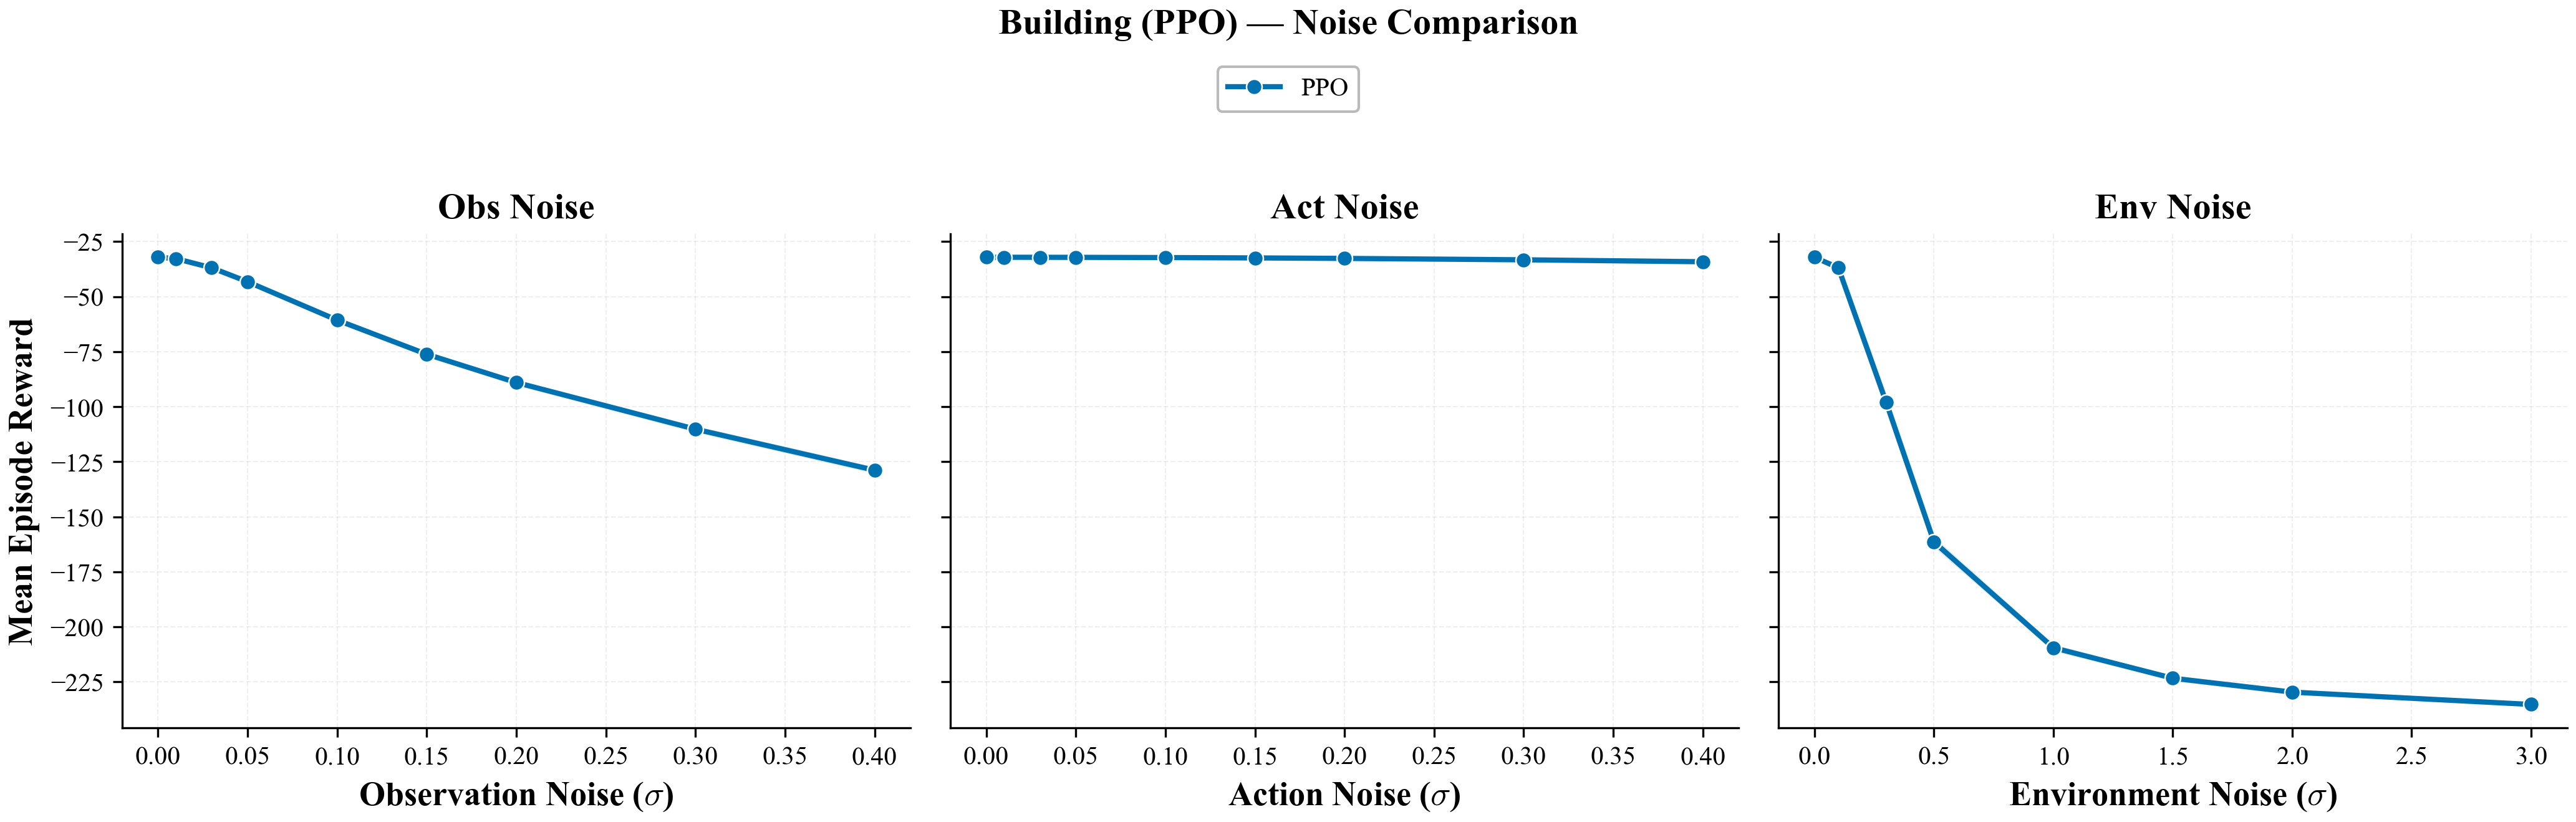
\includegraphics[width=0.9\textwidth]{figures/C_POST/building/PPO/panel.png}
\caption{Building PPO: Summary panel. Observation and environment noise cause severe degradation; action noise has minimal impact.}
\label{fig:post_bu_ppo_panel}
\end{figure}

% --- Building SAC ---
\subsubsection{Building --- SAC}

\paragraph{Training curves.} SAC's training curves (\Cref{fig:stdrl_bu_sac_ds,fig:stdrl_bu_sac_da,fig:stdrl_bu_sac_de}) show a similar pattern to PPO but with lower absolute performance due to SAC's weaker baseline in this environment.

\begin{figure}[htbp]
\centering
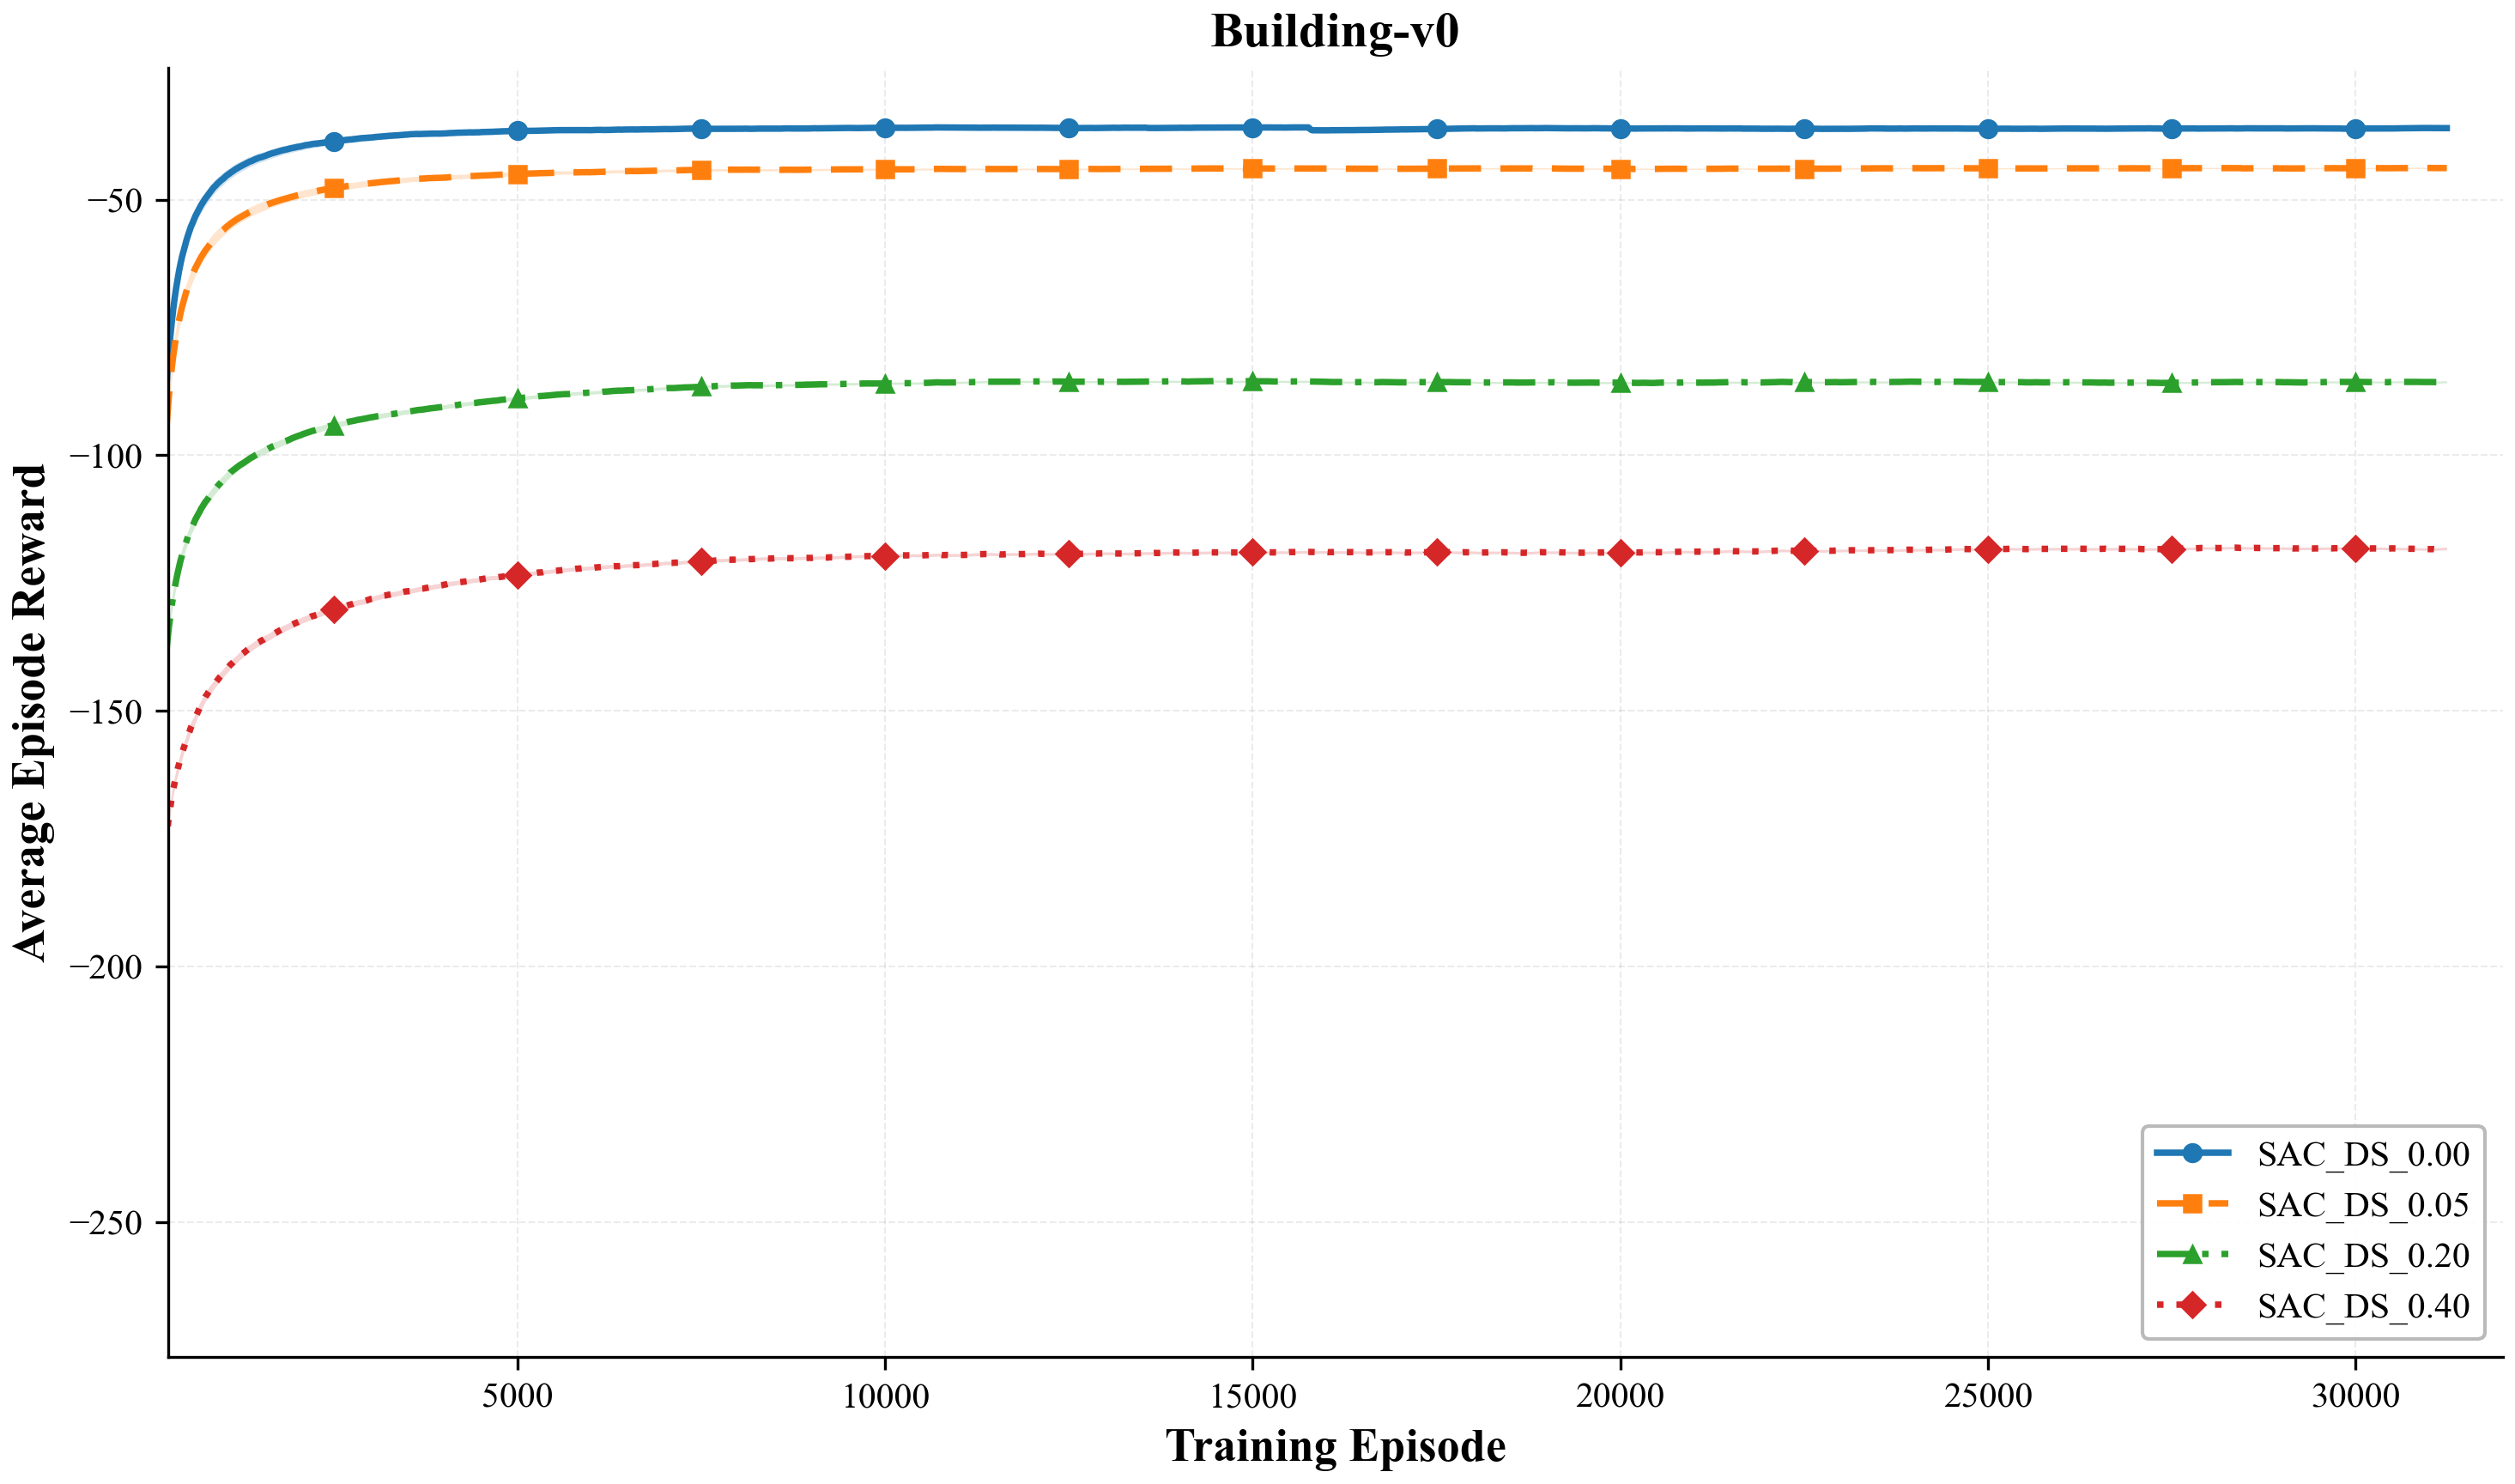
\includegraphics[width=0.9\textwidth]{figures/C_STDRL/bu/SAC/DS_2026-03-16_23-32-23.png}
\caption{Building SAC: Training curves under observation noise (DS).}
\label{fig:stdrl_bu_sac_ds}
\end{figure}

\begin{figure}[htbp]
\centering
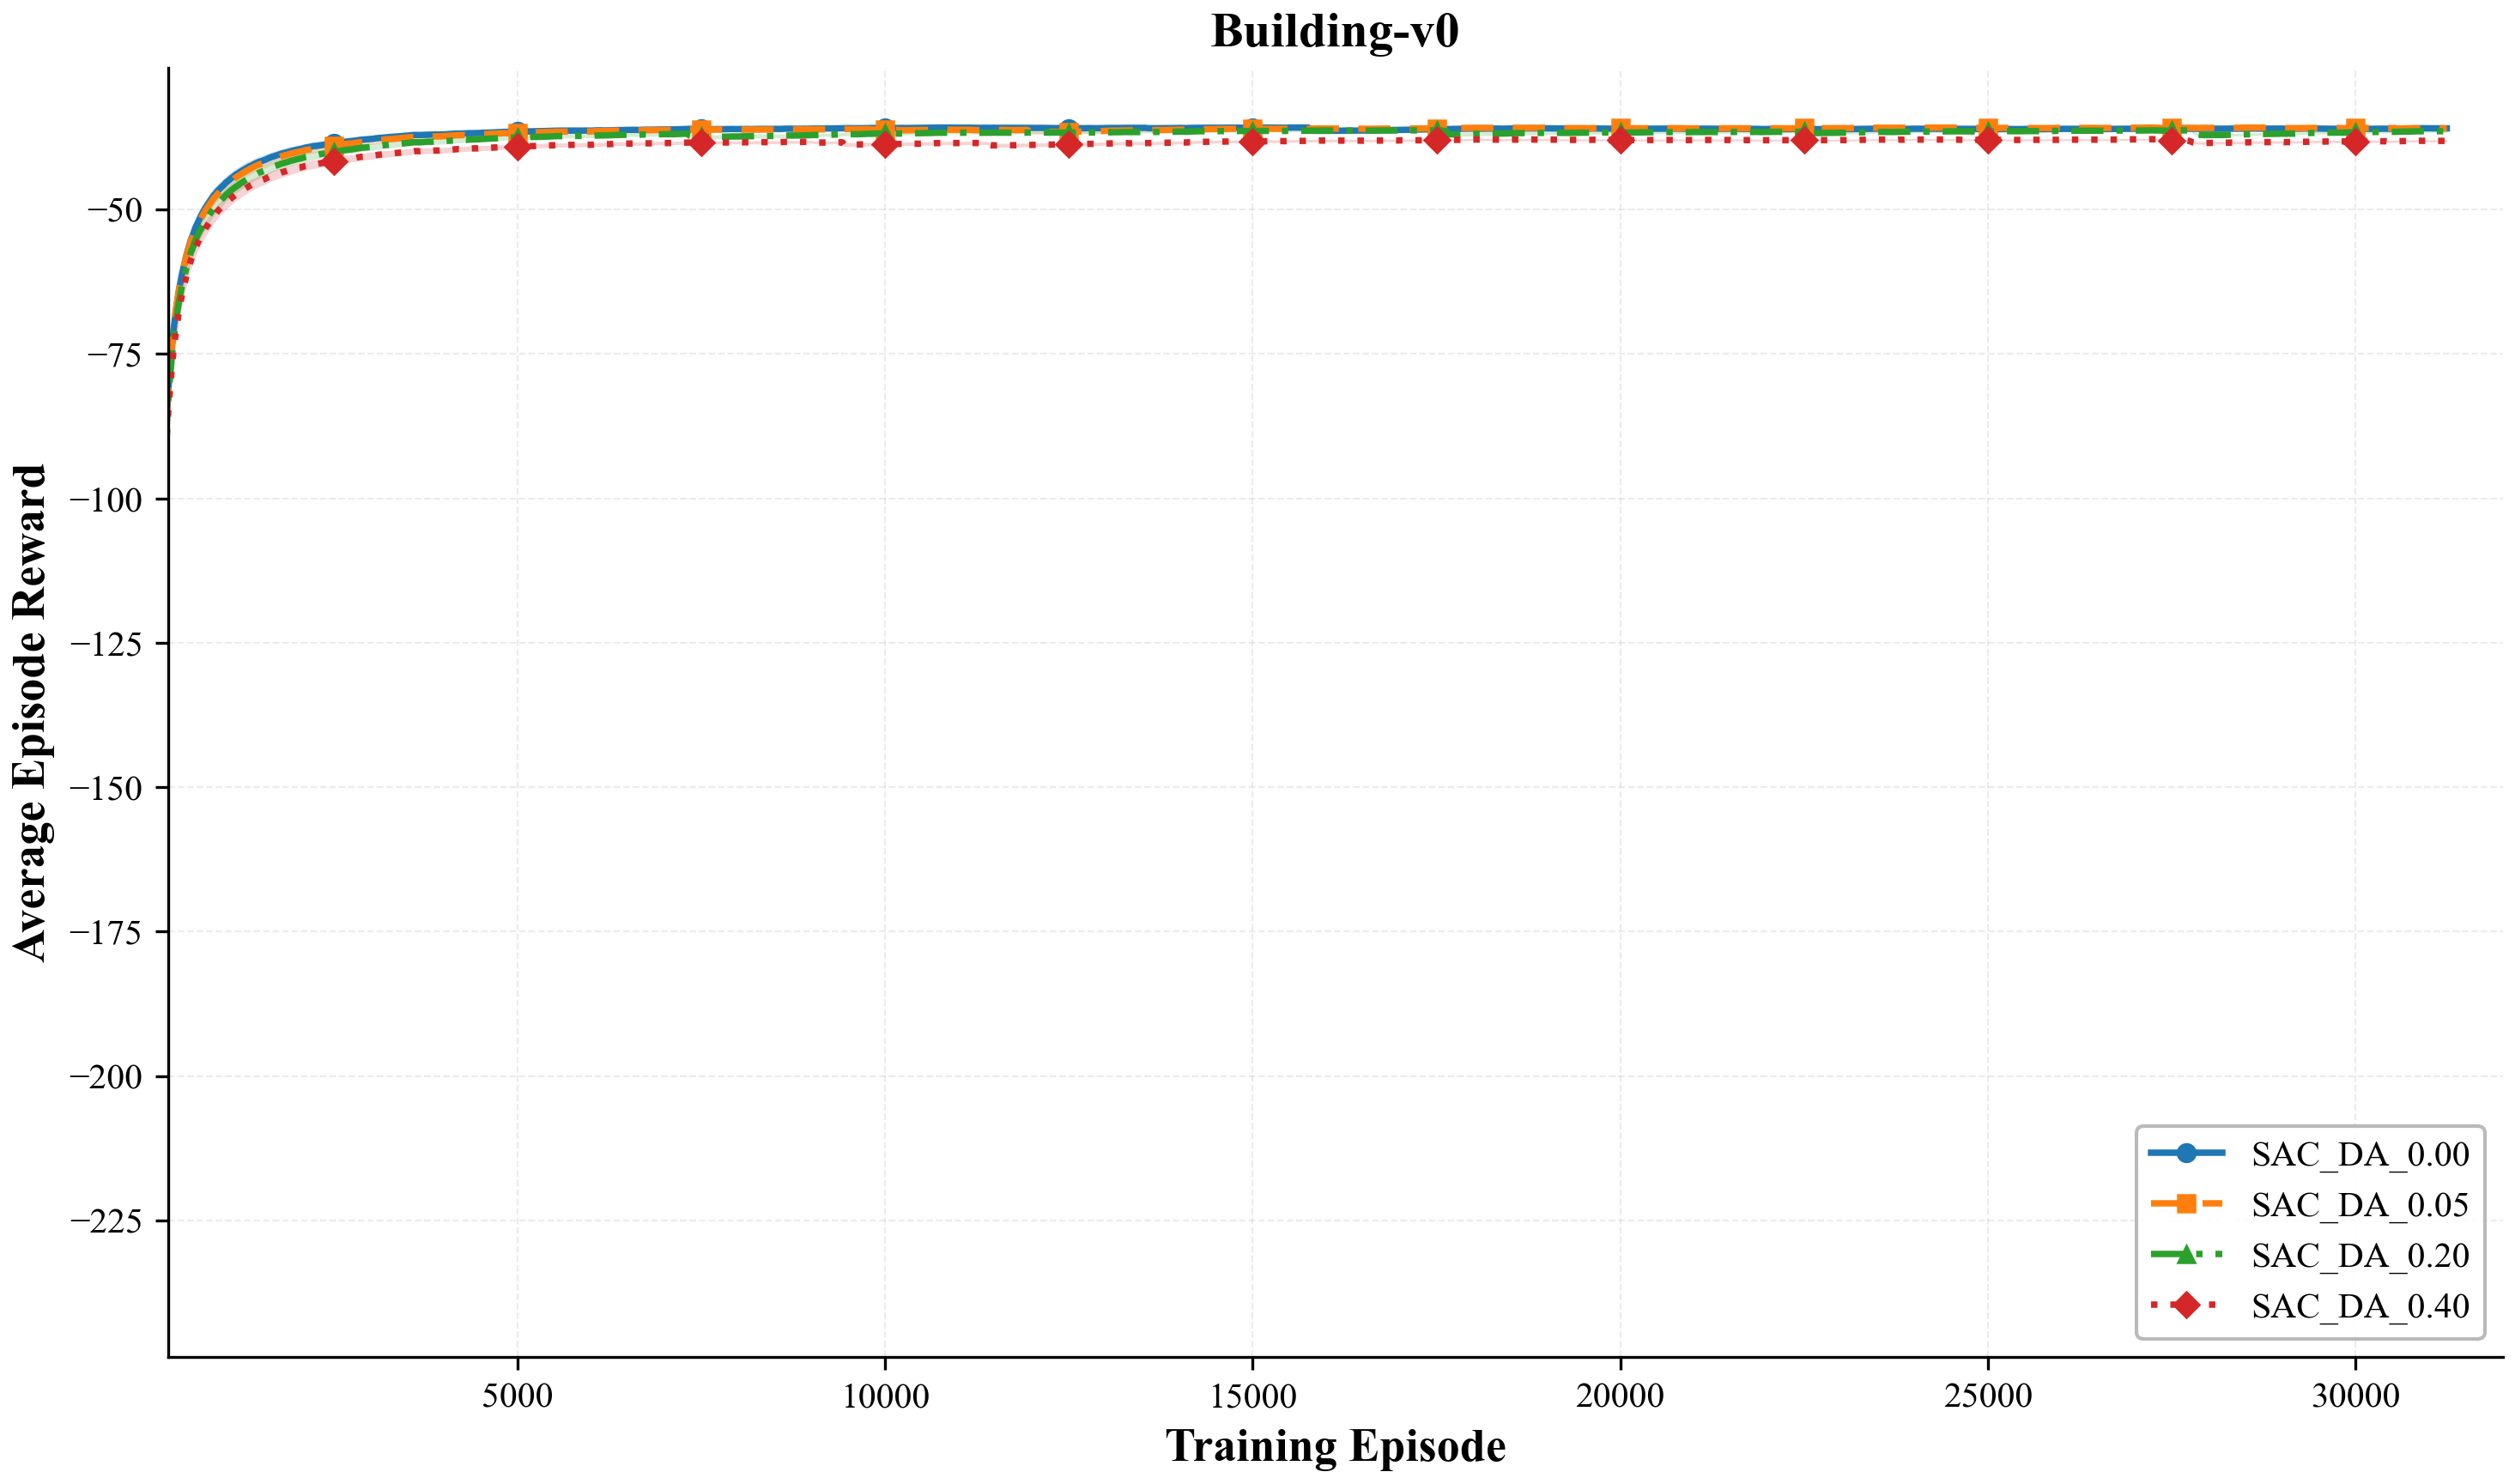
\includegraphics[width=0.9\textwidth]{figures/C_STDRL/bu/SAC/DA_2026-03-16_23-32-25.png}
\caption{Building SAC: Training curves under action noise (DA).}
\label{fig:stdrl_bu_sac_da}
\end{figure}

\begin{figure}[htbp]
\centering
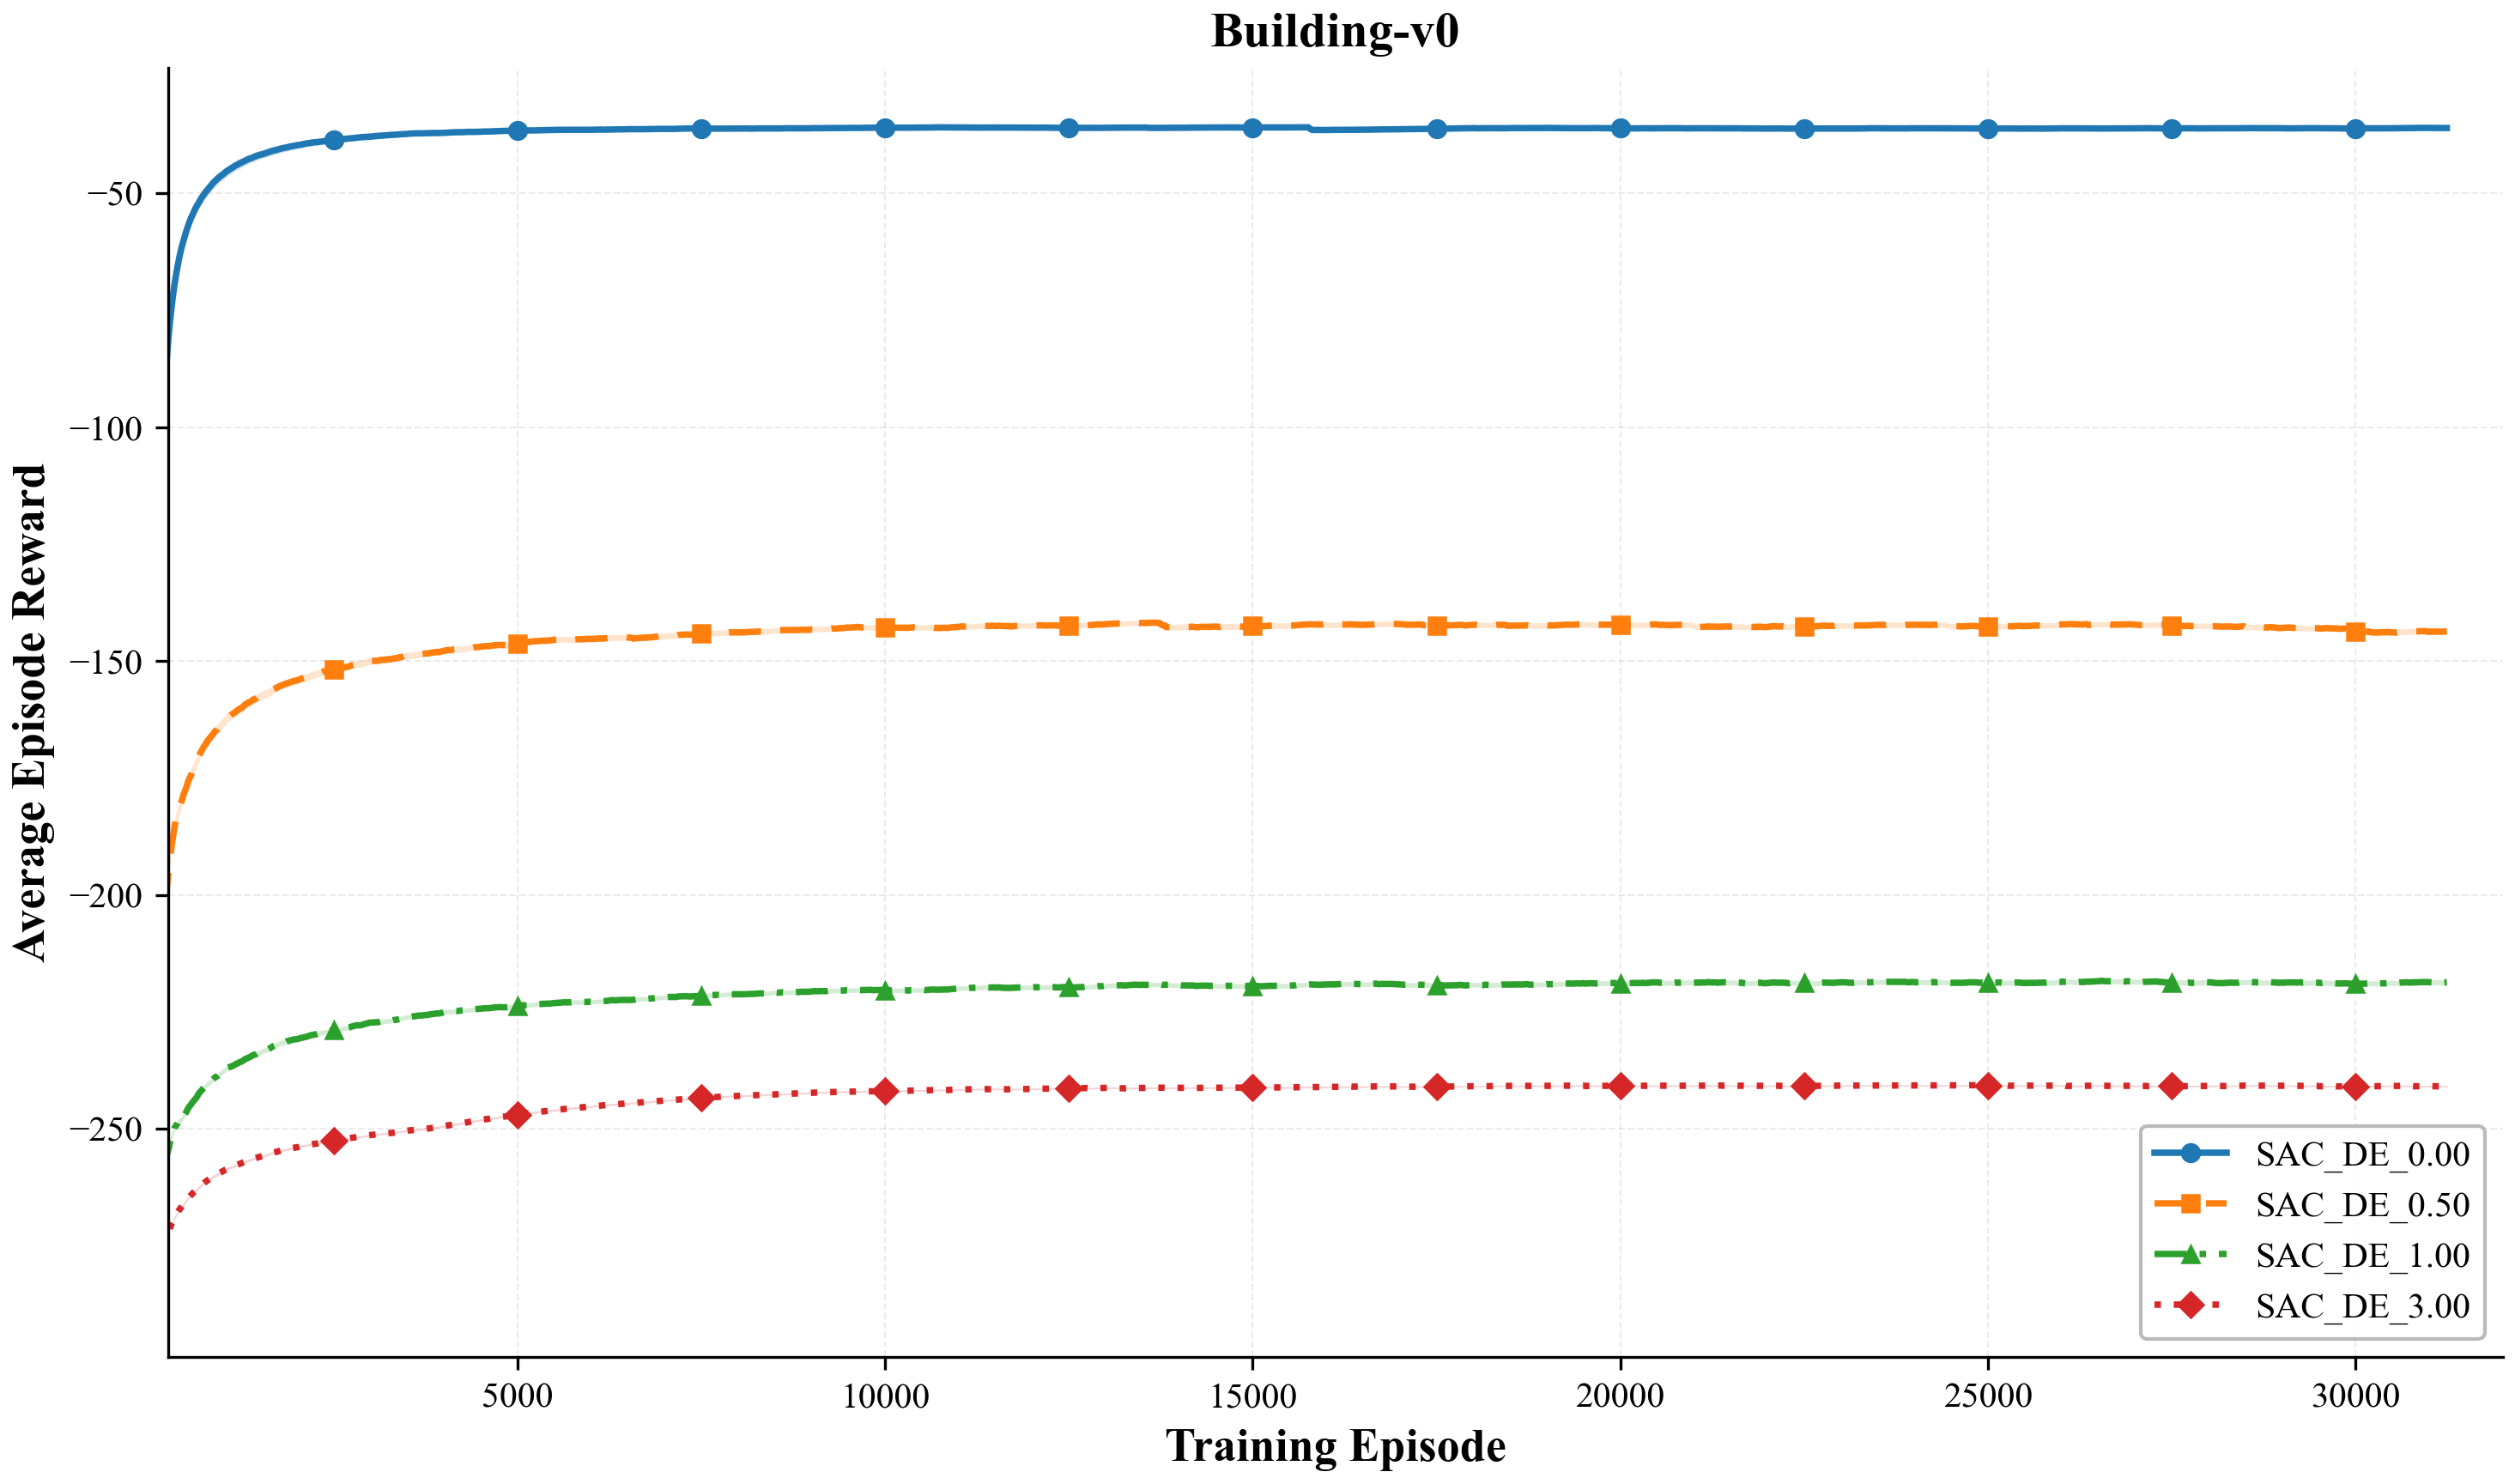
\includegraphics[width=0.9\textwidth]{figures/C_STDRL/bu/SAC/DE_2026-03-16_23-32-27.png}
\caption{Building SAC: Training curves under environment noise (DE).}
\label{fig:stdrl_bu_sac_de}
\end{figure}

\paragraph{Test-time robustness.} SAC's reward distributions (\Cref{fig:violin_bu_sac_obs,fig:violin_bu_sac_act,fig:violin_bu_sac_env}) show similar degradation patterns to PPO, confirming that the Building environment's noise sensitivity is environment-driven rather than algorithm-specific.

\begin{figure}[htbp]
\centering

\includegraphics[width=0.9\textwidth]{figures/C_POST/building/SAC/obs_violin.png}
\caption{Building SAC: Reward distribution under observation noise.}
\label{fig:violin_bu_sac_obs}
\end{figure}

\begin{figure}[htbp]
\centering

\includegraphics[width=0.9\textwidth]{figures/C_POST/building/SAC/action_violin.png}
\caption{Building SAC: Reward distribution under action noise.}
\label{fig:violin_bu_sac_act}
\end{figure}

\begin{figure}[htbp]
\centering

\includegraphics[width=0.9\textwidth]{figures/C_POST/building/SAC/env_violin.png}
\caption{Building SAC: Reward distribution under environment noise.}
\label{fig:violin_bu_sac_env}
\end{figure}

\begin{figure}[htbp]
\centering

\includegraphics[width=0.9\textwidth]{figures/C_POST/building/SAC/panel.png}
\caption{Building SAC: Summary panel across all three noise channels.}
\label{fig:post_bu_sac_panel}
\end{figure}

% ============================================================
\subsection{Cogeneration: Noise Robustness}
\label{sec:noise_co}

The Cogeneration environment reveals a striking algorithm-dependent divergence under noise: PPO is virtually immune to all noise types, while SAC degrades catastrophically under observation noise. This reflects fundamental differences in policy conservatism.

% --- Cogen PPO ---
\subsubsection{Cogeneration --- PPO}

\paragraph{Training curves.} PPO training curves (\Cref{fig:stdrl_co_ppo_ds,fig:stdrl_co_ppo_da,fig:stdrl_co_ppo_de}) are indistinguishable across noise levels, reflecting the conservative fuel-minimizing strategy that inherently tolerates perturbations.

\begin{figure}[htbp]
\centering
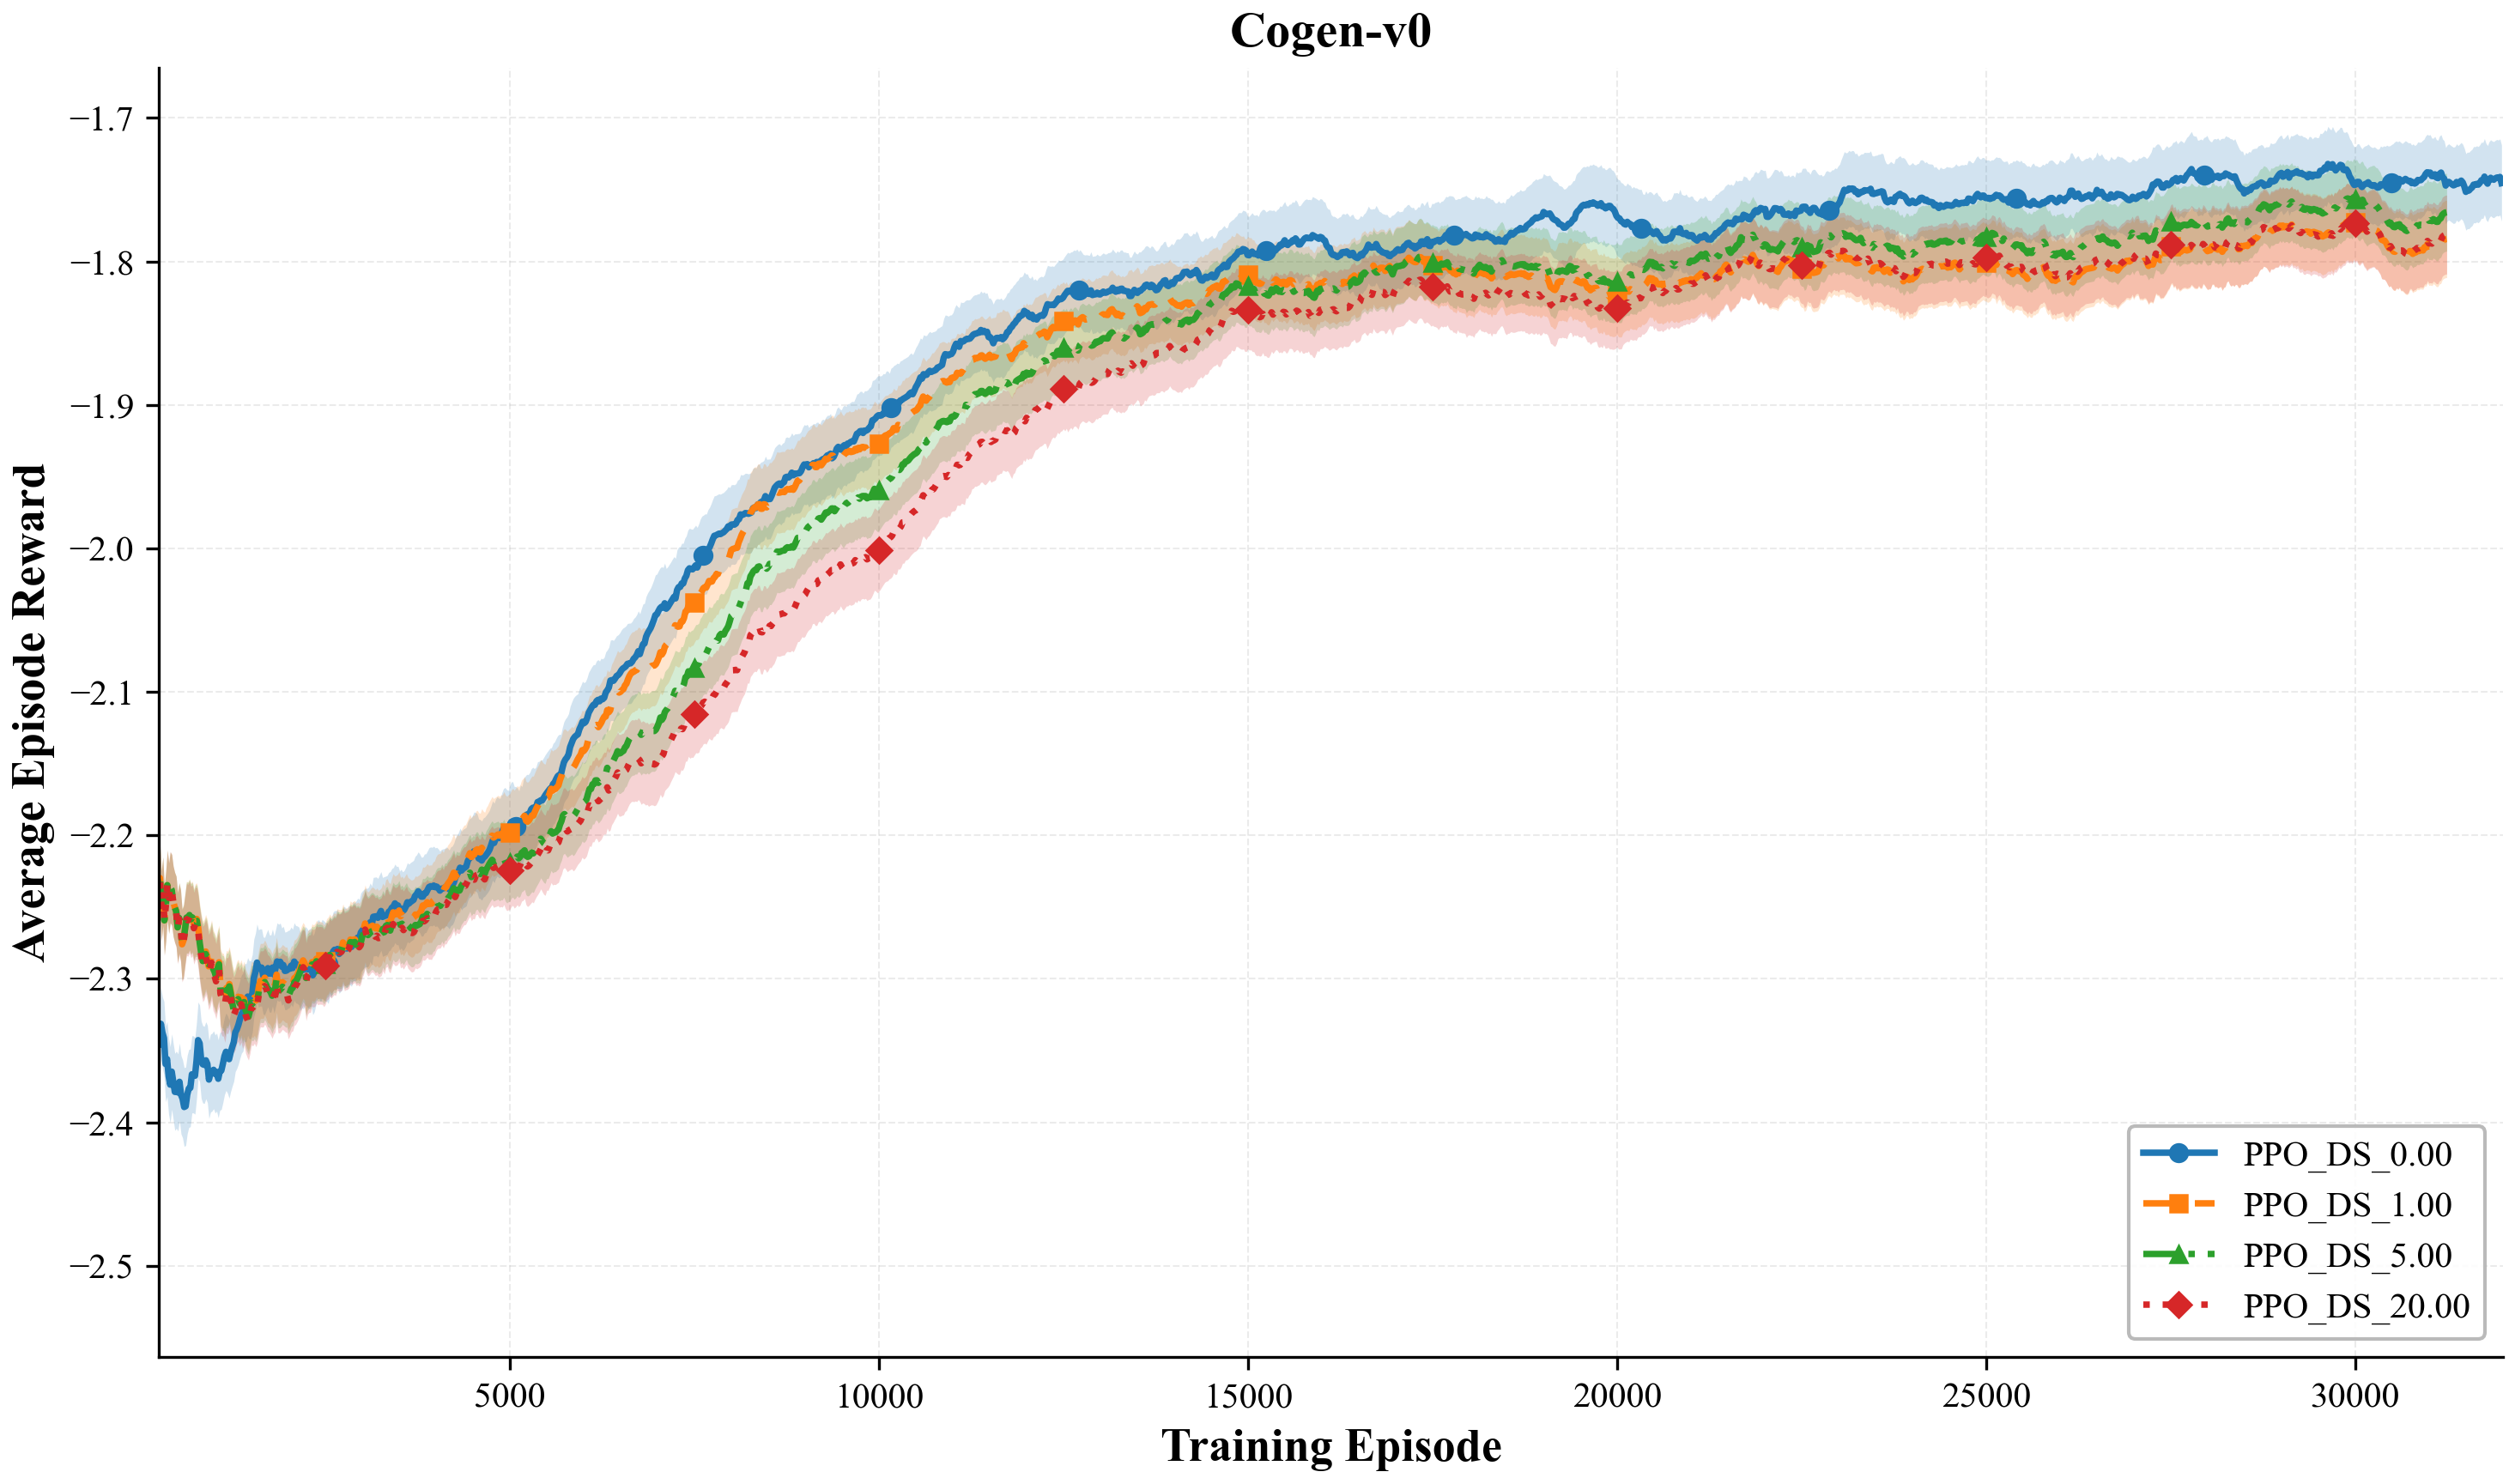
\includegraphics[width=0.9\textwidth]{figures/C_STDRL/co/PPO/DS_2026-03-16_23-32-34.png}
\caption{Cogen PPO: Training curves under observation noise (DS).}
\label{fig:stdrl_co_ppo_ds}
\end{figure}

\begin{figure}[htbp]
\centering
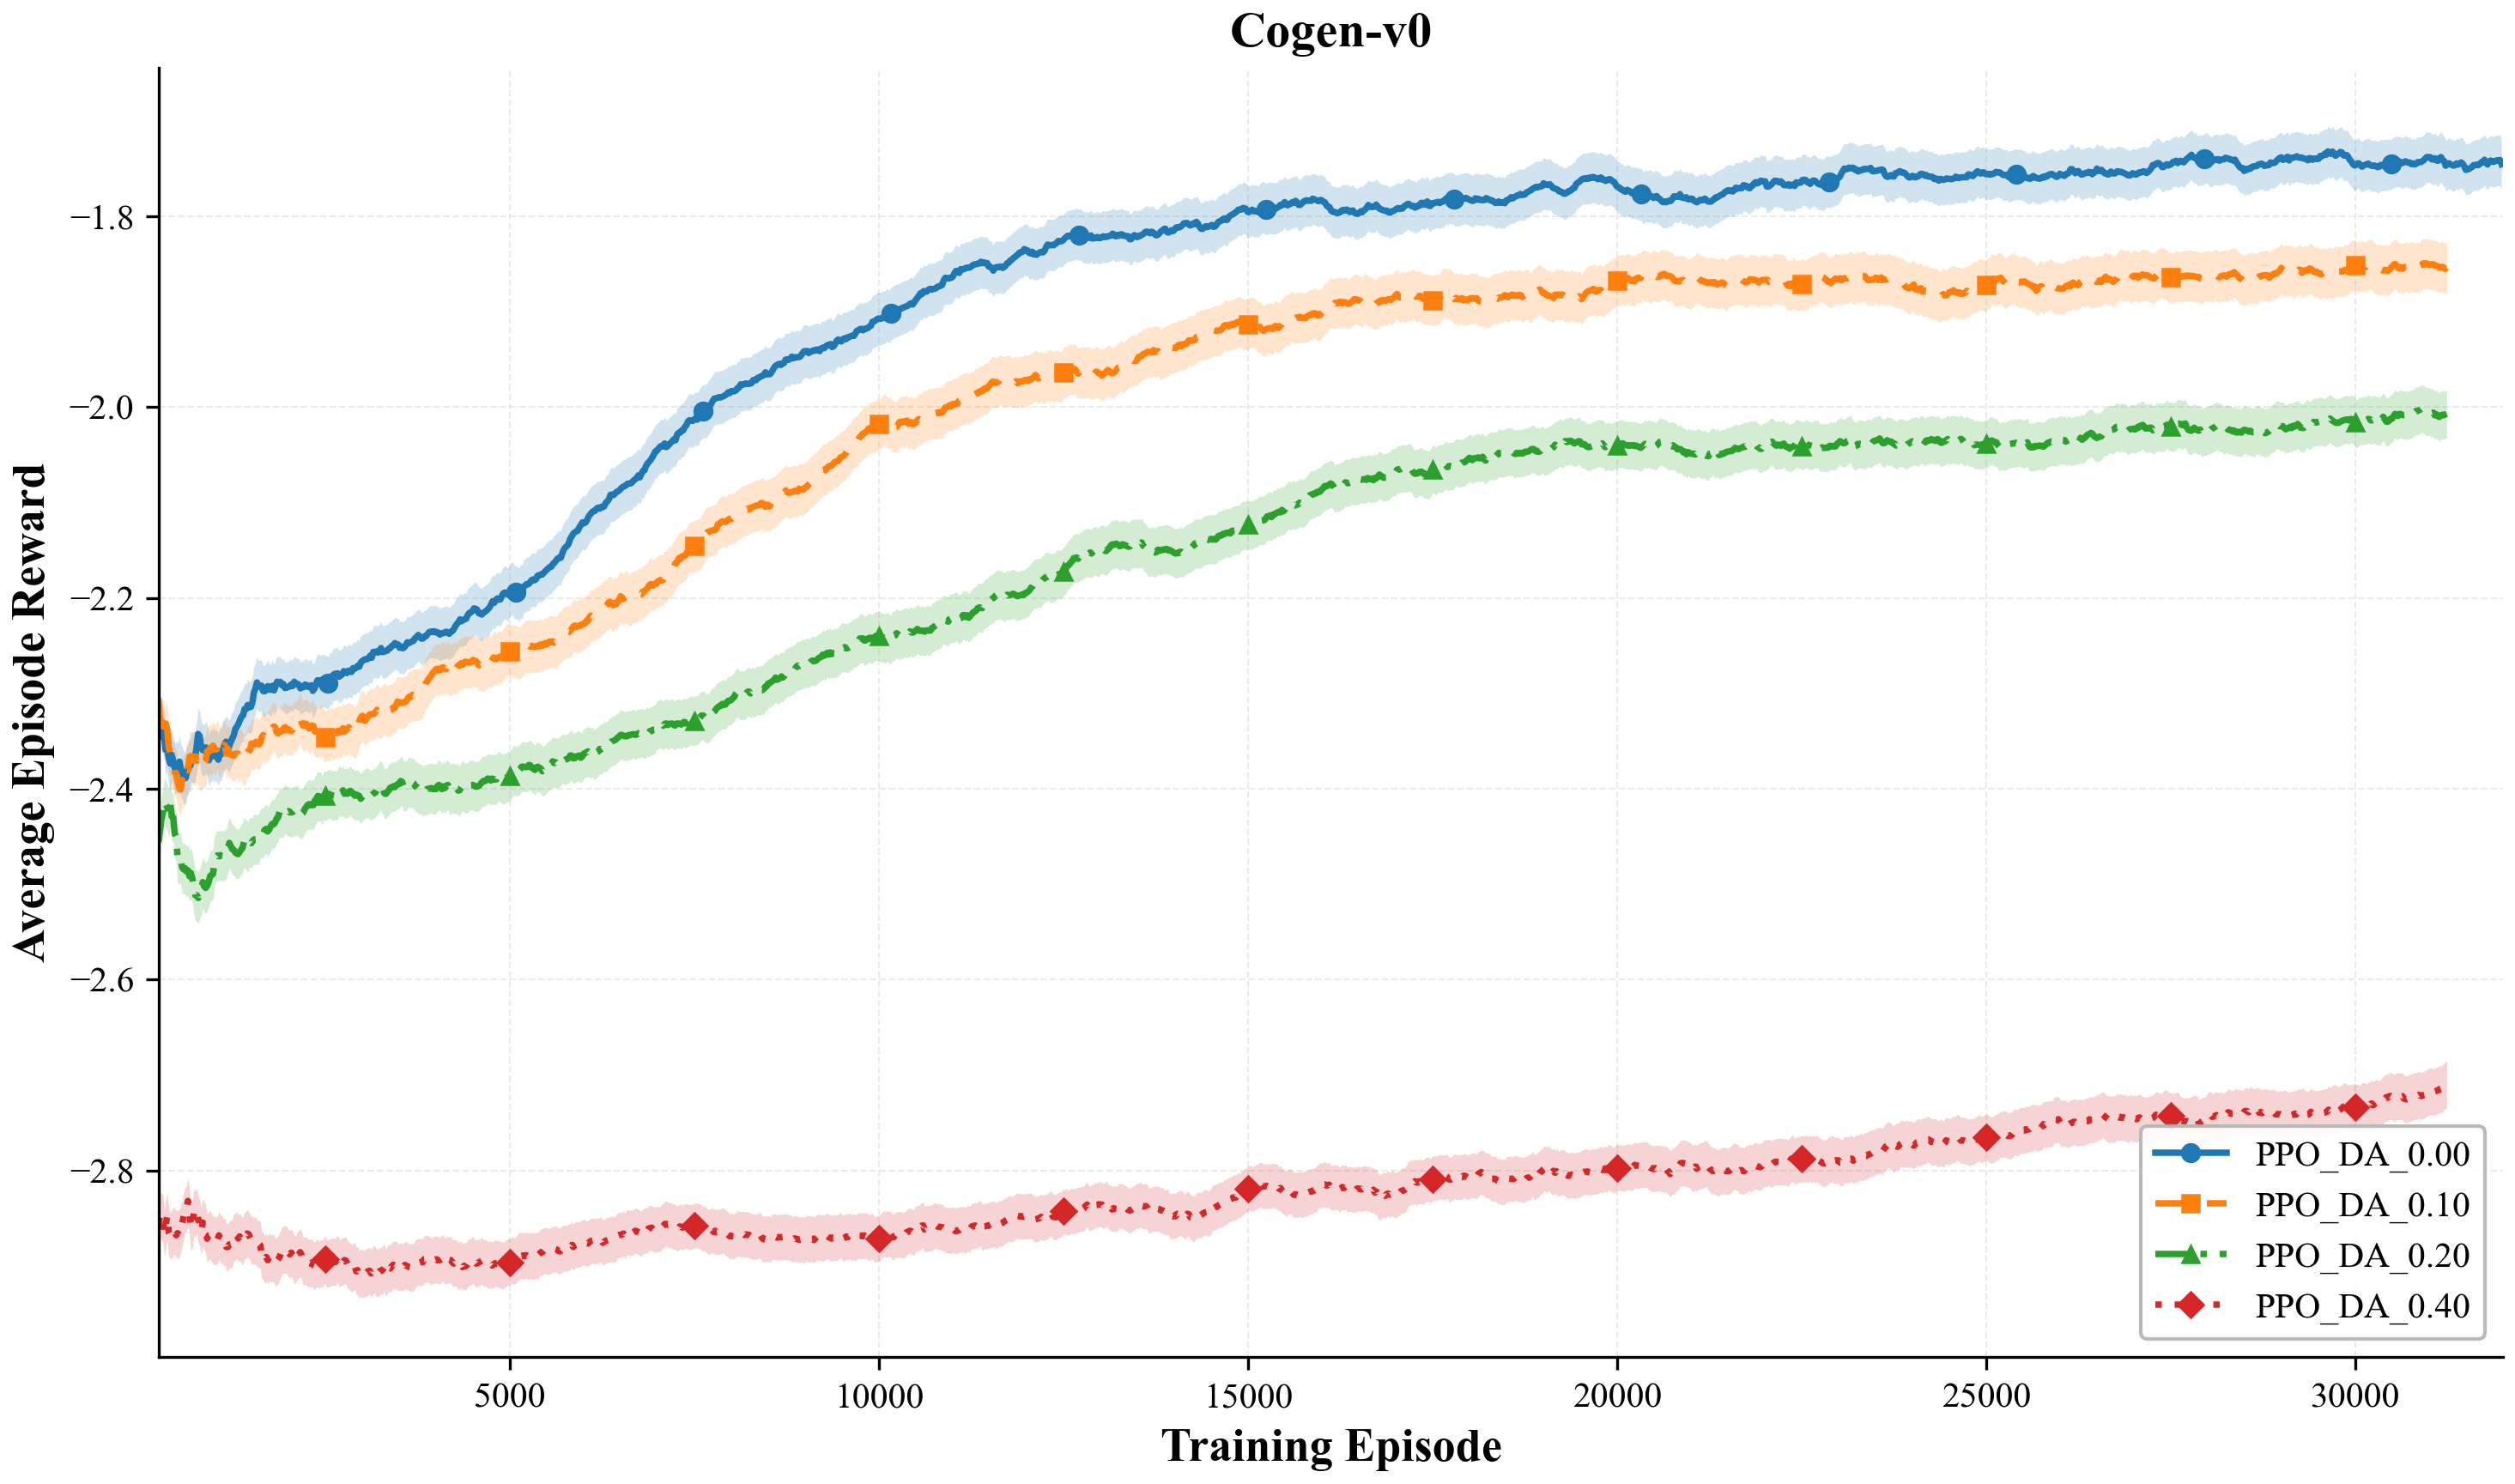
\includegraphics[width=0.9\textwidth]{figures/C_STDRL/co/PPO/DA_2026-03-16_23-32-36.png}
\caption{Cogen PPO: Training curves under action noise (DA).}
\label{fig:stdrl_co_ppo_da}
\end{figure}

\begin{figure}[htbp]
\centering
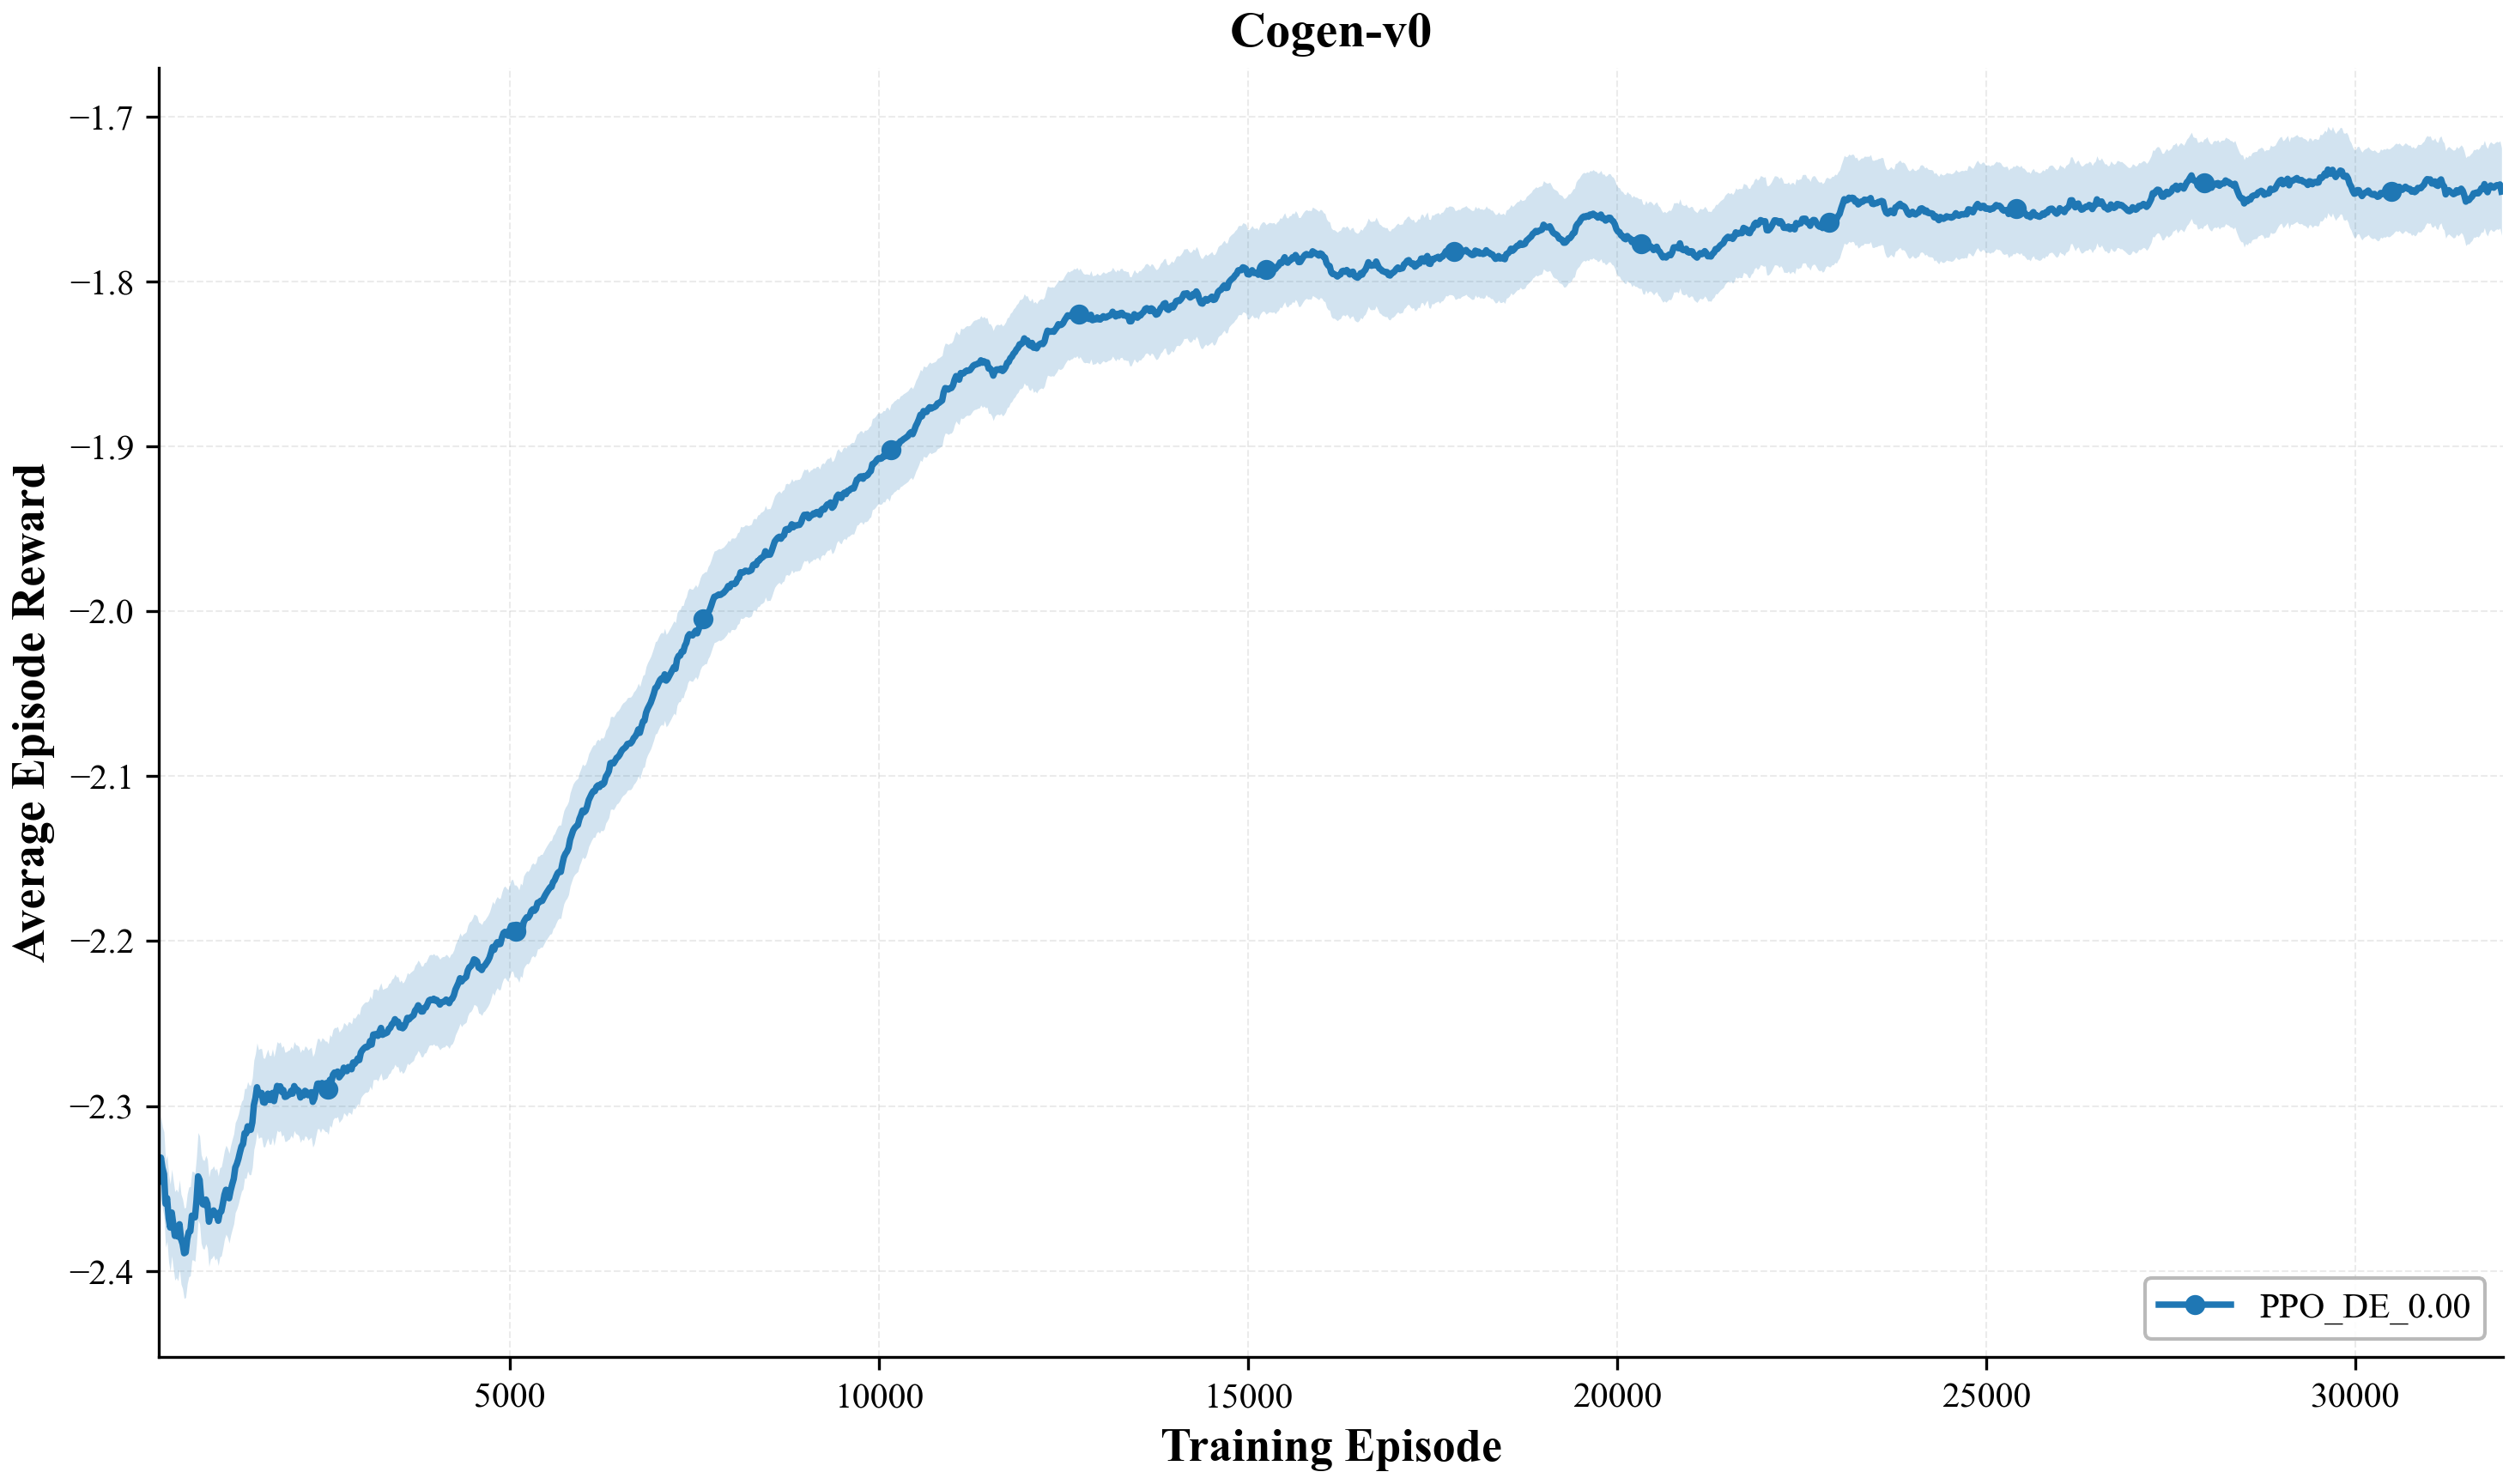
\includegraphics[width=0.9\textwidth]{figures/C_STDRL/co/PPO/DE_2026-03-16_23-32-38.png}
\caption{Cogen PPO: Training curves under environment noise (DE).}
\label{fig:stdrl_co_ppo_de}
\end{figure}

\paragraph{Test-time robustness.} The violin plots (\Cref{fig:violin_co_ppo_obs,fig:violin_co_ppo_act,fig:violin_co_ppo_env}) confirm that PPO's tight reward distribution remains virtually unchanged across the full noise range ($\sigma = 0$ to $5$). Less than $0.3\%$ degradation is observed across all noise channels, reflecting the conservative fuel-minimizing strategy where small actions are inherently insensitive to input perturbations.

\begin{figure}[htbp]
\centering

\includegraphics[width=0.9\textwidth]{figures/C_POST/cogen/PPO/obs_violin.png}
\caption{Cogen PPO: Reward distribution under observation noise. The tight distribution remains unchanged across the full noise range ($\sigma = 0$ to $5$).}
\label{fig:violin_co_ppo_obs}
\end{figure}

\begin{figure}[htbp]
\centering

\includegraphics[width=0.9\textwidth]{figures/C_POST/cogen/PPO/action_violin.png}
\caption{Cogen PPO: Reward distribution under action noise.}
\label{fig:violin_co_ppo_act}
\end{figure}

\begin{figure}[htbp]
\centering

\includegraphics[width=0.9\textwidth]{figures/C_POST/cogen/PPO/env_violin.png}
\caption{Cogen PPO: Reward distribution under environment noise.}
\label{fig:violin_co_ppo_env}
\end{figure}

\begin{figure}[htbp]
\centering

\includegraphics[width=0.9\textwidth]{figures/C_POST/cogen/PPO/panel.png}
\caption{Cogen PPO: Summary panel. Near-zero sensitivity across all noise channels.}
\label{fig:post_co_ppo_panel}
\end{figure}

% --- Cogen SAC ---
\subsubsection{Cogeneration --- SAC}

\paragraph{Training curves.} SAC training curves (\Cref{fig:stdrl_co_sac_ds,fig:stdrl_co_sac_da,fig:stdrl_co_sac_de}) show clear noise sensitivity, particularly under observation noise where convergence is disrupted at higher noise levels.

\begin{figure}[htbp]
\centering
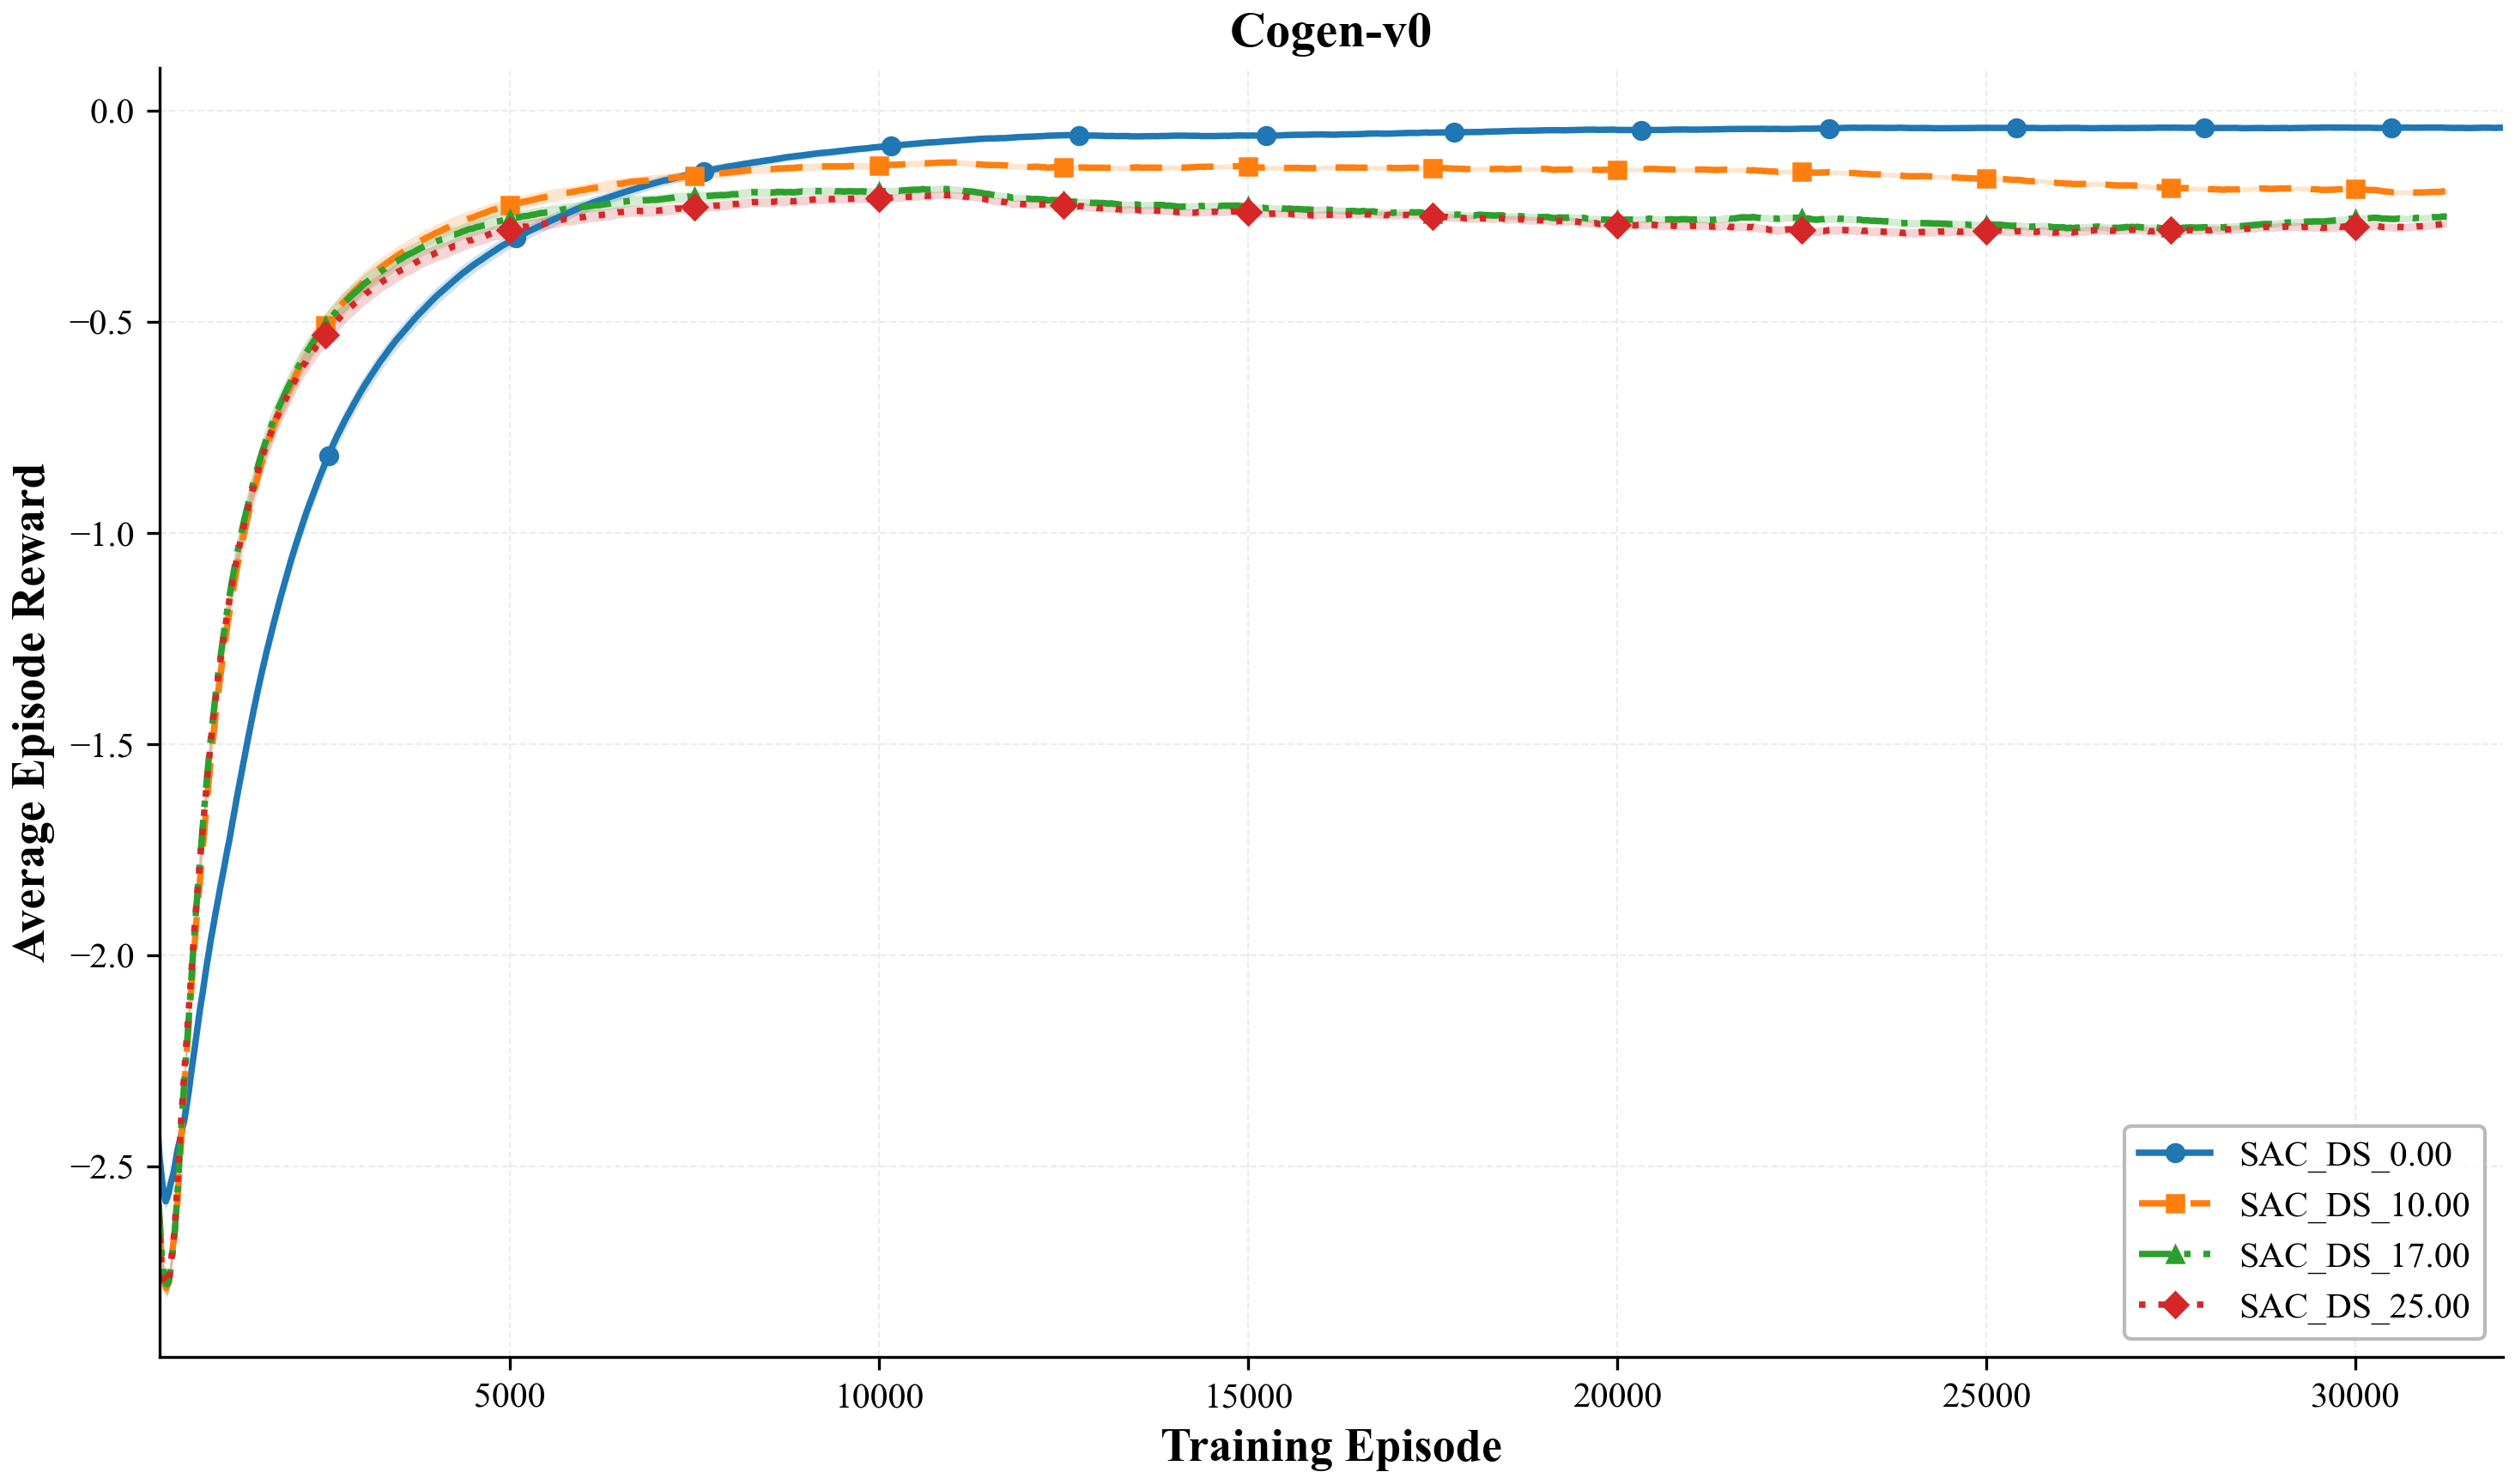
\includegraphics[width=0.9\textwidth]{figures/C_STDRL/co/SAC/DS_2026-03-16_23-32-40.png}
\caption{Cogen SAC: Training curves under observation noise (DS).}
\label{fig:stdrl_co_sac_ds}
\end{figure}

\begin{figure}[htbp]
\centering
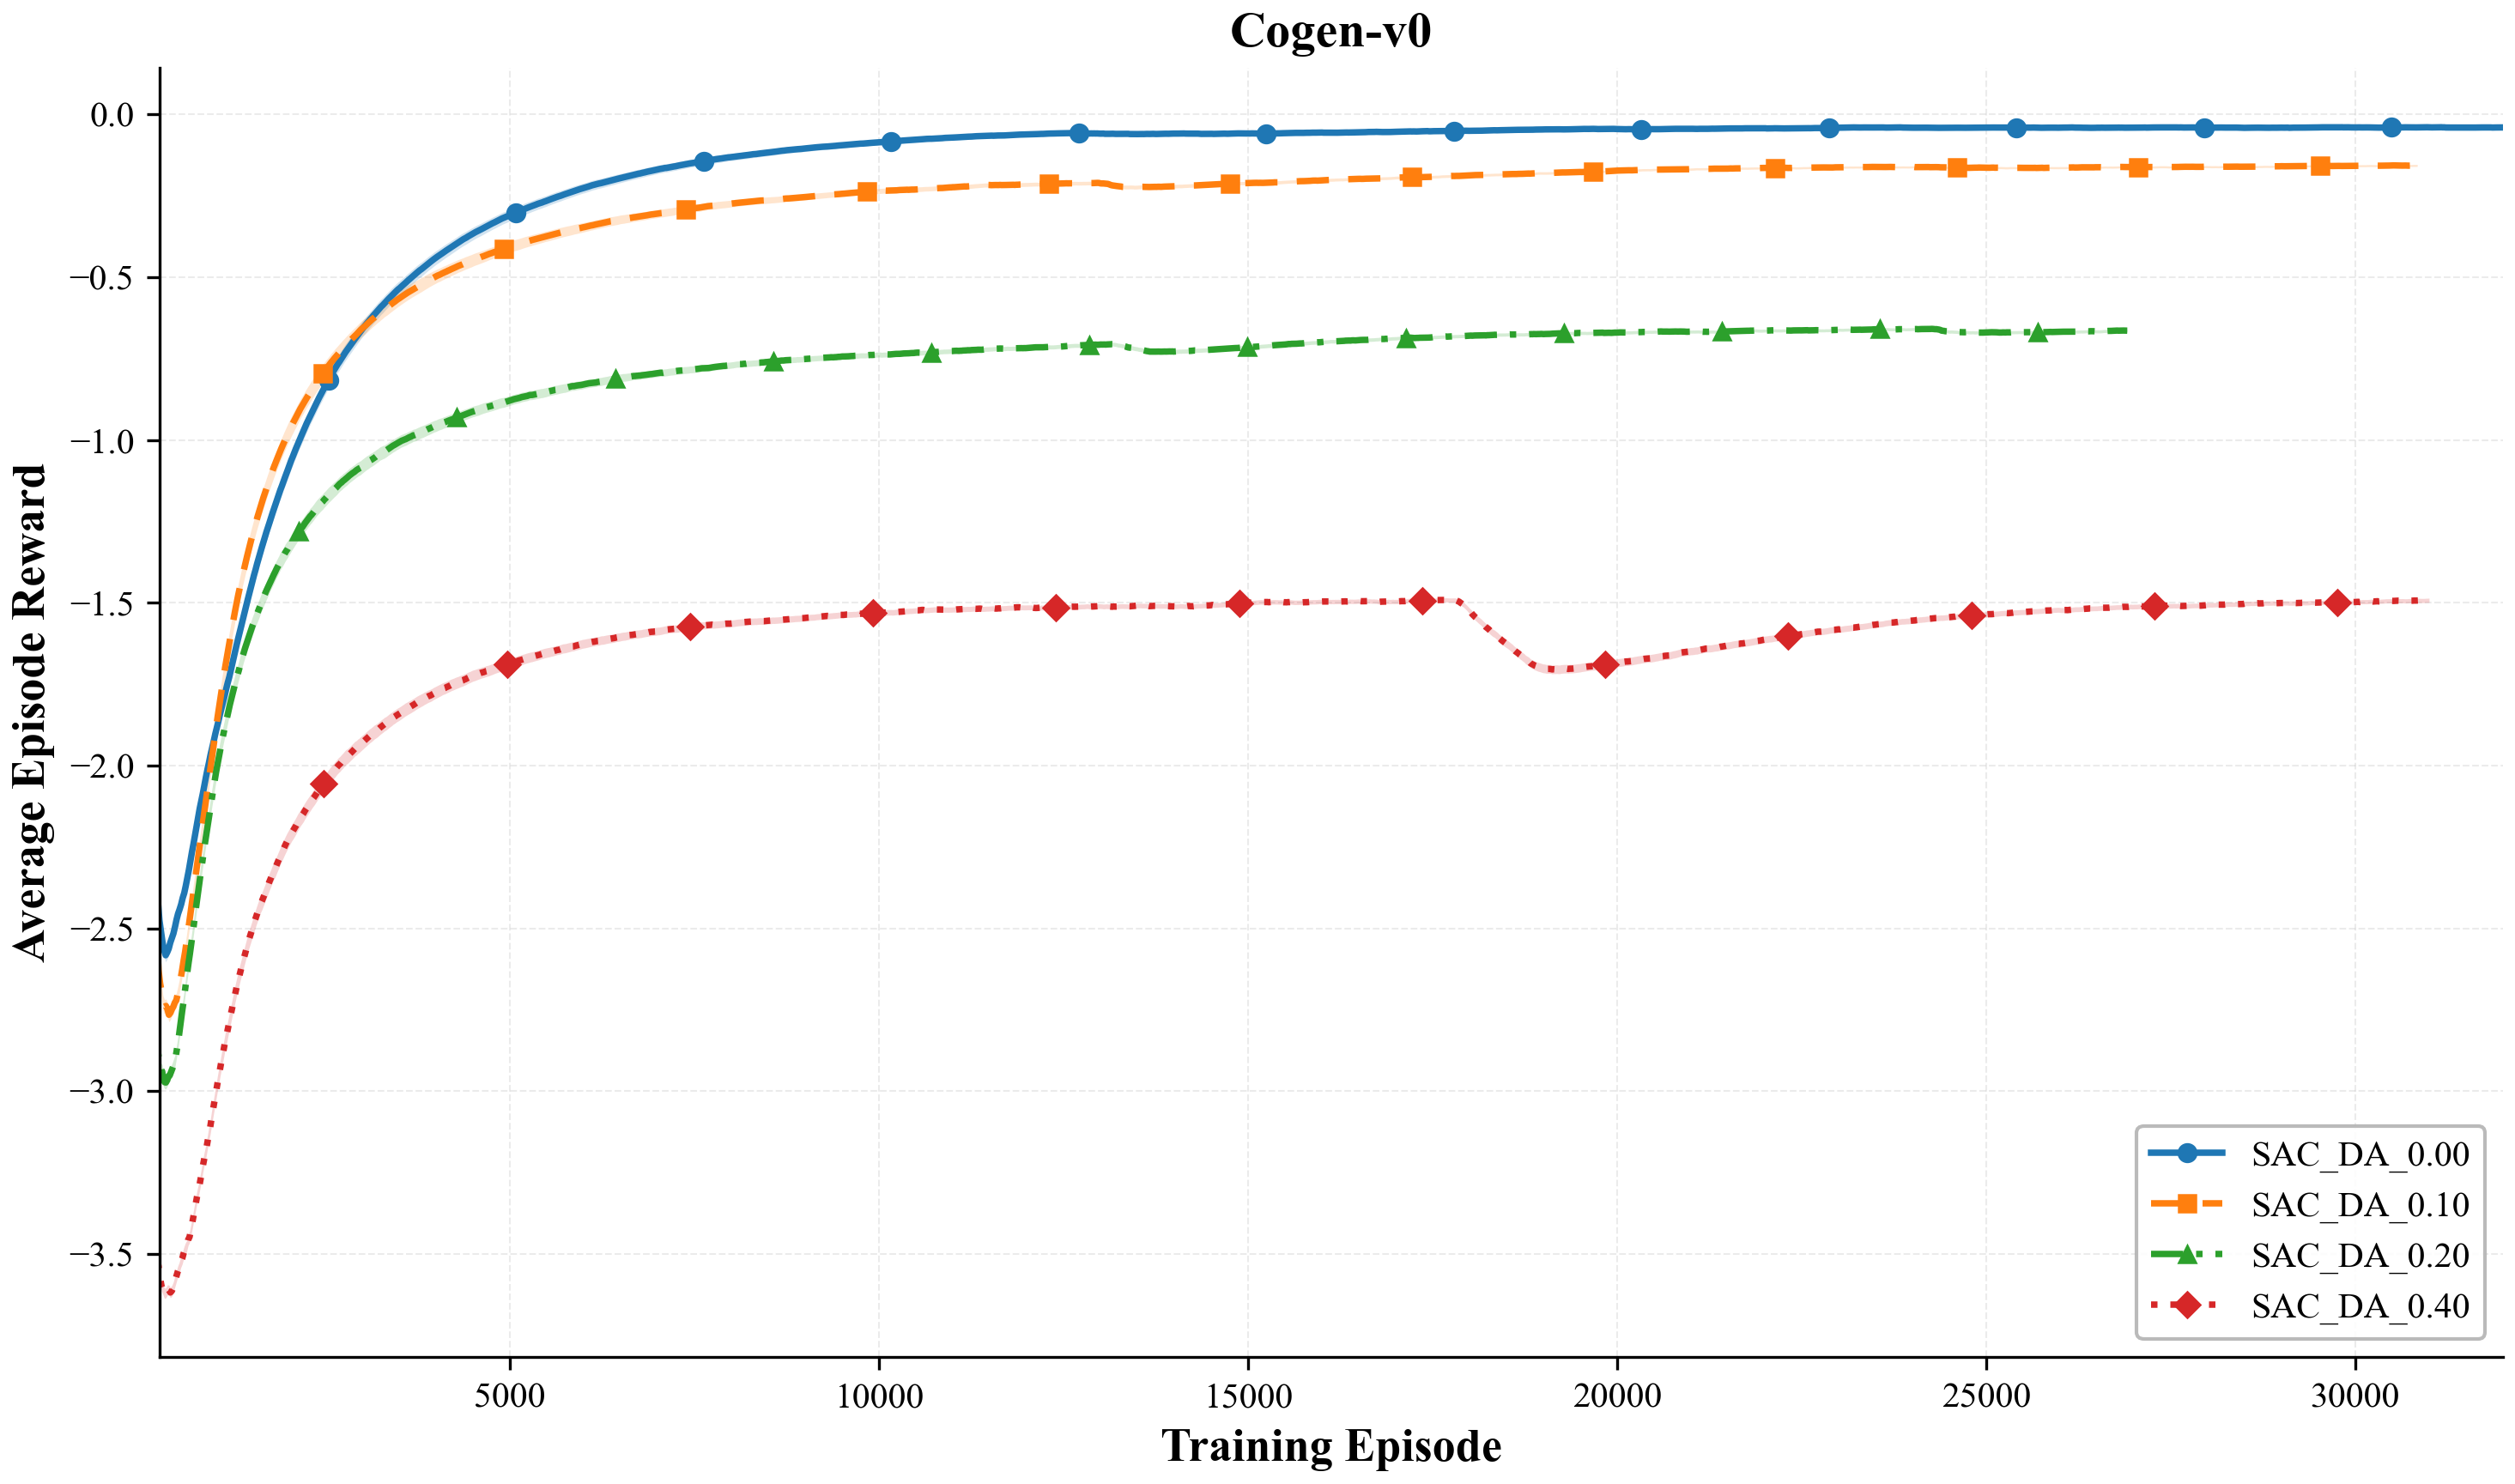
\includegraphics[width=0.9\textwidth]{figures/C_STDRL/co/SAC/DA_2026-03-16_23-32-42.png}
\caption{Cogen SAC: Training curves under action noise (DA).}
\label{fig:stdrl_co_sac_da}
\end{figure}

\begin{figure}[htbp]
\centering
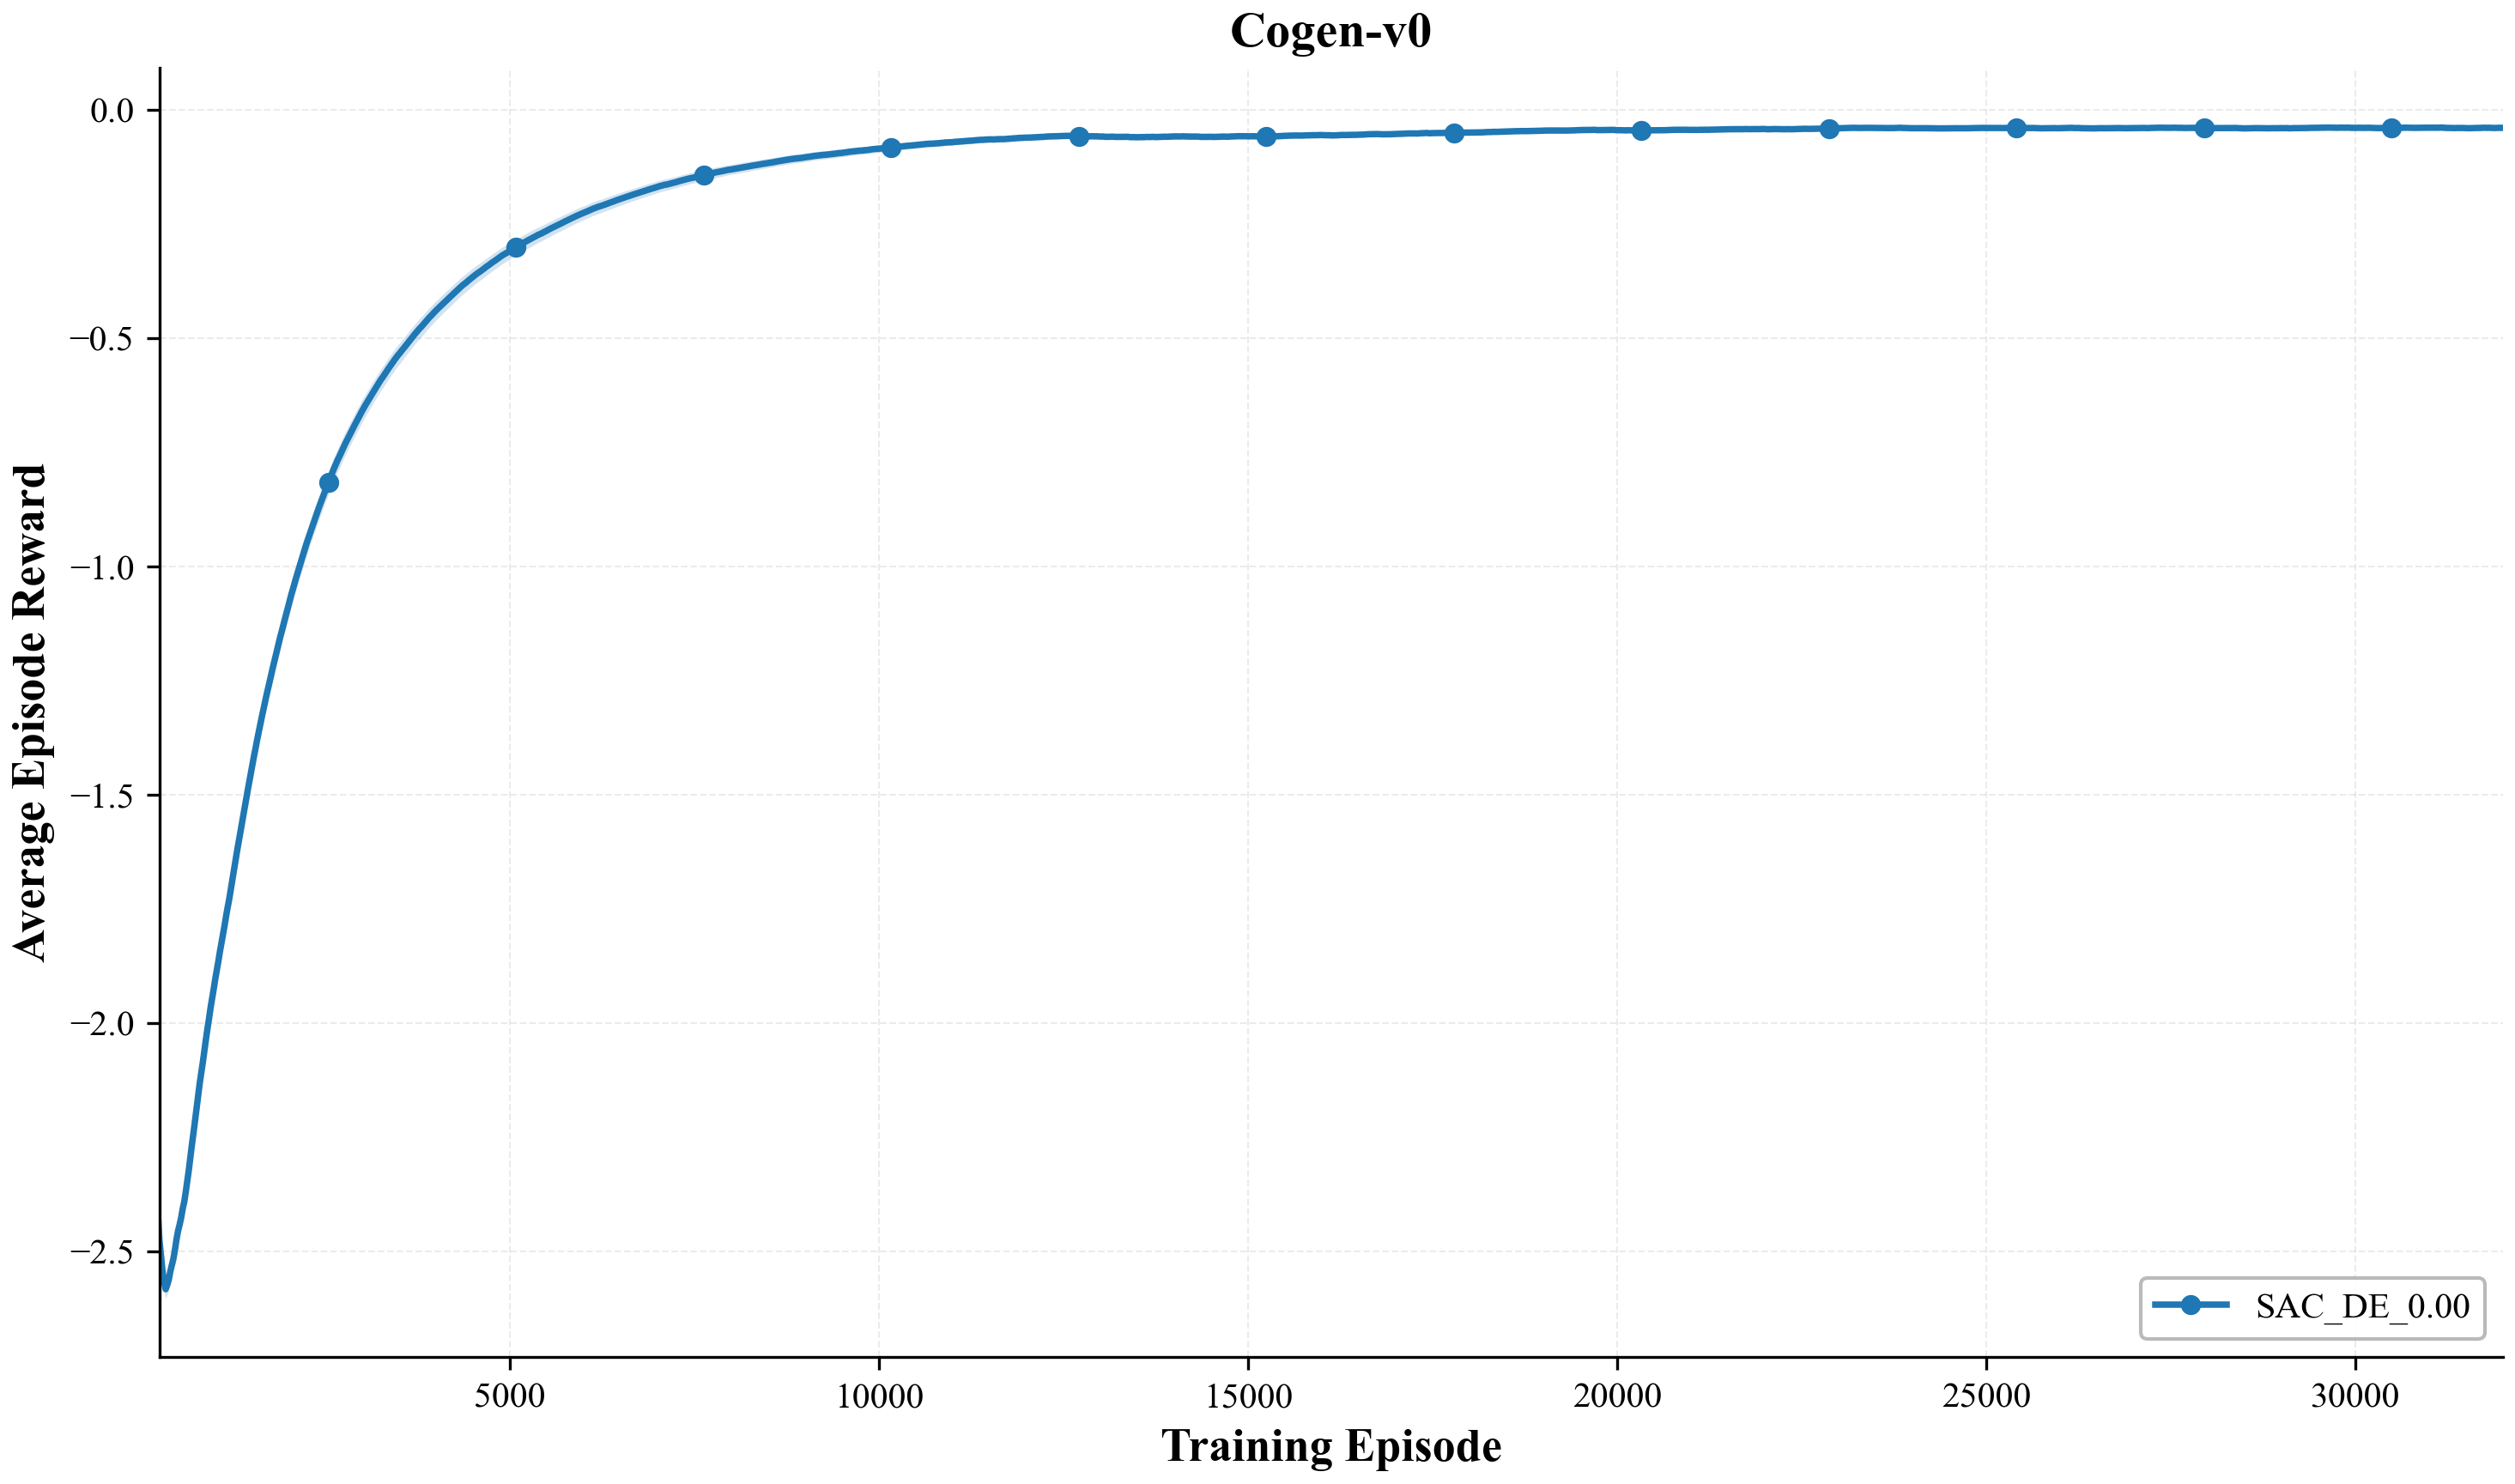
\includegraphics[width=0.9\textwidth]{figures/C_STDRL/co/SAC/DE_2026-03-16_23-32-44.png}
\caption{Cogen SAC: Training curves under environment noise (DE).}
\label{fig:stdrl_co_sac_de}
\end{figure}

\paragraph{Test-time robustness.} SAC's observation noise violin plot (\Cref{fig:violin_co_sac_obs}) shows dramatic degradation: the distribution broadens and shifts leftward, with heavy left tails emerging at $\sigma \geq 2$ indicating frequent constraint violations. SAC's aggressive optimization near the constraint boundary is fragile to observation perturbations. Environment noise (\Cref{fig:violin_co_sac_env}) causes moderate degradation through ONNX model output perturbations.

\begin{figure}[htbp]
\centering

\includegraphics[width=0.9\textwidth]{figures/C_POST/cogen/SAC/obs_violin.png}
\caption{Cogen SAC: Reward distribution under observation noise. Heavy left tails emerge at $\sigma \geq 2$, indicating constraint violations from aggressive near-boundary optimization.}
\label{fig:violin_co_sac_obs}
\end{figure}

\begin{figure}[htbp]
\centering

\includegraphics[width=0.9\textwidth]{figures/C_POST/cogen/SAC/env_violin.png}
\caption{Cogen SAC: Reward distribution under environment noise. ONNX model output perturbations cause moderate degradation with increasing tail weight.}
\label{fig:violin_co_sac_env}
\end{figure}

\begin{figure}[htbp]
\centering

\includegraphics[width=0.9\textwidth]{figures/C_POST/cogen/SAC/panel.png}
\caption{Cogen SAC: Summary panel. Observation noise causes severe degradation; environment noise has moderate impact.}
\label{fig:post_co_sac_panel}
\end{figure}

% ============================================================
\subsection{Noise Robustness Findings}
\label{sec:noise_findings}

\begin{finding}[Environment-Dependent Noise Sensitivity (RQ1, RQ6)]
\label{find:noise_sensitivity}
Noise robustness varies dramatically across environments: EV Charging policies are exceptionally robust to all noise types ($<1\%$ degradation at moderate noise), while Building policies degrade rapidly under observation and environment noise ($>100\%$ degradation at $\sigma \geq 0.15$). This reflects fundamental differences in environment dynamics: EV Charging's reward depends primarily on aggregate daily charging patterns that are noise-resistant, while Building's RC thermal model amplifies per-timestep observation errors through coupled zone dynamics.
\end{finding}

\begin{finding}[Observation vs.\ Action Noise Asymmetry (RQ2)]
\label{find:obs_act_asymmetry}
Across all environments, observation noise causes significantly more degradation than action noise at equivalent scales. The practical implication is clear: for real-world deployment of RL-based controllers, sensor accuracy is more critical than actuator precision.
\end{finding}

\begin{finding}[Algorithm-Specific Robustness (RQ1)]
\label{find:algo_robustness}
PPO consistently demonstrates superior noise robustness compared to SAC and TD3, with the most dramatic difference in Cogeneration (PPO: $<0.3\%$ degradation; SAC: $>2000\%$ degradation). PPO's on-policy training and clipped surrogate objective create naturally conservative policies that tolerate input perturbations, while SAC's entropy-maximizing exploration can amplify noise in the policy output.
\end{finding}

% ============================================================
\section{Safe Reinforcement Learning}
\label{sec:results_saferl}

We evaluate four on-policy CMDP algorithms---PPO-Lagrangian (PPOLag), CPO, OnCRPO, and FOCOPS---under varying cost limits using the CMDP formulations described in \Cref{sec:safe_rl}. All models are trained for 6M steps (3000 epochs $\times$ 2000 steps/epoch) using the OmniSafe framework~\citep{ji2023omnisafe} with the hyperparameters specified in \Cref{sec:experimental_design}.

% ------------------------------------------------------------
\subsection{Cogeneration: Strong Constraint Differentiation}
\label{sec:saferl_cogen}

The Cogeneration environment provides the strongest Safe RL results. The CMDP cost---cumulative turbine ramping stress---is orthogonal to the reward, which is dominated by fuel and delivery costs. The reward's built-in ramp penalty ($w_{\text{ramp}} = 2$) is negligible, so the unconstrained agent ignores turbine stress.

% --- Cogen PPOLag ---
\subsubsection{Cogeneration --- PPOLag}

PPOLag achieves the clearest cost limit differentiation (\Cref{fig:cogen_ppolag}): final episode costs of $5$, $12$, $23$, and $43$ for $d = 10, 25, 50, 200$ respectively---a monotonically increasing sequence. The tightest limit ($d=10$) incurs a reward penalty of $-0.30$ compared to $-0.04$ for loose limits, quantifying the economic cost of smooth turbine operation.

\begin{figure}[htbp]
\centering
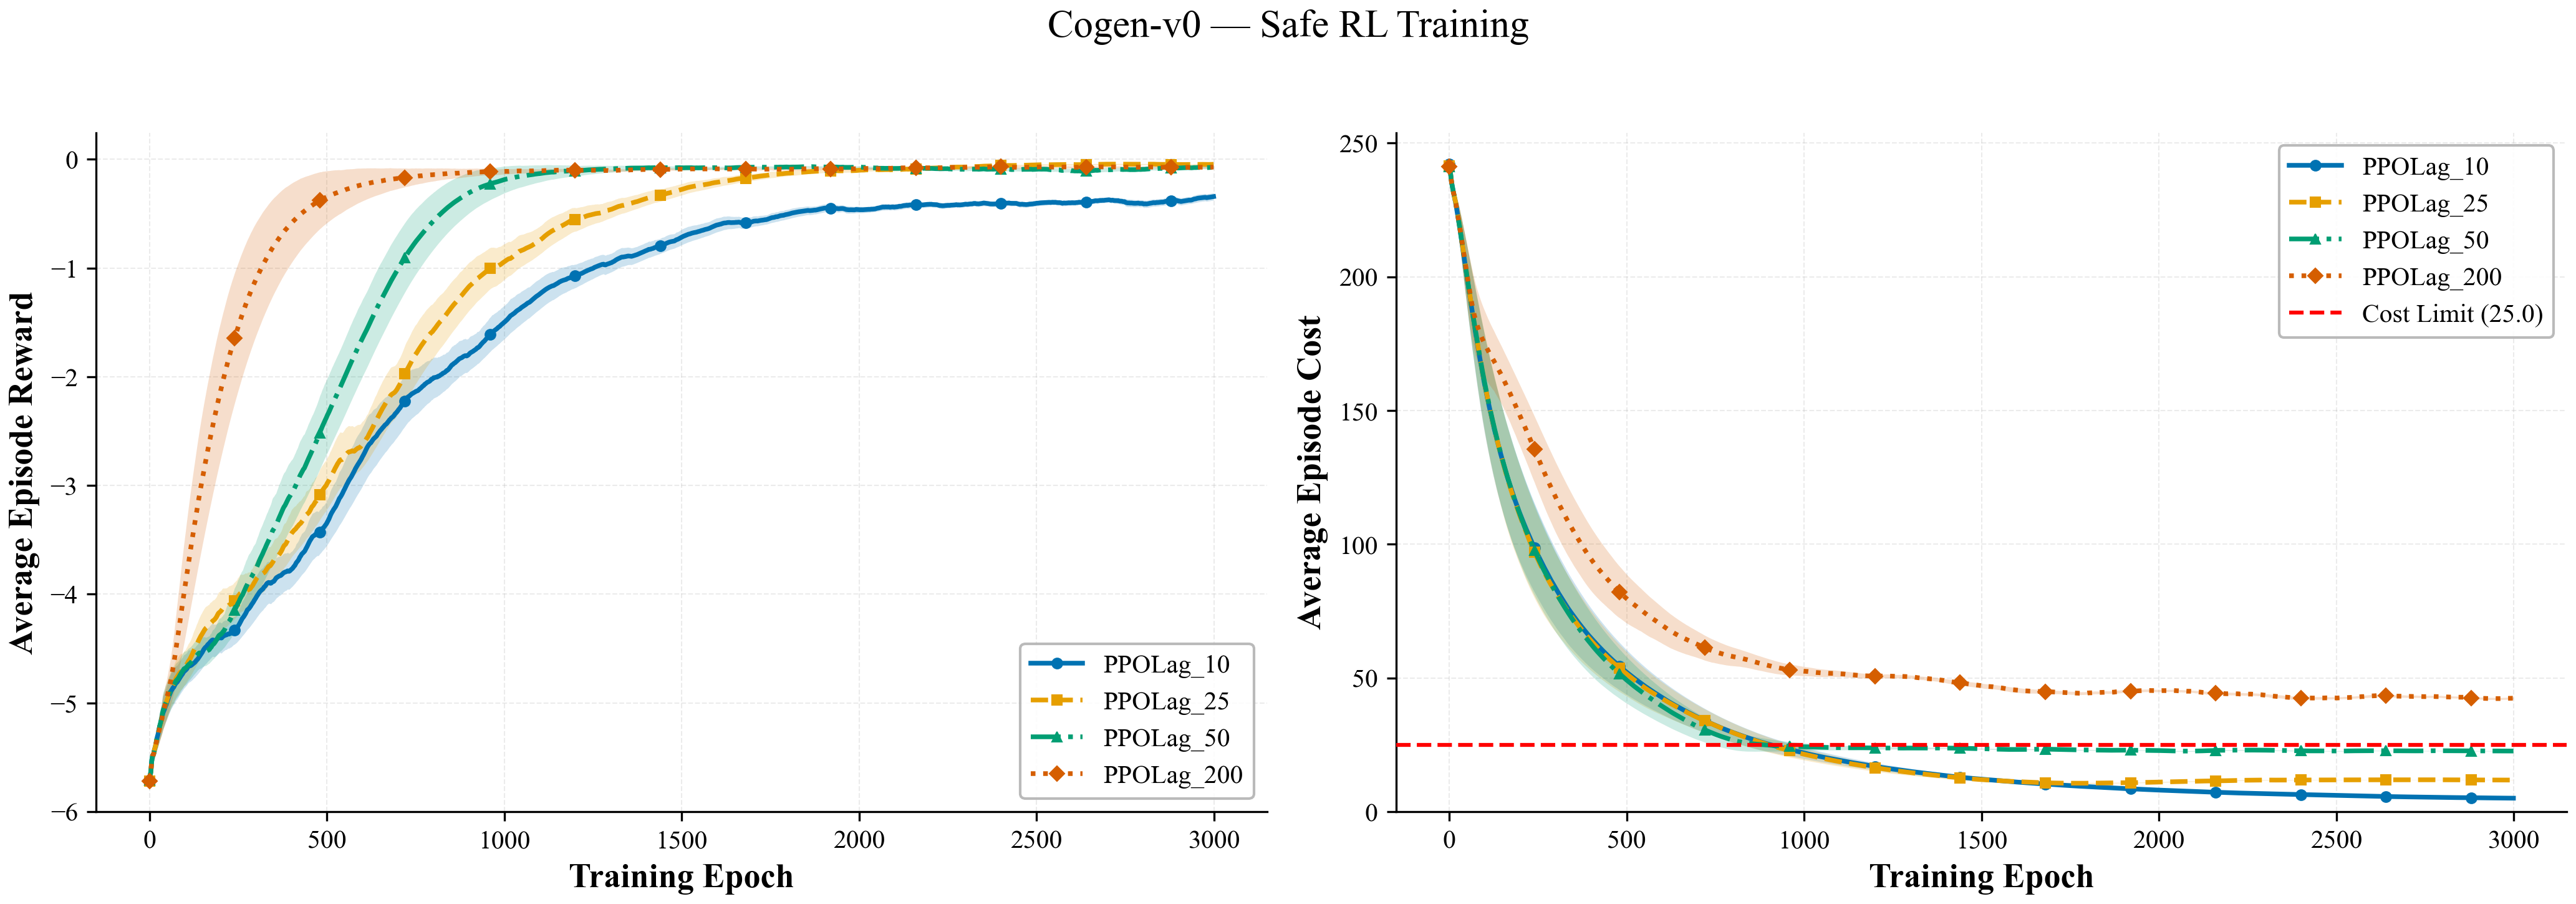
\includegraphics[width=0.9\textwidth]{figures/C_SRL/cogen/saferl_cogen_PPOLag_3000ep_200ema.png}
\caption{Cogen PPOLag: Dual-panel training curves (reward left, cost right) for cost limits $d \in \{10, 25, 50, 200\}$. Clear monotonic differentiation with dashed red line indicating $d = 25$ reference.}
\label{fig:cogen_ppolag}
\end{figure}

% --- Cogen CPO ---
\subsubsection{Cogeneration --- CPO}

CPO reduces cost rapidly ($\sim$500 epochs) but exhibits weaker limit differentiation than PPOLag (\Cref{fig:srl_co_cpo}). The trust-region update converges quickly but lacks the fine-grained control of Lagrangian relaxation.

\begin{figure}[htbp]
\centering
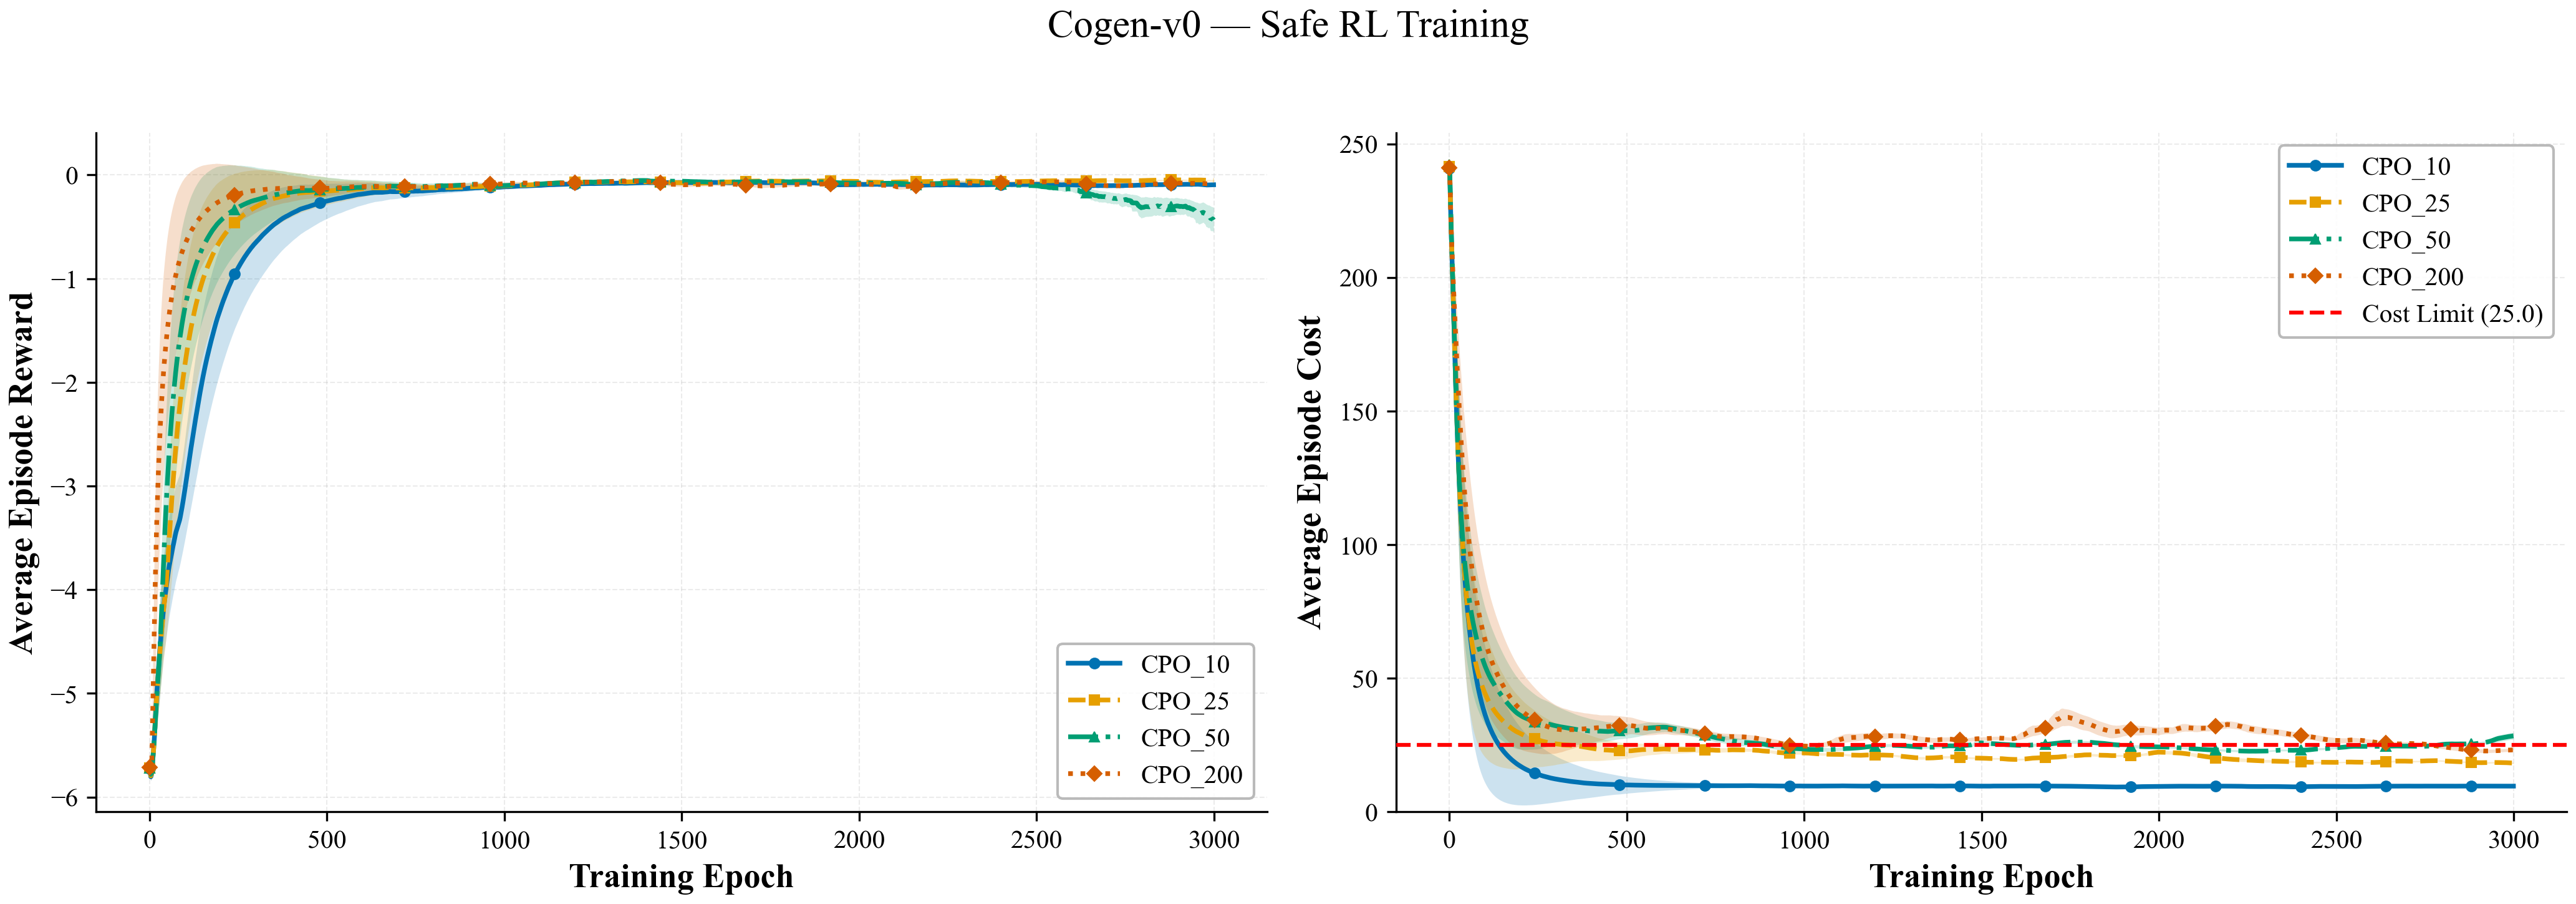
\includegraphics[width=0.9\textwidth]{figures/C_SRL/cogen/saferl_cogen_CPO_3000ep_200ema.png}
\caption{Cogen CPO: Training curves across four cost limits. Trust-region method converges rapidly but shows limited limit differentiation.}
\label{fig:srl_co_cpo}
\end{figure}

% --- Cogen OnCRPO ---
\subsubsection{Cogeneration --- OnCRPO}

OnCRPO shows similar behavior to CPO with rapid cost reduction but produces costs of $12$--$22$ across all four limits with minimal separation (\Cref{fig:srl_co_oncrpo}).

\begin{figure}[htbp]
\centering
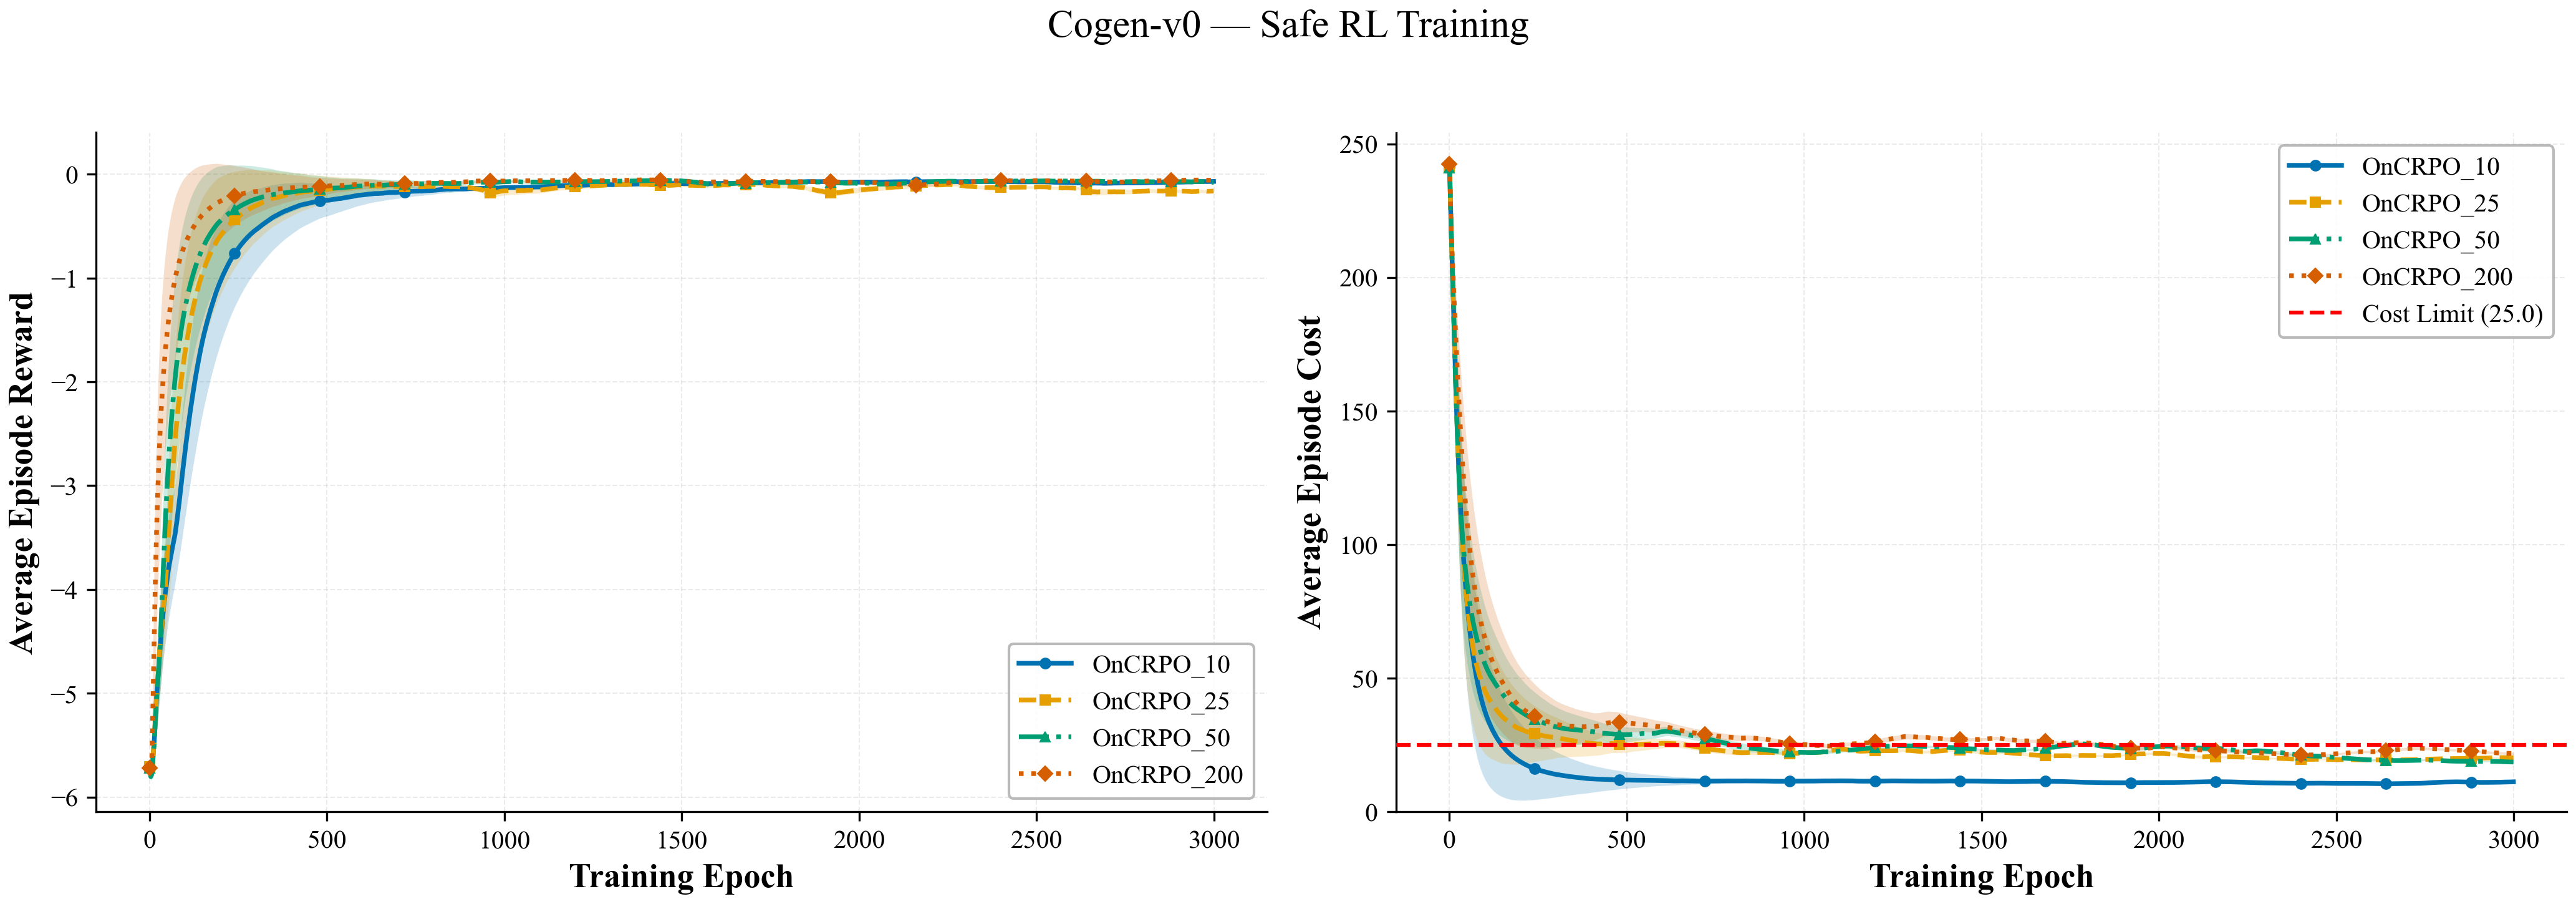
\includegraphics[width=0.9\textwidth]{figures/C_SRL/cogen/saferl_cogen_OnCRPO_3000ep_200ema.png}
\caption{Cogen OnCRPO: Rapid cost reduction but weak limit separation across all four cost limits.}
\label{fig:srl_co_oncrpo}
\end{figure}

% --- Cogen FOCOPS ---
\subsubsection{Cogeneration --- FOCOPS}

FOCOPS shows good monotonic differentiation ($d=10 \to 8$, $d=25 \to 17$, $d=50 \to 28$, $d=200 \to 51$) but converges more slowly than all other algorithms (\Cref{fig:srl_co_focops}).

\begin{figure}[htbp]
\centering
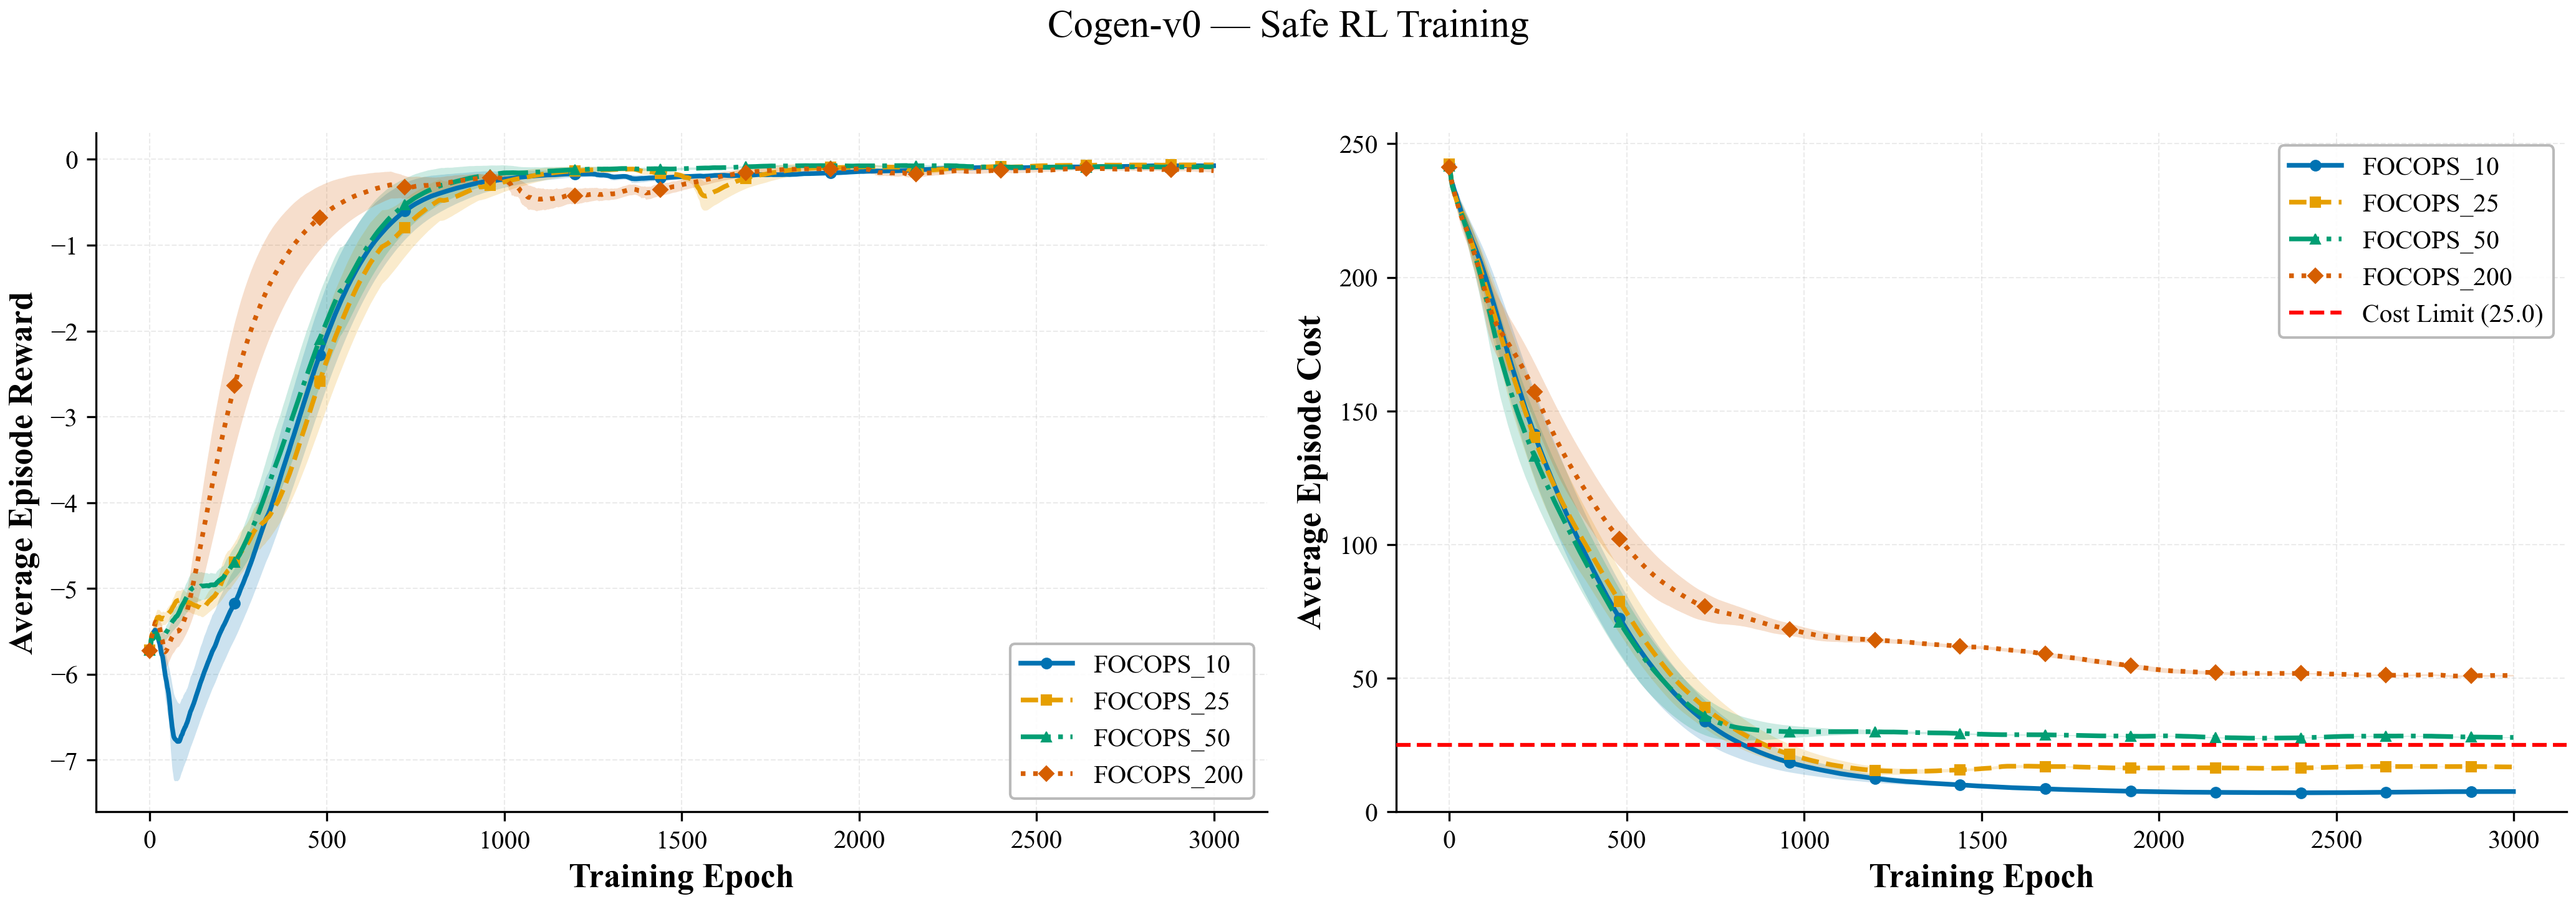
\includegraphics[width=0.9\textwidth]{figures/C_SRL/cogen/saferl_cogen_FOCOPS_3000ep_200ema.png}
\caption{Cogen FOCOPS: Slowest convergence but good monotonic cost differentiation.}
\label{fig:srl_co_focops}
\end{figure}

% --- Cogen Cross-Algorithm ---
\subsubsection{Cogeneration --- Cross-Algorithm Comparisons}

\Cref{fig:srl_co_cmp10,fig:cogen_compare,fig:srl_co_cmp50,fig:srl_co_cmp200} compare all four algorithms at each cost limit. At $d = 25$, the algorithm ranking is:
\begin{equation}
    \text{PPOLag} \succ \text{OnCRPO} \approx \text{CPO} \succ \text{FOCOPS}
\end{equation}

\begin{figure}[htbp]
\centering
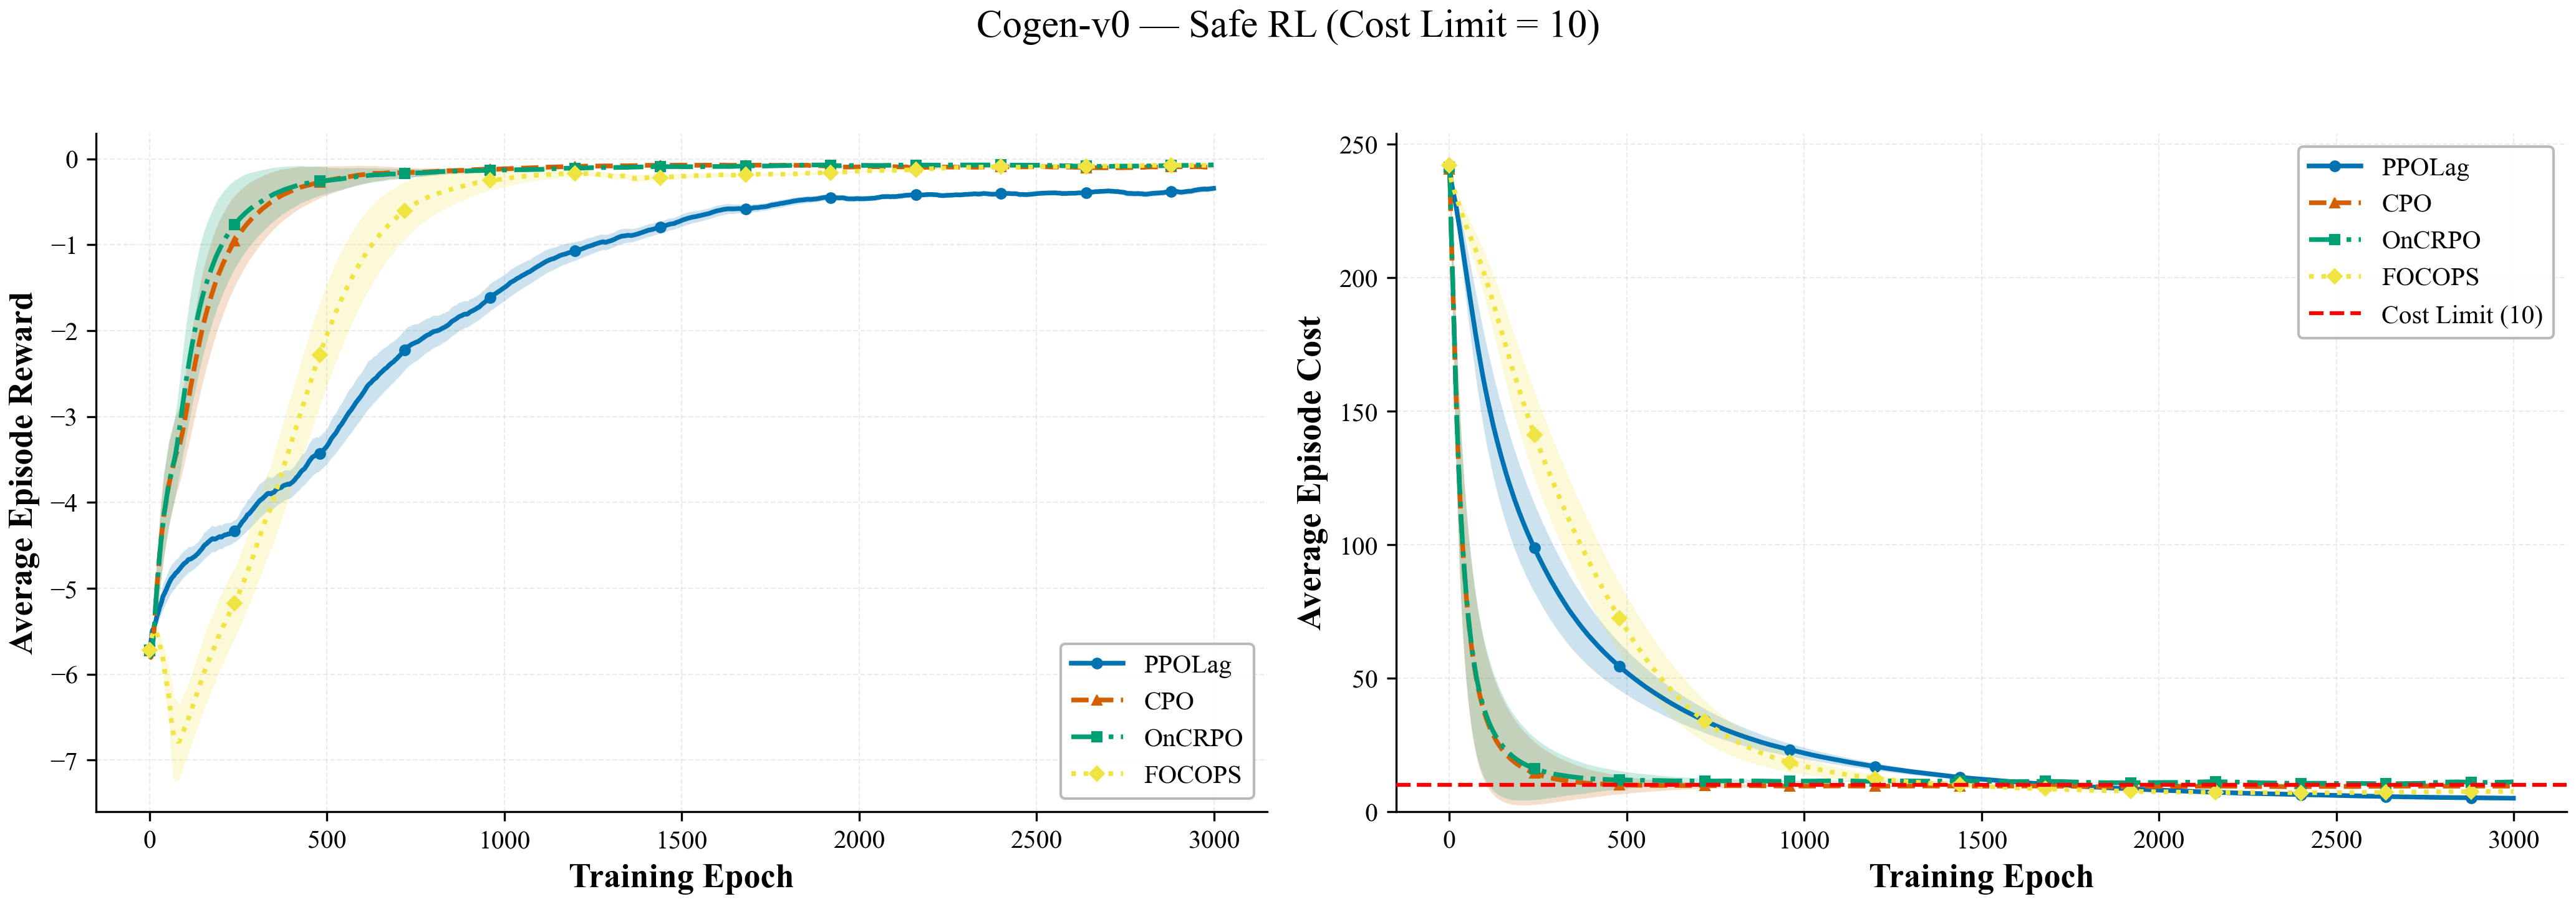
\includegraphics[width=0.9\textwidth]{figures/C_SRL/cogen/saferl_cogen_compare_CL10_3000ep_200ema.png}
\caption{Cogen cross-algorithm comparison at tightest limit $d = 10$.}
\label{fig:srl_co_cmp10}
\end{figure}

\begin{figure}[htbp]
\centering
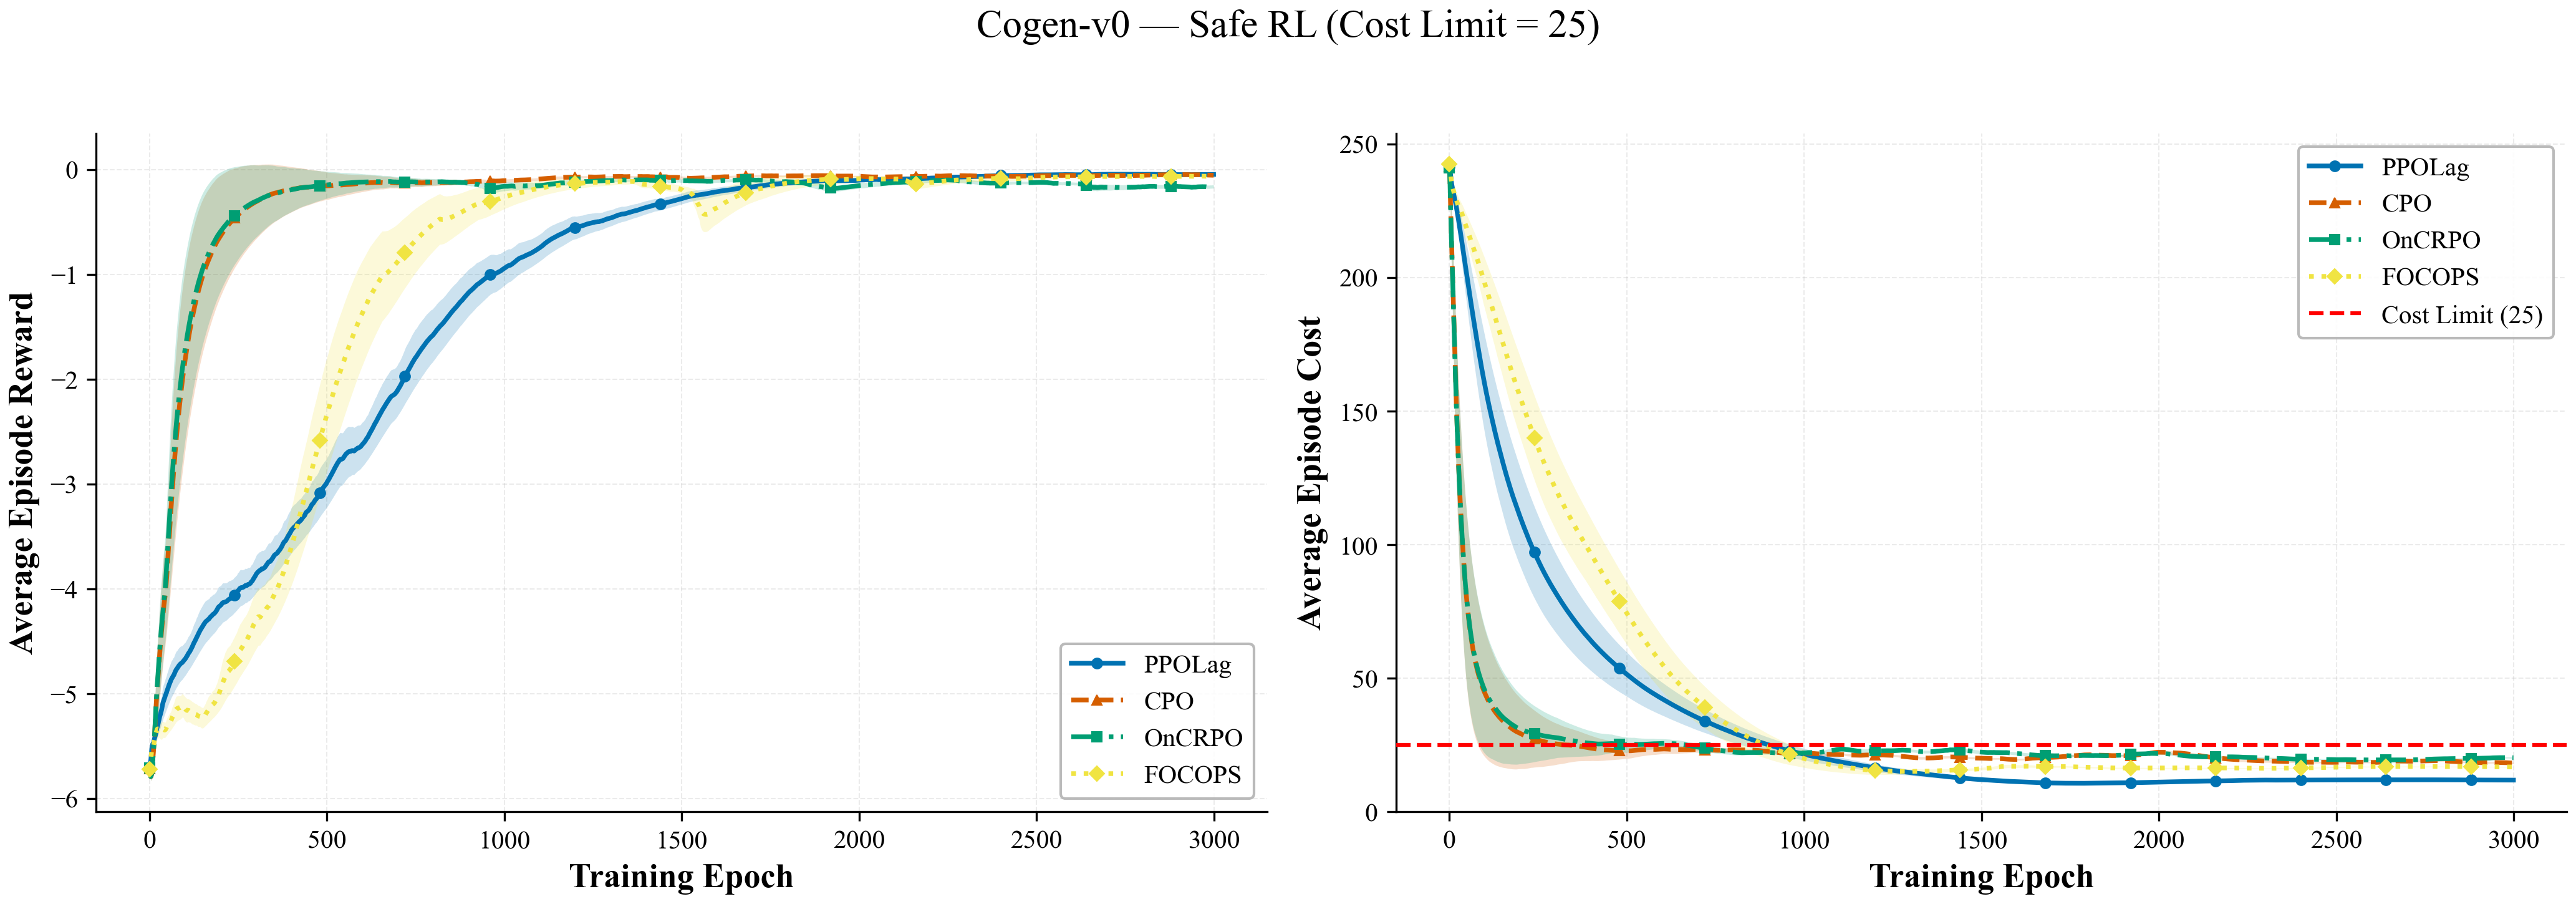
\includegraphics[width=0.9\textwidth]{figures/C_SRL/cogen/saferl_cogen_compare_CL25_3000ep_200ema.png}
\caption{Cogen cross-algorithm comparison at $d = 25$. PPOLag achieves the best reward while satisfying the constraint; FOCOPS converges slowest.}
\label{fig:cogen_compare}
\end{figure}

\begin{figure}[htbp]
\centering
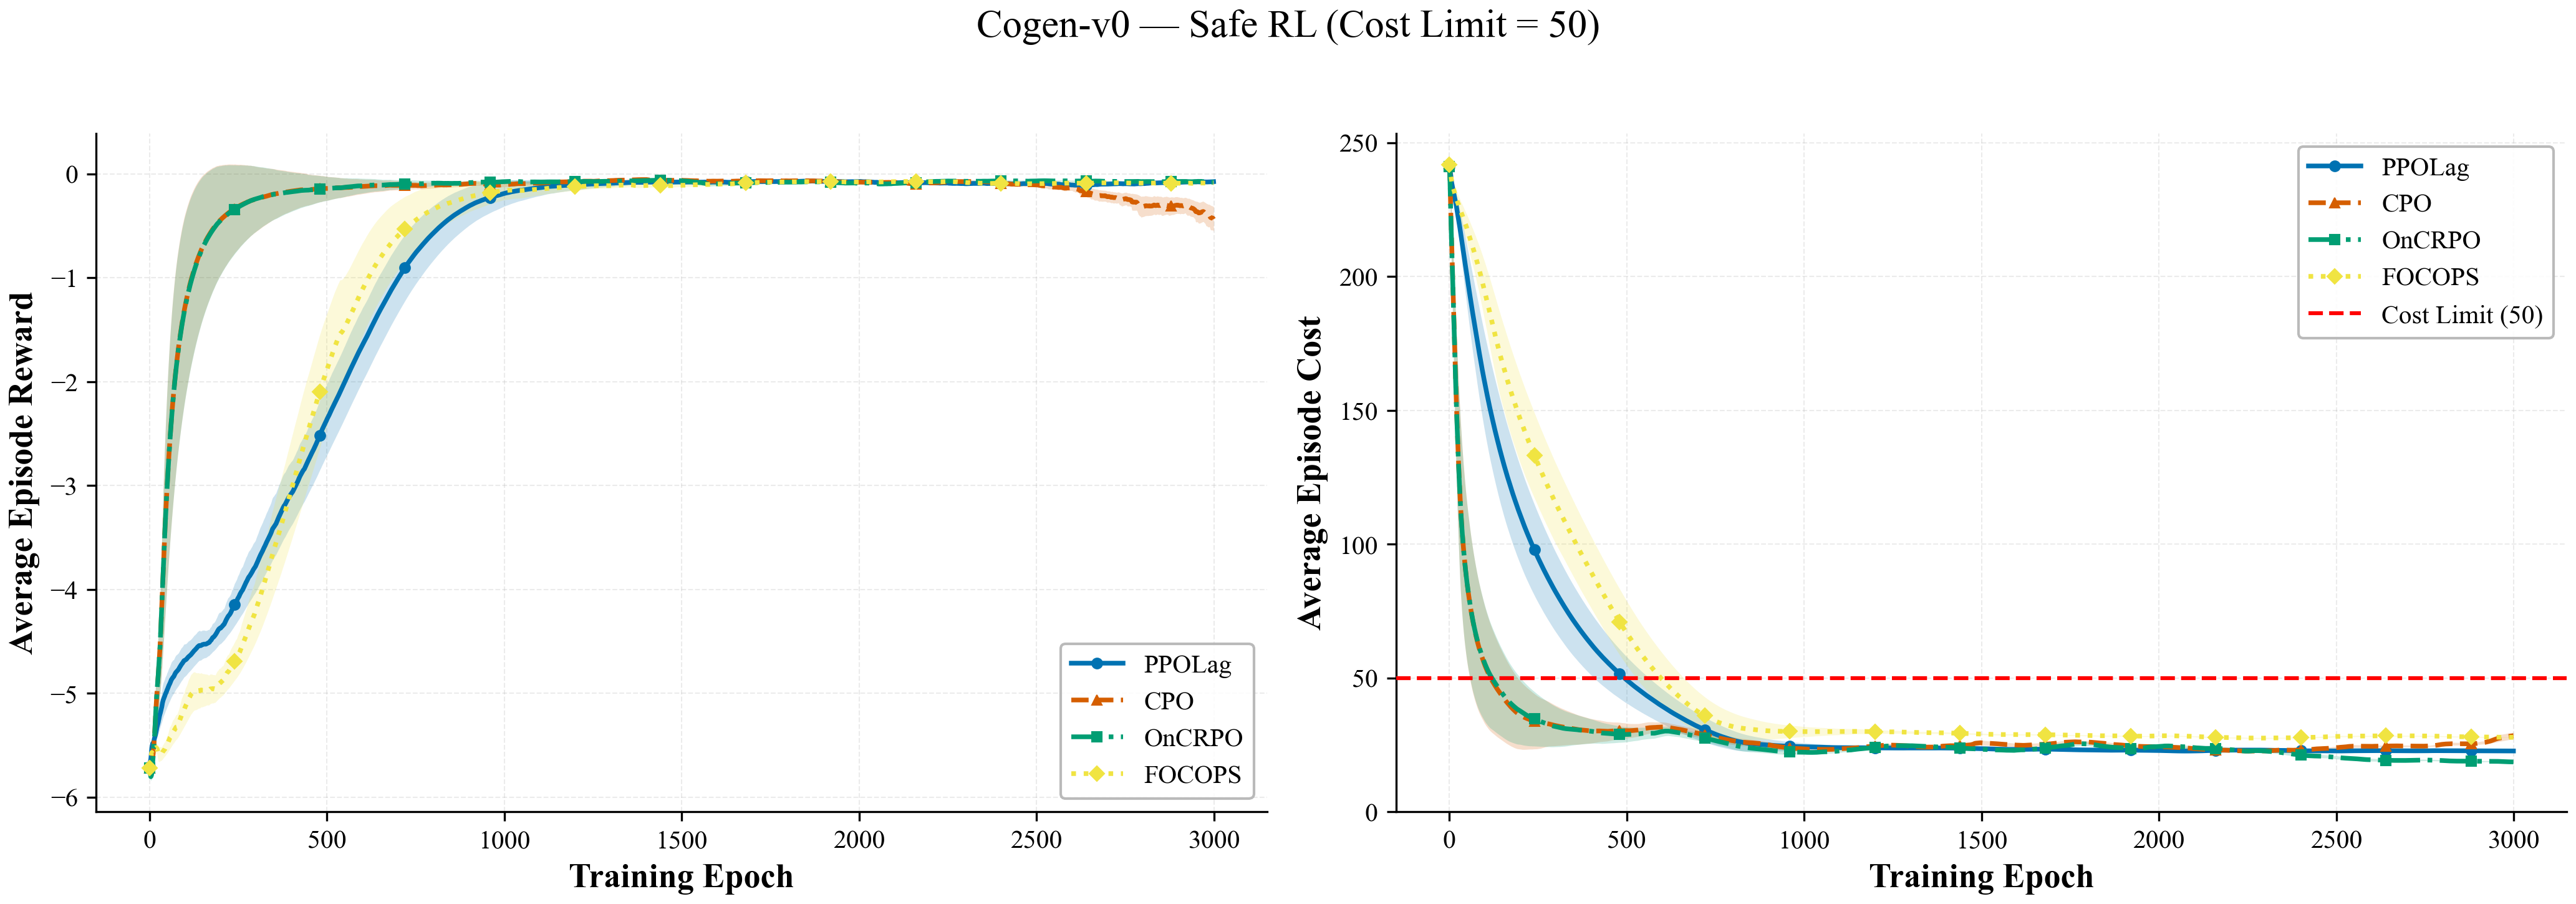
\includegraphics[width=0.9\textwidth]{figures/C_SRL/cogen/saferl_cogen_compare_CL50_3000ep_200ema.png}
\caption{Cogen cross-algorithm comparison at moderate limit $d = 50$.}
\label{fig:srl_co_cmp50}
\end{figure}

\begin{figure}[htbp]
\centering
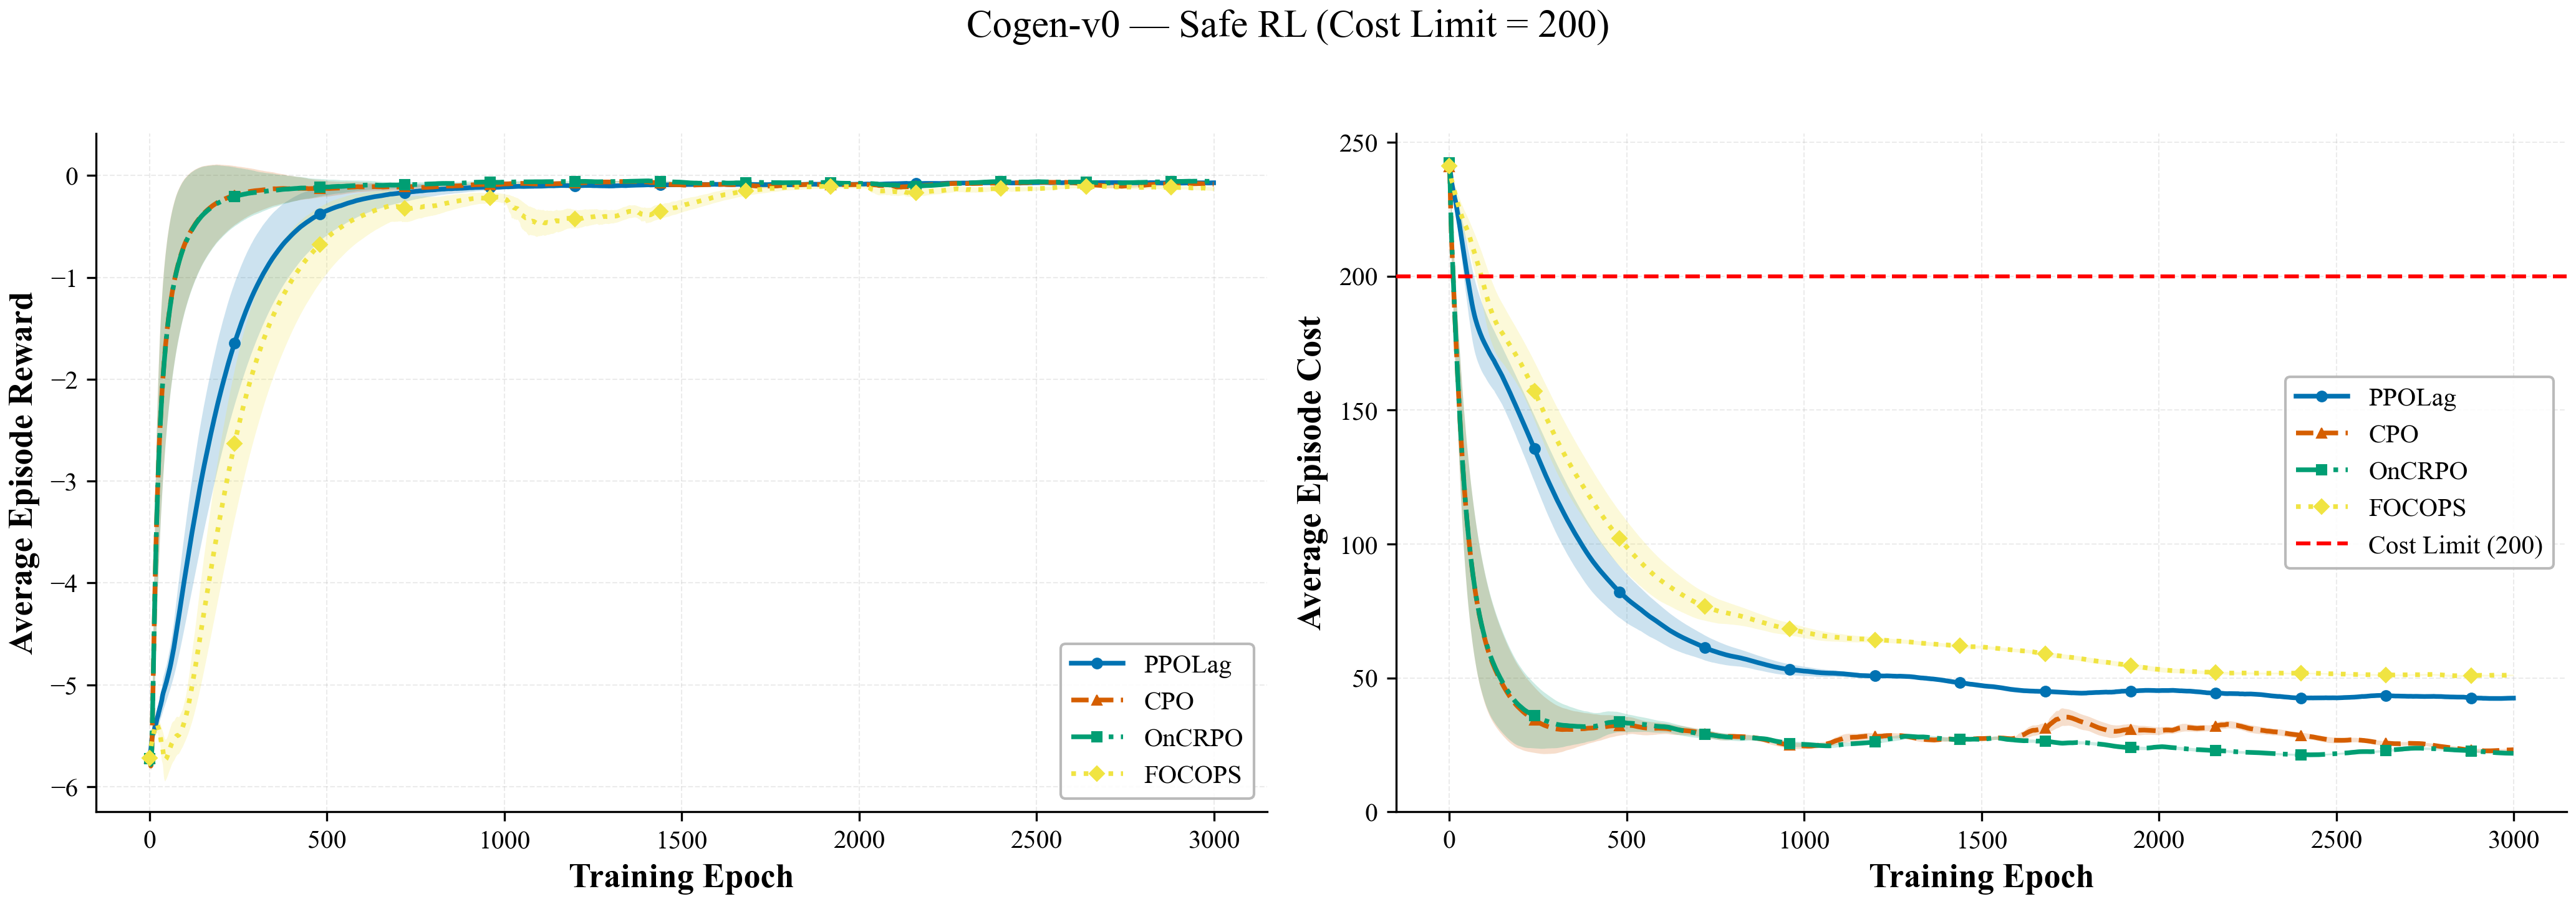
\includegraphics[width=0.9\textwidth]{figures/C_SRL/cogen/saferl_cogen_compare_CL200_3000ep_200ema.png}
\caption{Cogen cross-algorithm comparison at loosest limit $d = 200$.}
\label{fig:srl_co_cmp200}
\end{figure}

% ------------------------------------------------------------
\subsection{EV Charging: Precise Constraint Tracking}
\label{sec:saferl_ev}

The EV Charging CMDP cost (excess charge violations, $\alpha_c = 100$) is structurally orthogonal to the reward. With cost limits $d \in \{3, 5, 25\}$, all algorithms demonstrate strong constraint satisfaction (\Cref{tab:ev_saferl}).

\begin{table}[htbp]
\centering
\caption{EV Charging Safe RL: Final episode cost by algorithm and limit. \textbf{Bold}: satisfies $C \leq d$.}
\label{tab:ev_saferl}
\begin{tabular}{@{}lcccc@{}}
\toprule
\textbf{$d$} & \textbf{PPOLag} & \textbf{CPO} & \textbf{OnCRPO} & \textbf{FOCOPS} \\
\midrule
$3$  & $\mathbf{2.6}$ & $3.3$ & $4.5$ & $\mathbf{3.1}$ \\
$5$  & $\mathbf{5.1}$ & $\mathbf{5.7}$ & $6.9$ & $\mathbf{3.6}$ \\
$25$ & $\mathbf{21.5}$ & $\mathbf{20.7}$ & $27.5$ & $26.2$ \\
\bottomrule
\end{tabular}
\end{table}

% --- EV PPOLag ---
\subsubsection{EV Charging --- PPOLag}

PPOLag achieves near-exact constraint satisfaction at all levels (\Cref{fig:ev_ppolag}), demonstrating that Lagrangian relaxation provides precise control over network constraint violations. Tight limits ($d = 3, 5$) are precisely satisfied; loose limits ($d = 1000, 10000$) show natural cost reduction without active constraint enforcement.

\begin{figure}[htbp]
\centering
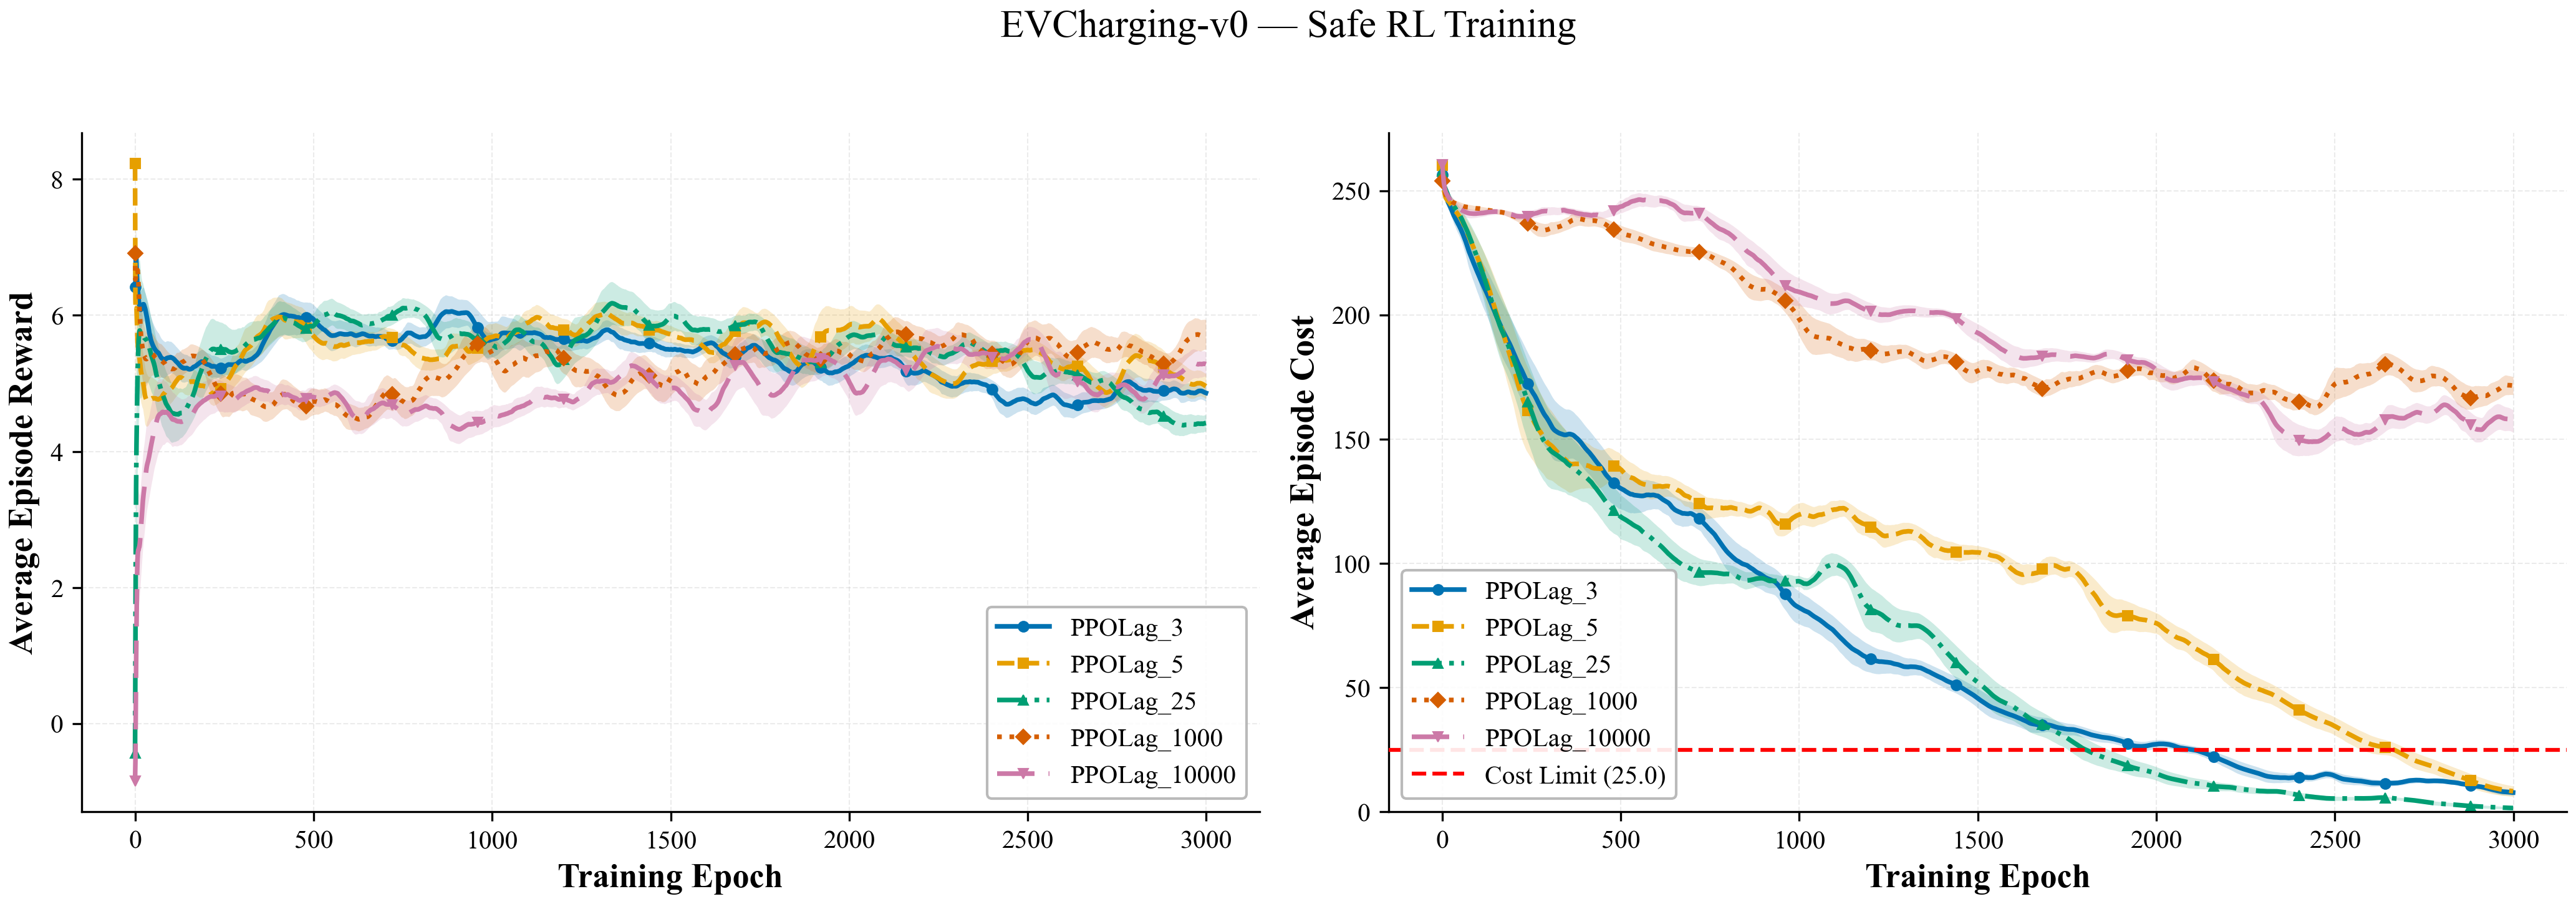
\includegraphics[width=0.9\textwidth]{figures/C_SRL/evcharging/saferl_evcharging_PPOLag_3000ep_200ema.png}
\caption{EV Charging PPOLag: Training curves across five cost limits. Tight limits ($d = 3, 5$) are precisely satisfied; loose limits show natural cost reduction.}
\label{fig:ev_ppolag}
\end{figure}

% --- EV CPO ---
\subsubsection{EV Charging --- CPO}

CPO satisfies the constraint at moderate and loose limits but slightly overshoots at the tightest limit ($d = 3$, final cost $= 3.3$), as shown in \Cref{fig:srl_ev_cpo}.

\begin{figure}[htbp]
\centering
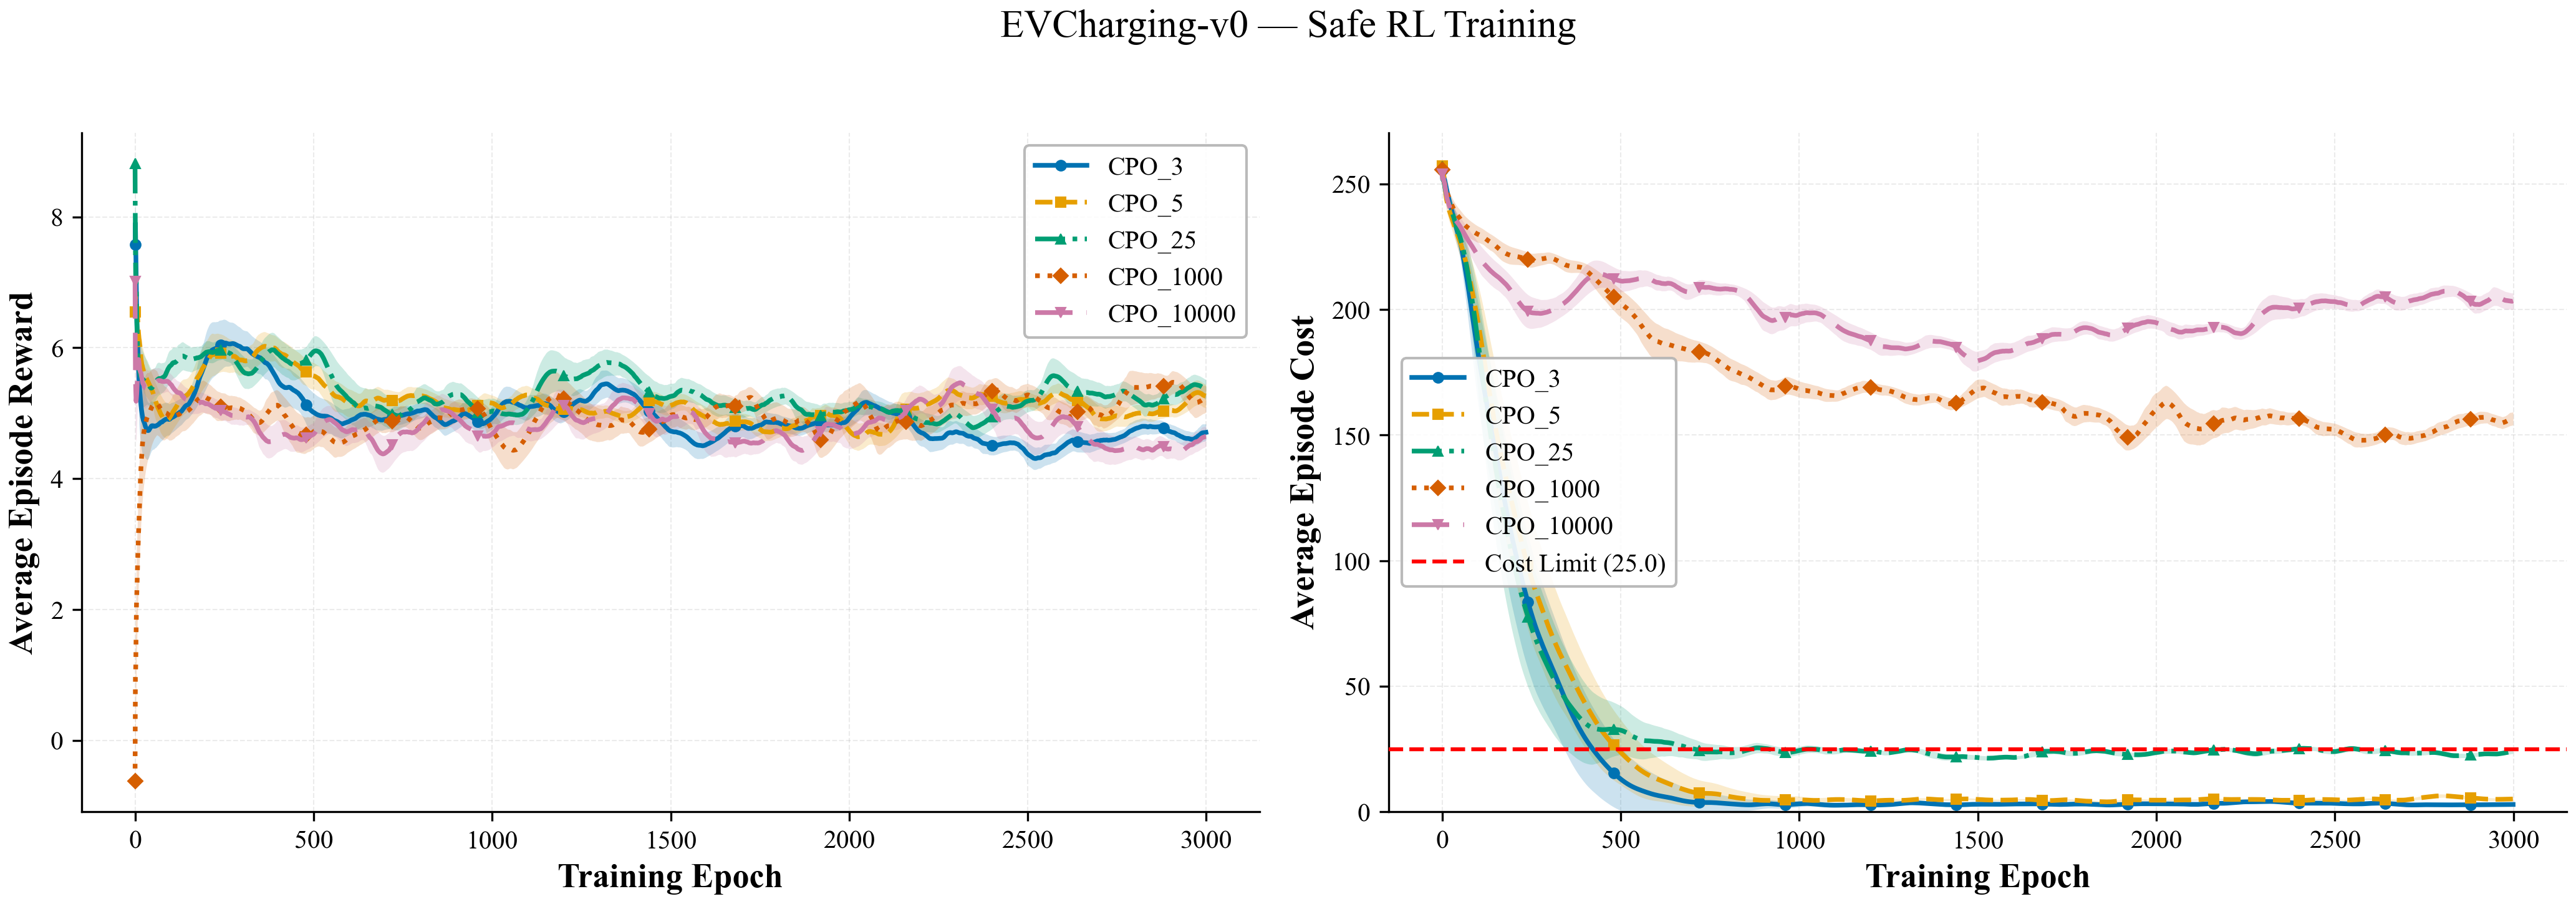
\includegraphics[width=0.9\textwidth]{figures/C_SRL/evcharging/saferl_evcharging_CPO_3000ep_200ema.png}
\caption{EV Charging CPO: Training curves across cost limits.}
\label{fig:srl_ev_cpo}
\end{figure}

% --- EV OnCRPO ---
\subsubsection{EV Charging --- OnCRPO}

OnCRPO consistently overshoots the prescribed cost limits (\Cref{fig:srl_ev_oncrpo}), with final costs exceeding the target at all three levels ($d = 3 \to 4.5$, $d = 5 \to 6.9$, $d = 25 \to 27.5$).

\begin{figure}[htbp]
\centering
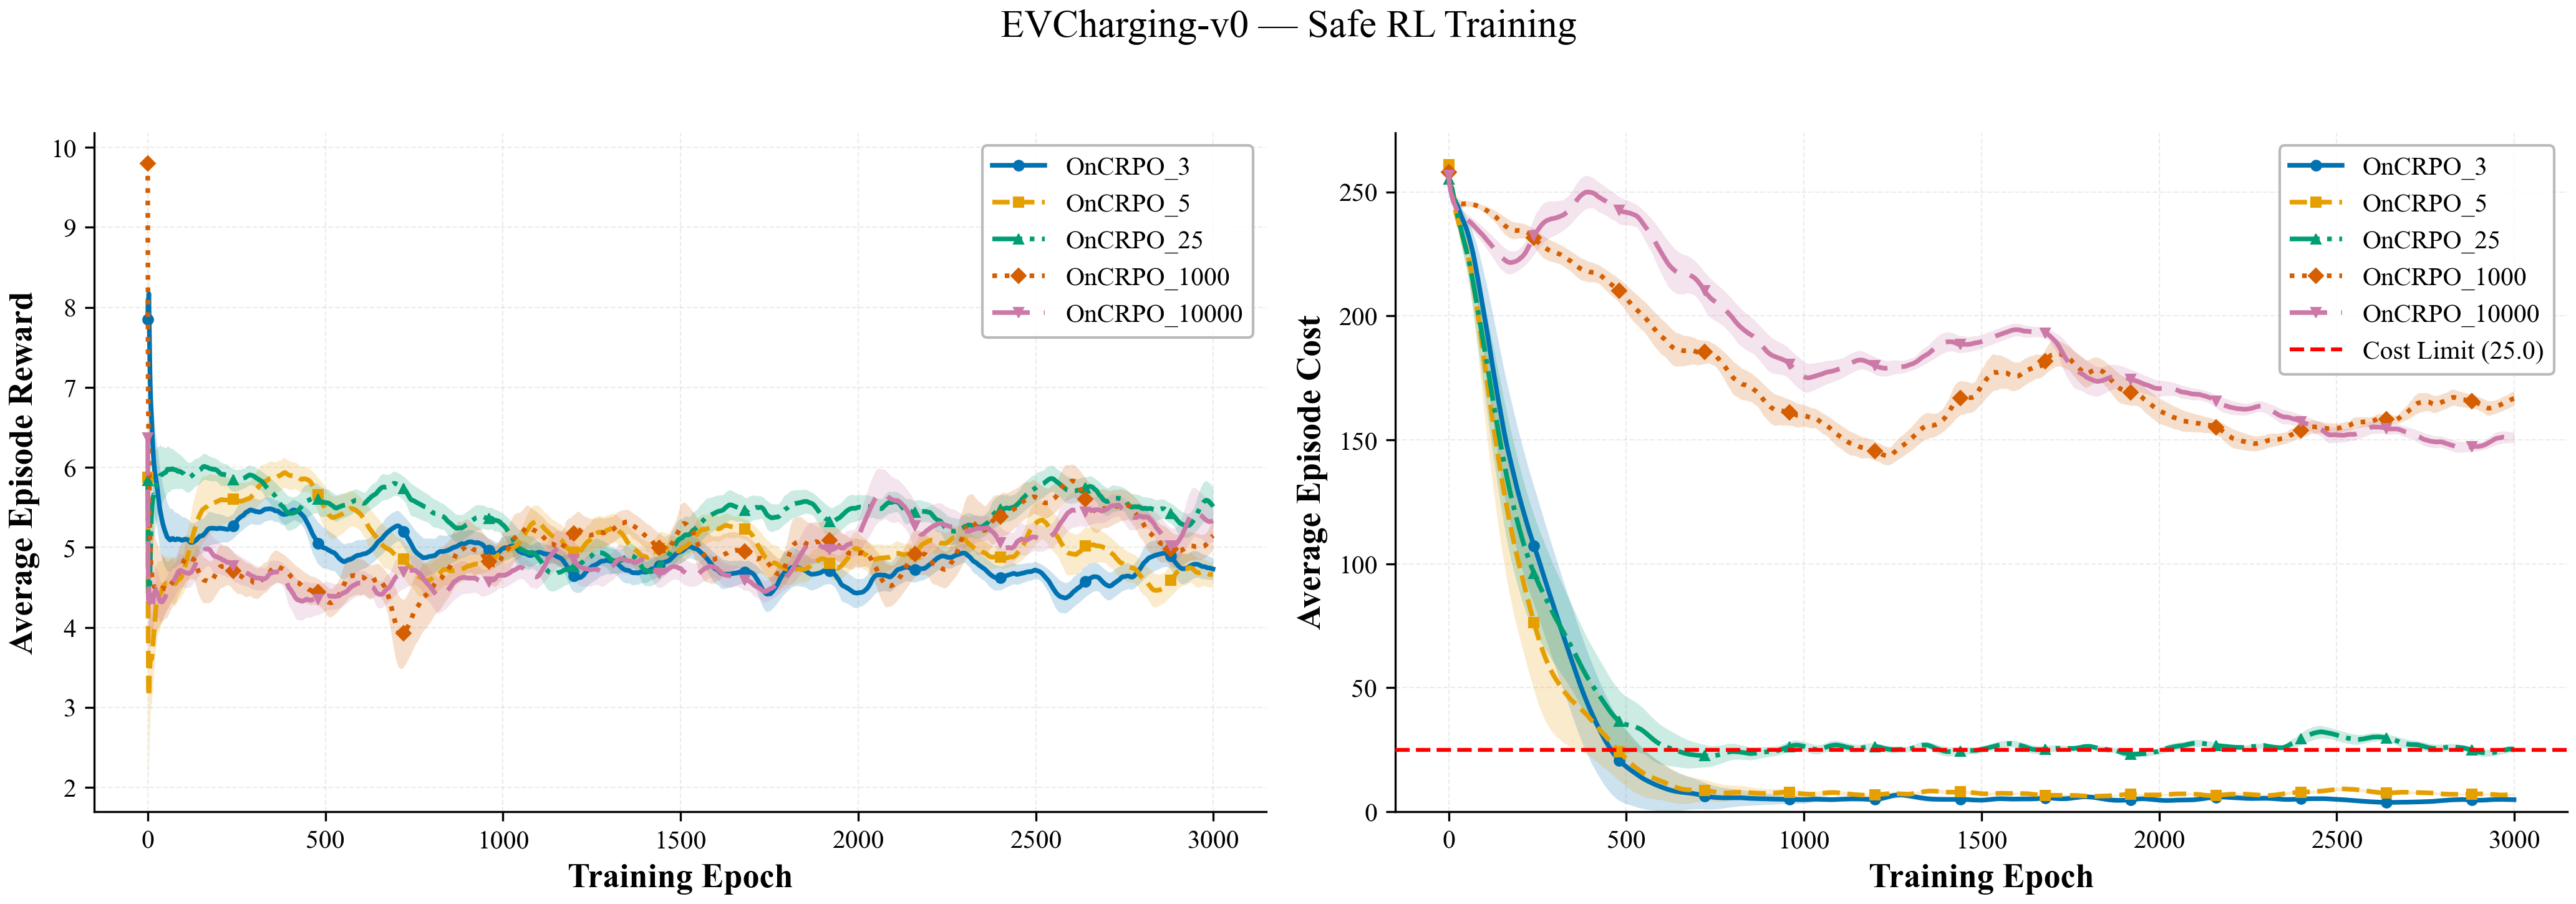
\includegraphics[width=0.9\textwidth]{figures/C_SRL/evcharging/saferl_evcharging_OnCRPO_3000ep_200ema.png}
\caption{EV Charging OnCRPO: Training curves across cost limits.}
\label{fig:srl_ev_oncrpo}
\end{figure}

% --- EV FOCOPS ---
\subsubsection{EV Charging --- FOCOPS}

FOCOPS achieves strong constraint satisfaction at tight limits ($d = 3 \to 3.1$, $d = 5 \to 3.6$) but slightly overshoots at loose limits ($d = 25 \to 26.2$), as shown in \Cref{fig:srl_ev_focops}.

\begin{figure}[htbp]
\centering
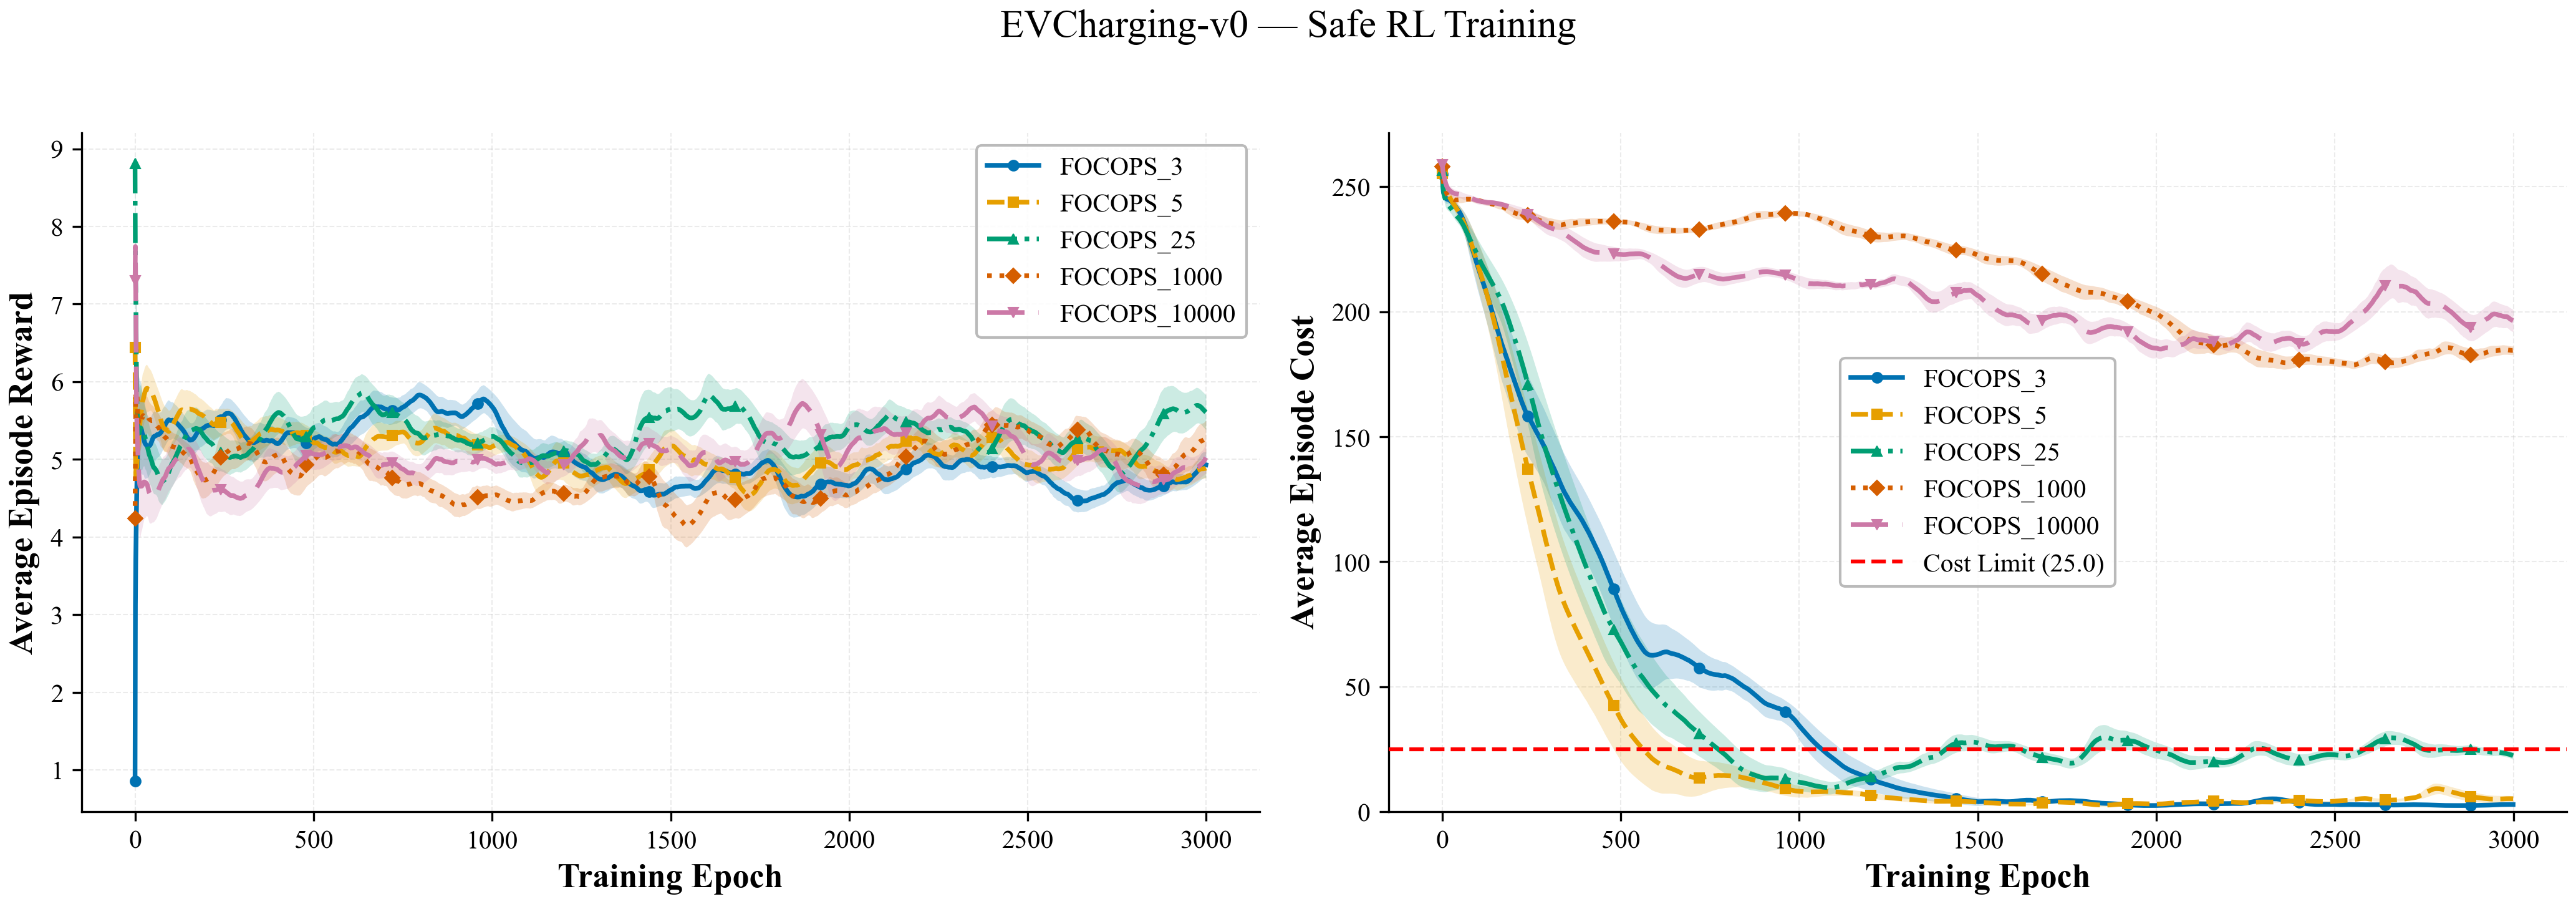
\includegraphics[width=0.9\textwidth]{figures/C_SRL/evcharging/saferl_evcharging_FOCOPS_3000ep_200ema.png}
\caption{EV Charging FOCOPS: Training curves across cost limits.}
\label{fig:srl_ev_focops}
\end{figure}

% --- EV Cross-Algorithm ---
\subsubsection{EV Charging --- Cross-Algorithm Comparisons}

\Cref{fig:srl_ev_cmp3,fig:srl_ev_cmp25} compare all four algorithms at the tightest and moderate cost limits respectively.

\begin{figure}[htbp]
\centering
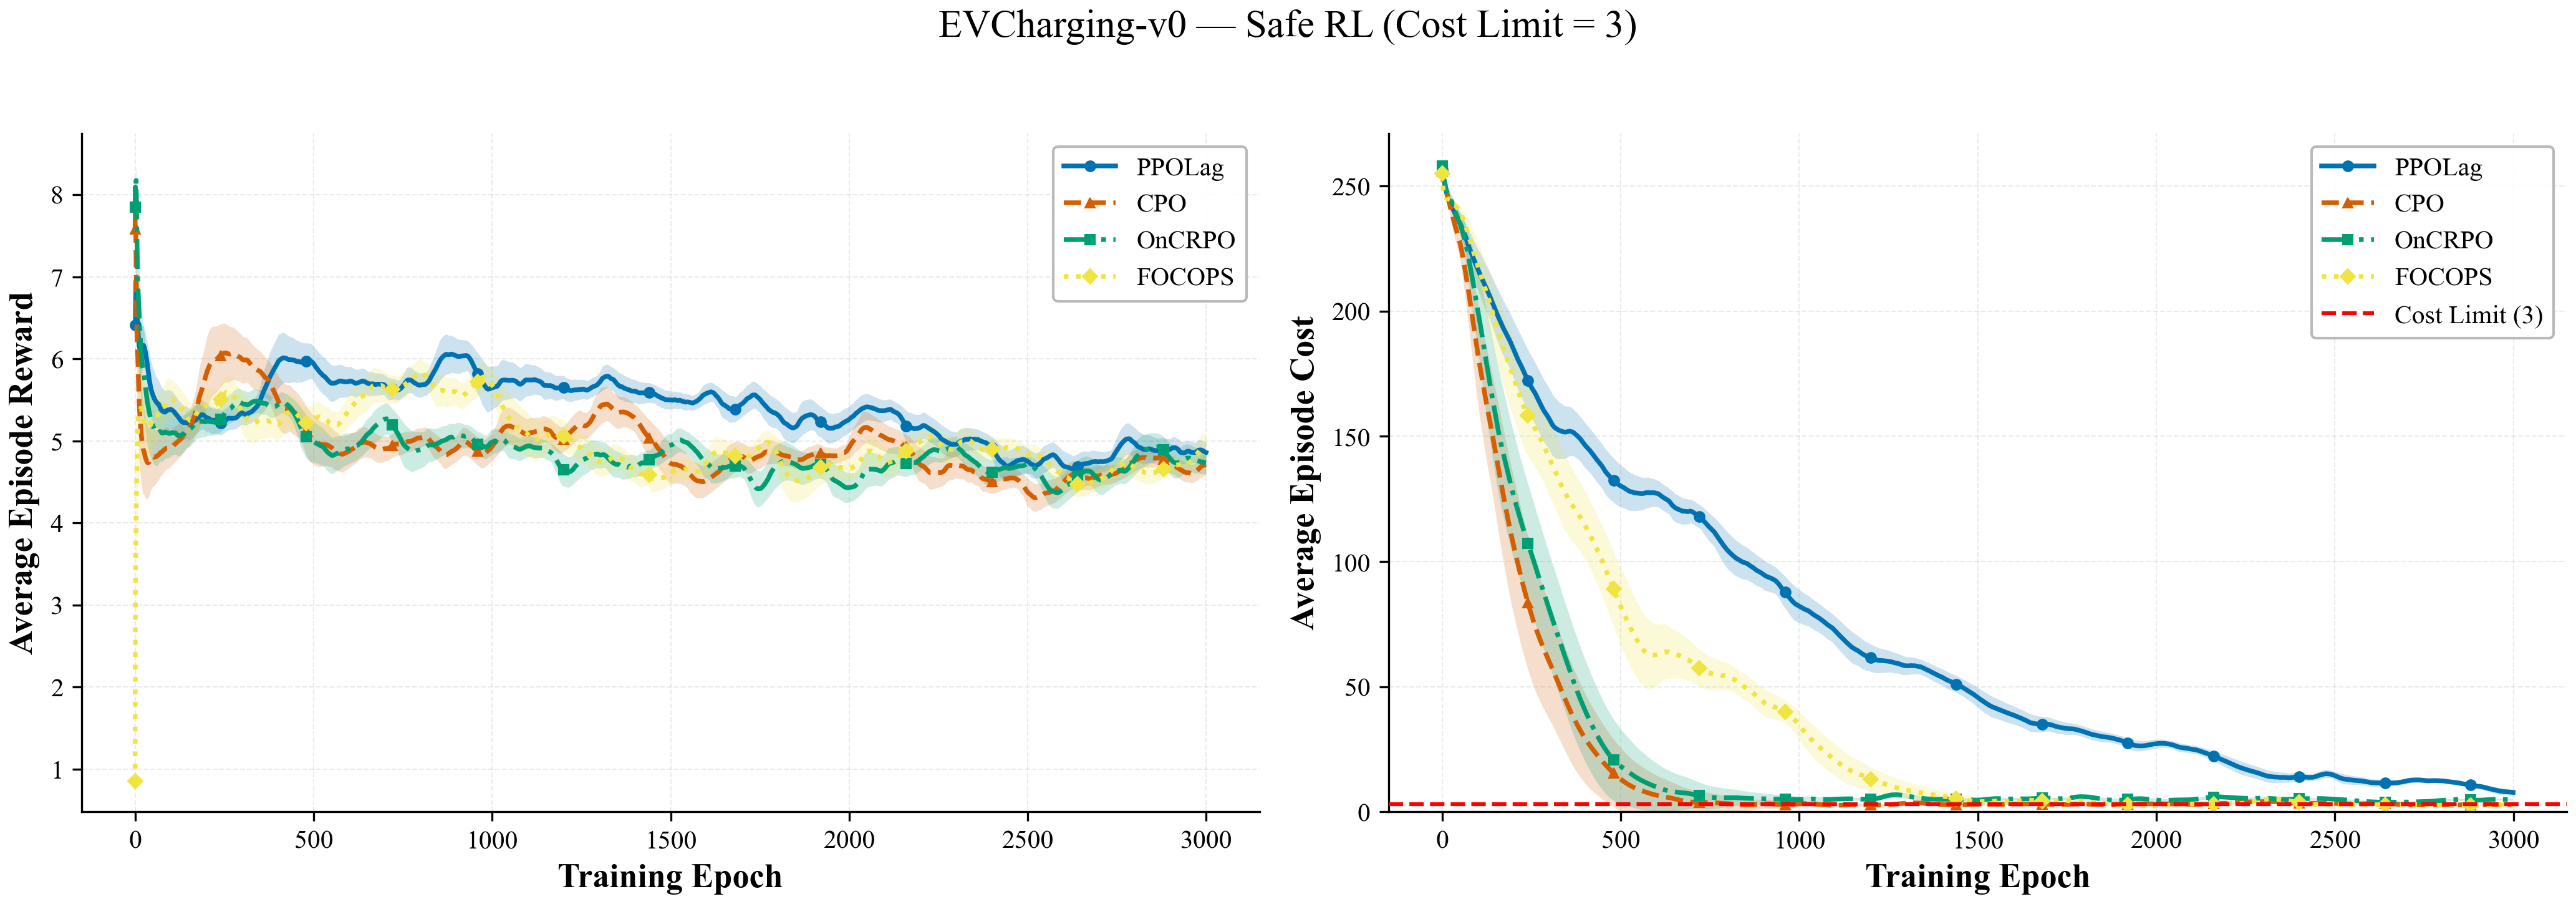
\includegraphics[width=0.9\textwidth]{figures/C_SRL/evcharging/saferl_evcharging_compare_CL3_3000ep_200ema.png}
\caption{EV Charging cross-algorithm comparison at tightest limit $d = 3$.}
\label{fig:srl_ev_cmp3}
\end{figure}

\begin{figure}[htbp]
\centering
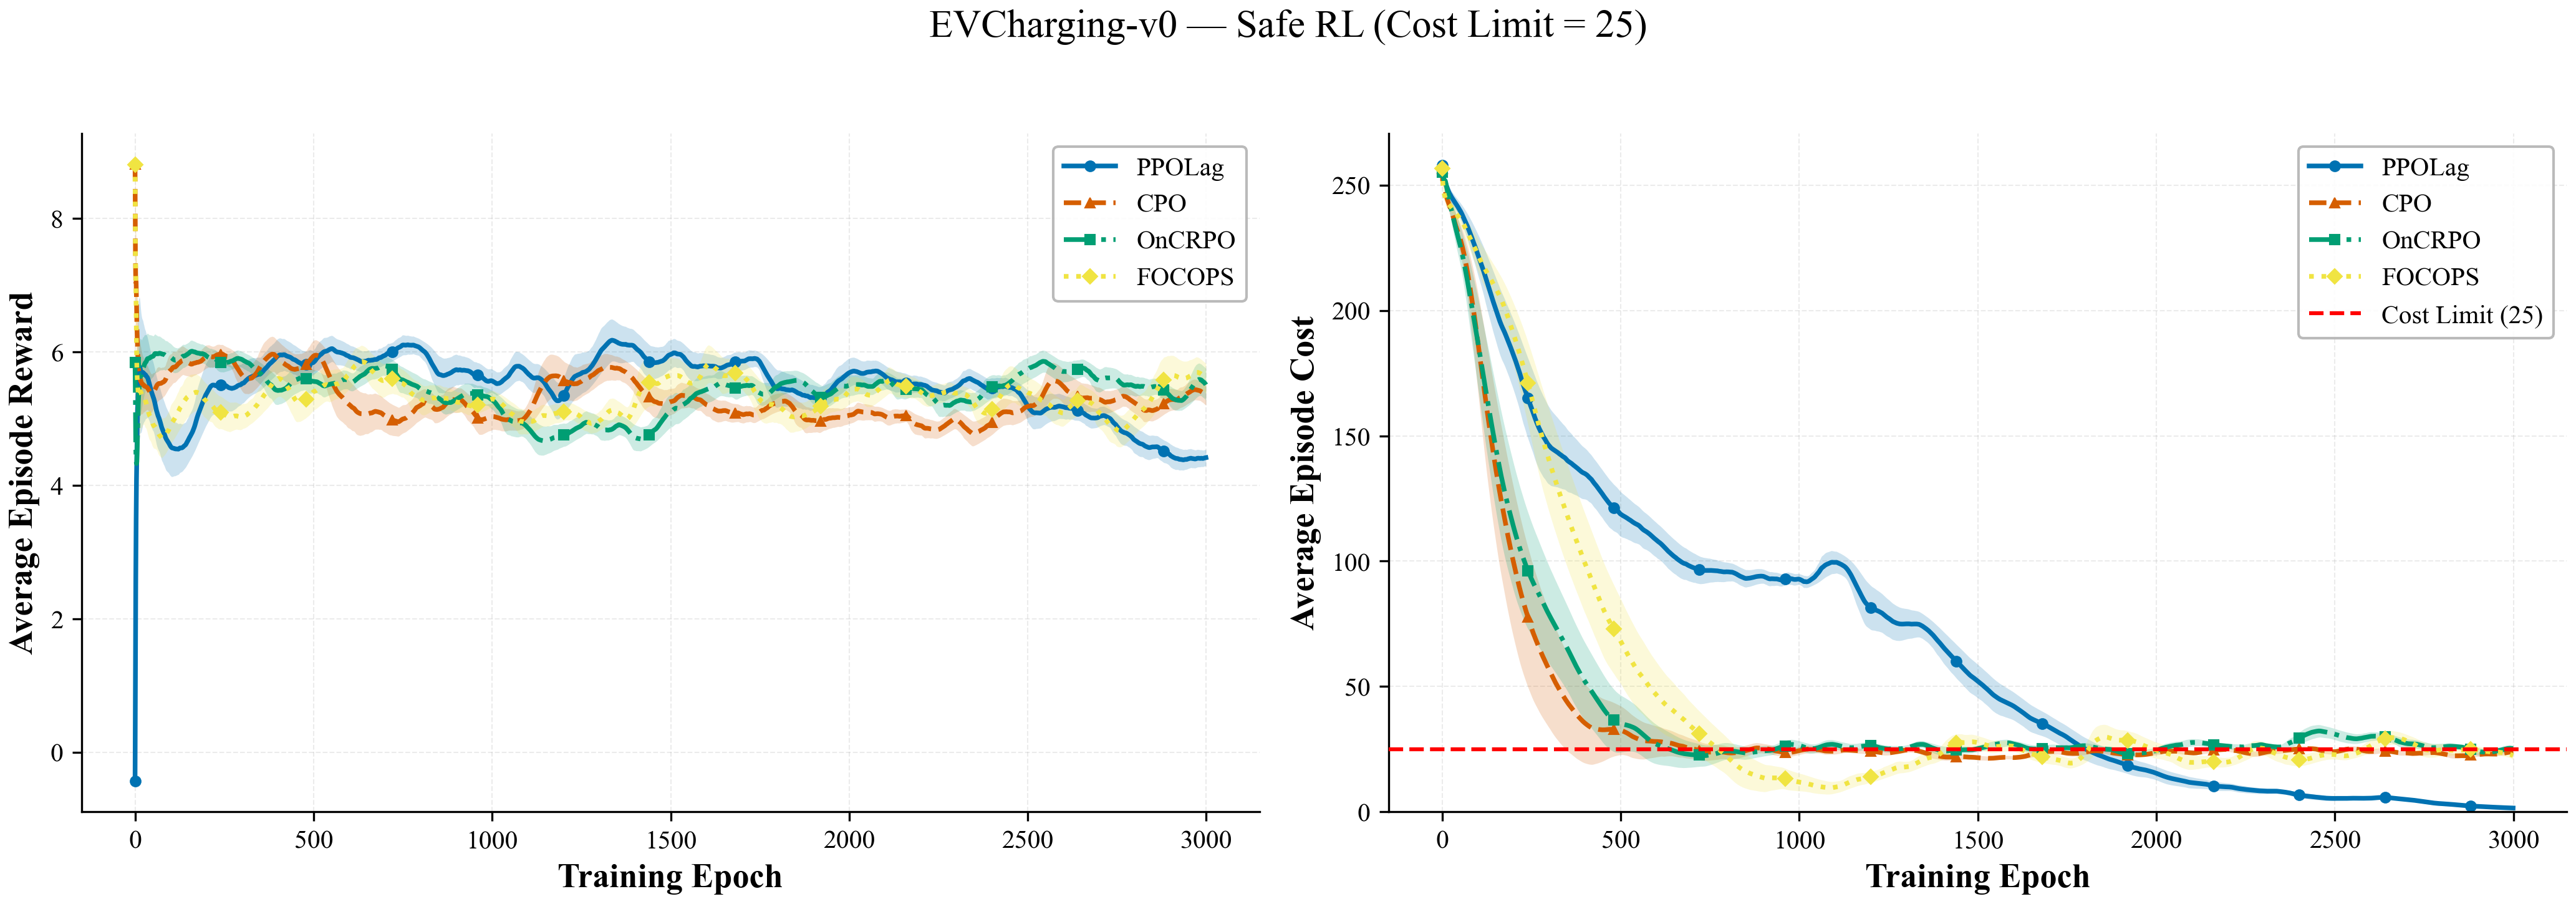
\includegraphics[width=0.9\textwidth]{figures/C_SRL/evcharging/saferl_evcharging_compare_CL25_3000ep_200ema.png}
\caption{EV Charging cross-algorithm comparison at moderate limit $d = 25$.}
\label{fig:srl_ev_cmp25}
\end{figure}

% ------------------------------------------------------------
\subsection{Building: A Negative Finding}
\label{sec:saferl_building}

Despite testing three cost function designs---raw temperature error, HVAC ramping, and deadband temperature violation---we were unable to achieve meaningful cost limit differentiation in the Building environment. \Cref{tab:building_saferl} summarizes the results.

\begin{table}[htbp]
\centering
\caption{Building Safe RL: PPOLag final episode cost across cost function designs. All limits converge to similar costs.}
\label{tab:building_saferl}
\begin{tabular}{@{}lcccc@{}}
\toprule
\textbf{Cost Function} & \textbf{$d_1$} & \textbf{$d_2$} & \textbf{$d_3$} & \textbf{$d_4$} \\
\midrule
Raw temp error & $6.7$ & $15.4$ & $12.4$ & $8.4$ \\
HVAC ramping & $6.5$ & $6.8$ & $7.2$ & $8.8$ \\
Deadband ($\delta = 1$\textdegree C) & $2.1$ & $2.3$ & $1.8$ & $2.5$ \\
\bottomrule
\end{tabular}
\end{table}

The root cause is a \emph{reward--cost alignment problem}: the reward function with $\beta = 0.5$ already strongly incentivizes both energy efficiency and thermal comfort. The agent minimizes temperature errors through reward optimization alone, trivially satisfying any temperature-based CMDP constraint.

% --- Building PPOLag ---
\subsubsection{Building --- PPOLag}

All four cost limits produce nearly identical training curves (\Cref{fig:building_ppolag}), with episode cost collapsing to $\approx 2$--$5$ regardless of the prescribed limit.

\begin{figure}[htbp]
\centering
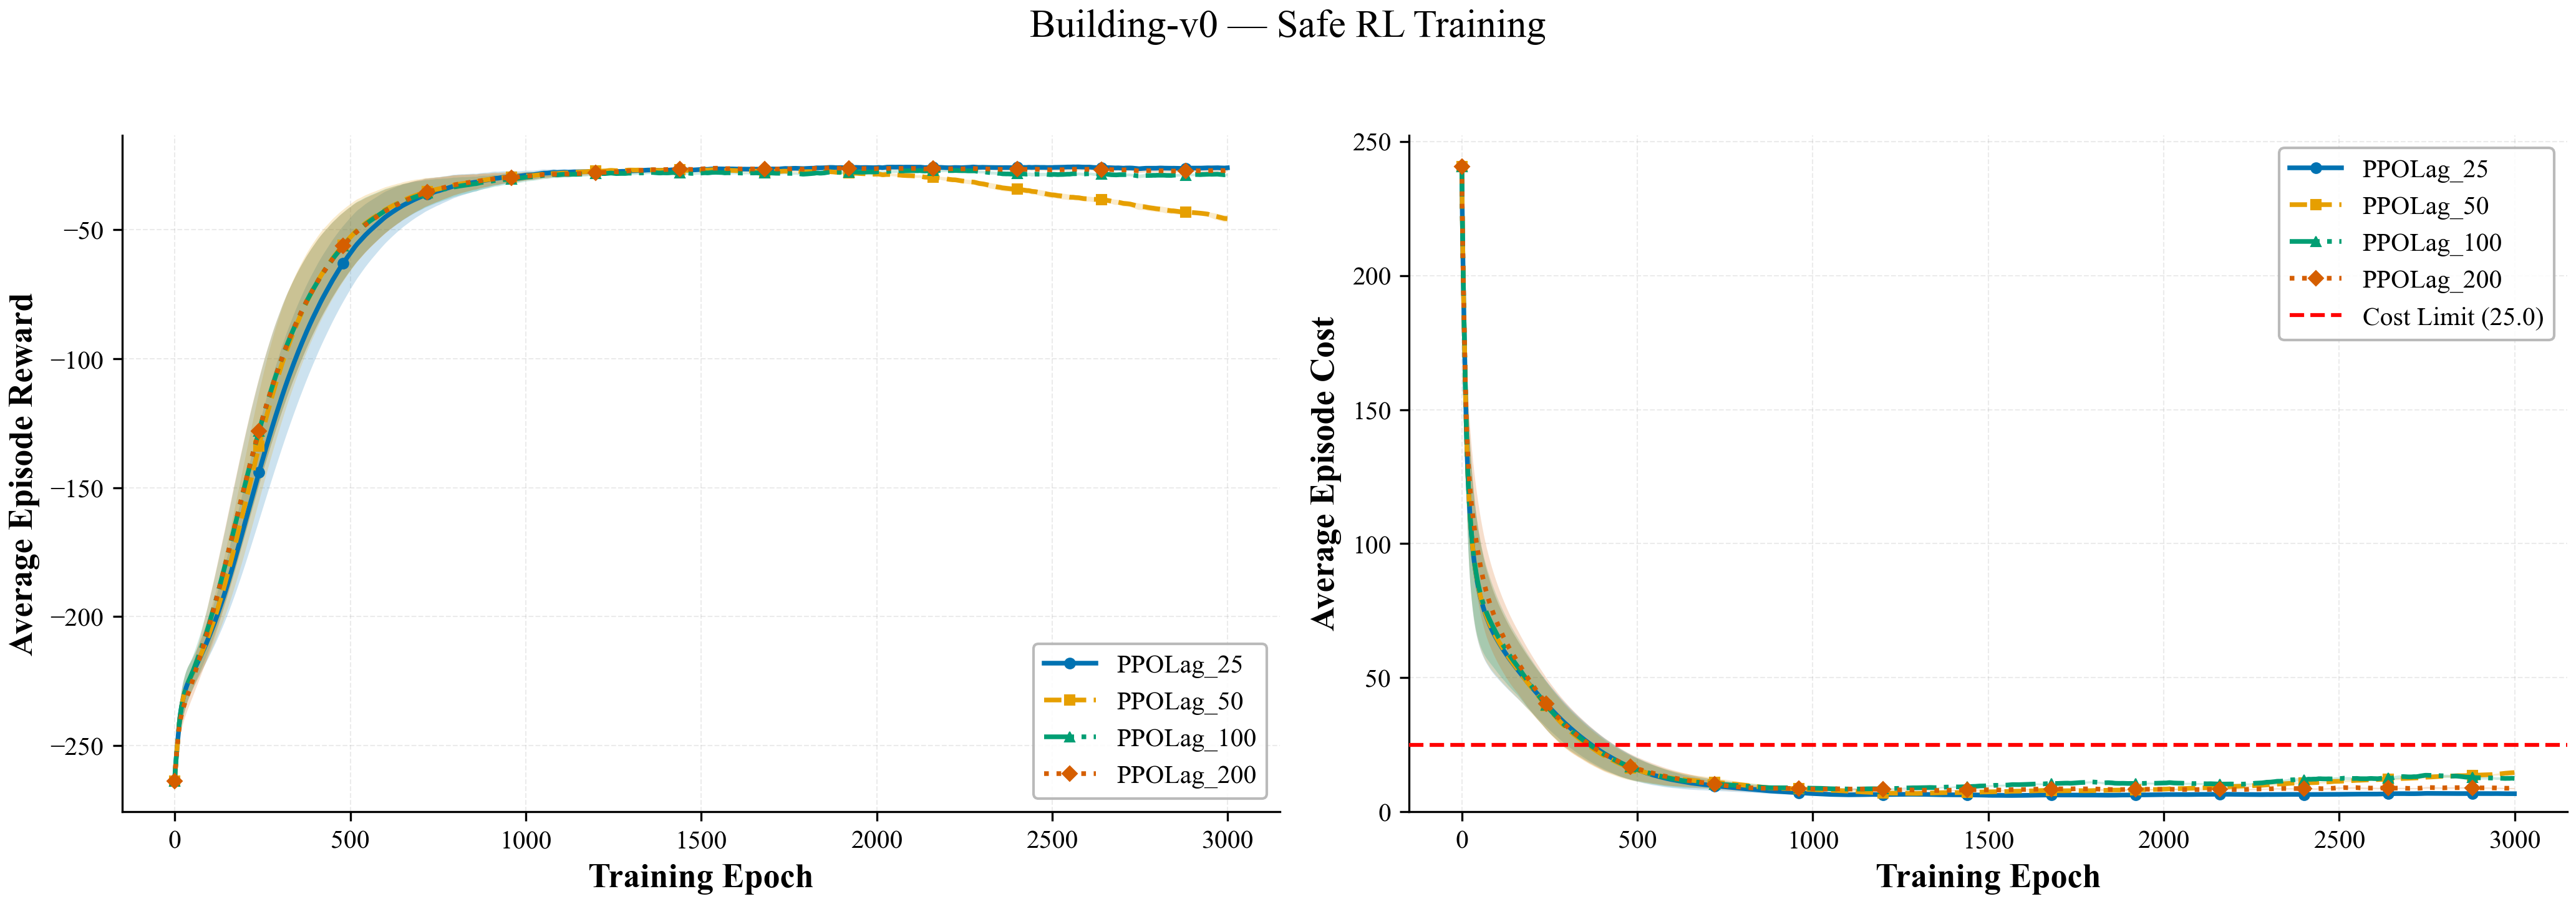
\includegraphics[width=0.9\textwidth]{figures/C_SRL/building/saferl_building_PPOLag_3000ep_200ema.png}
\caption{Building PPOLag: All four cost limits produce nearly identical training curves, demonstrating the absence of constraint differentiation.}
\label{fig:building_ppolag}
\end{figure}

% --- Building CPO ---
\subsubsection{Building --- CPO}

CPO exhibits divergence at loose limits ($d = 200, 500$), while tight limits lack differentiation (\Cref{fig:srl_bu_cpo}). This confirms the trust-region instability under nearly inactive constraints.

\begin{figure}[htbp]
\centering
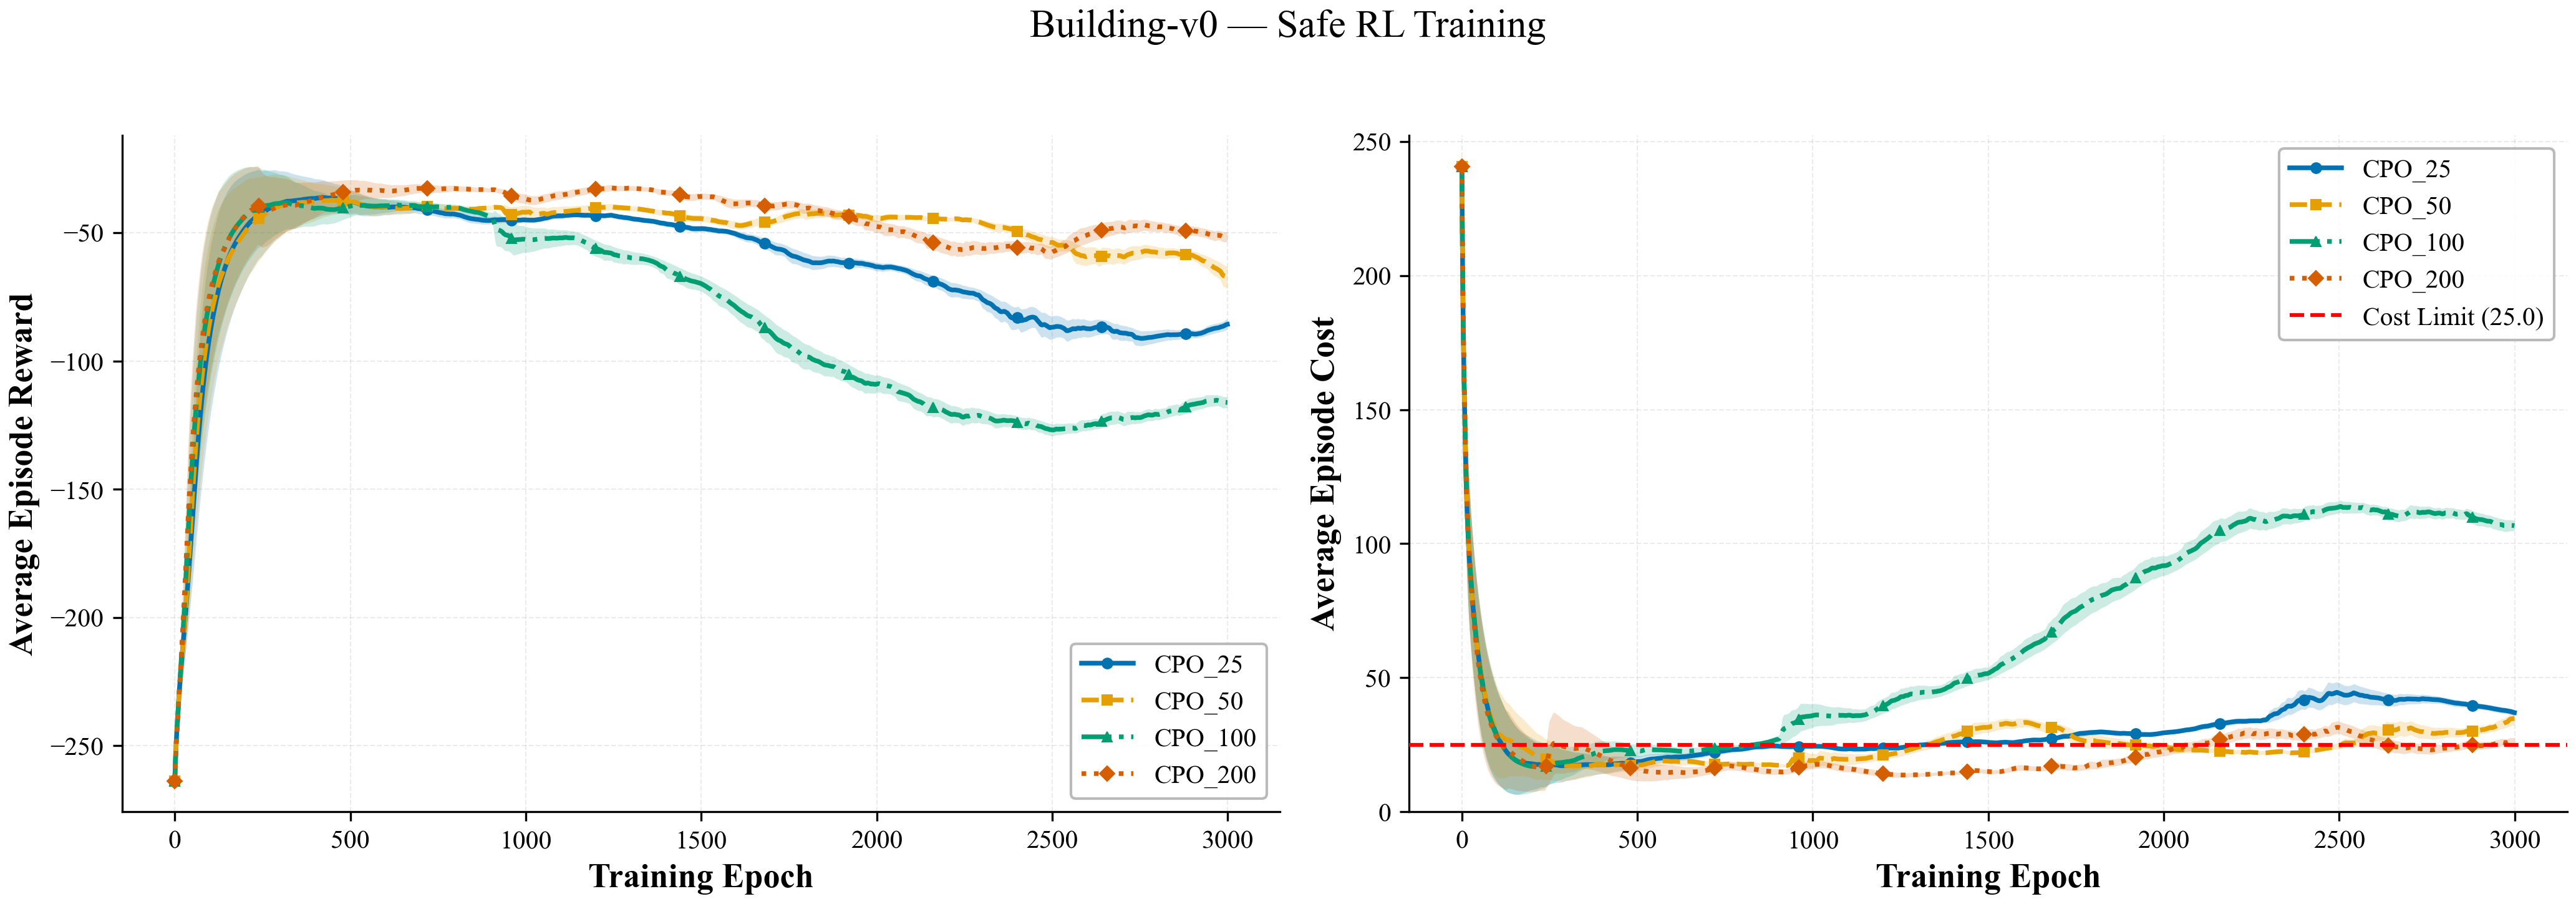
\includegraphics[width=0.9\textwidth]{figures/C_SRL/building/saferl_building_CPO_3000ep_200ema.png}
\caption{Building CPO: Loose limits ($d = 200, 500$) diverge; tight limits lack differentiation.}
\label{fig:srl_bu_cpo}
\end{figure}

% --- Building OnCRPO ---
\subsubsection{Building --- OnCRPO}

OnCRPO shows a similar divergence pattern to CPO at loose limits (\Cref{fig:srl_bu_oncrpo}), further confirming that trust-region CMDP methods are unstable when constraints are nearly inactive.

\begin{figure}[htbp]
\centering
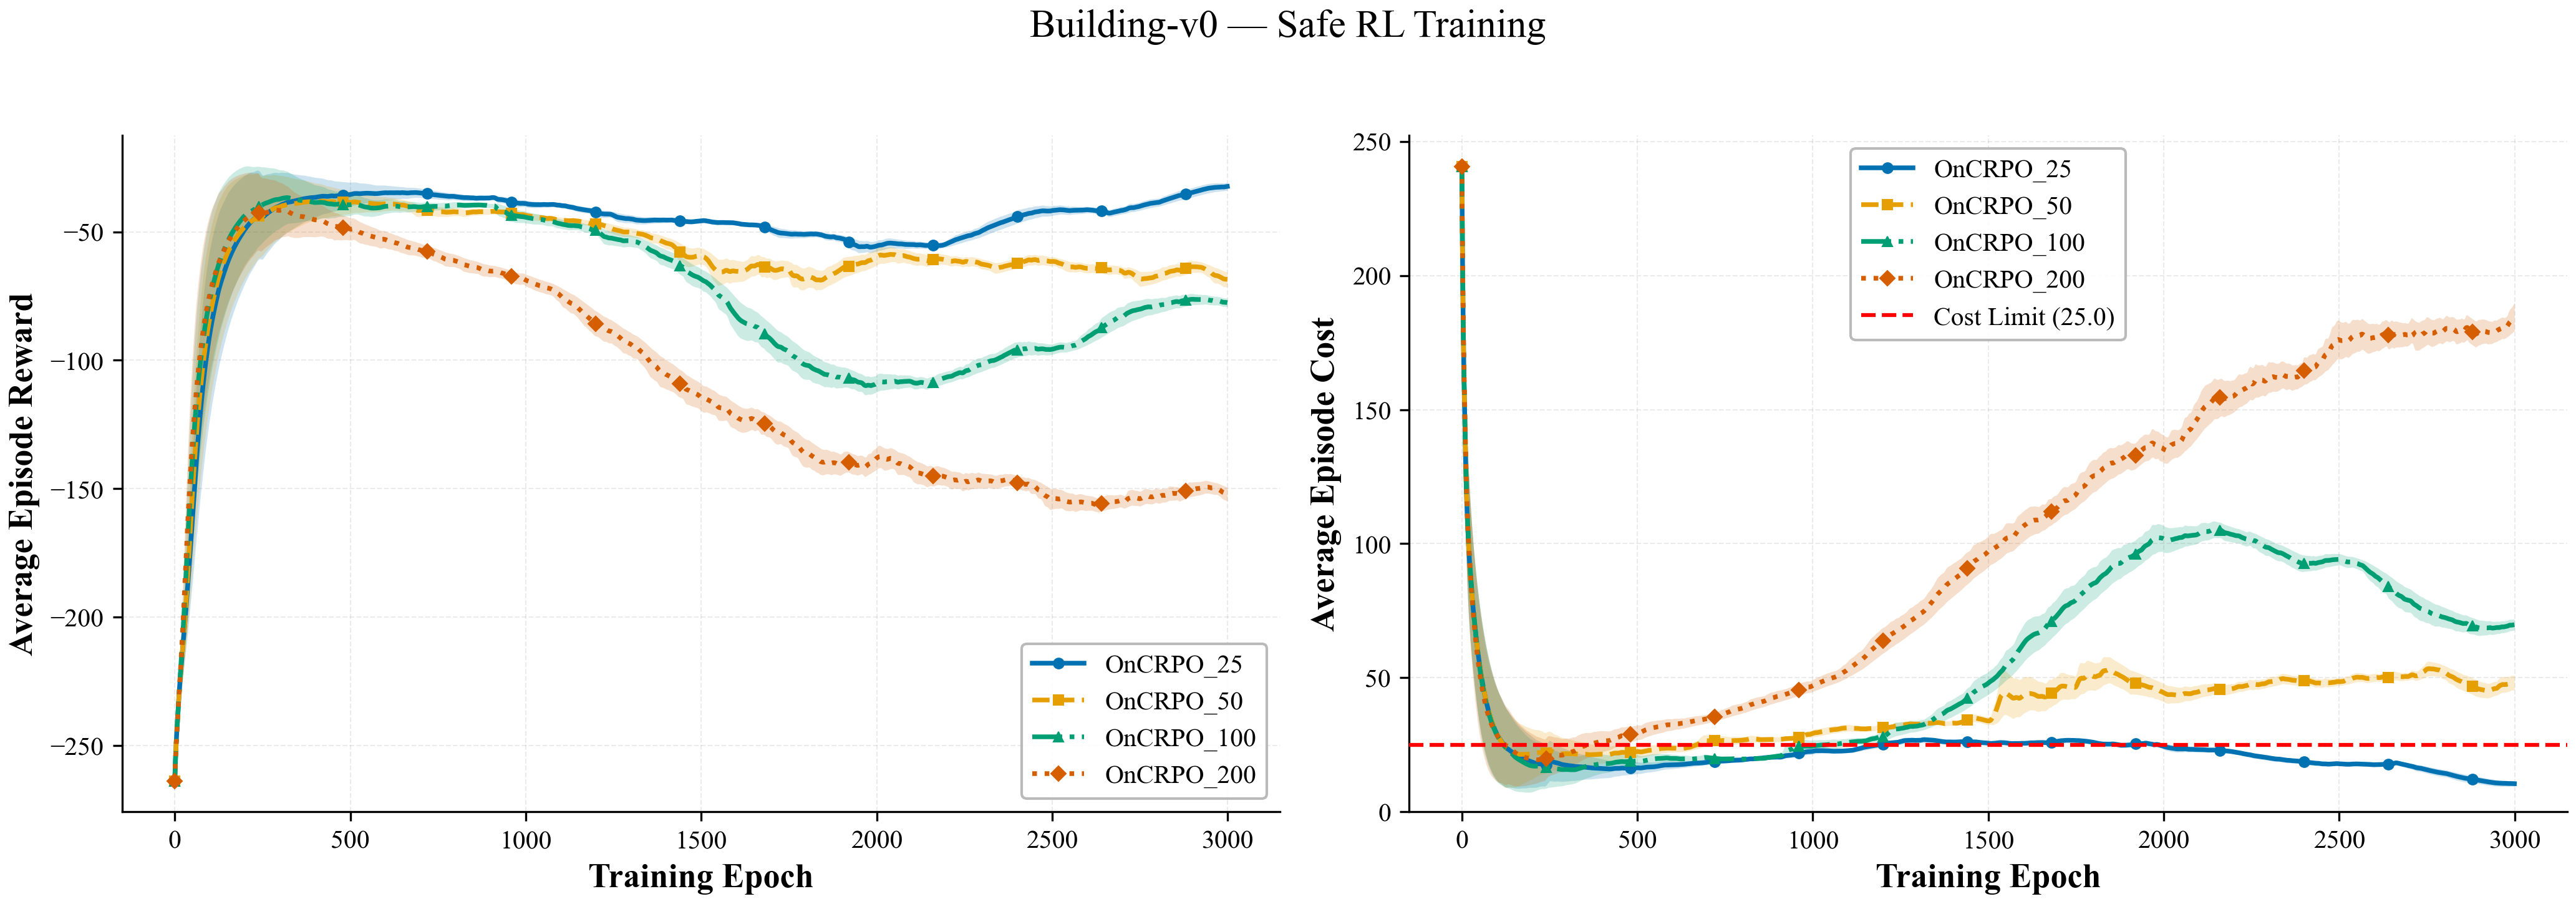
\includegraphics[width=0.9\textwidth]{figures/C_SRL/building/saferl_building_OnCRPO_3000ep_200ema.png}
\caption{Building OnCRPO: Similar divergence pattern to CPO at loose limits.}
\label{fig:srl_bu_oncrpo}
\end{figure}

% --- Building FOCOPS ---
\subsubsection{Building --- FOCOPS}

FOCOPS exhibits late-training cost increases at loose limits (\Cref{fig:srl_bu_focops}), indicating Lagrangian multiplier oscillation when the constraint is trivially satisfied.

\begin{figure}[htbp]
\centering
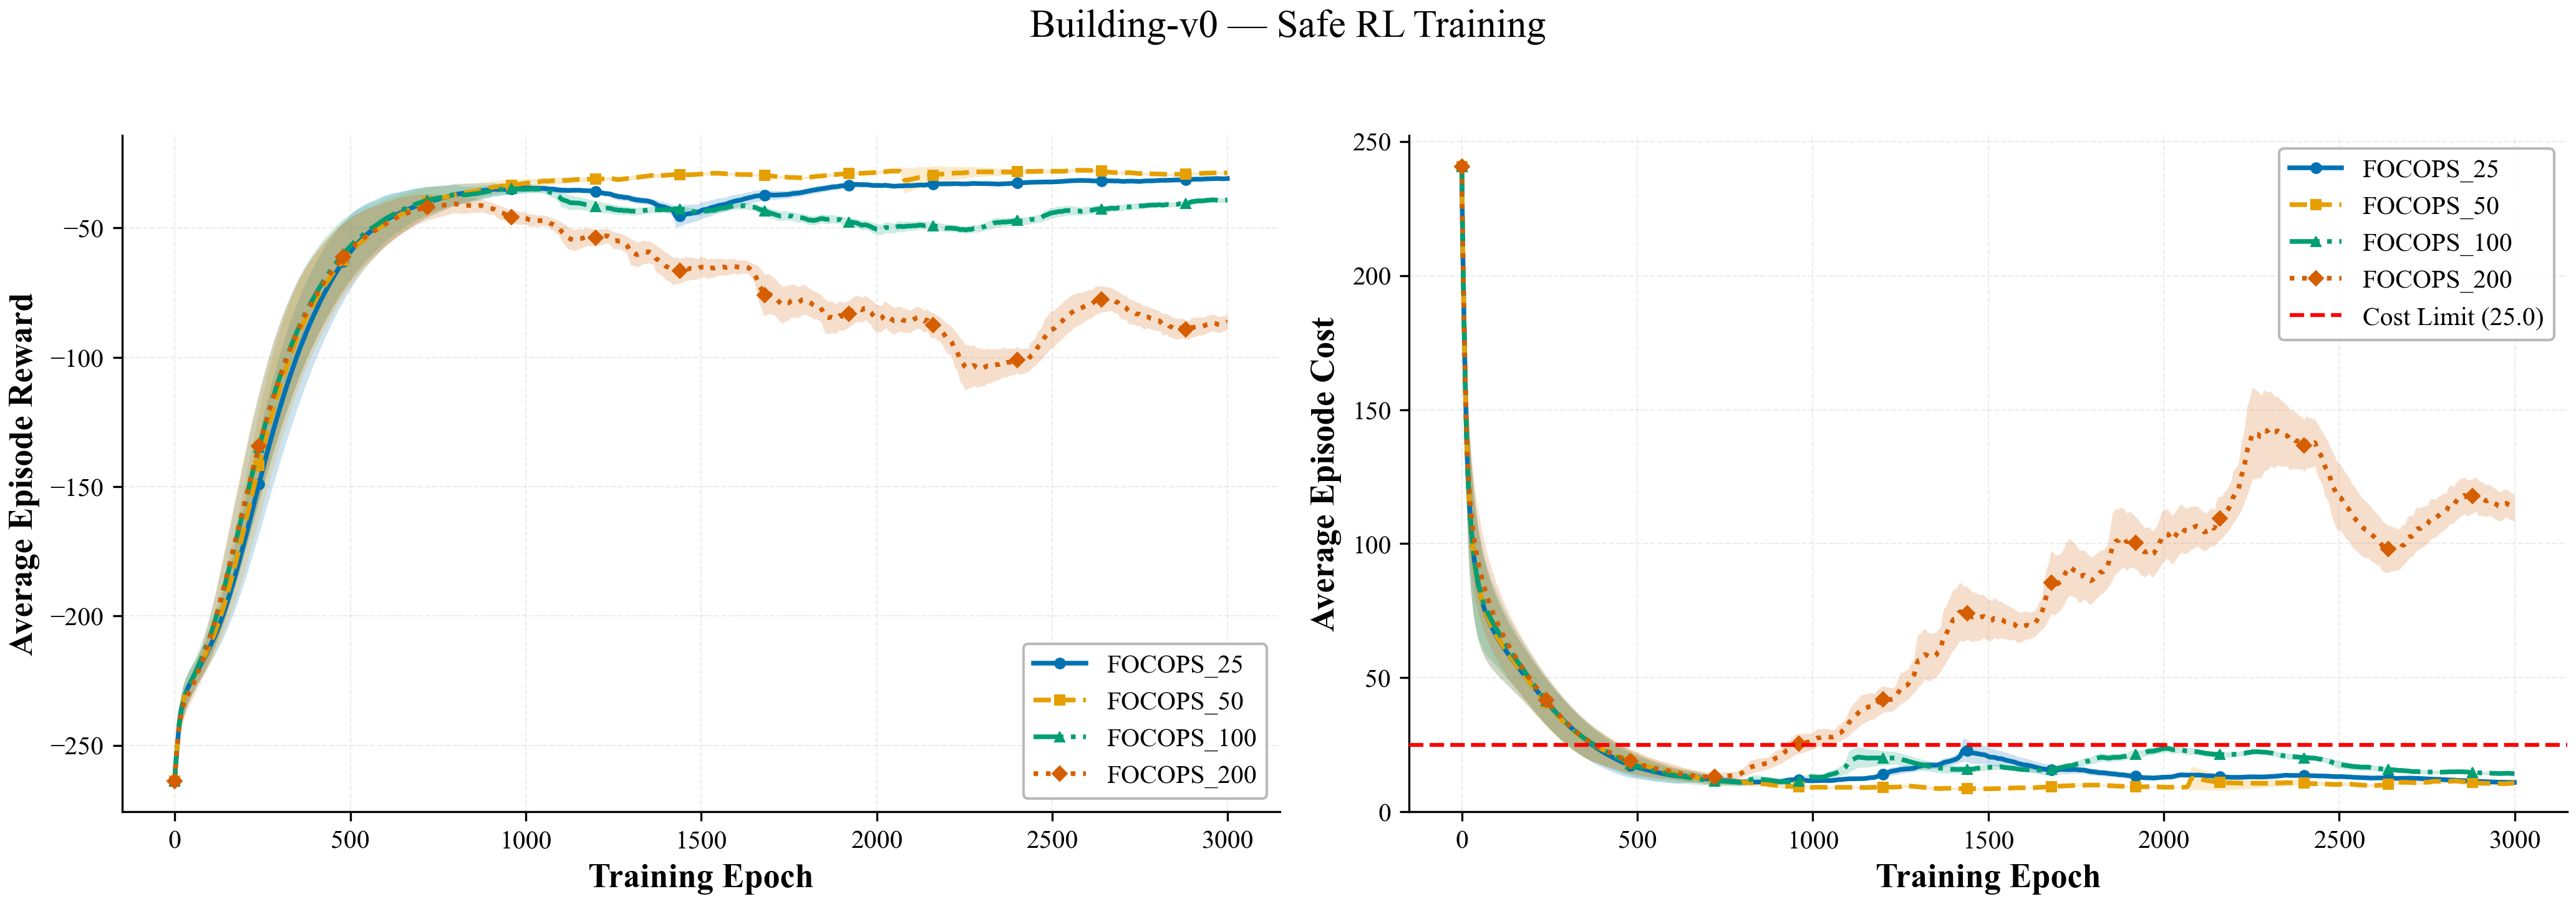
\includegraphics[width=0.9\textwidth]{figures/C_SRL/building/saferl_building_FOCOPS_3000ep_200ema.png}
\caption{Building FOCOPS: Late-training cost increase at loose limits indicates Lagrangian oscillation.}
\label{fig:srl_bu_focops}
\end{figure}

% ------------------------------------------------------------
\subsection{Off-Policy Safe RL: SACLag Failure}
\label{sec:saclag}

SACLag (SAC with Lagrangian relaxation) failed consistently across all three environments. The root cause is a fundamental incompatibility between replay buffer data staleness and Lagrange multiplier updates: the cost critic is trained on stale transitions, causing $\lambda$ to oscillate or diverge.

% ------------------------------------------------------------
\subsection{Safe RL Findings}

\begin{finding}[Reward--Cost Orthogonality Is Necessary (RQ4)]
\label{find:orthogonality}
CMDP formulations require the cost signal to measure an objective not adequately incentivized by the reward. When reward and cost are aligned (Building: $\beta = 0.5$ comfort term), constraints are trivially satisfied. When orthogonal (Cogen: ramp stress; EV: excess charge), CMDP enables precise safety--performance tradeoff control.
\end{finding}

\begin{finding}[PPOLag Is the Most Robust CMDP Algorithm (RQ4)]
\label{find:ppolag_best}
Across all environments, PPOLag provides the best cost limit differentiation, precise constraint tracking, and graceful degradation under inactive constraints ($\lambda \to 0 \Rightarrow$ standard PPO). Trust-region methods (CPO, OnCRPO) converge faster but are vulnerable to numerical instability under loose constraints.
\end{finding}

\begin{finding}[Off-Policy CMDP Methods Fail (RQ4)]
\label{find:saclag}
SACLag's replay buffer staleness prevents accurate Lagrange multiplier tracking. This negative finding suggests that on-policy methods are currently the only reliable approach for CMDP-based Safe RL.
\end{finding}

\begin{table}[htbp]
\centering
\caption{Summary of Safe RL effectiveness across environments.}
\label{tab:saferl_summary}
\begin{tabular}{@{}lcccc@{}}
\toprule
\textbf{Environment} & \textbf{Cost Signal} & \textbf{Orthogonal?} & \textbf{Differentiates?} & \textbf{Best Algo} \\
\midrule
Cogeneration & Turbine ramping & Yes & Yes & PPOLag \\
EV Charging & Excess charge & Yes & Yes (tight) & PPOLag \\
Building & Temp violation & No & No & N/A \\
\bottomrule
\end{tabular}
\end{table}

% ============================================================
\section{Multi-Agent Reinforcement Learning}
\label{sec:results_marl}

Multi-agent RL experiments are currently in progress using Ray RLlib with PettingZoo parallel environments. Preliminary results will be presented upon completion of the MARL training runs across all three environments (EVCharging: 54 agents, Building: AC-enabled zones, Cogen: 4 turbine agents).

% ============================================================
\section{Cross-Axis Discussion}
\label{sec:results_discussion}

The results across noise robustness and Safe RL reveal several cross-cutting insights.

\subsection{Environment Characteristics Matter More Than Algorithm Choice}

The most consistent finding across both experimental axes is that environment structure---not algorithm hyperparameters---determines the effectiveness of robustness and safety interventions:

\begin{itemize}
    \item \textbf{EV Charging} is inherently robust to noise (aggregate daily patterns are noise-resistant) and amenable to Safe RL (excess charge is orthogonal to profit).
    \item \textbf{Building} is inherently fragile to noise (thermal dynamics amplify errors) and resistant to Safe RL (reward already captures both objectives).
    \item \textbf{Cogeneration} shows algorithm-dependent noise sensitivity (PPO robust, SAC fragile) and strong Safe RL behavior (ramp stress is under-penalized in reward).
\end{itemize}

\subsection{PPO's Dual Advantage}

PPO emerges as the most robust algorithm across both axes: it tolerates noise better than SAC/TD3 (\Cref{sec:noise_ev,sec:noise_bu,sec:noise_co}) and provides the best CMDP constraint satisfaction as PPOLag (\Cref{sec:results_saferl}). This dual advantage stems from PPO's on-policy nature: conservative policy updates prevent both noise amplification and stale-data problems that plague off-policy methods.

\subsection{Implications for Sustainable Energy Systems}

The practical implications for real-world deployment are:

\begin{enumerate}
    \item \textbf{Sensor investment}: Observation noise is far more damaging than action noise, prioritizing sensor accuracy over actuator precision.
    \item \textbf{Safety constraint design}: CMDP constraints must measure genuinely under-optimized objectives; redundant constraints (already captured by reward) provide no benefit.
    \item \textbf{Algorithm selection}: PPO/PPOLag provides the best robustness--safety combination, despite SAC's superior clean-condition performance in some environments.
\end{enumerate}
